%----------------------------------------------------------------------------------------
%	PACKAGES AND OTHER DOCUMENT CONFIGURATIONS
%----------------------------------------------------------------------------------------


\documentclass[12pt,openright,oneside,final]{report}
\usepackage{generators/imports}
\makeglossaries

\renewcommand*{\acronymname}{List of Acronyms and Abbreviations}
\renewcommand{\glsnamefont}[1]{\textbf{#1}}

%Create acronyms here.
\newacronym{saas}{SaaS}{Software as a Service}
\newacronym{vcs}{VCS}{Version Control System}

%You can also do explanations.
\newglossaryentry{git}{name={Git},
    description={Git is a \gls{vcs} for tracking changes in computer files and coordinating work on those files among multiple people}}
\begin{document}
\begin{titlepage}

\newcommand{\HRule}{\rule{\linewidth}{0.5mm}} % Defines a new command for the horizontal lines, change thickness here

\center % Center everything on the page
 
%----------------------------------------------------------------------------------------
%	HEADING SECTIONS
%----------------------------------------------------------------------------------------

\textsc{\LARGE University of Bergen \\ Department of informatics}\\[1.5cm] % Name of your university/college

%----------------------------------------------------------------------------------------
%	TITLE SECTION
%----------------------------------------------------------------------------------------

\HRule \\[0.5cm]
\begin{Huge}
	\bfseries{Analysis of Word Embeddings: A Clustering and Topological Approach}\\[0.7cm] % Title of your document
\end{Huge}
\HRule \\[0.5cm]

%----------------------------------------------------------------------------------------
%	AUTHOR SECTION
%----------------------------------------------------------------------------------------

\large \emph{Author:} Jonas Folkvord Triki\\
\large \emph{Supervisor:} Nello Blaser\\[2cm]

%----------------------------------------------------------------------------------------
%   LOGO SECTION
% 	This will require the graphicx package
%	Change the line to comment if you only want the UiB Logo
%	Logo for other faculties here: http://kapd.h.uib.no/profilmanual/99LastNed/99a_lastned.html
%----------------------------------------------------------------------------------------

\centerline{
\includegraphics[scale=1.9]{figures/canvasWithFaculty}}
%\centerline{
\includegraphics[scale=0.15]{figures/canvas}}  %change for your faculty

%----------------------------------------------------------------------------------------
%	DATE SECTION
%----------------------------------------------------------------------------------------

{\large June, 2021}\\[3cm] % Date, change the \today to a set date if you want to be precise

%----------------------------------------------------------------------------------------
%	LOGO SECTION
%----------------------------------------------------------------------------------------

\vfill % Fill the rest of the page with whitespace

\end{titlepage}
 % This is the titlepage
\pagenumbering{roman}

\begin{abstract}
\noindent
Over the last few years, advances in natural language processing (NLP) have enabled us to learn more from textual data. To this end, word embedding models learn vectorized representations of words by training on big sets of texts (e.g. the entire Wikipedia corpus). Word2vec is a word embedding model which learns a single vector representation for each word it is trained on. However, by creating single vector representations for words, it becomes hard to separate between word meanings. Words with multiple meanings are called \textit{polysemous}, and determining the word meanings of a given word is a difficult problem in NLP. Traditionally, word embeddings from word2vec are analyzed using analogy and cluster analysis. In analogy analysis of word embeddings, it is common to show relationships between words, i.e that the relationship between \textit{king} and \textit{man} is same as that between \textit{queen} and \textit{woman}. Moreover, in cluster analysis of word embeddings, it is commonly shown that similar words cluster together, such as colours, names and countries. Additionally, recent developments in the field of topological data analysis (TDA) introduces a topological measure of polysemy, which attempts to identify polysemous words from their word embeddings. The goal of this thesis is to show how word embeddings traditionally are analyzed using analogies and clustering algorithms, and additionally, to use methods such as topological polysemy to identify polysemous words, using various word embeddings. Our results show that we are effectively able to cluster word embeddings into groups of varying sizes. Results also revealed that the measure of topological polysemy was inconsistent across word embeddings, and our proposed supervised models attempt to overcome and improve on this work.
\end{abstract}

\renewcommand{\abstractname}{Acknowledgements}
\begin{abstract}
I would first and foremost like to thank my supervisor, Nello Blaser, for his outstanding guidance during the work of this thesis.

I would also like to thank my fellow graduate students, particularly Naphat, for the long lunch breaks and the helpful academic discussions.

Finally, I would like to thank my friends and family for all their love and support.

\textbf{TODO}: Add to the acknowledgements.

\vspace{1cm}
\hspace*{\fill}\texttt{Jonas Folkvord Triki}\\ 
\hspace*{\fill} 01 June, 2021
\end{abstract}
\newpage
{\tableofcontents \let\cleardoublepage\clearpage \listoffigures \let\cleardoublepage\clearpage \listoftables \let\cleardoublepage\clearpage \lstlistoflistings}
\setcounter{secnumdepth}{4}
\setcounter{tocdepth}{4}
\pagenumbering{arabic}
\setcounter{page}{1}
\setlength{\parskip}{0.5cm plus4mm minus3mm}  

\chapter{Introduction}
\label{chap:introduction}
Natural language processing (NLP) is a field of study which focuses on the interactions between computers and the natural human language. In modern NLP applications, it is common to see the usage of vector embedding algorithms, such as the word2vec techniques introduced in \cite{mikolov2013a}. Word2vec learns vectorized representations of words (called word embeddings) by training on big text sets (e.g. whole Wikipedia). Word embeddings are created such that the semantics of a word is reflected by its word embedding. For example, the word \textit{solution} is similar to the word \textit{chemistry}, but is also related to words such as \textit{answer} or \textit{equation}. By inspecting the word embeddings of such words, we find that they are highly similar. Furthermore, we also see that the word \textit{solution} can have multiple meanings, depending on the context it is used in. We call such words \textit{polysemous}, and the task of determining polysemous words in NLP is a difficult problem. To measure and determine polysemous words from word embeddings, the measure of topological polysemy was introduced in \cite{jakubowski2020topology}. The topological polysemy method seeks to identify singular word embeddings, which the authors claim reflect polysemy.

Classically, word embeddings are analyzed using analogy and cluster analysis. In this thesis, we will first perform a similar analogy and cluster analysis, by using general methods from machine learning, and among these, clustering algorithms and dimensionality reduction methods. The goal is to find a richer description of word embeddings. In particular, we will first explain how we trained and evaluated our word2vec model, before proceeding onto clustering of word embeddings using clustering algorithms. We will validate the results from the cluster analysis using internal cluster validation methods and visualize our results using dimensionality reduction methods. After performing the cluster analysis on word embeddings, we will in this thesis investigate the method of topological polysemy by applying it to various word embedding models. Our goal is to recreate the results shown in \cite{jakubowski2020topology} for a general word embedding model, which further strengthens their proposed method and results. We will also look at another algorithm called Geometric Anomaly detection (GAD). GAD seeks to identify singular points in the data, similar to what the topological polysemy method does. Following, we will compare the results using topological polysemy and GAD to show their relation. Next, we look at the application of intrinsic dimension estimation (ID) methods on word embeddings and show the relationship between the estimated local ID of a word to the number of word meanings. We would like to, in particular, see if the estimated local ID of word embeddings can help us to predict the number of word meanings. Finally, we propose two supervised methods for predicting polysemous words, using results from topological polysemy, GAD and ID estimation methods.

This thesis is structured as follows. In \cref{chap:background} we give the technical and theoretical background required for this thesis. Following, in \cref{chap:analysis-of-word-embeddings} we perform our analysis of word embeddings, explaining training and evaluation steps for our word2vec model, perform clustering of word embeddings, and finally, analyze methods for polysemous words prediction. In \cref{chap:summary-and-conclusion}, we summarize and conclude the thesis. Lastly, in \cref{chap:future-work} we look at ideas for future work related to the thesis.
\chapter{Background}
\label{chap:background}
In this chapter, we will introduce and explain the technical and theoretical background of this thesis. In particular, we will introduce general methods from machine learning, the notion of word embeddings, and topological data analysis (TDA) and methods from its field. We will describe concepts to the point where they are understandable for the sake of the thesis, but leave out technical details of concepts that are not in focus (e.g. intrinsic dimension estimation in \cref{sec:intrinsic-dimension-estimation}). On the other hand, we have some particular concepts which we have worked with more extensively throughout the thesis, such as clustering (\cref{sec:clustering-algorithms,sec:cluster-validation}), word embeddings (\cref{sec:word-embeddings}), and TDA (\cref{sec:topological-data-analysis}). Thus, we will give a thorough explanation of these concepts. Finally, we assume that the reader is familiar with general concepts from calculus, linear algebra, and statistics. In the following sections, we will introduce and explain the technical and theoretical background of this thesis.

% Add sections
\section{General machine learning methods}
In this section, we will introduce and explain general machine learning methods. In particular, we will first define machine learning in \cref{sec:what-is-machine-learning}, then move onto clustering algorithms and validation of clusters in \cref{sec:clustering-algorithms,sec:cluster-validation}. Following, we will describe two methods for performing dimensionality reduction in \cref{sec:dimensionality-reduction-methods}, explain the concept of artificial neural networks in \cref{sec:artificial-neural-networks} and intrinsic dimension estimation in \cref{sec:intrinsic-dimension-estimation}. Finally, we round the section by explaining methods from regression analysis in \cref{sec:regression-analysis}, how to perform model selection in \cref{sec:model-selection} and introduce performance metrics in \cref{sec:performance-metrics}.

\subsection{What is machine learning?}
\label{sec:what-is-machine-learning}
In traditional computer programs, we typically create the rules and instructions of the program to get the output we desire. In \textit{machine learning} (ML), however, we turn the problem on its head, and the goal is to learn the rules of the program using its input data \cite{Mitchell1997}. More formally, we quote the famous definition from \cite[p. 2]{Mitchell1997} to define ML: \say{A computer program is said to learn from experience $E$ with respect to some class of tasks $T$ and performance measure $P$ if its performance at tasks in $T$, as measured by $P$, improves with experience $E$}. To give an example, let $E$ be data of whether or not it has rained the last seven days in Bergen, and let $T$ be the task of determining if it rains the next day. To measure the performance $P$, we use the percentage of correct guesses for whether or not it rains the next day. The ML program can then use the data from experience $E$ to improve on the task $T$ by maximizing the performance $P$. Furthermore, we further motivate the use of machine learning by illustrating with an example in \cref{fig:ml-versus-tradional-programming}, where we see the differences between traditional programming and machine learning programs.
\begin{figure}[H]
    \centering
    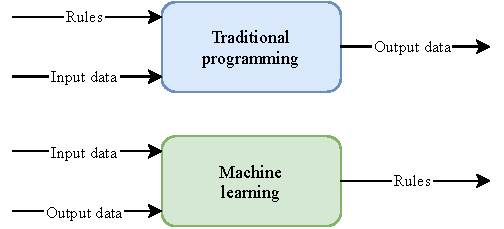
\includegraphics[width=0.7\textwidth]{thesis/figures/ml-versus-tradional-programming_cropped.pdf}
    \caption{Traditional programming compared to machine learning.}
    \label{fig:ml-versus-tradional-programming}
\end{figure}

In this thesis, we will in particular look at two approaches for ML, namely \textit{supervised} and \textit{unsupervised learning}. In a supervised learning setting, we give the ML program its input and output data. The goal is to learn the parameters of the ML program to map the input data to the output data. In an unsupervised learning setting, however, we do not give the ML program any output data, leaving the ML program to find structure in its input data. The goal of unsupervised ML programs is to discover and learn hidden patterns from the input data, by applying (possibly) several methods. In this thesis, we will learn from data by mainly using unsupervised ML methods (e.g. cluster analysis and dimensionality reduction in \cref{sec:analysis-of-word-embeddings-word-clustering}), but also some supervised ML methods (e.g. supervised polysemy prediction in \cref{sec:analysis-of-embeddings-supervised-polysemy-prediction}) as well. In the following subsections, we will introduce and explain general methods and concepts from machine learning.

\subsection{Clustering algorithms}
\label{sec:clustering-algorithms}
In a supervised machine learning setting, we typically use data $X$ and its associated labels $y$. The supervised task is to train a model to predict the labels $y$ using the data $X$. A classical example of a supervised machine learning task is to distinguish between dogs and cats, where $X$ is an image of a dog or a cat and the labels $y$ indicate whether or not the data $X$ represents a dog ($y=0$) or a cat ($y=1$). In an unsupervised setting, however, the labels $y$ are less likely to be present. To predict the labels $y$, we apply \textit{clustering algorithms}.

Clustering is one of the most important methods in unsupervised machine learning. Clustering algorithms divide some data $X$ into clusters (groups) such that the data in each cluster are similar in some sense. An example of this is clustering by using \textit{Euclidean distance}, which measures the distance of a line segment between two points $u$ and $v$. More formally, we define the Euclidean distance between two points $u$ and $v$ as
\begin{align}
    d(u, v) = ||u-v||_2 = \sqrt{\enclp{u_1 - v_1}^2 + \enclp{u_2 - v_2}^2 + \ldots + \enclp{u_n - v_n}^2},
    \label{eqn:euclidean-distance}
\end{align}
where $u$ and $v$ are two $n$-dimensional vectors. If we cluster by Euclidean distance, we want the distance between any two data points belonging to the same cluster to be small. We refer this distance as the \textit{intracluster distance} or \textit{compactness}. Unfortunately, it is usually not enough to only minimize the intracluster distance; we also have to ensure that the distance between the clusters is as large as possible. To measure the distance between two clusters we measure the distance between two data points belonging to different clusters. We refer this distance as the \textit{intercluster distance} or \textit{separation}. If a clustering algorithm can create clusters such that we have small intracluster distance and large intercluster distance, it indicates that the clustering algorithm is good for the data at hand. We note, however, that data can be very complex and it can be very hard to find good clusters. In the following sub-subsections, we look at some common clustering algorithms, explain how they work, and discuss their strengths/weaknesses. In each of the clustering algorithms, we assume that we have some data $X = \enclc{x_1, x_2, \ldots, x_n} \in \R^{n \times d}$. Furthermore, we will use the clustering algorithms below in the analysis of word embeddings (\cref{sec:word-embeddings}) in \cref{chap:analysis-of-word-embeddings}.

\subsubsection{k-means clustering}
\label{sec:k-means-clustering}
The \textit{k-means clustering} method is an unsupervised machine learning algorithm for identifying clusters in data \cite[Section 9.1]{bishop2006}. The algorithm uses an iterative approach to search for $k$ clusters, where $k$ is a \textit{hyperparameter} (i.e. in control by user). There exist several variants of this algorithm and we discuss two of them in later sub-subsections (see \cref{sec:mini-batch-k-means-clustering} and \cref{sec:k-medoids-clustering}). Following, we explain the standard (and naïve) variant of the algorithm (i.e. \textit{Lloyd's algorithm}), and we base this sub-subsection on \cite[Section 9.1]{bishop2006}.

The standard k-means clustering algorithm works as follows. The first step is to determine the initial cluster means, or \textit{centroids}. Since we want the algorithm to output $k$ clusters, we have to decide $k$ initial centroids. The simplest way to do this is to select $k$ random data points to be the initial $k$ centroids. The next step is to calculate the Euclidean distance between each data point to the cluster centroids. We do so because we want to determine which cluster each data point belongs to. Furthermore, we assign each data point to its closest cluster centroid and compute the mean of each cluster. The third and final step is to move the cluster centroid to the new mean of each cluster. We repeat the second and third steps until convergence is met (e.g. change of loss is less than a set threshold). Finally, we illustrate the use of k-means clustering in \cref{fig:k-means-clustering-2d-example}, where we see its cluster boundaries, representing the clusters. The white crosses represent the cluster centroids.
\begin{figure}[H]
    \centering
    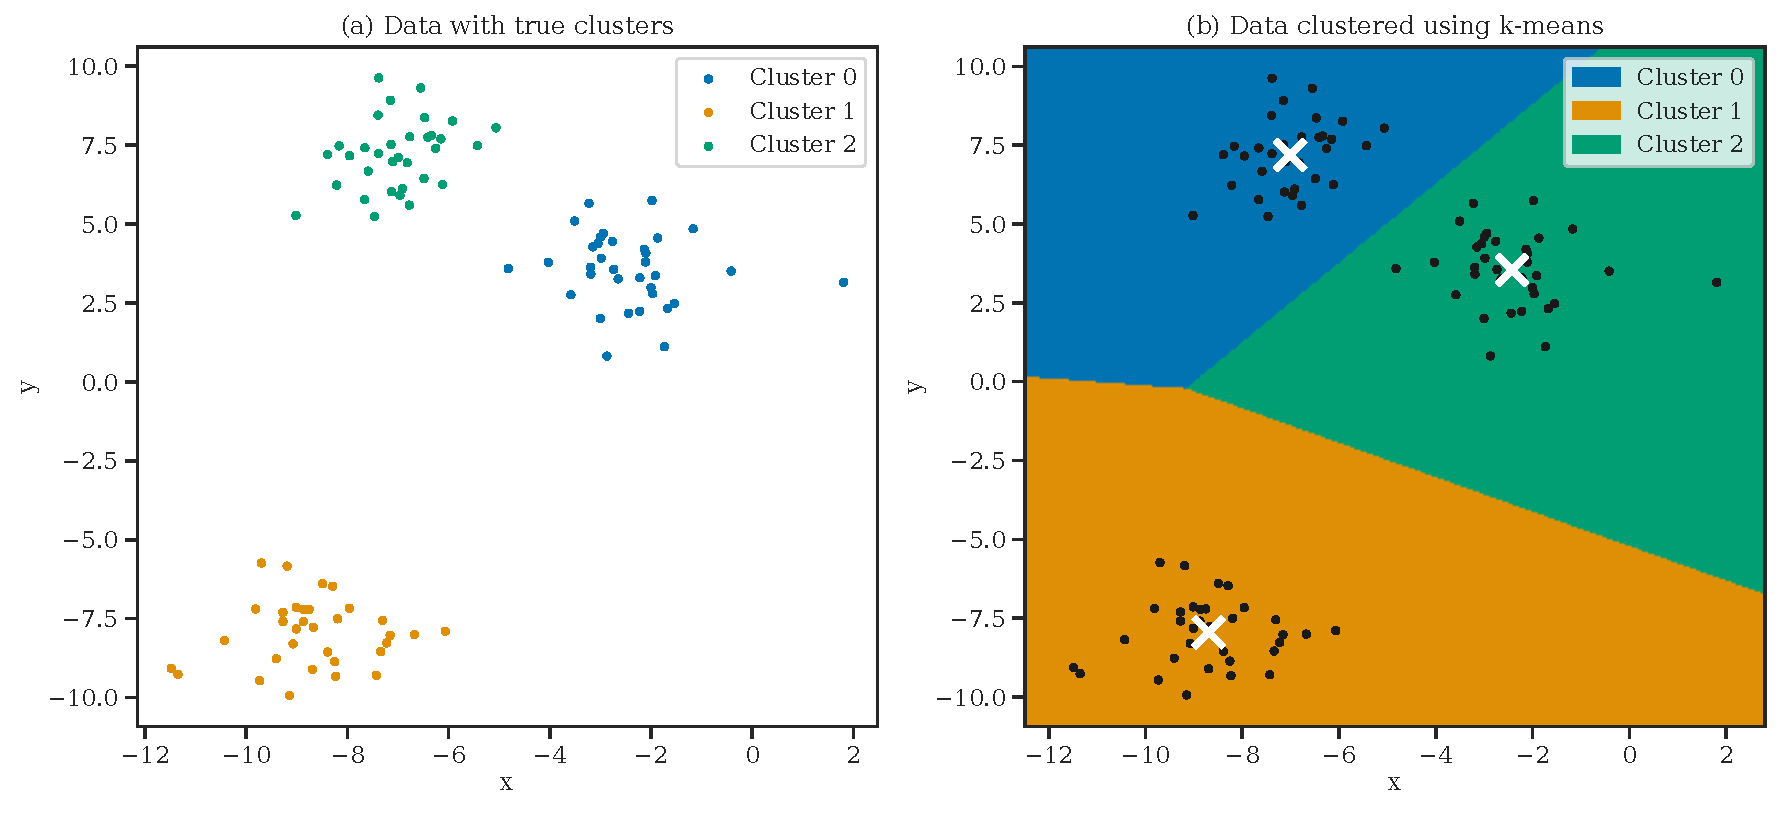
\includegraphics[width=\textwidth]{thesis/figures/k-means-clustering-2d-example.pdf}
    \caption{Example of clustering using k-means clustering on a 2-dimensional data set with 3 clusters. We show the cluster boundaries in (b), emphasized by the colours.}
    \label{fig:k-means-clustering-2d-example}
\end{figure}

Mathematically, the goal of k-means clustering is to minimize the squared distance between the points in each cluster to its respective centroid, which we refer to as the within-cluster sum of squares (WCSS). The objective is to find
\begin{align}
    \argmin_{C} \sumlim{i=1}{k} \sumlim{x \in C_i}{} \norm{x - \mu_i}^2,
\end{align}
where $C = \enclc{C_1, C_2, \ldots, C_k}$ are the clusters of the data $X$, $k$ is a hyperparameter for the number of clusters and $\mu_i$ is the cluster centroid of cluster $C_i$.

The main advantage of k-means clustering is its simplicity, both in implementation and when interpreting the results. The algorithm also scales well to larger data sets, and there is only one hyperparameter to tune (number of clusters $k$). As for the disadvantages, the algorithm is rather sensitive to the initialization of centroids in the first step. If we were to select very bad initial centroids, the convergence time of the algorithm increases greatly, and we end up with bad clusters. We also have to choose the number of clusters manually, which is a downside if we have no additional knowledge of the data beforehand. In addition to this, the algorithm suffers from the \textit{curse of dimensionality}, which is a set of problems that can occur when analyzing high-dimensional data (i.e. greater than two to three dimensions). In the context of k-means clustering, as the dimensionality increases, it becomes more and more difficult to distinguish between data points (all points converge to the same distance). We illustrate an effect of the curse of dimensionality in \cref{fig:curse-of-dimensionality}.
\begin{figure}[H]
    \centering
    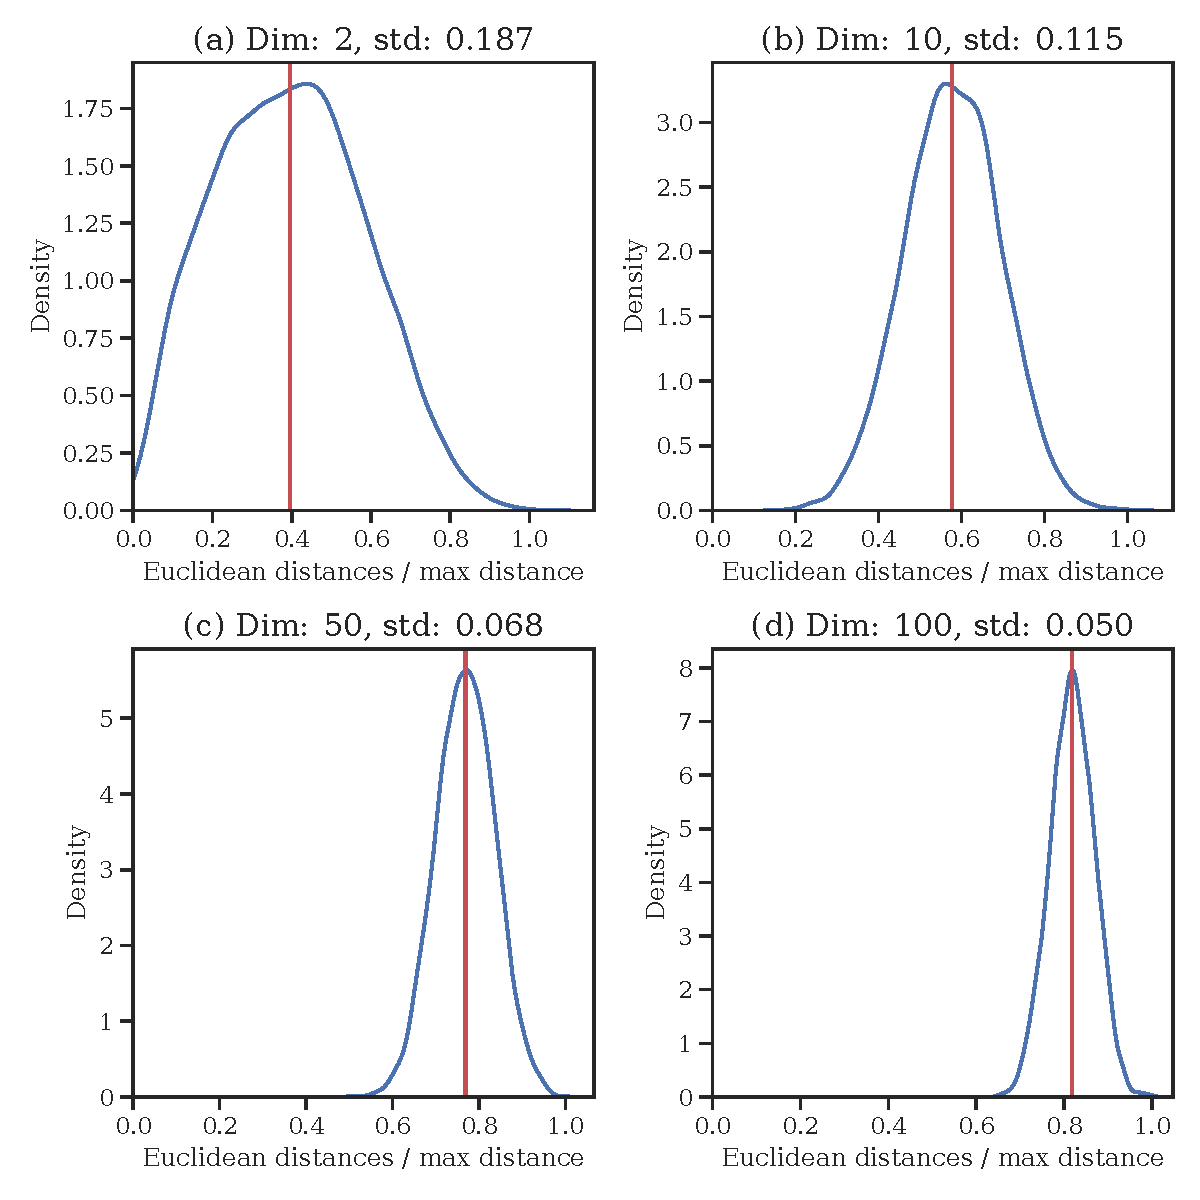
\includegraphics[width=0.9\textwidth]{thesis/figures/curse-of-dimensionality.pdf}
    \caption{Four illustration plots showing an effect of the curse of dimensionality. The distance between points in higher dimensional spaces becomes the same as the dimensionality increases, and thus, it is harder to differentiate between points using distance metrics. The blue line represents the density of the pairwise Euclidean distances (we divide by the max distance to normalize the x-axis). The red line is the mean distance.}
    \label{fig:curse-of-dimensionality}
\end{figure}

\subsubsection{Mini-batch k-means clustering}
\label{sec:mini-batch-k-means-clustering}
\textit{Mini-batch k-means clustering} is a variant of k-means clustering, where we use \textit{mini-batches} of data points to find a suitable clustering \cite{sculley2010}. To create the mini-batches, we randomly sample subsets of the training data for each training iteration (similar to the mini-batches in gradient descent from \cref{sec:ann-optimizers}). We refer to \cite{sculley2010} when explaining mini-batch k-means clustering.

The algorithm is very similar to the standard k-means clustering algorithm and comprises two major steps. In the first step, we initialize $k$ cluster centroids and sample $B=\enclc{b_1, b_2, \ldots, b_m} \subset X$ points at random from the data set $X$, where $m$ is the mini-batch size. In the second step, we update the cluster centroids by gradually moving the centroids. For each sample $b$ in the mini-batch, we update the centroids by taking the average of $b$ and the previous points assigned to the centroid. By doing so, we move the centroid with a decreasing rate over time. We repeat the first and second steps until convergence is met (e.g. change of loss is less than a set threshold).

The main advantage of mini-batch k-means clustering over standard k-means is that the convergence time is lower. By using mini-batches, we drastically reduce the computational requirement for converging to a local solution and, the results of mini-batch k-means clustering tend to only be slightly worse than the standard algorithm.

\subsubsection{k-medoids clustering}
\label{sec:k-medoids-clustering}
\textit{K-medoids clustering} is an alternative to the standard k-means clustering algorithm \cites{Kaufman1990}[p. 427 - 428]{bishop2006}. K-medoids clustering uses data points for its cluster centroids and works with any dissimilarity measure. A \textit{medoid} of a cluster is a data point where the average dissimilarity between the medoid and all other data points in the same cluster is minimal. We refer to \cites{Kaufman1990}[p. 427 - 428]{bishop2006}\, when explaining k-medoids clustering.

To solve the k-medoids problem efficiently, we use the \textit{Partitioning Around Medoids} (PAM) algorithm. Similar to the standard k-means clustering algorithm, PAM consists of two main stages, namely the \textit{build-} and \textit{swap} stages. In the build stage, we greedily select $k$ of the $n$ data points to be the initial cluster medoids, which we denote $M = \enclc{m_1, m_2, \ldots, m_k} \subset X$. To select $M$ initially, we want to minimize the dissimilarity between the cluster medoids and points in the same cluster. In other words, initially, we set the first medoid $m_1$ to be the data point such that the dissimilarity between then medoid and all other data points is minimal. Then, for all proceeding medoids ($m_2, \ldots, m_k$), we look for medoids such that the dissimilarity between the additional medoid, the data points in the same cluster as the new medoid, and all other medoids (and its cluster data points) is minimal. We repeat this process until we have $k$ medoids. Following, the swap stage consists of iteratively swapping out the $k$ medoids with other data points from the data set, if it minimizes the overall dissimilarity. The algorithm terminates if by swapping the medoids with other data points we do not get lower dissimilarity. Finally, we illustrate the use of k-medoids clustering in \cref{fig:k-medoids-clustering-2d-example}, where we see that each point is connected to its cluster by a line, signalizing the dissimilarity between the points and the cluster medoids. The black dots represent the cluster medoids.
\begin{figure}[H]
    \centering
    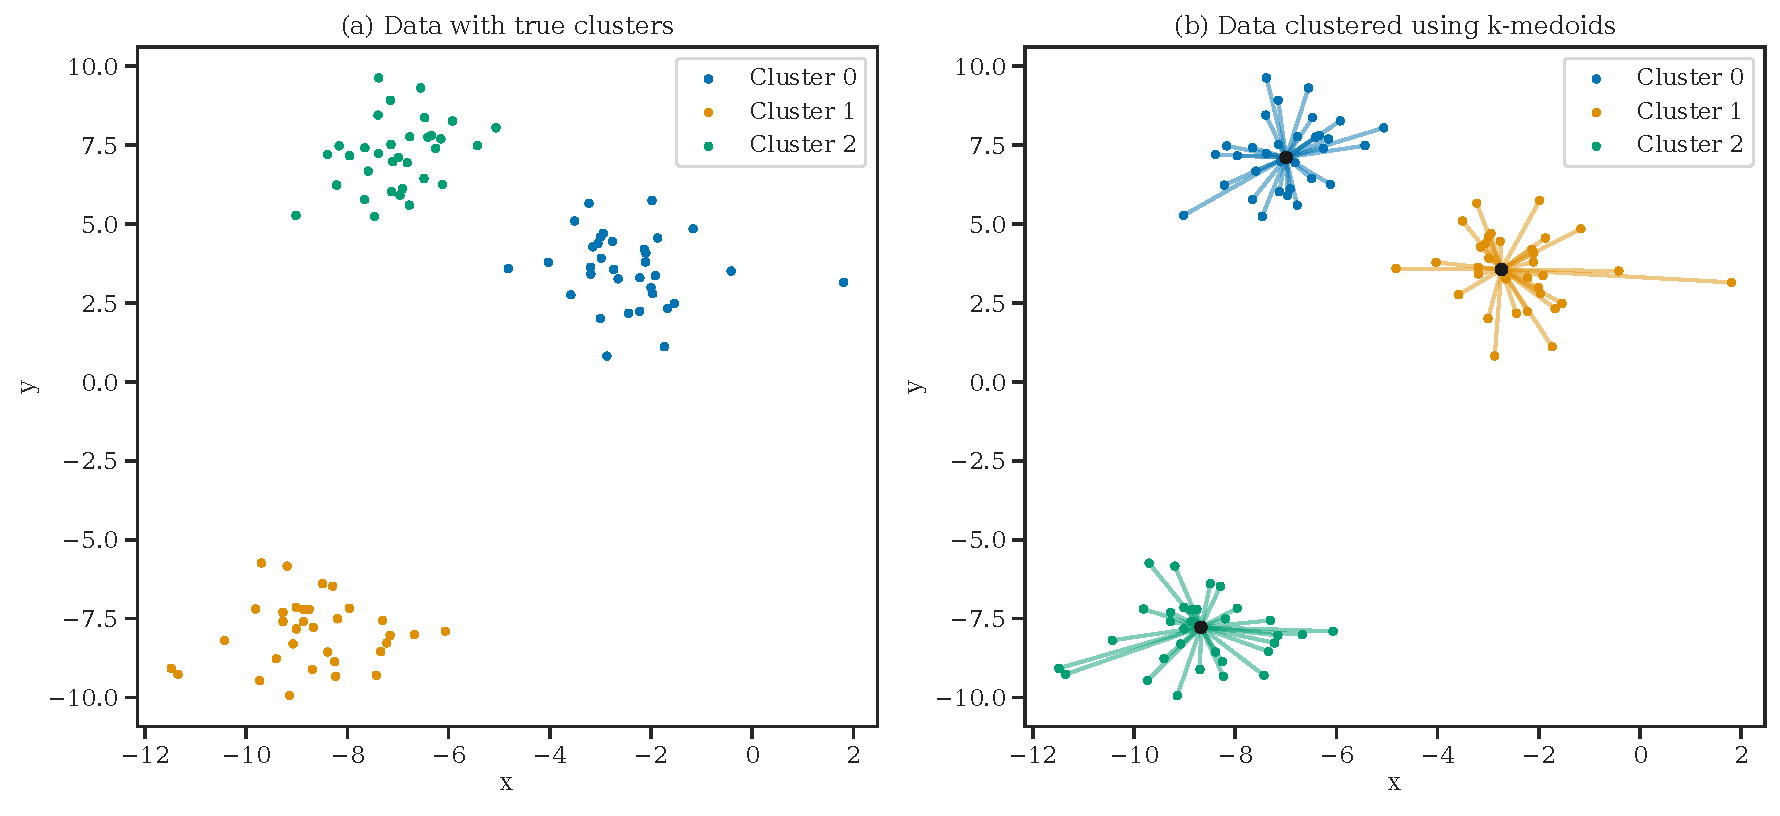
\includegraphics[width=\textwidth]{thesis/figures/k-medoids-clustering-2d-example.pdf}
    \caption{Example of clustering using k-medoids clustering on a 2-dimensional data set with 3 clusters. The lines signalize dissimilarity between points and the cluster medoids.}
    \label{fig:k-medoids-clustering-2d-example}
\end{figure}

The main advantage of k-medoids is that it is more interpretable and robust to outliers than the standard k-means clustering algorithm since it uses actual data points as centroids. In addition to this, we may use any dissimilarity measure, whereas, in the standard k-means clustering, Euclidean distance is the only option. Even though k-medoids clustering seems to be the superior choice over k-means clustering, it suffers from the fact it is more computationally heavy to compute and thus is not always feasible to run for large data sets.

\subsubsection{Gaussian mixture models}
\label{sec:gmm-clustering}
\textit{Gaussian mixture models} (GMMs) are probability distributions which consists of a mixture of multiple \textit{Gaussians} \cite[Section 9.2]{bishop2006}. A Gaussian (i.e. normal) is a probability distribution which was several nice properties, such as mean as its mode and symmetry. In the context of cluster algorithms, we use GMMs to cluster data points by using multivariate (i.e. of higher dimension) Gaussian distributions as cluster centroids. In particular, for each cluster centroid $c_i, 1 \leq i \leq k$, we define $\mu_i$ to be the cluster mean, $\Sigma_i$ to be the cluster covariances and $\pi_i$ to be the \textit{mixing coefficients}. The cluster means $\mu_i$ and covariances $\Sigma_i$ determines the localization and spread for each cluster, while the mixing coefficients $\pi_i$ determine how much we emphasize each cluster. To estimate the parameters $\theta = \enclc{\mu, \Sigma, \pi}$ of GMMs, we use the Expectation-Maximization (EM) algorithm, which is an iterative algorithm. When explaining GMMs and the EM algorithm, we refer to \cite[Section 9.2]{bishop2006}.

The EM algorithm starts by initializing its parameters $\mu$, $\Sigma$, and $\pi$. There exist several methods for initializing the parameters and it is common to first run k-means clustering on the data to obtain a suitable starting point. By running k-means clustering first, we compute the initial parameters by using statistics from the result of k-means. Furthermore, the EM algorithm consists of two main stages, namely \textit{expectation} and \textit{maximization}. In the expectation stage, we compute the responsibilities for each data point in $X$ using the current set of parameters. With responsibilities, we mean how much each Gaussian is responsible for explaining a single data point in $X$. Next, in the maximization step, we use the responsibilities from the expectation step to update the parameters such that the likelihood $\text{P}(X | \theta)$ is maximal. The likelihood $\text{P}(X | \theta)$ tells us how good the set of parameters $\theta$ fits our data $X$. The exact derivation and update rules for each parameter are left out and we refer the reader to \cite[Section 9.4]{bishop2006} for more details. Once a suitable threshold is met with respect to $\text{P}(X | \theta)$, the algorithm terminates and we converge to a set of parameters $\hat{\theta}$. Using the final parameters, $\hat{\theta}$, we predict which Gaussian (i.e. cluster) to associate for every data point $x \in X$, by selecting the Gaussian with the highest density. Finally, we illustrate the effect of GMM clustering in \cref{fig:k-gmm-clustering-2d-example}, where we see that the different clusters have different shapes (i.e. means and covariances).
\begin{figure}[H]
    \centering
    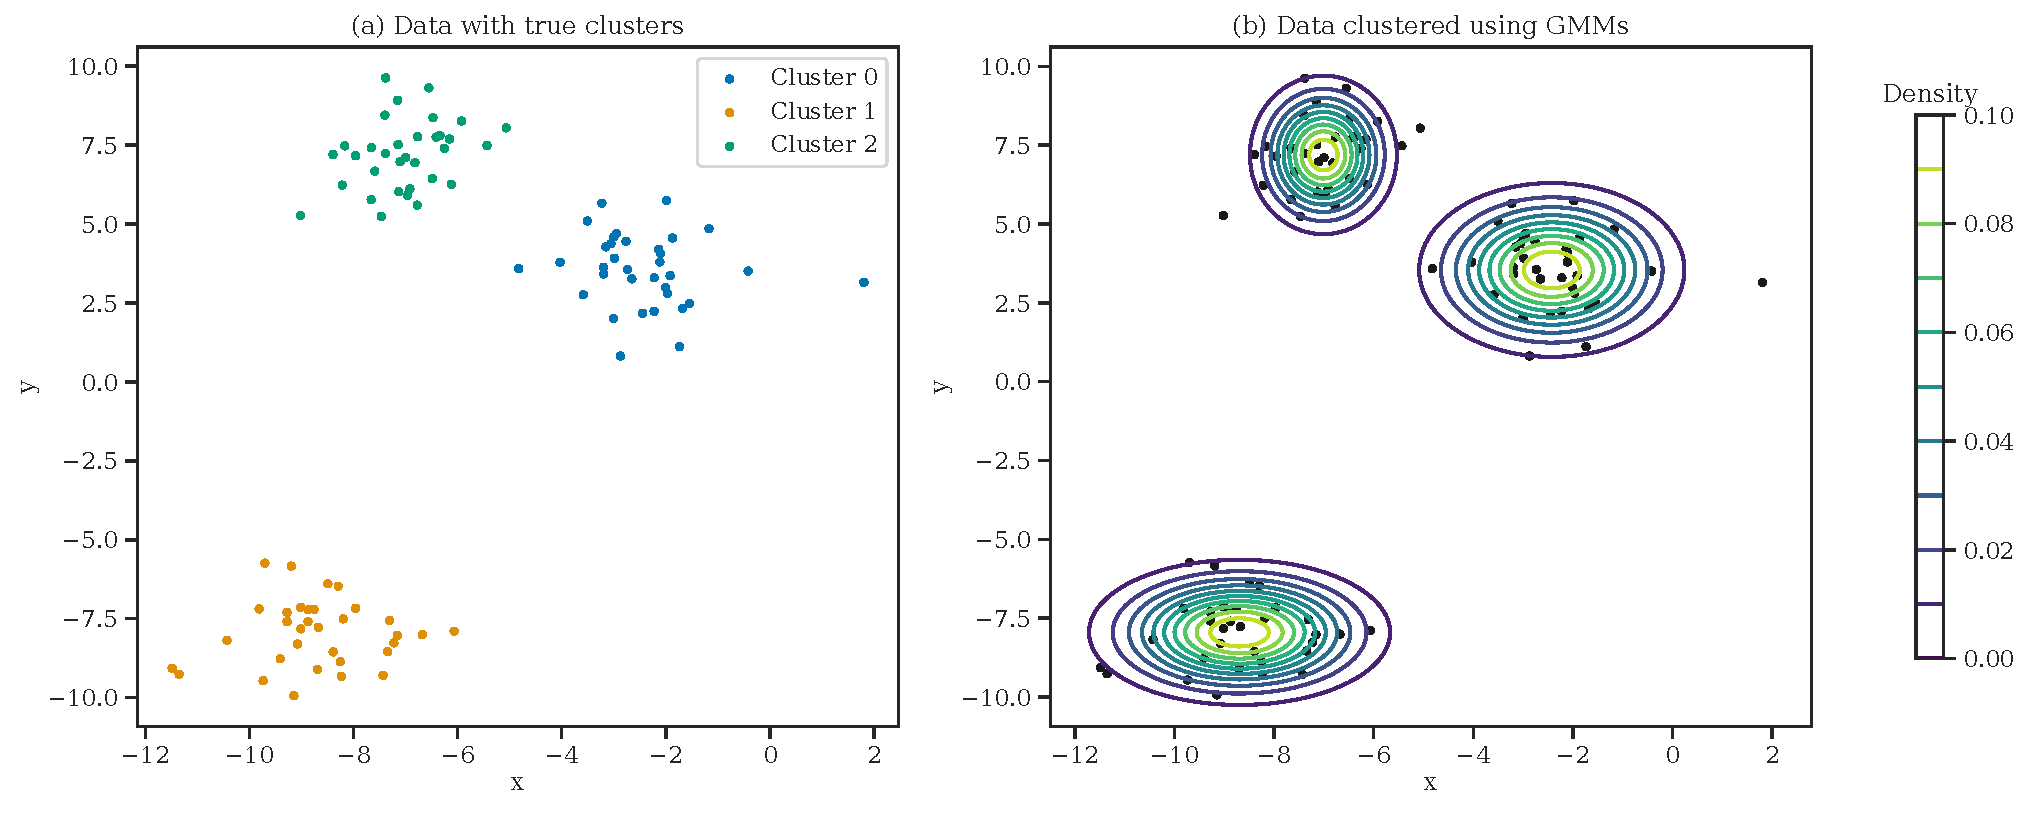
\includegraphics[width=\textwidth]{thesis/figures/k-gmm-clustering-2d-example.pdf}
    \caption{Example of clustering using GMMs on a 2-dimensional data set with 3 clusters. The different clusters have different shapes, as shown by the ellipsoids.}
    \label{fig:k-gmm-clustering-2d-example}
\end{figure}

The main advantage of using GMMs is that clusters can be of different shapes and we get a probabilistic measure of which cluster each data point belongs to (i.e. fuzzy clustering). The convergence time of GMMs depends on the initialization of the parameters $\theta$. If we use k-means clustering to initialize the parameters $\hat{\theta}$, then the overall convergence time is greater than simply running k-means alone. If we use a completely random initialization of the parameters $\theta$, then it converges a lot faster at the risk of converging in a bad local maximum, leading to worse results.

\subsubsection{Hierarchical clustering}
\label{sec:hierarchical-clustering}
\textit{Hierarchical clustering} is a group of clustering algorithms that constructs clusters by recursively partitioning the data points of $X$ in top-down or bottom-up fashion \cite{Rokach2005}. We divide the two methods of hierarchical clustering into what we call \textit{agglomerative} and \textit{divisive hierarchical clustering}. Furthermore, we base this sub-subsection on \cite{Rokach2005}.

Using the agglomerative hierarchical clustering, each data point in $X$ starts in its own cluster and we successively merge them until all points are in their own respective clusters. In contrast to the agglomerative method, divisive hierarchical clustering starts with all data points in $X$ in a single cluster. Then, we divide the single cluster into smaller clusters, until each point is in its own cluster. Following, we call the output of a hierarchical clustering algorithm a \textit{dendrogram}. We use dendrograms to represent the clustering tree structure. We illustrate an example of a dendrogram in \cref{fig:dendrogram-example}.
\begin{figure}[H]
    \centering
    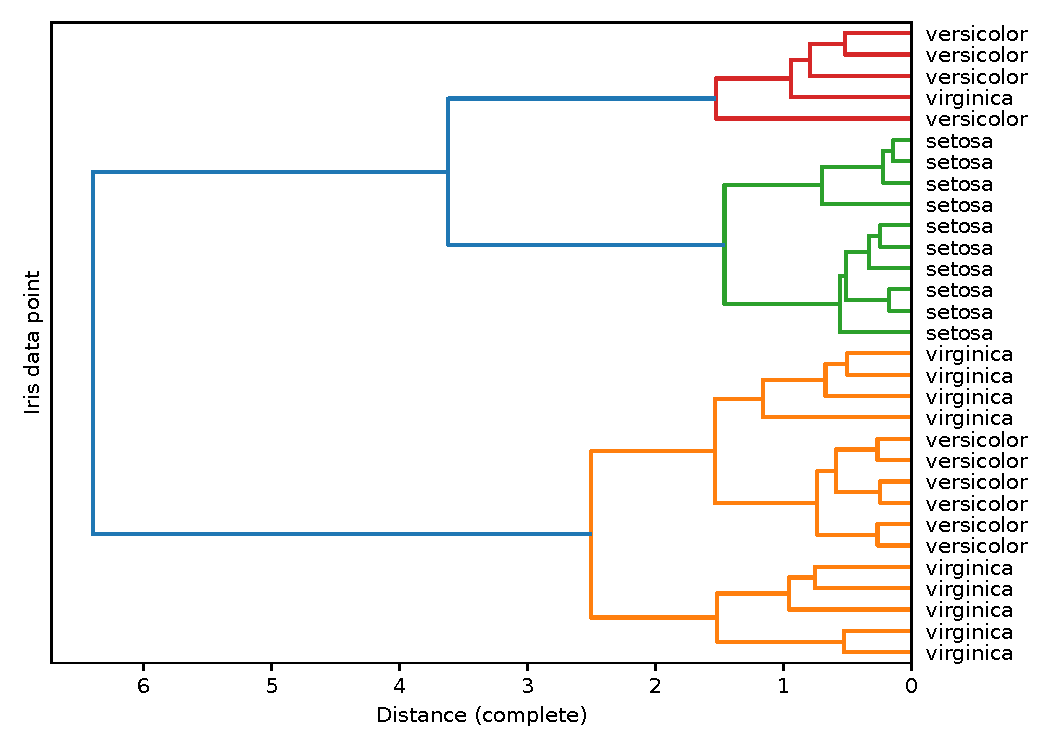
\includegraphics[width=0.9\textwidth]{thesis/figures/dendrogram-example.pdf}
    \caption{Complete-linkage clustering on a subset of the Iris data set \cite{Anderson1936,Fisher1936}, showing its dendrogram.}
    \label{fig:dendrogram-example}
\end{figure}

To merge or divide clusters, we use some similarity measure to either merge similar data points (agglomerative) or divide dissimilar data points (divisive). Exactly which data points we choose to merge or divide depends on which criterion we want to optimize. There exist several different criteria we may choose to perform hierarchical clustering. Below we list some of the most common ones and mention some pros/cons for each criterion.
\begin{itemize}
    \item \textbf{\textit{Single-linkage} clustering} --- combines two clusters that contain the closest pair (i.e. largest similarity) of elements that do not yet belong to the same cluster as each other.
    \begin{itemize}
        \item Single-linkage clustering tends to produce clusters of long chains, which can lead to the clustering of data points which in reality are far apart from each other.
        \item Single-linkage clustering is fast to use for big data sets and can create clusters of different shapes and sizes.
        \item Single-linkage clustering is sensitive to noise.
    \end{itemize}
    \item \textbf{\textit{Complete-linkage} clustering}  --- combines two clusters that contain the furthest pair (i.e. smallest similarity) of elements that do not yet belong to the same cluster as each other.
    \begin{itemize}
        \item Complete-linkage clustering has bias towards spherical clusters.
        \item Complete-linkage clustering works well on data with noise.
        \item Complete-linkage clustering tends to split large clusters.
    \end{itemize}
    \item \textbf{\textit{Average-linkage} clustering} --- combines two clusters such that the average pairwise distance of the new cluster is minimum.
    \begin{itemize}
        \item Average-linkage clustering has bias towards spherical clusters.
        \item Average-linkage clustering works well on data with noise.
    \end{itemize}
    \item \textbf{\textit{Ward-linkage} clustering} --- combines two clusters such that the variance of the new cluster is minimum \cite{Ward1963}.
    \begin{itemize}
        \item Ward-linkage clustering has bias towards spherical clusters.
        \item Ward-linkage clustering works well on data with noise.
    \end{itemize}
\end{itemize}

Overall, hierarchical clustering is a great clustering algorithm for partitioning the data in a tree fashion. By performing hierarchical clustering, we use the resulting dendrogram to determine the number of clusters by cutting it at a certain distance threshold. In the example from \cref{fig:dendrogram-example}, a suitable cut could be at distance equal to 3, leading to 3 clusters. In addition to this, different choices of linkages can lead to very different clusterings. For this reason, we should test multiple linkages to figure out what fits the data the most.

\subsubsection{Spectral clustering}
\label{sec:spectral-clustering}
\textit{Spectral clustering} is a clustering algorithm that first reduces the dimensionality of the data set and then applies a clustering algorithm \cite{Andrew2002}. In particular, spectral clustering uses the eigenvalues of the \textit{affinity matrix} (e.g. a similarity matrix using pairwise Euclidean distances) of the data $X$ to reduce its dimensionality before applying some common clustering algorithm, such as k-means clustering (see \cref{sec:k-means-clustering}). We base this sub-subsection on \cite{Andrew2002}.

Imagine that we want to cluster the data into $k$ clusters. Spectral clustering starts with the construction of the affinity matrix $A$. We typically use some similarity measure to create pairwise distances between data points to create such an affinity matrix. Then, we compute the \textit{graph Laplacian} $L = D - A$, where $D$ is a diagonal matrix with $D_{ii} = \sumlim{j}{} A_{ij}$ and $A$ is the affinity matrix. The graph Laplacian $L$ is simply a matrix representation of a graph, and in our case, the similarities between data points in $X$. Next, we compute the eigenvectors of $L$, and using these eigenvectors we get a lower-dimensional space of the original data $X$ (from $d$ dimensions to $k$). Finally, we use a clustering algorithm, such as k-means clustering, on the eigenvectors of $L$ to get the final clustering.

The main advantage of spectral clustering is that it performs a dimensionality reduction on the data before applying a clustering algorithm. The dimensionality reduction can make the clustering algorithm less prone to noise and yield better results. Unfortunately, the computational requirement of spectral clustering is rather high, and for big data sets, it is simply infeasible.

\subsubsection{HDBSCAN}
\label{sec:hdbscan-clustering}
Clusters come in different shapes and sizes, and real-life data is rather noisy. \textit{DBSCAN} is a density-based algorithm that handles clusters of different shapes and sizes and is robust to noise \cite{Ester1996}. It, however, is only able to produce a "flat" clustering using some global threshold parameter. \textit{HDBSCAN} is a generalization of DBSCAN and improves on it by creating a complete density-based clustering hierarchy \cite{Campello2013}, automatically extracting flat clusters. HDBSCAN is different from the other clustering algorithms we have seen so far, as it can perform clustering without predetermining the number of clusters beforehand and can mark data points a noise. To fully understand the HDBSCAN algorithm, we introduce its key concepts and then explain how the algorithm works in practice. We base this sub-subsection on the "How HDBSCAN Works" article from \cite{how-hdbscan-works-2016}.

HDBSCAN is a density-based clustering algorithm and, for this reason, requires an inexpensive density estimation method to be efficient. Using k-nearest neighbours, the authors of HDBSCAN estimate the density efficiently. In particular, we first define the \textit{core distance} of a data point $x \in X$ to be the distance to the $\textit{minPts}$-nearest neighbour (including $x$), which we denote $d_{core}(x)$. $\textit{minPts}$ is a hyperparameter and controls how conservative we want the clustering to be; the larger $\textit{minPts}$, the more "noisy" data points. To further spread apart data points that have low density, we define the \textit{mutual reachability distance} metric (MRD) as
\begin{align}
    d_{mreach}(x, y) = \max \enclc{ d_{core}(x), d_{core}(y), d(x, y) },
    \label{eqn:mutual_reachability_distance}
\end{align}
where $d(x, y)$ is the distance between data point $x$ and data point $y$ using the original distance metric. Under the MRD metric, data points in dense regions do not change their distances, but for sparse data points, the distances change such that they are at least their core distance to other points.

Next, using the MRD metric, we find dense areas in the data. To find such areas, we create a \textit{minimal spanning tree} (MST) where each node represents a data point $x \in X$ and edges connecting pairs of nodes has a weight equal to the MRD between the two nodes. By using an MST, we get a graph with the minimal set of edges between nodes such that the weight between the nodes is minimal. Additionally, if we drop exactly one edge of the graph, we disconnect it; for each pair of nodes, we connect them by exactly one edge. Using these two facts, we create a clustering hierarchy in a single-linkage clustering manner. First, we sort the weights of the edges of the MST in increasing order. Following, we iterate over the edges of the MST and merge data points into clusters (note that each data point is its own cluster initially). Now, from the hierarchical clustering, we are left with a dendrogram, which we illustrate in \cref{fig:hdbscan-dendrogram-example}. We are now are left with a critical question: How should we define the cut to get a flat clustering?
\begin{figure}[H]
    \centering
    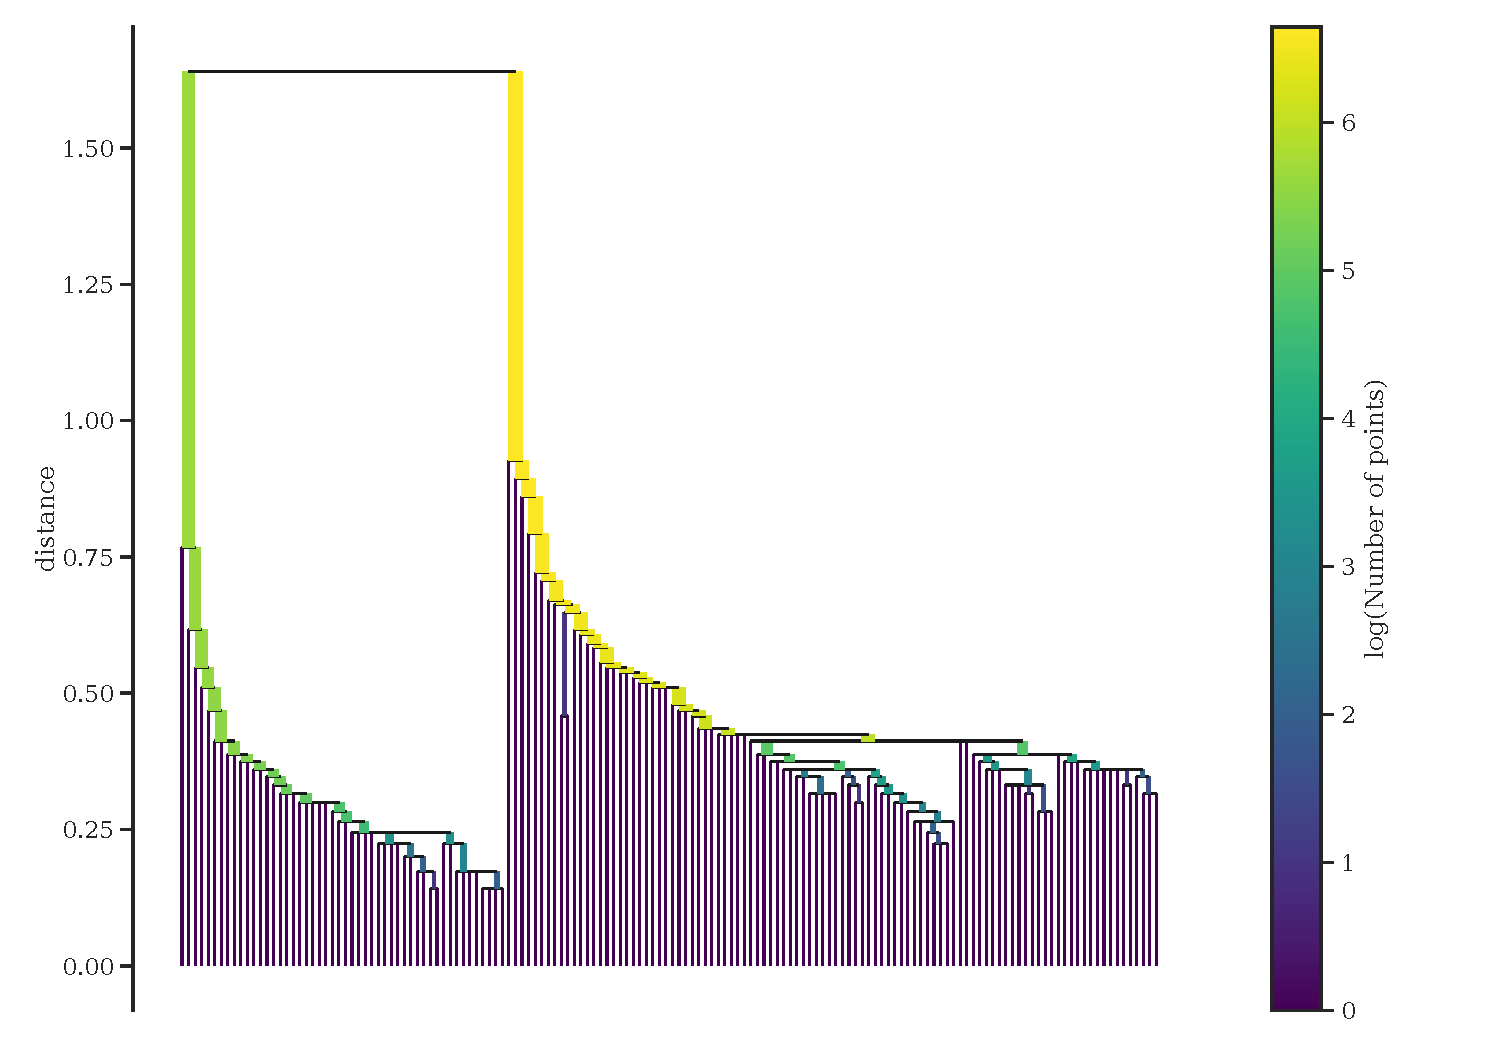
\includegraphics[width=0.8\textwidth]{thesis/figures/hdbscan-single-linage-tree-example.pdf}
    \caption{Single-linkage dendrogram plot from HDBSCAN on the Iris data set \cite{Anderson1936,Fisher1936}.}
    \label{fig:hdbscan-dendrogram-example}
\end{figure}

Dendrograms can be very difficult to interpret, especially once we reach a certain number of data points. For this reason, the authors of HDBSCAN condense (or compact) the dendrogram from the hierarchical clustering such that they obtain a flat clustering. First, we define the notion of \textit{minClusterSize}, which is a hyperparameter controlling the minimal cluster size at any time. Following, we walk down the dendrogram, starting from the root cluster, and at each split, we check whether or not the new cluster has at least \textit{minClusterSize} data points in it. If the new cluster has at least \textit{minClusterSize} data points in it, we let that cluster be in the tree. If the new cluster has less than the \textit{minClusterSize} in it, then we let the parent cluster identify the new cluster and we remove the node from the tree. As we walk through the dendrogram to condense it, we also include at what distance clusters merge into the parent cluster, i.e. "fall out of clusters". We illustrate with an example of a condensed dendrogram in \cref{fig:hdbscan-condensed-dendrogram-example}.
\begin{figure}[H]
    \centering
    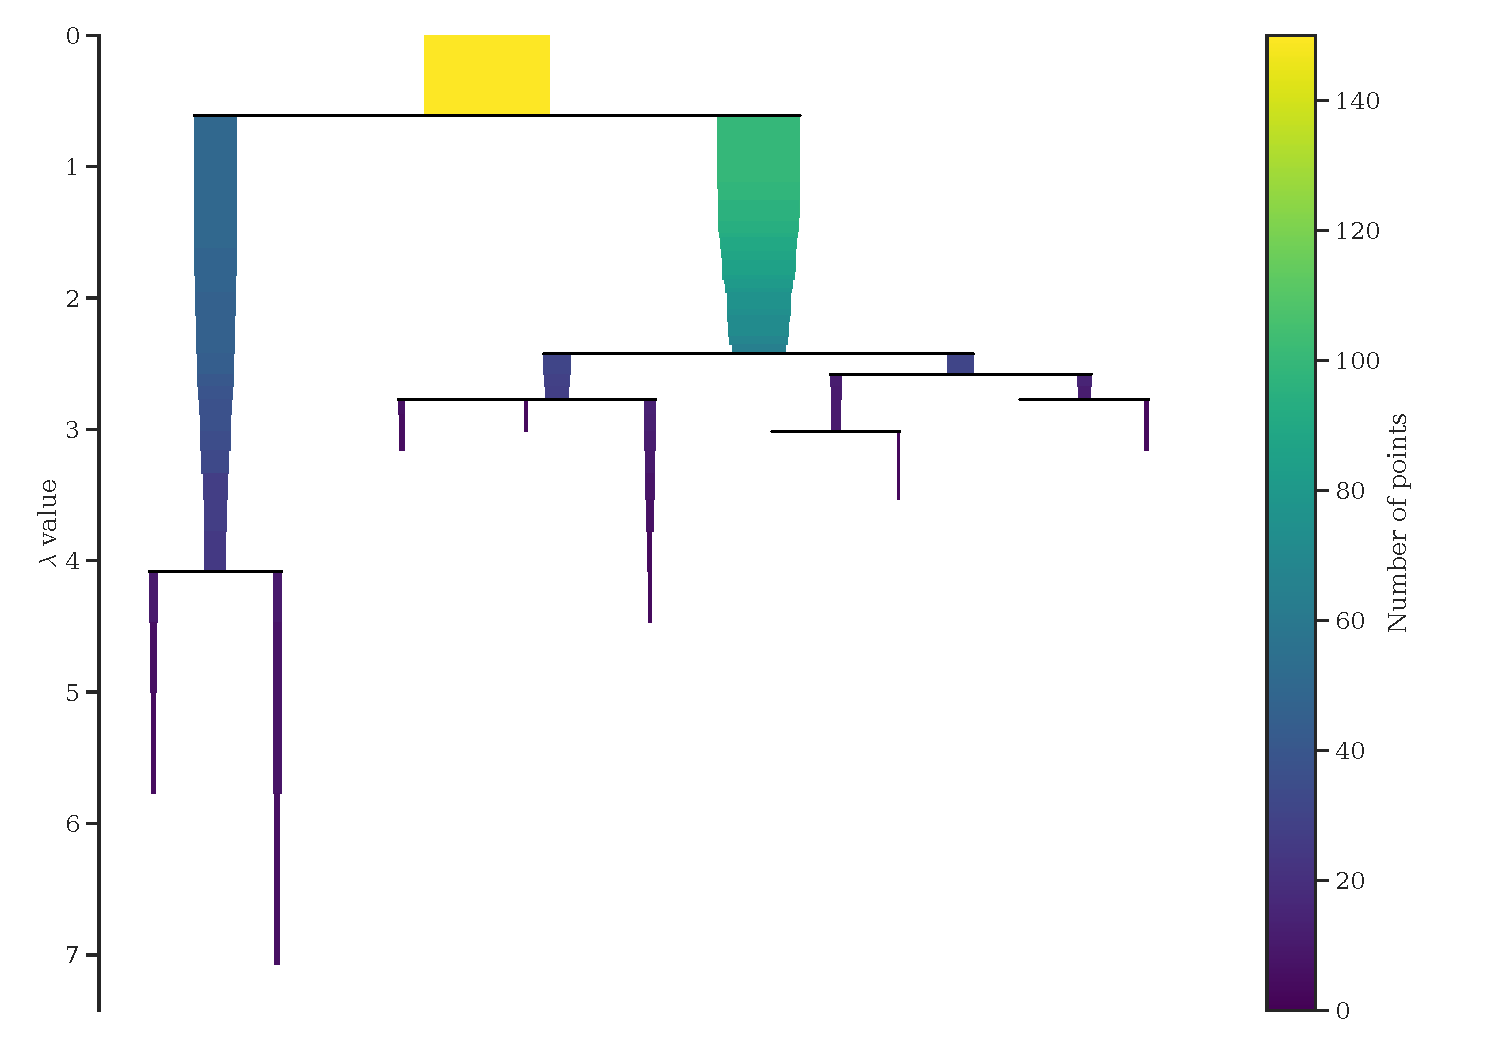
\includegraphics[width=0.8\textwidth]{thesis/figures/hdbscan-condensed-tree-example.pdf}
    \caption{Condensed dendrogram plot from HDBSCAN on the Iris data set \cite{Anderson1936,Fisher1936}.}
    \label{fig:hdbscan-condensed-dendrogram-example}
\end{figure}

Now, to define the flat cut in a condensed diagram, we select the clusters such that the largest total area of "ink" is maximal, under an additional constraint that we do not select clusters that are descendants of an already selected cluster. Furthermore, we mark any clusters which we do not select in the previous step as noise, as they are merely artefacts of the initial hierarchical clustering. We then decide the final clustering, which we illustrate in \cref{fig:hdbscan-condensed-dendrogram-final-cut-example}.
\begin{figure}[H]
    \centering
    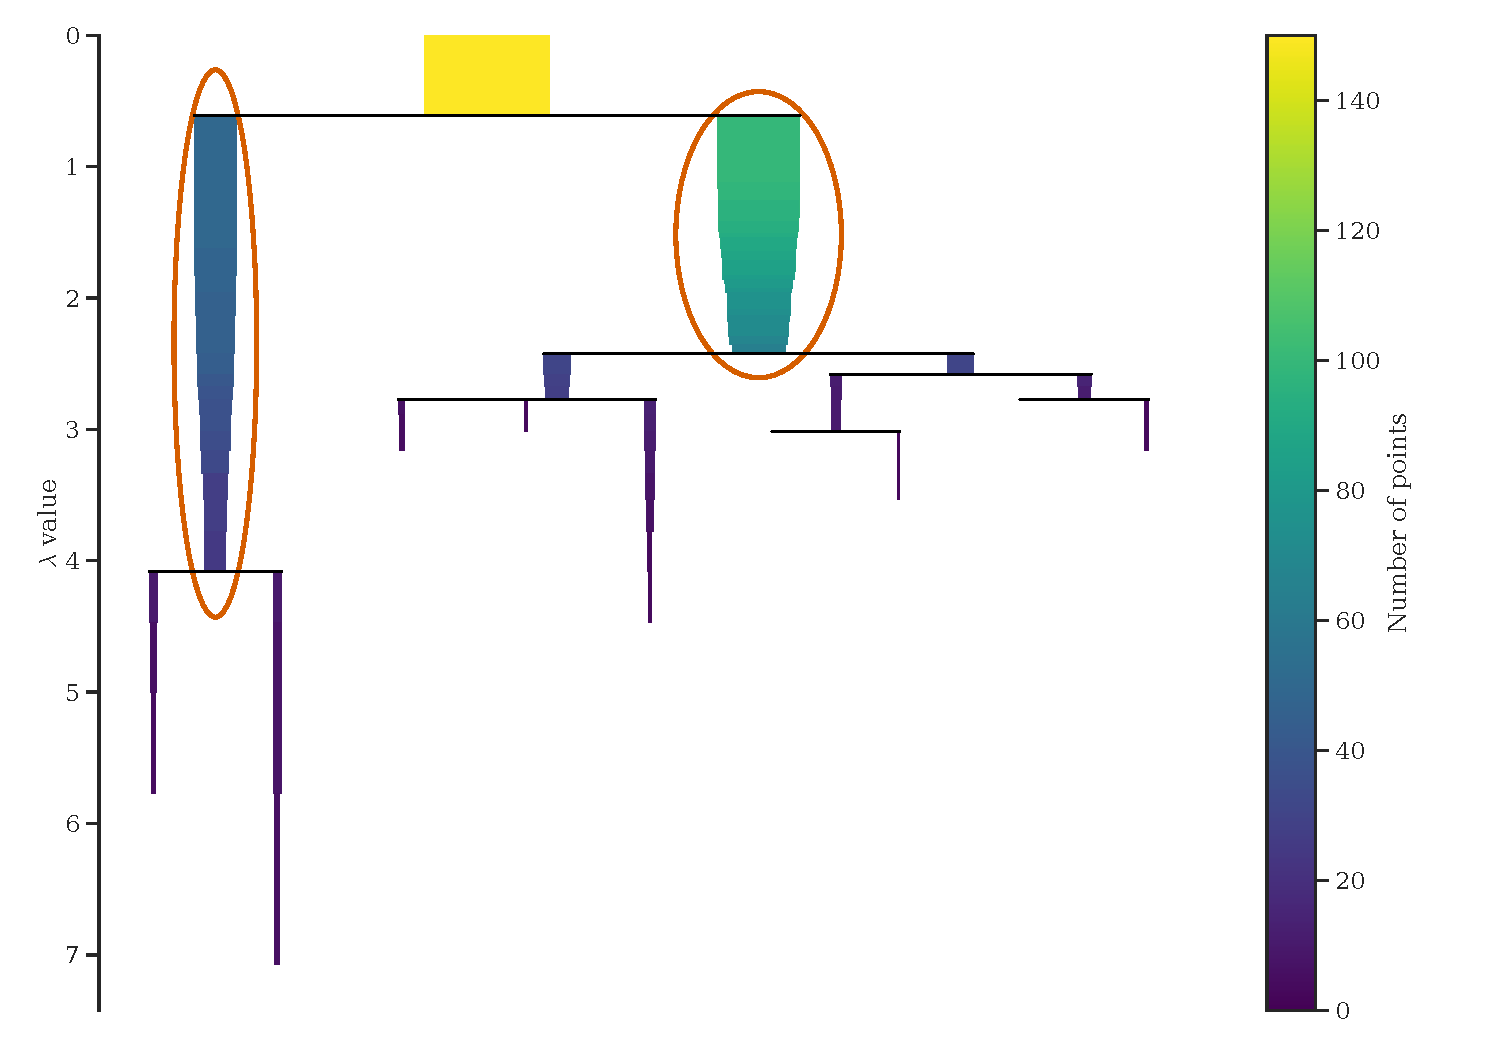
\includegraphics[width=0.8\textwidth]{thesis/figures/hdbscan-condensed-tree-final-cut-example.pdf}
    \caption{Condensed dendrogram plot from HDBSCAN on the Iris data set \cite{Anderson1936,Fisher1936}. We show the "final cut" in the red circles and consider all data points below the clusters with the red circles as noise.}
    \label{fig:hdbscan-condensed-dendrogram-final-cut-example}
\end{figure}

The main advantage of HDBSCAN is that it is able to find the number of clusters automatically, that we can have different shapes of clusters and are able to mark data points as noise. Dealing with noisy data points can be a challenge, and depending on how we treat them (exclusion, each noisy data point in its own cluster, etc.), it may lead to very different results.

\subsubsection{ToMATo}
\label{sec:tomato-clustering}
\textit{Topological Mode Analysis Tool} (ToMATo) is a clustering algorithm that uses concepts from topological data analysis (TDA) \cite[p. 118-131]{Oudot2015}. In particular, ToMATo uses the concepts of persistence diagrams (see \cref{sec:persistence diagram}) and prominence to perform clustering. We divide the ToMATo clustering algorithm into three parts: density estimation and neighbour graph creation (1), mode-seeking (2) and merging (3). Furthermore, we refer to \cite[p. 118-131]{Oudot2015} when explaining the algorithm.

First (1), we use any density estimation scheme to estimate the density of our data. A common choice is to use kernel density estimation with some kernel (e.g. Gaussian). We denote the density of a data point $x_i \in X, i = 1, 2, \ldots, n$ as $\Tilde{f}(x_i)$. In addition to density estimation, we compute a neighbourhood graph $G$ to determine the neighbours of data points. In the graph $G$, each vertex is a data point and edges represent neighbours. To compute $G$, it is common to use a $k$-nearest neighbour graph, where $k$ represents the number of neighbours.

Using the density estimator $\Tilde{f}$ and neighbourhood graph $G$, we compute the initial clusters of ToMATo by performing mode-seeking (2). First, we sort the vertices of $G$ by decreasing $\Tilde{f}$-values and iterate over them. At each vertex $i$, compare the $\Tilde{f}$ values of vertex $i$ and its neighbours. If $\Tilde{f}(x_i)$ is greater than $\Tilde{f}$ of its neighbours, we then denote vertex $i$ as a peak of $\Tilde{f}$. Otherwise, we connect vertex $i$ to the neighbour with the greatest $\Tilde{f}$-value. By doing so, we create a spanning forest, where each spanning tree represents peaks of the underlying true density function. In the next step, we use this spanning forest and merge the trees to obtain a clustering.

The last step is the merging (3) of the spanning forest from (2). To do this, ToMATo iterates over the vertices of $G$ again (in the same order as in (2)) and we use a \textit{union-find} data structure to keep track of the spanning trees we merge. We denote the union-find data structure as $\mathcal{U}$. The entries $e \in \mathcal{U}$ correspond to the union of spanning trees. The root of an entry $r(e)$, is the vertex in $e$ whose $\Tilde{f}$-value is the highest, i.e. a local peak of $\Tilde{f}$ in $G$. Now, iterating over the vertices of $G$, we check whether or not vertex $i$ is a peak of $\Tilde{f}$. If vertex $i$ is a peak of $\Tilde{f}$, i.e. root of some spanning tree $S$, we create a new entry $e$ in $\mathcal{U}$, in which we store $S$. The root of entry $e$ is set to the vertex itself, i.e. $r(e) = i$. If vertex $i$ is not a peak of $\Tilde{f}$, it means that it belongs to some existing entry $e_i \in \mathcal{U}$ and we look for potential merges of $e_i$ with other entries in $\mathcal{U}$. In particular, we iterate over neighbours $e \in \mathcal{E}$, $e \neq e_i$, of $i$ in $G$ and check whether $\min \enclc{ \Tilde{f}(x_{r(e)}), \Tilde{f}(x_{r(e_i)}) } < \Tilde{f}(x_i) + \tau$, where $\tau$ is the \textit{prominence} threshold parameter. In other words, we check whether or not two entries have different $\Tilde{f}$-value and at least one of them has root with less than $\tau$ prominence. If this is true, we merge $e$ and $e_i$ into a single entry in $\mathcal{U}$, i.e. $e \cup e_i$, and we merge the entry with the lower root into the one with the higher root.

Once the merging step is complete, we are left with a union-find structure $\mathcal{U}$. For every entry $e$ of $\mathcal{U}$, we connect them to its parent entry $p(e)$ such that $\Tilde{f}(x_{p(e)}) > \Tilde{f}(x_e)$. In other words, by iteratively searching for the topmost parent, we determine which cluster we connect each entry (i.e. data point) to. We see the ToMATo clustering algorithm as a combination of mode-seeking (from step (2)) and hierarchical clustering (from step (3)). As a result of the hierarchical structure, we can visualize when entries in $\mathcal{U}$ merge into other entries, and thus, explain the lifespans of entries. More precisely, an entry in $\mathcal{U}$ is "born" when we create it in $\mathcal{U}$ and "dies" when we merge it into another entry with a higher root. Using persistence diagrams (see \cref{sec:persistence diagram}) we can explain the lifespans of entries and determine which entries live the longest (i.e. entries that never dies). We use the persistence diagram to determine which value for $\tau$ we should use. Different values of $\tau$ results in different numbers of clusters. In practice, let $\tau = +\inf$ and use the persistence diagram of $\mathcal{U}$ to find a suitable threshold $\hat{\tau}$ such that we get the number of clusters we want. Then, we run ToMATo again using $\hat{\tau}$ as the threshold parameter to get the final clustering. Finally, we motivate the use of ToMATo in \cref{fig:k-tomato-clustering-2d-example}, where we see from the persistence diagram in (b) that ToMATo found 5 clusters, but 3 of them are significantly far from the diagonal (i.e. high prominence). This indicates that the data set should consist of 3 clusters, and thus, we run ToMATo again setting the prominence threshold such that we get 3 clusters.
\begin{figure}[H]
    \centering
    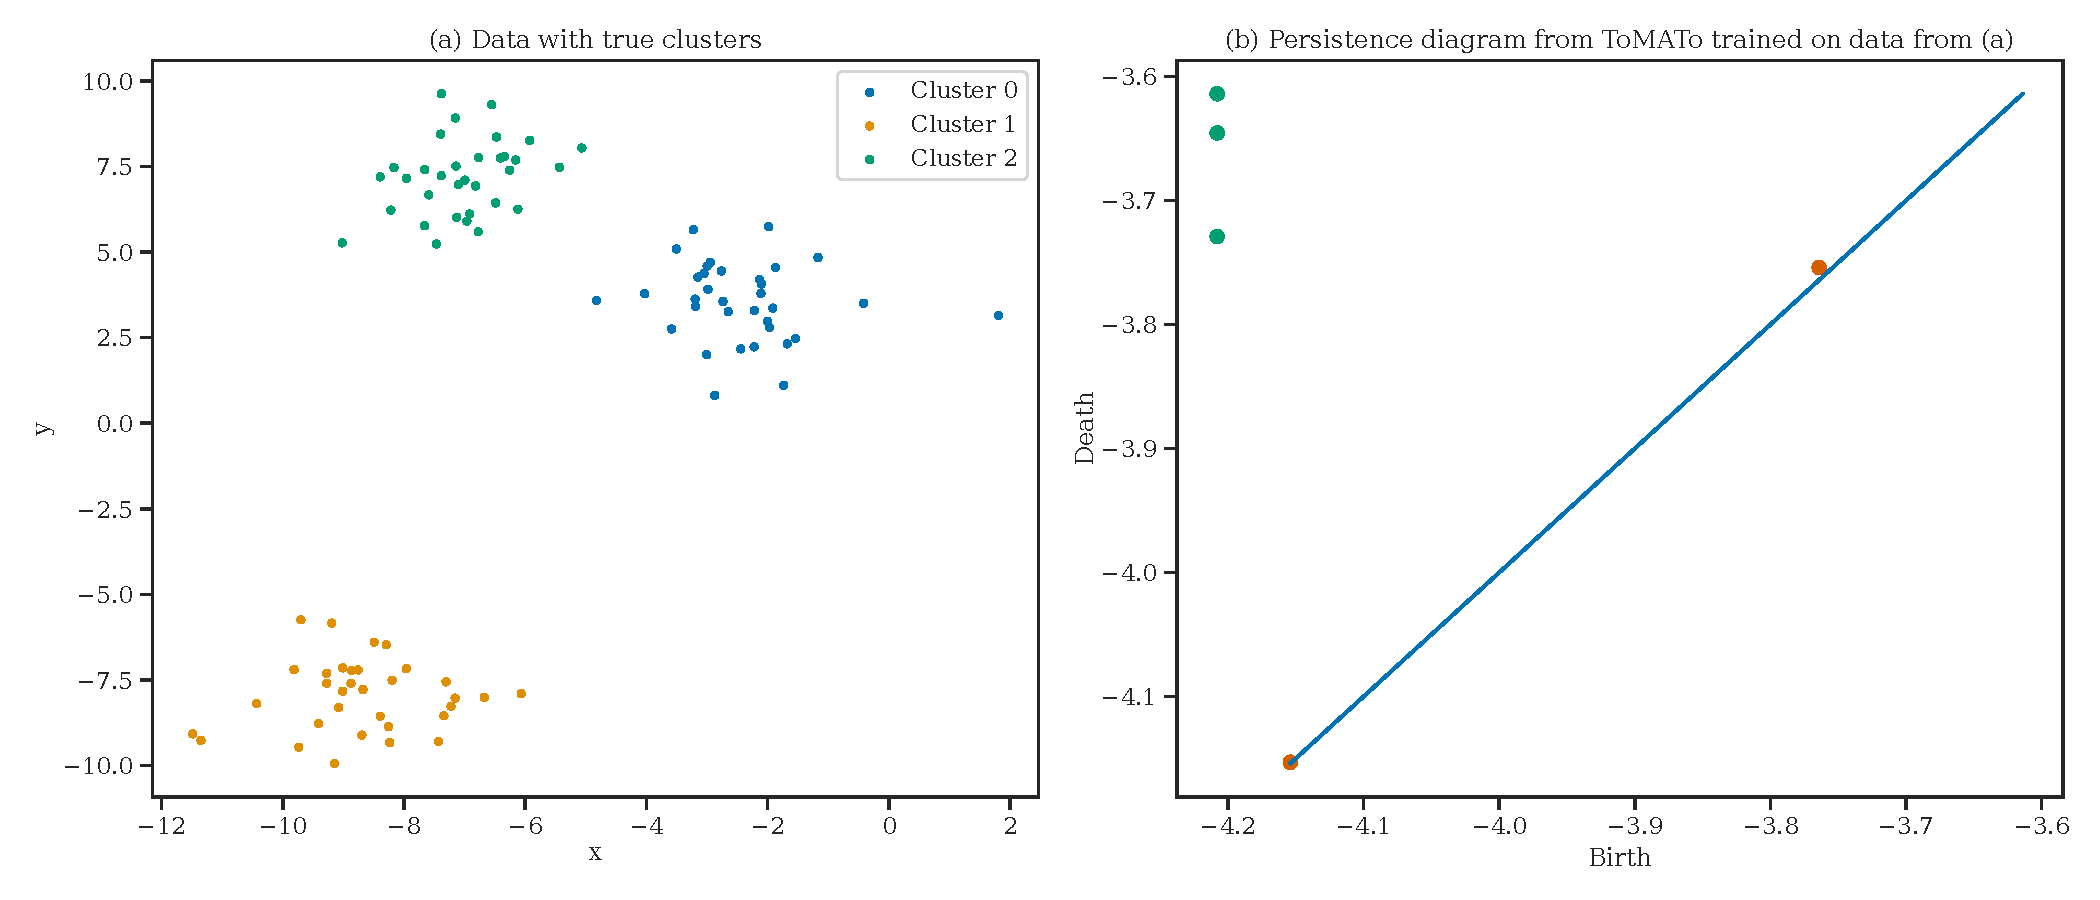
\includegraphics[width=\textwidth]{thesis/figures/k-tomato-clustering-2d-example.pdf}
    \caption{Example of clustering using ToMATo on a 2-dimensional data set with 3 clusters. The persistence diagram in (b) shows the three prominent clusters (green dots).}
    \label{fig:k-tomato-clustering-2d-example}
\end{figure}

What is great about ToMATo is that it gives us a way to determine the numbers of clusters automatically (e.g. using some heuristic on the first persistence diagram to determine $\hat{\tau}$). In addition to this, ToMATo works with any metric, as long as we can create a neighbourhood graph (e.g. using Euclidean distance or similar metrics).

\subsubsection{Comparison of clustering algorithms}
\label{sec:comparison-of-clustering-algorithms}
In \cref{sec:clustering-algorithms}, we describe several algorithms for clustering data. We tabularize the strengths and weaknesses for each algorithm in \cref{table:clustering-algorithms-comparison}. Even though some algorithms might tick off more properties than others, it does not mean that it is a perfect algorithm for all types of data sets. In particular, we have to perform cluster validation to evaluate the results from various cluster algorithms to figure out what algorithm works the best. We explain how to validate results from cluster algorithms in \cref{sec:cluster-validation}.
\begin{table}[H]
    \centering
    \begin{tabular}{@{}lcccccccc@{}}
    \toprule
        & \multicolumn{8}{c}{Algorithm} \\ \cmidrule(l){2-9} 
        \multicolumn{1}{c}{Property} & \multicolumn{1}{l}{\rot{k-means}} & \multicolumn{1}{l}{\rot{MB k-means}} & \multicolumn{1}{l}{\rot{k-medoids}} & \multicolumn{1}{l}{\rot{GMMs}} & \multicolumn{1}{l}{\rot{Hierarchical}} & \multicolumn{1}{l}{\rot{Spectral}} & \multicolumn{1}{l}{\rot{HDBSCAN}} & \multicolumn{1}{l}{\rot{ToMATo}} \\ \midrule
        \trcolor Practical for large data sets & \xmark & \xmark & & \xmark & \xmark & & \xmark & \xmark \\
        Determining the number of clusters automatically & & & & & \xmark & & \xmark & \xmark \\
        \trcolor Cluster centroids as data points & & & \xmark & & & & & \\
        Different clusters shapes & & & & \xmark & \xmark & & \xmark & \xmark \\
        \trcolor Hierarchical clustering & & & & & \xmark & & \xmark & \\
        Robust against nosy data sets & & & \xmark & & & \xmark & \xmark & \xmark \\
        \trcolor Can identify noisy/anomalous data points & & & & & & & \xmark & \xmark \\
        User-defined distance metric & & & \xmark & & \xmark & \xmark & \xmark & \xmark \\ \bottomrule
    \end{tabular}
    \caption{Comparison of various properties for each clustering algorithm we describe in \cref{sec:clustering-algorithms}.}
    \label{table:clustering-algorithms-comparison}
\end{table}

\subsection{Cluster validation}
\label{sec:cluster-validation}
After we use clustering algorithms to perform clustering, we evaluate the result to find the best set of hyperparameters and/or clustering algorithm. This raises the question: which clustering algorithm performs the best on our data? Thankfully, there exist a handful of various methods to tackle this task. In particular, we differentiate between \textit{internal} and \textit{external cluster validation algorithms}. Internal cluster validation algorithms assess the performance of the clustering using statistics of the data, without knowing the true labels at hand. External cluster validation algorithms, on the other hand, use the knowledge of the true labels. In this thesis, we only use internal cluster validation algorithms, as we are mostly working with data where we do not know the labels beforehand. Recall that, in most clustering algorithms, we want the average distance between any two data points in the same cluster to be as small as possible (compactness); and the average distance between any two data points from different clusters to be as large as possible (separation). Internal cluster validation algorithms usually reflect compactness or separation of clusterings. In the next sub-subsections, we explain some common choices of internal cluster validation algorithms and discuss their strengths and weaknesses. Furthermore, we will use the cluster validation methods we explain below when we analyze word embeddings (\cref{sec:word-embeddings}) in \cref{chap:analysis-of-word-embeddings}.

\subsubsection{Silhouette Coefficient}
\label{sec:silhouette-coefficient}
The \textit{Silhouette Coefficient} is an internal cluster validation method that measures the goodness of clusterings \cite[p. 87]{Kaufman1990}. In particular, the Silhouette Coefficient measures how similar data points are to their own cluster (compactness) when we compare to data points from other clusters (separation). The Silhouette Coefficient ranges from -1 to 1, where the best value is 1 and the worst value is -1. Values near 0 indicate that we have overlapping clusters (i.e. low separation). We base this sub-subsection on \cite[p. 87]{Kaufman1990}.

For any data point $x_i$ in the cluster $C_i$, we compute the mean compactness $a(i)$ as the average distance $d(i, j)$ between data point $i$ and all other data points in $C_i$, i.e. $j \in C_i, i \neq j$. More formally, we define the mean compactness $a(i)$ as
\begin{align}
    a(i) = \frac{1}{|C_i| - 1} \sumlim{j \in C_i, i \neq j}{}{d(i, j)},
    \label{eqn:silhouette-coef-a}
\end{align}
where $|C_i|$ is the number of data points in cluster $C_i$. Smaller values of $a(i)$ indicate better compactness of clusters, and thus, better cluster assignments. Following, for any data point $x_i$ in the cluster $C_i$, we compute the mean separation $b(i)$ as the smallest distance from $i$ to any other cluster in which $i$ does not belong. The mean separation $b(i)$ is defined as
\begin{align}
    b(i) = \min_{k \neq i} \frac{1}{|C_k|} \sumlim{j \in C_k}{}{d(i, j)}.
    \label{eqn:silhouette-coef-b}
\end{align}
Large values of $b(i)$ indicate that the clusters have good separation and that data points in $C_i$ are a good fit. Now, using the definitions of compactness and separation, we define the \textit{silhouette} of data point $i$ as
\begin{align}
    s(i) = \begin{cases}
        \frac{b(i) - a(i)}{\max \enclp{a(i), b(i)}} & \mbox{if } |C_i| > 1 \\
        0 & \mbox{if } |C_i| = 1
    \end{cases}.
\end{align}
Taking the average of all silhouettes $s(i)$, we define the \textit{mean Silhouette Coefficient} as
\begin{align}
    SC = \frac{1}{n} \sumlim{i=1}{n}{s(i)},
    \label{eqn:silhouette-coef}
\end{align}
where $n$ is the number of data points in our data (e.g. $n$-dimensional data $X$).

The main advantages of the mean Silhouette Coefficient are that it is simple, fast to compute and has a defined range from -1 to 1. The mean Silhouette Coefficient struggles with overlapping clusters (where $SC \approx 0$).

\subsubsection{Davies-Bouldin Index}
\label{sec:davies-bouldin-index}
The \textit{Davies-Bouldin Index} (DBI) is an internal cluster validation method for evaluating results of clustering algorithms \cite{DaviesBouldin1979}. Similar to the Silhouette Coefficient, DBI measures the compactness and separation of clusters to measure the goodness of fit. We base this sub-subsection on \cite{DaviesBouldin1979}.

To measure the compactness of clusters, DBI introduces the notion of \textit{scatter within a cluster}, which we denote $S_i$. We compute $S_i$ by taking the mean of the sum of the distances to the cluster centroid of a particular data point $i$. More formally, we define $S_i$ as
\begin{align}
    S_i = \enclp{ \frac{1}{|C_i|} \sumlim{x_j \in C_i}{} |x_j - \Tilde{C_i}|^p}^{1/p},
    \label{eqn:dbi-s}
\end{align}
where $C_i$ is the cluster we associate to data point $i$, $|C_i|$ is the number of data points in cluster $C_i$, $\Tilde{C_i}$ is the centroid of cluster $C_i$ and $p$ denotes the power of the $L^p$ distance. A common choice is to set $p=2$, leading to Euclidean distances. A low value of $S_i$ indicates that the compactness of cluster $C_i$ is good. To compute the separation of clusters, DBI computes separation between clusters $C_i$ and $C_j$ by taking the distance between cluster centroids $\Tilde{C_i}$ and $\Tilde{C_j}$. We define the cluster separation $M_{i, j}$ as
\begin{align}
    M_{i, j} = ||\Tilde{C_i} - \Tilde{C_j}||_p,
    \label{eqn:dbi-m}
\end{align}
where $p$ denotes the power of the $L^p$ distance. High values of $M_{i, j}$ indicate that we separate the clusters well. Combining the notion of cluster compactness $S_i$ and separation $M_{i, j}$, we define the measure of cluster goodness $R_{i, j}$ as
\begin{align}
    R_{i, j} = \frac{S_i + S_j}{M_{i, j}}.
    \label{eqn:dbi-r}
\end{align}
To create a clustering measure that is symmetric and non-negative, we define $R_{i, j}$ as such. Low values of $R_{i, j}$ indicate that we have compact clusters with high separation. For a particular cluster $C_i$, DBI measures $R_{i, j}$ for all other clusters $C_j$, $j \neq i$, and uses the largest value of $R_{i, j}$, i.e. the worst-case scenario to compute the index. More formally, we define DBI as
\begin{align}
    DBI = \frac{1}{n} \sumlim{i=1}{n} \max_{j \neq i} R_{i, j},
    \label{eqn:dbi}
\end{align}
where $n$ is the number of data points in our data (e.g. $n$-dimensional data $X$). The main advantage of DBI is the fact that is fast to compute and has non-negative values. Since DBI does not have any upper bound, it is more difficult to interpret the values, when we for instance compare it to Silhouette Coefficient.

\subsubsection{Caliński-Harabasz Index}
\label{sec:calinski-harabasz-index}
The \textit{Caliński-Harabasz Index} (CHI) is an internal cluster validation method for evaluating clustering algorithms \cite{CalinskiHarabasz1974}. CHI measures compactness and separation of clusters to measure the goodness of fit of a particular clustering. We base this sub-subsection on \cite{CalinskiHarabasz1974}.

To measure the compactness of a clustering, CHI computes the \textit{sum-of-squares within cluster} (SSW) as
\begin{align}
    SSW = \sumlim{i=1}{n} ||x_i - \Tilde{C_i}||^2,
    \label{eqn:chi-ssw}
\end{align}
where $n$ is the number of data points in our data, $x_i$ is the $i$th data point and $\Tilde{C_i}$ is the centroid of the cluster we associate to $x_i$. Small values of SSW indicate that we have compactly clustered data points. To measure the separation of clusters, CHI computes the \textit{sum-of-squares between clusters} (SSB) as
\begin{align}
    SSB = \sumlim{j=1}{k} |C_j| \cdot ||\Tilde{C_i} - \Bar{X}||^2,
    \label{eqn:chi-ssb}
\end{align}
where $k$ is the number of clusters, $|C_j|$ is the number of data points in cluster $C_j$ and $\overline{X}$ is the centre of all data points (i.e. mean). Large values of SSB indicate that we have a good separation of the clusters. Finally, we compute the CHI by multiplying the ratio of SSB to SSW with a weight depending on $n$ and $k$. More formally, the CHI is defined as
\begin{align}
    CHI = \frac{SSB}{SSW} \times \frac{n - k}{k - 1}.
    \label{eqn:chi}
\end{align}
Since we define CHI as the ratio between SSB and SSW, large values indicate better clustering. The main advantage of CHI is that it is fast to compute. Similar to Davies-Boundin Index, CHI is harder to interpret than Silhouette Coefficient for example, since the values do not have any upper limit.

\subsection{Dimensionality reduction methods}
\label{sec:dimensionality-reduction-methods}
Working with data in high dimensions can be a difficult task. Imagine that we have gathered some data, containing several features, and we would like to deepen our understanding of it. One approach we could do would be to visualize each feature by plotting them against each other, looking for bivariate relationships. Unfortunately, this is a rather cumbersome task and is hard to employ once a certain number of features is met (e.g. 10 features). Thankfully, \textit{dimensionality reduction methods} can help us to reduce the dimensionality of data into some lower dimension, preserving relevant properties of the original data in the process. A typical application of dimensionality reduction methods is to lower the dimensionality to 2 or 3 such that we can visualize the data at ease. We introduce two dimensionality reduction methods and explain how they work. In both sub-subsections below, we assume that we have some data $X \in \R^{n \times d}$ and that we want to reduce the dimensionality to some chosen hyperparameter $k$. Furthermore, we will use the dimensionality reduction methods which we explain below when we analyse clustering of word embeddings (\cref{sec:word-embeddings}) in \cref{chap:analysis-of-word-embeddings} and prediction of polysemous words in \cref{sec:analysis-of-embeddings-supervised-polysemy-prediction}.

\subsubsection{Principal Component Analysis}
\label{sec:pca}
\textit{Principal Component Analysis} (PCA) is one of the most common dimensionality reduction methods \cite{Jolliffe2002}. PCA performs a linear mapping of the original data $X \in \R^{n \times d}$ to a (possibly) lower-dimensional space $Y \in \R^{n \times k}$ ($k \leq d$) such that the variance is maximal in $Y$. We typically select $k$ to be a relatively low value, e.g. 2 or 3, if we would like to visualize it using plots. Another common value for $k$ is to set it such that a specific variance threshold is met, e.g. explaining 90\% of the variance of the data. We refer to \cite{Jolliffe2002} when explaining PCA.

The PCA algorithm consists of several steps, and following, we explain each step. First, compute the mean of $X$, which we denote $\overline{X} = \frac{1}{n} \sumlim{i=1}{n} x_i$, and subtract it from $X$, i.e. $X' = X - \overline{X} = \enclc{x'_1, x'_2, \ldots, x'_n}$. Next, we compute the covariance matrix of $X'$, which we denote $C \in \R^{d \times d}$, and we compute the corresponding eigenvectors and eigenvalues of $C$, which we denote $C_\text{eig} = \enclc{c_1, c_2, \ldots, c_d}$. Furthermore, we sort the eigenvectors $C_\text{eig}$ by its corresponding eigenvalues in a descending manner. By doing so, we get a set of eigenvectors such that the first eigenvector corresponds with the largest value, the second eigenvector corresponds with the second largest value and so forth. We denote this set of eigenvectors as $C'_\text{eig} = \enclc{c'_1, c'_2, \ldots, c'_d}$. We then pick the $k$ first eigenvectors of $C'_\text{eig}$ and project the data onto them, essentially performing a \textit{change of basis}. In addition to this, we add the mean of $X$ to complete the reconstruction. We define the reconstruction of PCA as
\begin{align}
    Y = X' \trans{\begin{pmatrix}
    c'_1 & c'_2 & \ldots & c'_k
    \end{pmatrix}} + \overline{X},
    \label{eqn:pca-projection}
\end{align}
where $Y = \enclc{y_1, y_2, \ldots, y_n}$ represents the original data $X$ in (a possibly) lower dimension $k$, such that we maximize the variance of the vectors of $X$. We refer the vectors $\enclc{y_1, y_2, \ldots, y_n}$ as the principal components (PC) of $X$, where PC1 is $y_1$, PC2 is $y_2$ and so forth. Finally, we show an example where we apply PCA to some 2-dimensional data in \cref{fig:pca-2d-example}, where we see that PCA essentially rotates the data, maximizing the variance in the PC axes.
\begin{figure}[H]
    \centering
    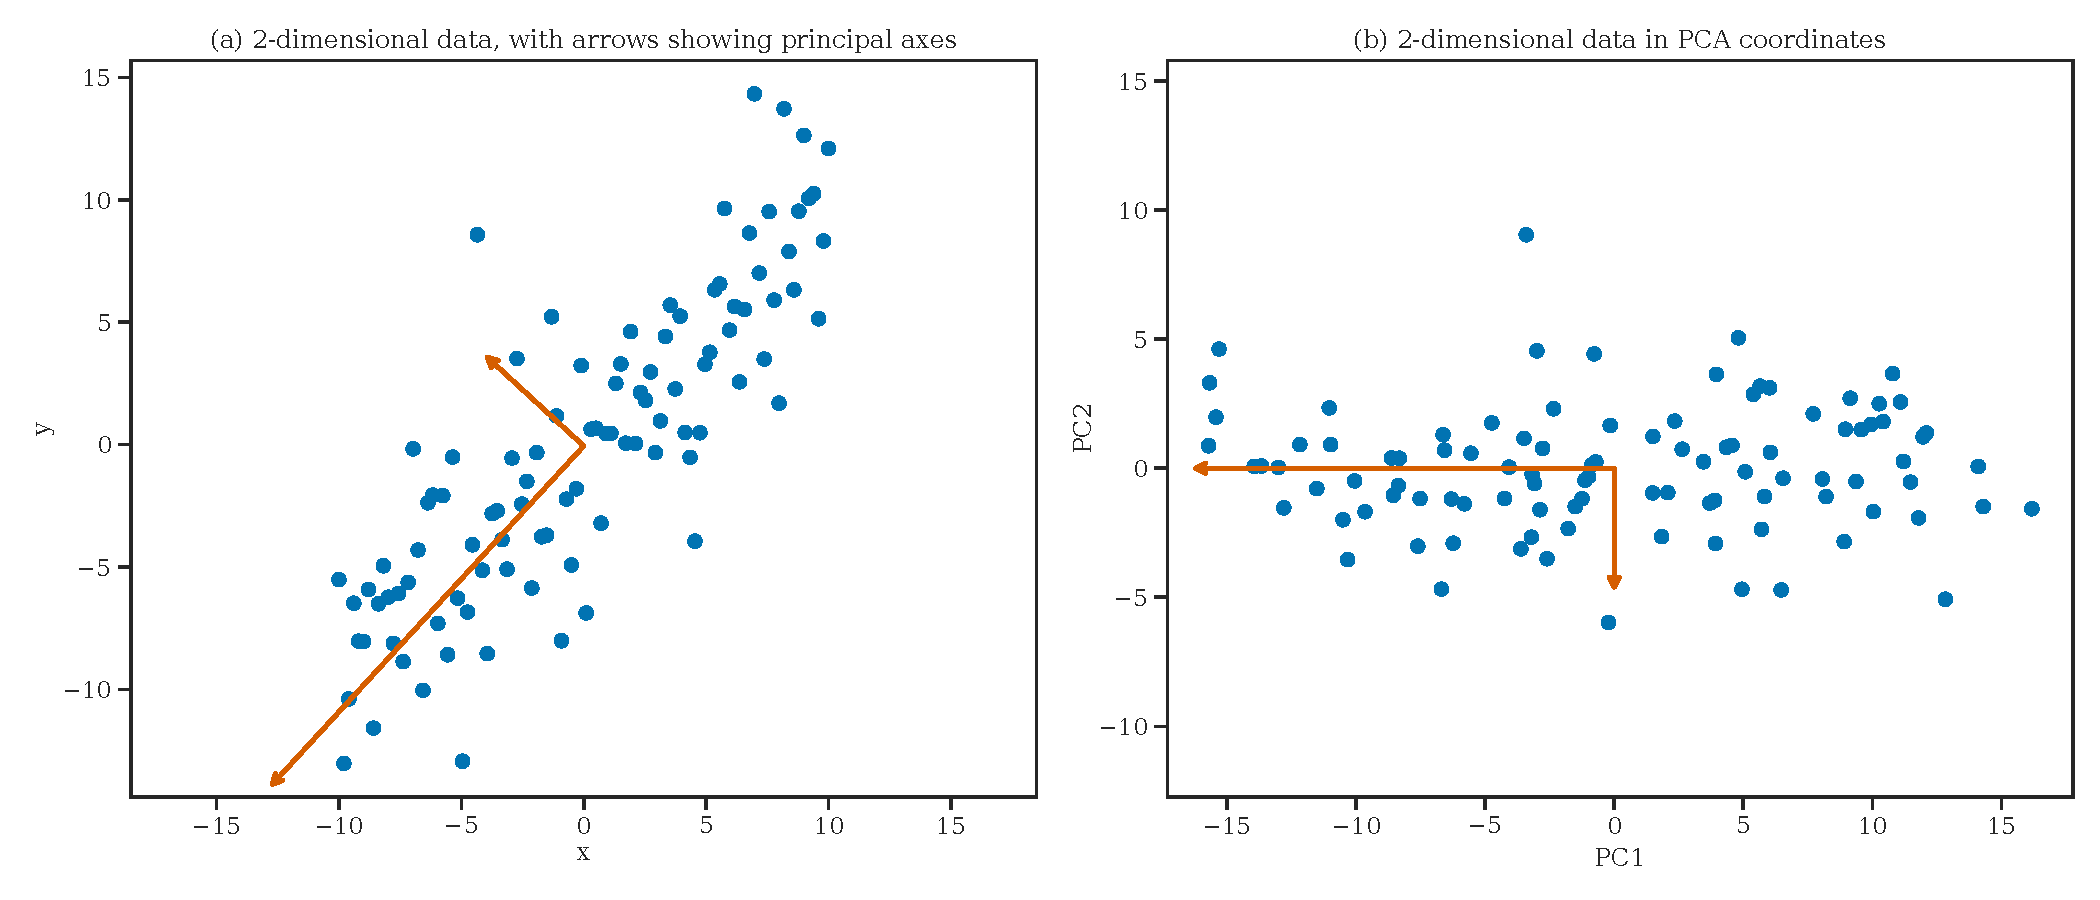
\includegraphics[width=\textwidth]{thesis/figures/pca-2d-example.pdf}
    \caption{PCA applied to 2-dimensional data, showing the principal axes by the arrows.}
    \label{fig:pca-2d-example}
\end{figure}

\subsubsection{Uniform Manifold Approximation and Projection}
\label{sec:umap}
\textit{Uniform Manifold Approximation and Projection} (UMAP) is a dimensionality reduction algorithm which, among other things, uses ideas from topological data analysis \cite{2018arXivUMAP}. In particular, UMAP uses a fuzzy version of simplicial complexes (see \cref{sec:simplicial-complex}) to create a graph representing the topological structure of the data in a higher dimension. To explain how UMAP works, we use the example from the "How UMAP Works" documentation page \cite{how-umap-works-2018}.

Imagine that we have some data from a noisy sine, $X = \enclc{x_1, x_2, \ldots, x_n} \in \R^{n \times d}$, as we see in \cref{fig:how_umap_works_raw_data}.
\begin{figure}[H]
    \centering
    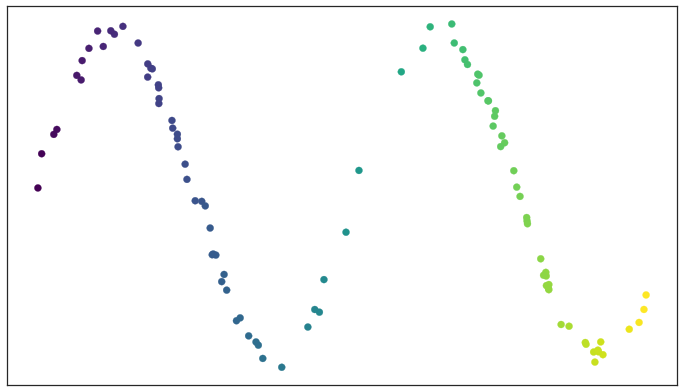
\includegraphics[width=0.8\textwidth]{thesis/figures/how_umap_works_raw_data.png}
    \caption{A noisy sine wave. The figure is from \cite{how-umap-works-2018}.}
    \label{fig:how_umap_works_raw_data}
\end{figure}

We would like to capture the topological structure of $X$, and we do so by creating a simplicial complex built on $X$, as we see in \cref{fig:how_umap_works_basic_graph}.
\begin{figure}[H]
    \centering
    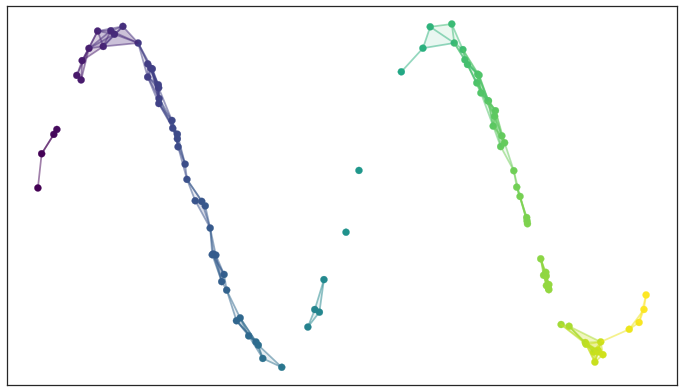
\includegraphics[width=0.8\textwidth]{thesis/figures/how_umap_works_basic_graph.png}
    \caption{A simplicial complex built on a noisy sine wave. The figure is from \cite{how-umap-works-2018}.}
    \label{fig:how_umap_works_basic_graph}
\end{figure}
We would like to capture the topological structure of all data points in $X$ and want a graph connecting all points. By using simplicial complexes, however, we see in \cref{fig:how_umap_works_basic_graph} that problems can occur, namely that not all data points have edges between them, which again disconnects the simplicial complex. This particular problem can occur when we have a too-small $\epsilon$ radius around each data point. In real-world data, the data points are typically not laying on a uniform distribution. Moreover, selecting a perfect $\epsilon$ to create a suitable simplicial complex is hard. The authors of UMAP overcome these problems by creating fuzzy open sets around each data point to create local connectivity in the graph, as we see in \cref{fig:how_umap_works_umap_open_cover}.
\begin{figure}[H]
    \centering
    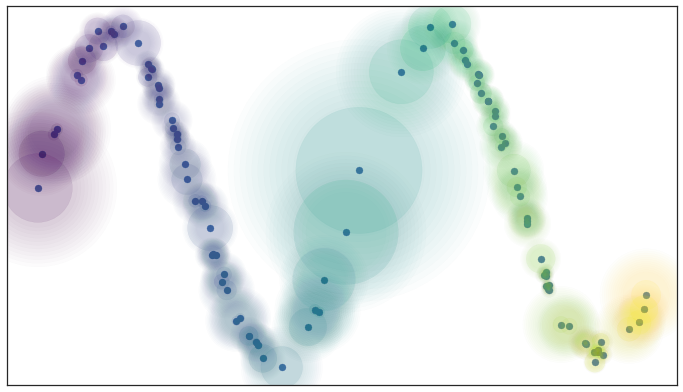
\includegraphics[width=0.8\textwidth]{thesis/figures/how_umap_works_umap_open_cover.png}
    \caption{Fuzzy open sets around each data point of a noisy sine wave to create local connectivity. The figure is from \cite{how-umap-works-2018}.}
    \label{fig:how_umap_works_umap_open_cover}
\end{figure}
To create the fuzzy open sets, we compute the distance to the nearest neighbour of each data point and the level of \textit{fuzziness} decreases in terms of the distance beyond it, starting from 1 decreasing to 0. If a data point has a fuzziness level greater than zero, then we create an edge between the two data points, with weight equal to the fuzziness level. Furthermore, we interpret the fuzziness level as the probability of the edge existing. We illustrate the connected graph in \cref{fig:how_umap_works_raw_graph}.

\begin{figure}[H]
    \centering
    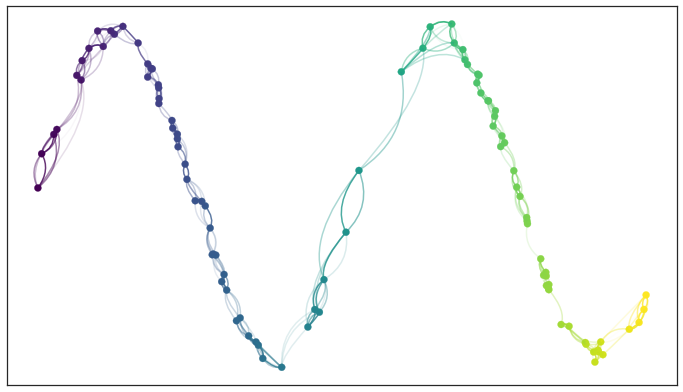
\includegraphics[width=0.8\textwidth]{thesis/figures/how_umap_works_raw_graph.png}
    \caption{A connected graph where nodes are data points and the edges between them have the fuzziness levels as weights. The figure is from \cite{how-umap-works-2018}.}
    \label{fig:how_umap_works_raw_graph}
\end{figure}
To finalize the connected graph from \cref{fig:how_umap_works_raw_graph}, we convert the edges between any two data points into a single edge. We do this because we want the distance between two data points $a$ and $b$ to be the same; currently, it depends locally on the distance to the nearest neighbour, as the fuzziness level decreases beyond it. To merge the edges between any two data points $a$ and $b$, we compute the combined weight by taking the union between them $w(a) + w(b) - w(a)w(b)$. We use the newly combined weight as the weight of the single edge between $a$ and $b$. If we apply this process, unioning edges together, we end up with a fuzzy simplicial complex. We show an example of a fuzzy simplicial complex in \cref{fig:how_umap_works_umap_graph}.
\begin{figure}[H]
    \centering
    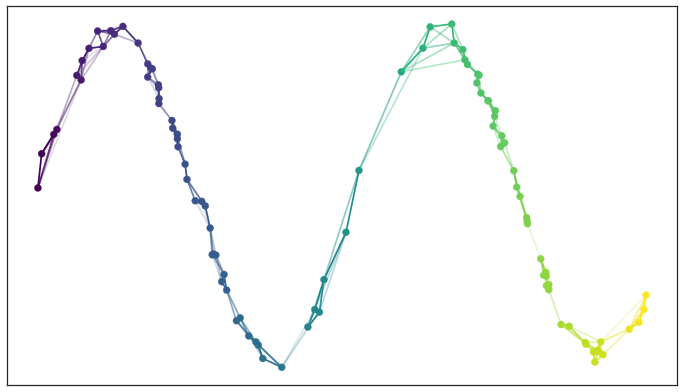
\includegraphics[width=0.8\textwidth]{thesis/figures/how_umap_works_umap_graph.png}
    \caption{A fuzzy simplicial complex of some sine wave data. The figure is from \cite{how-umap-works-2018}.}
    \label{fig:how_umap_works_umap_graph}
\end{figure}
Now, using the fuzzy simplicial complex of \cref{fig:how_umap_works_umap_graph}, we have a topological representation of $X$, capturing the topology of the manifold. We denote the set of all possible 1-simplices (i.e. edges) as $E$. To compute the weight of a 1-simplex (i.e. edge) $e$, we use $w_h(e)$ in the high dimensional case. To get a good low dimensional representation of the high dimensional fuzzy simplicial complex, we initialize a low dimensional fuzzy simplicial complex. We denote the weights of the low dimensional fuzzy simplicial complex as $w_l(e)$ for edge $e$. To determine the weights $w_l(e)$, we employ an iterative process where we optimize a loss function $L$ in a gradient descent fashion. Since we interpret the weights of the 1-simplices of $E$ as probabilities of the edge existing (i.e. Bernoulli variables), the authors of UMAP uses cross-entropy (see \cref{eqn:binary-cross-entropy}) as the loss function. More formally, we define the loss function $L$ as
\begin{align}
    L = \sumlim{e \in E}{} \undertext{w_h(e) \log \enclp{\frac{w_h(e)}{w_l(e)}}}{Attractive force} + \undertext{(1 - w_h(e)) \log \enclp{\frac{1 - w_h(e)}{1 - w_l(e)}}}{Repulsive force}.
    \label{eqn:umap-loss-function}
\end{align}

In the first term of \cref{eqn:umap-loss-function}, we have an attractive force between the data points which $e$ spans, pulling them together; when $w_l(e)$ is large, the distance (i.e. weight) between any two data points becomes small. In the second term of \cref{eqn:umap-loss-function}, there is an opposite, repulsive force between the data points which $e$ spans, repelling them apart; when $w_h(e)$ is small (i.e. distance in high dimensional space), $w_l(e)$ becomes small since we want to minimize the term. The process of pulling and repelling the weights makes the low dimensional representation of the data settle into a balanced state, such that it represents the high dimensional topological structure of the original data in a fairly accurate way. In practice, the UMAP algorithm uses several different tricks to optimize it, but we leave out the technical details here. We kindly refer the reader to \cite{2018arXivUMAP} for more details. Finally, we show an example where we compute a 2-dimensional UMAP embedding of the Iris data set \cite{Anderson1936,Fisher1936} in \cref{fig:umap-2d-example}. In \cref{fig:umap-2d-example}, we see that UMAP can separate the classes in the Iris data set quite nicely, particularly for the \textit{setosa} class.
\begin{figure}[H]
    \centering
    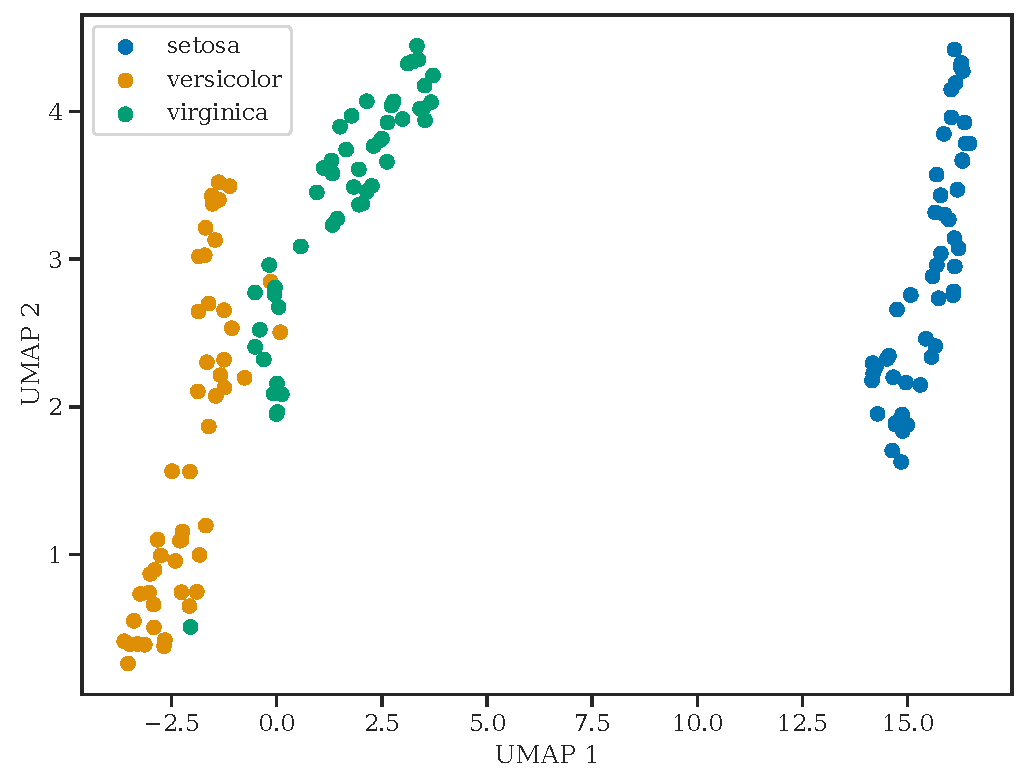
\includegraphics[width=0.8\textwidth]{thesis/figures/umap-2d-example.pdf}
    \caption{2-dimensional UMAP embedding of the Iris data set \cite{Anderson1936,Fisher1936}.}
    \label{fig:umap-2d-example}
\end{figure}

\subsection{Artificial neural networks}
\label{sec:artificial-neural-networks}
In this subsection we explain \textit{artificial neural networks} (ANN). In particular, we focus on \textit{multilayered neural networks} (MLNN). We base this subsection on \cite[Chapter 1]{Aggarwal18} and \cite{rong2016word2vec}. Furthermore, we will use the notion of artificial neural networks when we explain the word2vec model in \cref{sec:word2vec-as-an-ann}.

An \textit{artificial neuron} (or \textit{unit}) is a function which receives one or more inputs and a \textit{bias}, and then sums them to produce an output. We illustrate an example of an artificial neuron in \cref{fig:artificial_neuron}, where $\left\{ x_1, \ldots, x_K \right\}$ are the input values, $b$ is the bias, $\left\{ w_1, \ldots, w_K \right\}$ are the weights and $y$ is a scalar output. We denote $f$ as the \textit{activation function}.
\begin{figure}[H]
    \centering
    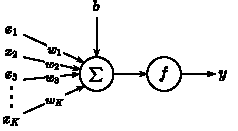
\includegraphics[width=0.5\textwidth]{thesis/figures/artificial-neuron_cropped.pdf}
    \caption{An artificial neuron that takes in a $K$-dimensional input $x$ and bias $b$ to produce some output $y$.}
    \label{fig:artificial_neuron}
\end{figure}

We produce the output of a single unit by applying an activation function $f$ to the input $u$. More formally, we define the output of a single unit as
\begin{align}
    y = f(u),
\end{align}
where $u$ is the input of the neuron. We define $u$ as
\begin{align}
    u = b + \sumlim{i=1}{K} w_i x_i,
\end{align}
which is the weighted sum of the input values $\left\{ x_1, \ldots, x_K \right\}$ plus the bias term, with $\left\{ w_1, \ldots, w_K \right\}$ as weights.

The bias term acts as an intercept value to make the model more general and is usually set to +1. For some models (e.g. word2vec, which we introduce as an ANN in \cref{sec:word2vec-as-an-ann}), we exclude the bias term for the units in the neural network, i.e. we leave $b$ to be zero.

The choice of activation function $f$ is typically a non-linear function. Artificial neural networks use different activation functions such as ReLU, sigmoid or tanh to learn non-linear relationships in the data. We come back to the concept of activation functions in \cref{sec:ann-activation-functions}.

\newcommand{\layer}[2]{\left\{ {#1}_{#2} \right\}}

A \textit{layer} $\layer{z}{j} = \left\{ z_1, z_2, \ldots, z_K \right\}$ of an artificial neural network is a collection of artificial neurons (unit). We define the layer $\layer{z}{j}$ using an $N \times K$-dimensional weight matrix $W$, a $N$-dimensional bias vector $b$ and an activation function $f$. More formally, we define a layer $\layer{z}{j}$ as
\begin{align}
    \layer{z}{j} = f \left( W \cdot x + b \right),
    \label{eqn:artificial_layer}
\end{align}
where $x$ is a $K$-dimensional input vector. In the following sub-subsections, we explain the different types of layers in the ANN, namely the input, hidden and output layers.

\subsubsection{Input layer}
\label{sec:ann-input-layer}
The first layer in the ANN is the \textit{input layer} $\layer{x}{k} = \left\{ x_1, x_2, \ldots, x_K \right\}$. It is responsible for taking in input and passing it to the proceeding layer in the network. We illustrate the input layer in \cref{fig:input_layer_ann}, where we see that each input value $x_i$ gets its own node.
\begin{figure}[H]
    \centering
    
\includegraphics[height=5cm]{thesis/figures/artificial-neural-network-input-layer_cropped.pdf}
    \caption{Input layer in the ANN for a $K$-dimensional vector $x$.}
    \label{fig:input_layer_ann}
\end{figure}
Following, we define the input layer more formally using \cref{eqn:artificial_layer} in \cref{eqn:input_layer_ann}. We see that the input layer does not perform any changes to the incoming data and acts as a way for feeding data into the neural network. More formally, we define the input layer $\layer{x}{k}$ as
\begin{align}
    \label{eqn:input_layer_ann}
    \layer{x}{k}
    &= f_{\layer{x}{k}}(W_{\layer{x}{k}} \cdot x) \\
    &= id(I_K \cdot x) \notag \\ 
    &= I_K \cdot x \notag \\
    &= x, \notag
\end{align}
where the weight matrix $W_{\layer{x}{k}}$ is the identity matrix $I_K$, we have no bias (i.e. bias equal to zero vector) and the activation function $f_{\layer{x}{k}}$ is the identity function $id(x)=x$. In the following sub-subsection, we look at the next layer in the neural network, namely the hidden layer.

\subsubsection{Hidden layer}
\label{sec:ann-hidden-layer}
The \textit{hidden layer} is the second layer in the ANN $\layer{h}{i} = \left\{ h_1, h_2, \ldots, h_N \right\}$, and we most commonly connect it to the input layer. We note that we can, however, have multiple hidden layers in the ANN (making the neural network \textit{deeper}), by connecting them to each other. For illustration purposes, we assume that we only have one hidden layer in our neural network. We illustrate an example of a hidden layer in \cref{fig:hidden_layer_ann}, where we observe that we connect every unit in the input layer to the units in the hidden layer. We illustrate the connections by the lines. This is what we call \textit{fully connected layers}, meaning that we connect every unit to each other.

\begin{figure}[H]
    \centering
    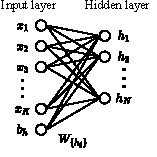
\includegraphics[height=6cm]{thesis/figures/artificial-neural-network-input-hidden-layer_cropped.pdf}
    \caption{Input to hidden layer in the ANN for a $K$-dimensional vector $x$, $N\times K$ dimensional weight matrix $\left\{ W_{h_i} \right\}$ and a $N$-dimensional hidden layer $h$.}
    \label{fig:hidden_layer_ann}
\end{figure}
We formalize the description of the hidden layer by defining it as
\begin{align}
    \label{eqn:hidden-layer-ann}
    \layer{h}{i} &= f_{\layer{h}{i}}(W_{\layer{h}{i}} \cdot \layer{x}{k} + b_h),
\end{align}
where $f_{\layer{h}{i}}$ is a user-specified activation function, $W_{\layer{h}{i}}$ is an $N \times K$-dimensional weight matrix and $b_h$ is an $N$-dimensional bias vector. The hidden layer tries to learn a \textit{latent} (i.e hidden) representation of the input data $x$. We explain how the neural network learns the latent representation when introducing optimizers in \cref{sec:ann-optimizers}. Assuming that we have some $N$-dimensional latent representation of the data, we would like to connect it to the final layer in the neural network, the output layer, which we explain next.

\subsubsection{Output layer}
\label{sec:ann-output-layer}
The last layer in the ANN is the \textit{output layer} $\layer{y}{j} = \left\{ y_1, y_2, \ldots, y_M \right\}$, which we connect to the last hidden layer of the network. Similar to the hidden layer, we connect each unit in the last hidden layer to each unit in the output layer. We illustrate an example of this in \cref{fig:mlnn-one-hidden}, where we see a complete, multilayered neural network (MLNN).
\begin{figure}[H]
    \centering
    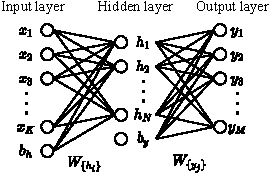
\includegraphics[width=0.6\textwidth]{thesis/figures/artificial-neural-network_cropped.pdf}
    \caption{Multilayered neural network with one input, hidden and output layer.}
    \label{fig:mlnn-one-hidden}
\end{figure}

Following, we define the output layer $\layer{y}{j}$ using a $M \times N$ weight matrix $W_{\layer{y}{j}}$, an $M$-dimensional bias vector $b_y$ and an activation function $f_{\layer{y}{j}}$. More formally, we define the output layer $\layer{y}{j}$ as
\begin{align}
    \label{eqn:output-layer-ann}
    \layer{y}{j} &= f_{\layer{y}{j}}(W_{\layer{y}{j}} \cdot \layer{h}{i} + b_y).
\end{align}

We have now covered the different layers in an MLNN, but have yet to cover the different choices of activation function $f$ in the neural network and how the MLNN learns. In the following sub-subsections, we look at choices of activation and loss functions, as well as optimizers for learning in the network.

\subsubsection{Activation functions}
\label{sec:ann-activation-functions}
The input data we use to feed into an ANN can contain complex patterns and have non-linear relationships. To learn such patterns and relationships, we apply an activation function to each layer before the result is sent to the proceeding layer. There are several choices of activation functions and following, we explain some of the most common ones.

The simplest type of activation is the identity function, which we define as
\begin{align}
    \label{eqn:identity-function}
    f(x) = x.
\end{align}
We commonly use the identity function when we want to pass on the values from one layer to another without modifying the value itself, as we use in the input layer from \cref{sec:ann-input-layer}. Other choices of activation functions include \textit{sigmoid}, \textit{tanh}, \textit{Rectified Linear Unit} (ReLU) and \textit{softmax}. We visualize activation functions in \cref{fig:activation-functions} and define them formally below as
\begin{align}
    \label{eqn:sigmoid-function}
    f(x) &= \frac{1}{1 + \exp{ \left( -x \right) }} \thickspace \text{(sigmoid function)}, \\
    \label{eqn:tanh-function}
    f(x) &= \frac{\exp{ \left( 2x \right) } - 1}{\exp{ \left( 2x \right) } + 1} \thickspace \text{(tanh function)}, \\
    \label{eqn:relu-function}
    f(x) &= \max{\left\{ x, 0 \right\}} \thickspace \text{(ReLU function)}, \intertext{and}
    \label{eqn:softmax-function}
    f(x_i) &= \frac{\exp \left( x_i \right)}{\sumlim{j=1}{K} \exp \left( x_j \right)} \thickspace \text{, $i \in \left\{ 1, \ldots, K \right\}$ (softmax function)},
\end{align}
where $K$ is the number of output values for the softmax layer.

\begin{figure}[H]
    \centering
    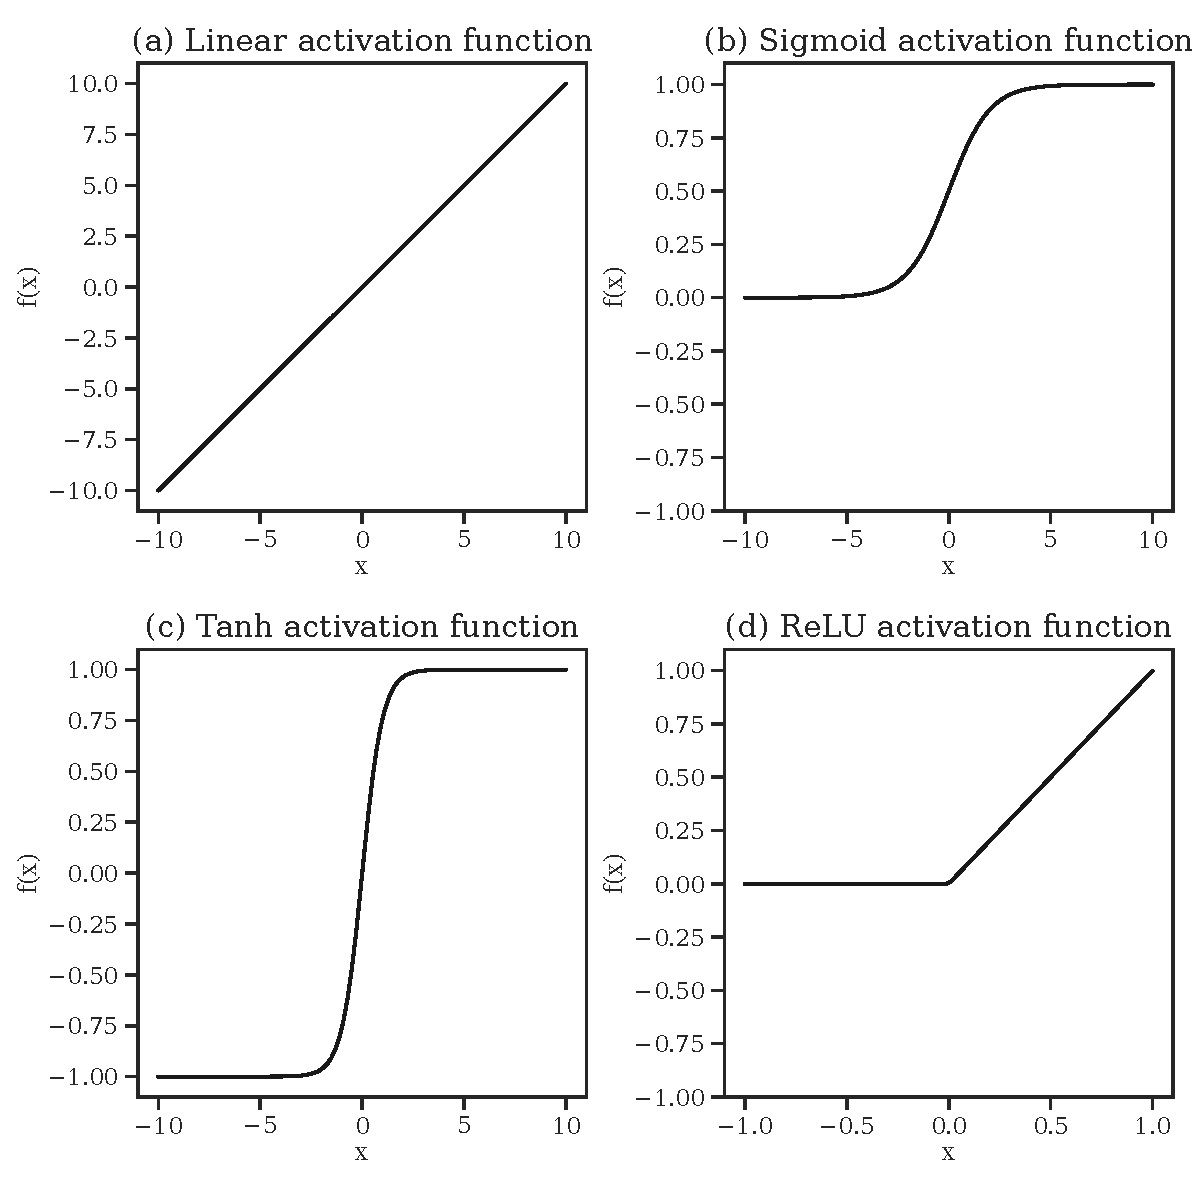
\includegraphics[width=0.8\textwidth]{thesis/figures/common-activation-functions.pdf}
    \caption{Four plots of various activation functions showing how they respond to different values of $x$.}
    \label{fig:activation-functions}
\end{figure}

The sigmoid and tanh activation functions were typically used in the early development of neural networks. The sigmoid activation function maps a value to a value in $(0, 1)$ and is particularly useful since it creates a probabilistic output. The tanh activation function has a similar shape to the sigmoid activation function and maps values to values in $[-1, 1]$. We show the relationship between the tanh and sigmoid activation functions as
\begin{align}
    \label{eqn:tanh-sigmoid-relation}
    \text{tanh}(x) = 2 \cdot \text{sigmoid}(2x) - 1,
\end{align}
where we see that the tanh activation function is a rescaled version of the sigmoid activation function.

In more recent years, the ReLU activation function has become more popular, partly due to its computational simplicity. Both the sigmoid and tanh activation function suffers from \textit{vanishing gradients} (i.e. gradients become zero, leading to very little learning) and we typically use ReLU as a substitute to overcome this problem. This does not mean, however, that we can use the ReLU activation function without problems, as it can "die out" since it is non-differentiable at 0.

Up until now, we have only explained activation functions in the context of a single output value. To perform classification with $K$ outputs, we typically use the softmax activation function, which we define in \cref{eqn:softmax-function}. We interpret the output of the softmax activation function as the probabilities of the $K$ outputs. Next, we look at loss functions in neural networks.

\subsubsection{Loss functions}
\label{sec:ann-loss-functions}
By connecting the different layers in an ANN, we have seen how we use some input data, send it through some hidden layer, and finally, get the predicted output values from the output layer. We denote the predicted output values as $\hat{y}$ and assume that we have the true output values as well, which we denote $y$. The \textit{loss function} measures how much the predicted values $\hat{y}$ deviate from the true values $y$, and as such, the goal is to minimize this value. The output layer can have one or many outputs, and depending on the configuration of the network, the loss function changes as well. We separate the output types of an ANN into two categories, namely the \textit{regression} and \textit{classification} outputs.

In a regression type output, we usually predict some real-value quantity, such as height, weight or distance. For such problems, it is common to use the \textit{mean squared error} (MSE) as the loss function. We calculate the MSE as the mean of the squared differences between the predicted and true values. More formally, we define MSE as
\begin{align}
    \label{eqn:mean-squared-error}
    \text{MSE}(\hat{y}, y) = \frac{1}{N} \sumlim{i=1}{N} {\left( y_i - \hat{y_i} \right)}^2,
\end{align}
where $N$ is the length of $y$ and $\hat{y}$.

For classification type outputs, we want to classify whether or not some input data belongs to two (binary, e.g. on or off, blue or red) or more classes (categorical, e.g. different types of animals). In a binary classification type output, we use the sigmoid activation function in conjunction with the \textit{binary cross-entropy} (BCE) loss function. We define the binary cross-entropy loss function as
\begin{align}
    \label{eqn:binary-cross-entropy}
    \text{BCE}(\hat{y}, y) = -\left( y \cdot \log{\left( \hat{y} \right)} + (1 - y) \cdot \log{\left( 1 - \hat{y} \right)} \right).
\end{align}
As opposed to the binary cross-entropy function, we use the \textit{categorical cross-entropy} (CCE) function to compute the loss for multi-class classification output. We commonly use the softmax activation function in the output layer to create a multi-class probability distribution. Furthermore, we define the CCE loss function as
\begin{align}
    \label{eqn:categorical-cross-entropy}
    \text{CCE}(\hat{y}, y) = -\sumlim{c=1}{C} y_c \cdot \log{\left( \hat{y_c} \right)},
\end{align}
where $C$ is the number of classes in the multi-class classification output. From \cref{eqn:categorical-cross-entropy}, we observe that CCE is simply a generalization of the BCE loss function for multiple classes.

\subsubsection{Optimizers}
\label{sec:ann-optimizers}
In this sub-subsection, we explain how an ANN can effectively make predictions from input data by learning its internal weights. In particular, we explain the gradient descent algorithm and how ANNs exploit it to perform efficient training of its internal parameters.

So far, we have discussed what we call the \textit{forward pass} (or phase). A forward pass is simply the journey of the input data to the output layers where we in each step compute the output values at each layer and local derivatives using the current set of weights. Once we are at the output layer, the forward pass is complete and the \textit{backward pass} commences. Recall that the objective of the neural network is to minimize the loss function. To do so, we compute the derivative of the loss function with respect to the weights in the input layer, using the chain rule from calculus. The derivative of the loss function tells the neural network which direction it should move each weight in to minimize the loss (i.e. in the negative direction of the derivative). To give an example of forward and backward passes in an ANN, consider the example in \cref{fig:neural-network-example-backprop}.
\begin{figure}[H]
    \centering
    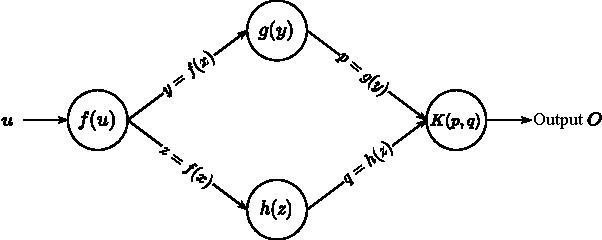
\includegraphics[width=0.7\textwidth]{thesis/figures/artificial-neural-network-backprop-example_cropped.pdf}
    \caption{A neural network with one input node, one hidden layer with two nodes and one output layer.}
    \label{fig:neural-network-example-backprop}
\end{figure}

In \cref{fig:neural-network-example-backprop}, we have a network with one input node (neuron), a hidden layer with two nodes and a single output layer with one node. We denote the input to the network as $u$, which is the product of the input data and the weights in the input layer. For the activation functions of the network, we denote them as $f$, $g$ and $h$. Moreover, we denote the results of the activation functions as $y$, $z$, $p$, $q$, and the function $K$ combines the result of $p$ and $q$ resulting in the output value $O$. We assume that we apply the weights of the hidden layer to the previous layer's output values during $g$ and $h$ and that we apply the weights of the output layer at $K$. The forward pass in this network is straightforward: We start the input node, pass the data on to $g$ and $h$ and combine the results in the output layer. Now, for the backwards pass, we first compute the loss at the output node using a loss function $L$. Furthermore, we compute the derivative of $L$ with respect to the input $u$. More formally, we compute
\begin{align}
    \parder{L}{u}
    &= \parder{L}{O} \cdot \parder{O}{u} \label{eqn:derivative-of-l-wrt-u} \\
    &= \parder{L}{O} \cdot \left[
    \parder{O}{p} \cdot \parder{p}{u} +
    \parder{O}{q} \cdot \parder{q}{u}
    \right] \text{(chain rule)} \notag \\
    &= \parder{L}{O} \cdot \left[
    \parder{O}{p} \cdot \parder{p}{y} \cdot \parder{y}{u} + 
    \parder{O}{q} \cdot \parder{q}{z} \cdot \parder{z}{u}
    \right] \text{(chain rule)} \notag \\
    &= \parder{L}{O} \cdot \left[
    \undertext{\parder{K(p, q)}{p} \cdot g'(y) \cdot f'(u)}{Path on top} + 
    \undertext{\parder{K(p, q)}{q} \cdot h'(z) \cdot f'(u)}{Path on bottom} \notag
    \right].
\end{align}
From \cref{eqn:derivative-of-l-wrt-u}, we see how to calculate the derivatives for a relatively small neural network. There exists, effective and more general frameworks to derive the derivative of the loss with respect to the input values, but we leave those details out and kindly refer the reader to \cite[Chapter 1.3]{Aggarwal18} for more details.

We have now gone over the forward and backward passes, which are the first two steps of the so-called backpropagation algorithm. The remaining step of the algorithm is to use the computed derivatives to update the weights of the ANN. To do this, we use the \textit{gradient descent} (GD) algorithm. The main idea of gradient descent is to update the weights iteratively by moving them in the opposite direction of the gradient (i.e. the steepest descent) of the loss with respect to the weights. By doing so, it leads to better-fitting weights for the input-output data. In standard gradient descent, we perform its steps by
\begin{align}
    W \Leftarrow W - \alpha \cdot \parder{L}{W},
\end{align}
where $W = \left( w_1, w_2, \ldots, w_d \right)$ is the matrix consisting of the $d$ weights of an ANN. The learning rate $\alpha$ is a hyperparameter and determines how much learning we want to do in each step. The learning rate is usually set to a relatively low value, in the order of $10^{-2}$ to $10^{-5}$. We illustrate the effect of the gradient descent algorithm with a small example in \cref{fig:gradient-descent-example}, where we compute gradient descent for the paraboloid $f(x, y) = (x - 2)^2 + (y - 4)^2$. We set the starting point to be (-5, -10), the learning rate $\alpha$ to 0.05 and use 100 iterations. In \cref{fig:gradient-descent-example}, we see that the gradient descent algorithms finds the minimum of $f(x, y)$ relatively fast.
\begin{figure}[H]
    \centering
    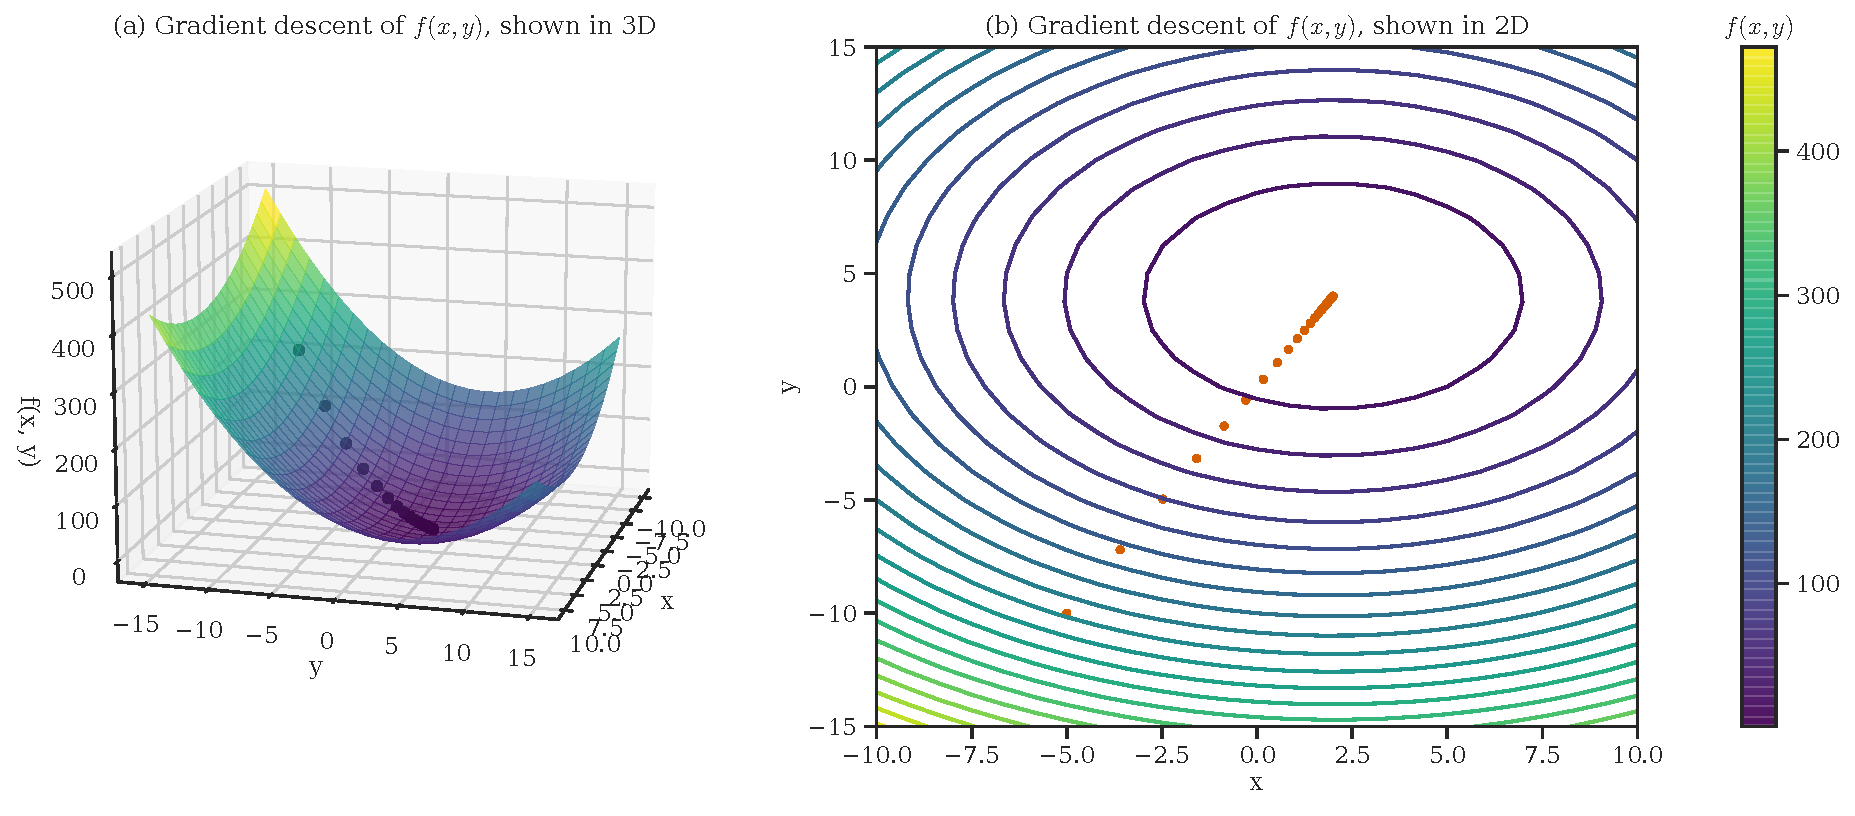
\includegraphics[width=\textwidth]{gradient-descent-example}
    \caption{Gradient descent of the function $f(x, y) = (x - 2)^2 + (y - 4)^2$. We start at point (-5, -10), use a learning rate $\alpha$ of 0.05 and compute for 100 iterations.}
    \label{fig:gradient-descent-example}
\end{figure}

Even though gradient descent works great for small applications, once we scale the number of parameters (weights) in the ANN to the more extremes (e.g. in the order of millions), it becomes impractical to compute for the entire training data at once. Furthermore, we observe that a loss function $L$ usually can be written as a sum of the loss of the individual training data points, where $L_i$ is the loss for training data point $i$. Thus, we define the individual loss $L_i$ as
\begin{align}
    \label{eqn:loss-function-sum-individual}
    L = \sumlim{i=1}{n} L_i.
\end{align}
Using the observation that we are able to write the loss function as the sum in \cref{eqn:loss-function-sum-individual}, we introduce the \textit{stochastic gradient descent} (SGD) method. Instead of performing gradient descent on the whole input data, SGD performs gradient descent for each input data separately. More formally, SGD performs its steps by
\begin{align}
    \label{eqn:sgd}
    W \Leftarrow W - \alpha \cdot \parder{L_i}{W},
\end{align}
where $n$ is the number of input data points and $L_i$ represents the loss of the $i$th input. We call SGD stochastic because a random sample of the training data is chosen for each iteration. An advantage that SGD has over GD, is that it runs a lot faster, at the expense of greater loss. Thankfully, there exists a variant of SGD which seeks to find a balance between speed and loss, namely the \textit{mini-batch stochastic gradient descent} (mini-batch SGD) method. In mini-batch SGD, we use a batch $B=\enclc{j_1, \ldots, j_m}$ of input training data indices when computing the weight updating. In other words, mini-batch SGD performs its steps by
\begin{align}
    \label{eqn:mbsgd}
    W \Leftarrow W - \alpha \cdot \sumlim{j \in B}{} \parder{L_j}{W}.
\end{align}
Mini-batch SGD often finds the best trade-off between stability, speed and memory requirements. However, we note that the memory requirement increases with the use of mini-batches. This is because we have to store bigger matrices in memory during training. We typically choose batch sizes that are a power of 2 (e.g. 32, 64, 128 or 256), as most modern hardware architectures optimize for such values.

In addition to the different variants of gradient descent, there exist a bunch of other variants which can solve issues such as getting stuck in local minima or speeding up the training process. We leave out the technical details of all these strategies here, but kindly refer the reader to \cite[Chapter 3.5]{Aggarwal18} for more details.

\subsection{Intrinsic dimension estimation}
\label{sec:intrinsic-dimension-estimation}
In machine learning, the \textit{manifold hypothesis} states that, in general, real-life high-dimensional data tends to live on a low-dimensional submanifold embedded within the high-dimensional space \cite[p. 16]{bengio2014representation}. To understand more about the underlying structure of the data we are working with, we can estimate the dimension of the low-dimensional submanifold. We call the process of estimating the dimension of the low-dimensional submanifold \textit{intrinsic dimension (ID) estimation}. More generally, a $D$-dimensional data set $X \in \R^D$ is said to have an ID equal to $d$ if $X$ lies entirely within a $d$-dimensional subspace of $\R^D$ \cite{lee2015intrinsic}. We separate between \textit{global} and \textit{local} ID estimation methods, where global methods estimate the ID for the entire data set, and local methods estimate ID for each data point in the data set. We note, however, that it is fully possible and common in the literature to approximate local ID estimates by computing global ID estimates of a $k$-nearest neighbourhood around each data point $x \in X$. In the following sub-subsections, we introduce five methods for estimating the ID. We leave out the technical details of the ID estimation methods, as they are not the focus of this thesis. Instead, we give an overall explanation for each of the methods, and kindly refer the reader to the source of each method for more details. For each of the methods we describe below, we assume that we have some data set $X \in \R^{N \times D}$ consisting of $N$ samples, where each sample is a $D$-dimensional vector. We base this subsection on \cite{lee2015intrinsic} if we do not state otherwise. Following, our interest is mainly in local ID estimation methods for this thesis, as we will use them for the analysis of word embeddings (\cref{sec:word-embeddings}) in \cref{sec:analysis-of-embeddings-intrinsic-dimension-estimation} and for polysemous word prediction in \cref{sec:analysis-of-embeddings-supervised-polysemy-prediction}.

\subsubsection{LPCA}
\label{sec:id-estimation-lpca}
One of the first and most simple kinds of ID estimation algorithm bases itself on the PCA algorithm (see \cref{sec:pca}). In particular, the ID estimation algorithm uses information from the eigenvalue decomposition of PCA to estimate the intrinsic dimension. We refer to this ID estimation algorithm as the \textit{local PCA} (LPCA) method, which was first introduced in \cite{Fukunaga1971}. We refer to \cite{Fukunaga1971} when explaining the LPCA method. The LPCA method works as follows. First, we reducing the dimensionality of the original data set $X$ from $D$ dimensions to $\hat{d}$ dimensions, by applying PCA and making sure that most of the variance in the $\hat{d}$ dimensions are kept. To select $\hat{d}$, LPCA counts the number of eigenvalues that are greater than a portion $\alpha$ of the largest eigenvalue, from PCAs eigenvalue decomposition. A typical value for $\alpha$ is 0.1, meaning that $\hat{d}$ is set to the number of eigenvalues that are greater than 90\% of the largest eigenvalue. The value $\hat{d}$ is then the estimated ID. The LPCA algorithm for estimating ID is a local estimator, meaning that estimates the ID for every data point $x \in X$. We typically implement LPCA using $k$-nearest neighbour, meaning that for every data point $x \in X$, we compute PCA of the $k$-nearest neighbourhood around $x$ to estimate its ID.

\subsubsection{KNN}
\label{sec:id-estimation-knn}
A popular approach to estimate the ID is to use $k$-nearest neighbour ($k$-NN) graphs. In this sub-subsection, we explain the \textit{$k$-NN algorithm} for ID estimation, as explained by \cite[p. 651]{Carter2010}. The $k$-NN algorithm uses the notion of the total edge length of the $k$-NN graph built on the data $X$, to estimate the ID $\hat{d}$. Let $D(x_i, x_j)$ denote the distance between two data points $x_i, x_j \in X$, and let $\mathcal{N}_{k, i}$ denote the set of the $k$-nearest neighbours of data point $x_i$. Then, we define the total edge length of the $k$-NN graph as
\begin{align}
    L_{\gamma, k}(X) = \sumlim{i=1}{n} \sumlim{y \in \mathcal{N}_{k, i}}{} D(x_i, x_j)^\gamma,
    \label{eqn:k-nn-id-estimation-l}
\end{align}
where $\gamma>0$ is a constant, weighting the distances between the data points in the $k$-NN graph. If we let $\gamma>1$, then we emphasize big distances between data points. The authors of \cite[p. 651]{Carter2010} then argue that, assuming the manifold hypothesis holds for the data $X$ (i.e. that the data $X$ can be fully described using a submanifold $X' \in \R^{N \times d}$), it is possible to estimate $\hat{d}$ by applying non-linear least squares to an approximation of the total edge length. The $k$-NN algorithm for estimating ID is a global estimator, meaning that estimates the ID of the whole data $X$. It is possible to make it local by applying the procedure we explained in the introduction to ID estimation in \cref{sec:intrinsic-dimension-estimation}.

\subsubsection{TWO-NN}
\label{sec:id-estimation-twonn}
Estimating the ID can be a hard task, especially if the underlying manifold of the data is twisted and curved. It is for this reason, the authors of \cite{Facco2017twonn} propose a two nearest neighbours estimator for ID estimation, which we refer to as the \textit{TWO-NN} method. TWO-NN uses the first and the second nearest neighbour of each data point in $X$ to estimate the ID. The authors of \cite{Facco2017twonn} show that by using the ratio of the distance to the second nearest neighbour to the first one to create a linear regression model which estimates the ID $\hat{d}$. Following, the authors claim that this minimality reduces the effect of complex manifolds, varying density and reduces the computational cost. The TWO-NN algorithm for estimating ID is a global estimator, meaning that estimates the ID of the whole data $X$. It is possible to make it local by applying the procedure we explained in the introduction to ID estimation in \cref{sec:intrinsic-dimension-estimation}.

\subsubsection{MLE}
\label{sec:id-estimation-mle}
Maximum likelihood estimation (MLE) is a method for estimating the parameters of a probability distribution, by either maximizing a likelihood function. \cite{Levina2004} propose a method that uses MLE to estimate the ID of data points $x \in X$. The idea is to estimate the ID locally, by assuming that the density $f(x)$ is constant for a small sphere $S_x(R)$ of radius $R$ around $x$. Then, they use a Poisson process to measure the rate of the counting process $N(t, x)$ which measures the number of points falling onto the sphere $S_x(R)$ at time $t$. Furthermore, they use MLE on the Poisson process to estimate the local ID $\hat{d}$ for point $x$. Note that in practice, it is common to use $k$-nearest neighbours instead of radius $R$ to find neighbours of $x$. An extension of the MLE method for estimating local ID was proposed by \cite{Haro2008}, which makes the ID estimator more robust to noise.

\subsubsection{TLE}
\label{sec:id-estimation-tle}
\textit{Tight Local Intrinsic Dimensionality Estimator} (TLE) \cite{Amsaleg2019} is a method for estimating the local ID of data points $x \in X$. The authors of TLE claim that the method works well in tight localities, i.e. within neighbourhoods of small size (e.g. using $k$-nearest neighbour). By using distances from $x$ to its $k$-nearest neighbours, TLE estimates the local ID $\hat{d}$. The authors of \cite{Amsaleg2019} claim that TLE can achieve more accurate ID estimates within small neighbourhoods around $x$ (i.e. for small values of $k$), which again can improve the quality of algorithms that depend on local ID estimates.

\subsection{Regression analysis}
\label{sec:regression-analysis}
\textit{Regression analysis} is a set of methods from statistics to estimate relationships between a \textit{dependent variable} and one or more \textit{independent variables}. To give an example, a dependent variable could be "income" and independent variables could be "education" and "experience". Regression analysis could help us to understand how income is affected by education, for instance. In this subsection, we look at three regression methods in particular: linear regression, lasso regression and logistic regression. We refer to \cites{James2013}{fox2015applied} \, when describing concepts from regression analysis. Furthermore, we will use the lasso and logistic regression methods for the prediction of polysemous words in \cref{sec:analysis-of-embeddings-supervised-polysemy-prediction}.

\subsubsection{Linear regression}
\label{sec:linear-regression}
\textit{Linear regression}, as the name suggests, attempts to find linear relationships between variables. The simplest form of linear regression is between a dependent variable $X$ and a single independent variable $Y$. First, we assume that there is an approximately linear relationship between $X$ and $Y$. Then, we model the linear relationship as
\begin{align}
    Y \approx \beta_0 + \beta_1 X,
\end{align}
where the approximate equals sign "$\approx$" means that we are \textit{regressing} $Y$ onto $X$. The two constants $\beta_0$ and $\beta_1$ are unknown and represents the \textit{intercept} and \textit{slope} in terms of the linear model. We refer these two constants as the \textit{model parameters}. Following, we use some training to compute estimates of the models parameters, $\hat{\beta_0}$ and $\hat{\beta_1}$. We use the \textit{hat} symbol, $\string^$\,, to denote some estimated or predicted value. To predict future values for $Y$, we use the estimated parameters $\hat{\beta_0}$ and $\hat{\beta_1}$ by computing
\begin{align}
    \hat{Y} = \hat{\beta_0} + \hat{\beta_1}X,
    \label{eqn:y-hat-simple}
\end{align}
where $\hat{Y}$ is the predicted value of $Y$. To estimate the model parameters $\hat{\beta_0}$ and $\hat{\beta_1}$, we must use some training data. Now, we let $X = (x_1, x_2, \ldots, x_n) \in \R^n$ and $Y = (y_1, y_2, \ldots, y_n) \in \R^n$ represent our data as two $n$-dimensional vectors. In machine learning terms, we are in a supervised setting, since we know the true labels $y$ before trying to predict them. After applying some linear algebra, we rewrite $\cref{eqn:y-hat-simple}$ for a single data point $i$ as
\begin{align}
    \hat{y_i} =
        \begin{bmatrix}
            1 & x_i
        \end{bmatrix}
        \begin{bmatrix}
            \hat{\beta}_0 \\
            \hat{\beta}_1 \\
        \end{bmatrix},
    \label{eqn:y-hat-two-matrix-form-single-point}
\end{align}
where $\hat{y_i}$ is the predicted value for $x_i$. Since we have $n$ values for $X$ and $Y$, we need $n$ equations similar to \cref{eqn:y-hat-two-matrix-form-single-point}, which we combine into a single matrix equation as
\begin{align}
    \hat{Y} =
        \undertext{
        \begin{bmatrix}
            1 & x_1 \\
            1 & x_2 \\
            \vdots & \vdots \\
            1 & x_n \\
        \end{bmatrix}
        }{$X'$}
        \undertext{
        \begin{bmatrix}
            \hat{\beta}_0 \\
            \hat{\beta}_1 \\
        \end{bmatrix}
        }{$\hat{\beta}$},
    \label{eqn:y-hat-two-matrix-form}
\end{align}
where $X'$ is the \textit{model matrix}, consisting of ones in the first column and $X$ in the second column, and $\hat{\beta} = \enclp{\hat{\beta_0}, \hat{\beta_1}}$ is a vector consisting of the models parameters. Using the \textit{ordinary least squares} (OLS) method \cite[p. 208]{fox2015applied}, we get a closed-form expression for estimating the parameters $\hat{\beta}$, by computing
\begin{align}
    \hat{\beta} = \enclp{\trans{X'} X'}^{-1} \trans{X'}Y.
    \label{eqn:ordinary-least-squares}
\end{align}
The OLS method minimizes the \textit{residual sum of squares} (RSS), i.e. the sum of the squared differences between the true value $y$ and predicted value $\hat{y}$. More formally, we define the objective of OLS as
\begin{align}
    \text{RSS} = \sumlim{i=1}{n}{\enclp{y_i - (\hat{\beta_0} + \hat{\beta_1}x_i)}^2}.
    \label{eqn:RSS-ols-two-variables}
\end{align}
We illustrate the use of OLS in \cref{fig:linear-regression-ols}, where see a clear relationship between the variables $X$ and $Y$.
\begin{figure}[H]
    \centering
    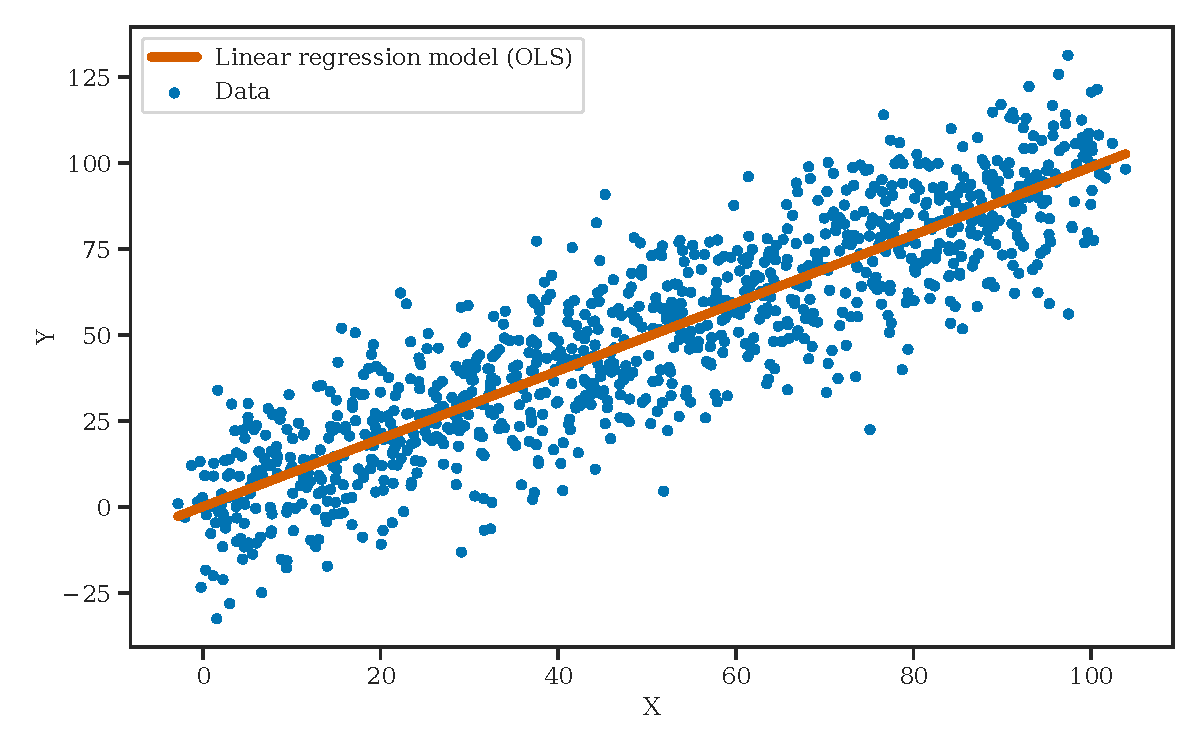
\includegraphics[width=0.7\textwidth]{thesis/figures/linear-regression-example.pdf}
    \caption{A linear regression model using OLS, with one dependent variable Y and one independent variable $X$. The red line shows the OLS model.}
    \label{fig:linear-regression-ols}
\end{figure}

So far, we have only looked at the simplest form of linear regression, namely only using a single independent variable $X$ to predict a value for $Y$. To generalize the linear regression to $k$ independent variables, we now assume that our training data has $k$ variables (which we also refer to as \textit{features} or \textit{columns}), i.e. $X \in R^{n \times d}$. Finally, we add the new columns from $X$ to the model matrix $X'$, by extending \cref{eqn:y-hat-two-matrix-form} as
\begin{align}
    \hat{Y} =
        \undertext{
        \begin{bmatrix}
            1 & x_{11} & \ldots & x_{1k} \\
            1 & x_{21} & \ldots & x_{2k} \\
            \vdots & \vdots & & \vdots \\
            1 & x_{n1} & \ldots & x_{nk} \\
        \end{bmatrix}
        }{$X'$}
        \undertext{
        \begin{bmatrix}
            \hat{\beta}_0 \\
            \hat{\beta}_1 \\
            \vdots \\
            \hat{\beta}_k \\
        \end{bmatrix}
        }{$\hat{\beta}$},
    \label{eqn:y-hat-matrix-form-general}
\end{align}
To estimate the model parameters $\hat{\beta}$, we compute them using \cref{eqn:ordinary-least-squares}. Furthermore, we generalize the minimization objective of OLS in \cref{eqn:RSS-ols-two-variables} to use $k$ independent variables as well, by computing
\begin{align}
    \text{RSS} = \sumlim{i=1}{n}{\enclb{y_i - \enclp{\hat{\beta_0} +  \sumlim{j=1}{k}{\hat{\beta_j}x_{ij}}}}^2}.
    \label{eqn:RSS-ols-k-variables}
\end{align}

\subsubsection{Lasso regression}
\label{sec:lasso-regression}
Linear regression suffers from the fact that it has to use all independent variables to predict a value for the dependent variable. Imagine that we gather some $5$-dimensional data $X$, and want to predict some quantity $y$ using $X$. We perform some analysis on the data and notice that two of the features of the data are plain noise and most likely does not help to predict $y$. \textit{Lasso regression} is a slight modification of linear regression that helps us with this problem. By adding a \textit{penalty term} on the model parameters in the objective of the linear regression, lasso regression can push certain features to 0, essentially "removing" them from the model. If we had two very similar features, the lasso is also able to "nullify" one of them, since the first one "explains" the second one. As a result, the models we get from lasso regression are generally much easier to interpret. What we have described here is also referred to as \textit{feature selection}, where the model automatically selects which variables are useful for prediction.

Lasso regression minimizes the residual sum of squares (RSS) plus some constant $\lambda$ times the \textit{$\ell_1$-norm} of the model parameters $\beta$. We define the minimization objective as
\begin{align}
    \sumlim{i=1}{n}{\enclb{y_i - \enclp{\hat{\beta_0} +  \sumlim{j=1}{k}{\hat{\beta_j}x_{ij}}}}^2} + \lambda ||\beta||_1 = \text{RSS} + \lambda ||\hat{\beta}||_1,
    \label{eqn:lasso-regression-objective}
\end{align}
where $\lambda \geq 0$ is a \textit{regularization} parameter. We denote the second term of \cref{eqn:lasso-regression-objective}, $\lambda ||\hat{\beta}||_1$, as the $\ell_1$-penalty, which is small when $\hat{\beta}_0$, $\hat{\beta}_1$, \ldots, $\hat{\beta}_k$ are small. When $\lambda = 0$, the penalty term has no effect and lasso regression produces the same result as standard linear regression. As $\lambda \rightarrow \infty$, the effect of the $\ell_1$-penalty grows and the model parameters $\hat{\beta}$ approaches zero, and in some cases, some of the model parameters are be exactly zero. We define the $\ell_1$-norm as $||\hat{\beta}||_1 = \sum |\hat{\beta}_j|$, where $|\cdot|$ is the absolute value.

\subsubsection{Logistic regression}
\label{sec:logistic-regression}
When describing linear regression models in \cref{sec:linear-regression}, we assume that the response variable $Y$ is \textit{quantitative}. When working with \textit{qualitative} data, on the other hand, linear regression fails to work. For example, colours are qualitative, taking on values such as blue, red, green or brown; we can not claim that red is greater than blue or brown is less than green (discarding RGB colour information). When we predict a qualitative response variable $Y$ using some data $X$, we perform what we call a \textit{classification} task. \textit{Logistic regression} is a method that can predict the response variable $Y$ when it falls into one of two categories (i.e. binary response). Examples of a binary response variable are "Yes"/"No", "Is a dog"/"Is not a dog" and the typical 0/1, which we commonly use in machine learning. Logistic regression creates a model that models the probability that $Y$ falls belong to a particular category. In \cref{fig:logistic-regression-example}, we further motivate the use of logistic regression for binary-response tasks and we see that linear regression is not well-suited for predicting values between 0 and 1.
\begin{figure}[H]
    \centering
    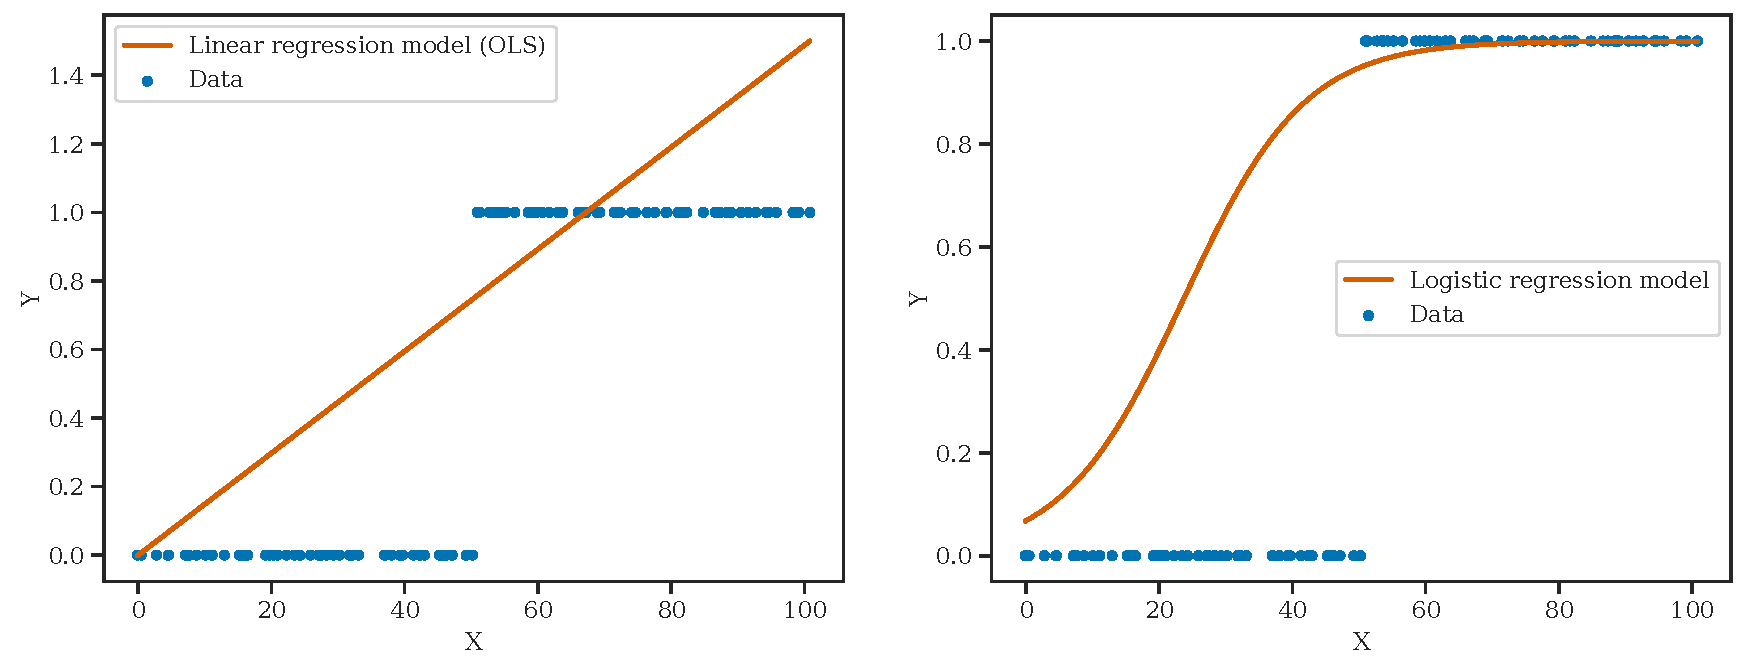
\includegraphics[width=\textwidth]{thesis/figures/logistic-regression-example.pdf}
    \caption{Illustration of linear and logistic regression models predicting some binary response variable $Y$ on data $X$. We see that logistic regression is particularly well-suited for predicting values for $Y$ between 0 and 1. Linear regression fails to model this relationship and even goes out of bounds for $X > 70$.}
    \label{fig:logistic-regression-example}
\end{figure}

Let $p(X) = Pr(Y = 1|X)$ denote the probability of $Y$ being 1 when we have the data $X$. If we want to model this relationship, we could use linear regression by
\begin{align}
    p(X) = \beta_0 + \beta_1 X.
\end{align}
Unfortunately, as mentioned earlier, linear regression is not a good fit for such problems and we would have the situation on the left of \cref{fig:logistic-regression-example}. In logistic regression, the \textit{logistic function} is used to ensure that the output value falls between 0 and 1, and we define it as
\begin{align}
    p(X) = \frac{\exp{\enclp{\beta_0 + \beta_1 X}}}{1 + \exp{\enclp{\beta_0 + \beta_1 X}}}.
    \label{eqn:logistic-function-p-x}
\end{align}
The plot to the right of \cref{fig:logistic-regression-example} shows the effect of the logistic function, creating an S-shaped like curve that for high $X$-values, creates values close to, but never greater than 1. On the other hand, the logistic function creates values close to, but lever less than 0 for low $X$-values. Manipulating \cref{eqn:logistic-function-p-x} a bit, we get that
\begin{align}
    \frac{p(X)}{1 - p(X)} = \exp{\enclp{\beta_0 + \beta_1 X}},
    \label{eqn:logistic-function-odds}
\end{align}
where we refer the left-hand-side of \cref{eqn:logistic-function-odds}, i.e. $p(X)/\enclb{1 - p(X)}$, as the \textit{odds}. As $p(X)$ increases, the odds increases exponentially towards $\infty$. Taking the logarithm of both sides of \cref{eqn:logistic-function-odds}, we finally arrive at
\begin{align}
    \log \enclp{\frac{p(X)}{1 - p(X)}} = \beta_0 + \beta_1 X,
    \label{eqn:logistic-function-logit}
\end{align}
where we refer the left-hand-side of \cref{eqn:logistic-function-logit} as the \textit{logit}. Thus, we see that the logistic regression model has a logit that is linear in $X$. If we increase $X$ by one unit, then the log odds increase by $\beta_1$. However, note that the relationship between $p(X)$ and $X$ in \cref{eqn:logistic-function-p-x} is not a straight line. For this reason, the amount of $p(X)$ changes due to a single unit change in $X$ depends on the current value of $X$. In \cref{fig:logistic-regression-example}, we see that once $X$ reaches a certain threshold (e.g. $X=30$), the rate at which $Y$ changes decreases towards zero.

If we would like to model logistic regression using multiple predictors, we only have to perform a simple extension from simple to multiple linear regression. We generalize \cref{eqn:logistic-function-logit} as
\begin{align}
    \log \enclp{\frac{p(X)}{1 - p(X)}}
    &= \beta_0 + \beta_1 X_1 + \beta_2 X_2 + \ldots + \beta_k X_k \label{eqn:logistic-function-logit-multiple} \\
    &= \beta_0 + \sumlim{i=1}{k}{\beta_i X_i}, \notag
\end{align}
where $X = \enclp{X_1, X_2, \ldots, X_k}$ are $k$ predictors.

To estimate the parameters $\beta_0, \beta_1, \ldots, \beta_k$ for $k$ predictors, it is common to use the \textit{maximum likelihood} method. We do not go into detail about the maximum likelihood method here, but kindly refer the reader to \cite[p. 214]{fox2015applied} for more details.

\subsection{Model selection}
\label{sec:model-selection}
\textit{Model selection} is an important aspect of modern machine learning. When working with machine learning, we would like to understand which model solves the problem the best, and model selection helps us with this. Model selection is the task of selecting a model for a particular problem using the data at hand. We look at a couple of methods for performing model selection, namely using train/validation/test splits and $K$-fold cross-validation. We refer to \cite{James2013} when describing model selection methods. Furthermore, we will use model selection when training lasso and logistic regression model for supervised word polysemy prediction in \cref{sec:analysis-of-embeddings-supervised-polysemy-prediction}.

\subsubsection{Train, validation and test splits}
\label{sec:train-val-test-splits}
When training a supervised machine learning model, we typically have some data $X$ and corresponding labels $y$. The task is to predict the labels $y$ using the data $X$. Since we do not know apriori which model or model parameters to use, the most common way to figure this out is by performing model selection. The simplest kind of model selection for machine learning models is to split the data $X$ and labels $y$ into three data sets, namely the \textit{train-}, \textit{validation-}, and \textit{test data sets}. The new data sets are chosen at random and do not overlap. An example of a train/validation/test split ratio could be 80/10/10, where we use 80\% of the data by the training, 10\% by the validation and 10\% by the test data set. Exactly how we split the data sets into the smaller train/validation/test data sets depends very much so on the application and how much data we are working with. In more modern machine learning models, e.g. using artificial neural networks, it is common to use up to 99\% of the data for training, as long as we have a big enough data set (e.g. $>1$ million data points).

We use the train data set to learn the models' parameters from the data, e.g. a linear regression models $\beta$ parameter. The train data set is usually much larger than the validation or test data sets. To evaluate the parameters of the model, we use the \textit{validation data set}. When we evaluate a trained model using a validation data set, we perform what we call the \textit{validation set approach}. The validation data set provides an unbiased estimate of a models' fit on the training data set while tuning some \textit{hyperparameter}. A hyperparameter is a parameter that we choose for the model beforehand, in contrast to a model parameter, which the model learns internally. Tuning hyperparameters can be a difficult task, especially if we have a lot of hyperparameters with various values. A typical way of performing hyperparameter optimization is by using \textit{grid search}, which tries out all combinations of all hyperparameter values. Grid search can be computationally expensive, especially if we would like to try out many choices of hyperparameters. For this reason, we typically use grid searches to find potential ranges where the optimal hyperparameters live and then narrow down the search for smaller ranges of hyperparameters to find more optimal ones.

After selecting a model or a set of model parameters using the validation data set, we use the test data set to give an unbiased estimate of how the model performs on unseen data. Additionally, we refer to the test data set as the \textit{hold-out data set}, because its only use is at the end of model selection. Note that we do not necessarily require to have a test data set available to perform model selection, as it only evaluates the performance of the final model. A common approach is also to exclude the test data set and instead split the original data $X$ into training and validation only. By doing so, we are unable to get an unbiased estimate of the models' performance on unseen data. We illustrate the process of splitting data into train/validation/test splits in \cref{fig:train-val-test-splits}.
\begin{figure}[H]
    \centering
    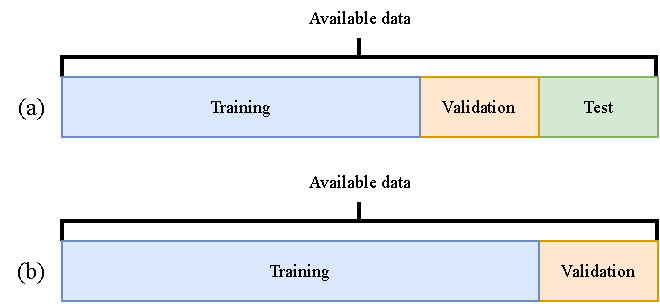
\includegraphics[width=0.9\textwidth]{thesis/figures/train-val-test-splits_cropped.pdf}
    \caption{Example of ways to partition a data set for model selection. The partition on the top (a) splits the data into training, validation and test, while the partition on the bottom (b) splits the data into training and validation only.}
    \label{fig:train-val-test-splits}
\end{figure}

The validation set approach is simple and works fine in practice. There are, however, a couple of drawbacks when using this method. Depending on which observations we include in the training and validation data sets, the validation estimate of the error can vary a lot. In addition to this, since the validation set approach only uses a subset of the observations to train the model, and the fact that statistical models perform worse when we train them on less data, the validation error rate tends to overestimate the test error rate of a model trained on the entire data set. In the next sub-subsection, we introduce $k$-fold cross-validation, an improvement over the validation set approach that addresses these two drawbacks.

\subsubsection{k-fold cross-validation}
\label{sec:cross-validation}
An alternative to the validation set approach is the \textit{$k$-fold cross validation} (CV) method. The $k$-fold CV method randomly divides the training data $X$ into $k$ groups, or \textit{folds}, of approximately equal size. We treat the first fold as the validation data set and train the model on the remaining $(k - 1)$ folds. We compute the validation error $\text{Err}_1$ on the first validation data set. Following, this procedure is repeated $k$ times, and for each time, we use a different group of data points from the original training data $X$ as the validation data. This results in $k$ estimates of the test error, i.e. $\text{Err}_1$, $\text{Err}_2$, \ldots, $\text{Err}_k$. We compute the total $k$-fold CV error estimate by taking the mean of these values, as
\begin{align}
    \text{CV}_k = \frac{1}{k} \sumlim{i=1}{k} \text{Err}_i.
\end{align}
Choosing a value for $k$ is a hard problem. The most common choice is to set $k=5$ or $k=10$, depending on the problem. We kindly refer the reader to \cite[Section 5.1.4]{James2013} for more details on choosing a value for $k$.

We show an illustrative example of $k$-fold CV in \cref{fig:k-fold-cv}, where we see a typical set-up when using a $k$-fold CV, namely to split all available data into training and test data sets. During the training process, the training data set is furthermore split into training and validation data sets for that particular $k$.
\begin{figure}[H]
    \centering
    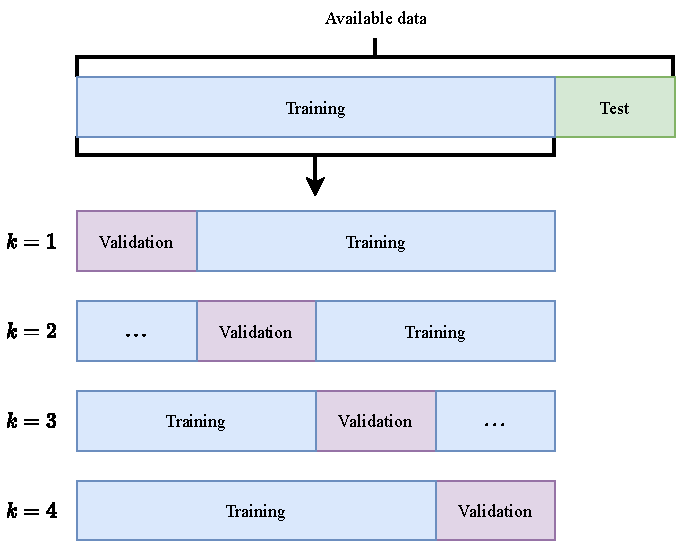
\includegraphics[width=0.9\textwidth]{thesis/figures/k-fold-cv_cropped.pdf}
    \caption{Data split into training and test data sets. To perform model selection, we use $k$-fold cross-validation. In this example, we have a $4$-fold cross-validation setting. As the $k$ increases, we have different data sets for both training and validation.}
    \label{fig:k-fold-cv}
\end{figure}

The benefit of using $k$-fold CV is that, by both training on different subsets of the training data and evaluating the model on different validation data sets, the estimated test error becomes more accurate and we get less varying results, as long as we select a good value for $k$.

\subsection{Performance metrics}
\label{sec:performance-metrics}
In this subsection, we introduce some common choices of performance metrics for regression and classification problems. We use performance metrics to evaluate machine learning models on data sets. In the following sub-subsections, we look at classification accuracy, the confusion matrix and sensitivity. Furthermore, we will use the performance metrics below to evaluate the word2vec model in \cref{sec:word2vec-model-evaluation} and for evaluating results from prediction of polysemous words in \cref{sec:analysis-of-embeddings-supervised-polysemy-prediction}.

\subsubsection{Classification accuracy}
\label{sec:classification-accuracy}
\textit{Classification accuracy} (which we also refer to as \textit{accuracy}) is the ratio between correct predictions to the total number of samples. We typically use classification accuracy in classification problems, as it is a simple and interpretable metric. Let $C_p$ be the number of correct predictions and let $N$ be the total number of samples. We compute classification accuracy as
\begin{align}
    \text{ACC}(C_p, N) = \frac{C_p}{N}.
    \label{eqn:classification-accuracy}
\end{align}
One pitfall of using classification accuracy is when we are dealing with classification problems with unbalanced data sets. Imagine that we want to compute the performance of a classification model for classifying whether or not a patient has a rare, but fatal disease. If we use classification accuracy, it is not common to get very high accuracies (e.g. $99.9\%$), when in reality, the number of correct classifications for whether or not a patient has the disease is significantly lower. In other words, we get a false sense of the models' performance. To deal with such cases, it is more common to use metrics such as sensitivity (see \cref{sec:sensitivity}), which deals with class imbalance much better and is well-suited for specific tasks.

\subsubsection{Confusion matrix}
\label{sec:confusion-matrix}
\textit{Confusion matrices} explains the performance of classification models by creating a matrix of predicted values to true labels. We see such a confusion matrix in \cref{fig:confusion-matrix}, where we have a binary classification problem (two classes; 0 and 1). As we see in \cref{fig:confusion-matrix}, we have four terms which describe the performance of the model, namely the \textit{True Negative} ($TN$), \textit{False Negative} ($FN$), \textit{False Positive} ($FP$) and \textit{True Positive} ($TP$) terms. $TN$ is the number of predicted negative classes when the true classes were negative, while on the other hand, $TP$ is the number of predicted positive classes when the true classes were positive. Off the diagonals of \cref{fig:confusion-matrix}, we see FP, which is the number of predicted positive classes when the true classes were negative, and FN, which is the number of predicted negative classes when the true classes were positive. When computing accuracy we would like, ideally, the number of $TN$ and $TP$ samples to be as high as possible and the number of $FN$ and $FP$ samples to be as low as possible. In cases where we have a high class imbalance (e.g. from example in \cref{sec:classification-accuracy}), it is more common to optimize either $TN$ or $TP$ to be as high as possible, effectively minimizing either $FN$ or $FP$. We look at one such metric, namely sensitivity in \cref{sec:sensitivity}.
\begin{figure}
    \centering
    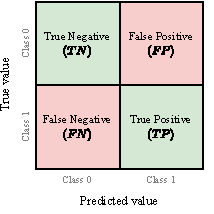
\includegraphics[width=0.5\textwidth]{thesis/figures/confusion-matrix_cropped.pdf}
    \caption{A typical example of a confusion matrix of a binary classification problem, with classes 0 and 1.}
    \label{fig:confusion-matrix}
\end{figure}

\subsubsection{Sensitivity}
\label{sec:sensitivity}
\textit{Sensitivity} is a performance metric which measures the ability of a classification model to correctly classify a positive class (e.g Class 1 in \cref{fig:confusion-matrix}). The sensitivity only focuses on the values where the true class is positive, i.e $FN$ and $TP$ for a binary classification problem. More formally, we define sensitivity as the portion of correctly predicted positive classes to the number of samples with a positive class. We compute the sensitivity as
\begin{align}
    \text{SEN} = \frac{TP}{TP + FN}.
    \label{eqn:sensitivity}
\end{align}
If we, on the other hand, would like to look at the ability of a classification model to correctly classify a negative class (e.g. Class 0 in \cref{fig:confusion-matrix}), we can, with minor modification of \cref{eqn:sensitivity}, change to focus on the prediction of negative classes. This modification creates a measure commonly referred to as \textit{specificity}.
\section{Word embeddings}
\label{sec:word-embeddings}
In this section, we will formulate the problem of creating efficient vectorized representations of text and explain methods for doing so. In particular, we will discuss ways of representing text numerically in \cref{sec:numerical-repr-of-text}, describe how we can create word embeddings and details around the word2vec method in \cref{sec:word2vec}, from architectural choices to presenting word2vec as an artificial neural network. Finally, we will introduce a couple of alternative models for learning word embeddings in \cref{sec:other-models-for-learning-word-embeddings} and explain how to evaluate word embedding models in \cref{sec:eval-word-embedding-models}.

\subsection{Numerical representation of text}
\label{sec:numerical-repr-of-text}
Machine learning methods take in vectors (arrays of numbers) as input. When we want to work with text, we have to come up with some procedure for converting text into a vector, i.e. vectorizing the text. In this subsection, we create unique representations for words in a text, discuss one-hot encoding of words and the motivation behind creating word embeddings.

\subsubsection{Unique representation for each word}
\label{unique-representation-for-each-word}
A first strategy for vectorizing text could be to assign a unique number for each word in the text. We use the same order as the words that appear in the text to assign a unique number. We call the set of unique words that appear in the text the \textit{vocabulary} and denote it as $V$. Furthermore, we define the number of unique words in the text to be the \textit{vocabulary size} and denote it as $|V|$. Finally, we replace each word in the text with its respective number. Let us consider an example of a (lower-cased) sentence, which we define as
\begin{align}
    S = \text{the cat sat on the mat}.
    \label{eqn:num-rep-ex-sent-words}
\end{align}

Following, we convert the words into numbers using the numerical order they appear in the text, e.g. the $\mapsto$ 0, cat $\mapsto$ 1, sat $\mapsto$ 2, etc. We convert the sentence in \cref{eqn:num-rep-ex-sent-words} to numbers as
\begin{align}
    S = \text{0 1 2 3 0 4}
    \label{eqn:num-rep-ex-sent}.
\end{align}
In \cref{eqn:num-rep-ex-sent}, we see a numerical representation of the original sentence in \cref{eqn:num-rep-ex-sent-words} and may use it for machine learning modeling. However, there are some problems with this method:
\begin{itemize}
    \item The encoding of words into number is arbitrary (does not capture any relationship between words)
    \item Machine learning models might learn some natural ordering of the encodings, which can lead to bad results during inference. This is because the encoding of the words does not capture the relationship between the words.
\end{itemize}

In the next sub-subsection, we look at another method for encoding words, using one-hot encodings. Furthermore, we apply it to the example sentence in \cref{eqn:num-rep-ex-sent-words}.

\subsubsection{One-hot encoded words}
\textit{One-hot encoding} is a method for converting categorical data into numeric data. Essentially, we create a unique, sparse vector consisting of all zeros, except for the value at the index of the element of interest, which we set to one. For instance, if we have the words "north", "east", "south", "west", then their one-hot encodings could be
\begin{align}
    \text{north} \mapsto \begin{pmatrix}
    1\\
    0\\
    0\\
    0
    \end{pmatrix},
    \text{east} \mapsto \begin{pmatrix}
    0\\
    1\\
    0\\
    0
    \end{pmatrix},
    \text{south} \mapsto \begin{pmatrix}
    0\\
    0\\
    1\\
    0
    \end{pmatrix},
    \text{west} \mapsto \begin{pmatrix}
    0\\
    0\\
    0\\
    1
    \end{pmatrix}.
\end{align}

Let the vocabulary $V = \left \{ w_1, w_2, ..., w_{|V|} \right \}$ to be the set of unique words in a text. Then, we define the one-hot encoding of a word, $e_{w_i}$, to be the $|V|$-dimensional vector of all zeros, except for the value at index $i$ which is one. Using the definition of one-hot encoding, we convert the words from the sentence in \cref{eqn:num-rep-ex-sent-words}. Precisely, we convert the sentence as
\begin{align}
    S = \begin{pmatrix}
    1\\
    0\\
    0\\
    0\\
    0
    \end{pmatrix}
    \begin{pmatrix}
    0\\
    1\\
    0\\
    0\\
    0
    \end{pmatrix}
    \begin{pmatrix}
    0\\
    0\\
    1\\
    0\\
    0
    \end{pmatrix}
    \begin{pmatrix}
    0\\
    0\\
    0\\
    1\\
    0
    \end{pmatrix}
    \begin{pmatrix}
    1\\
    0\\
    0\\
    0\\
    0
    \end{pmatrix}
    \begin{pmatrix}
    0\\
    0\\
    0\\
    0\\
    1
    \end{pmatrix},
    \label{eqn:one-hot-rep-ex-sent-words}
\end{align}
where we see that we discard the the ordinal relationship of the numerical representation in \cref{eqn:num-rep-ex-sent}. However, there are some downsides with this approach, as well:
\begin{itemize}
    \item As with the numerical representation in \cref{unique-representation-for-each-word}, one-hot encoded vectors does not capture the relationship between words.
    \item One-hot encoded vectors are sparse (meaning, most values are zero). Imagine if we had 1000 words in the vocabulary, then one would create a vector consisting of 99.9\% zeros. In practice, the vocabulary size is in the terms of $10^5$ to $10^7$ \cite{mikolov2013b}, i.e. by using one-hot encoded vector representations we are extremely inefficient in terms of space. We note, however, that there exist efficient methods for dealing with sparse vectors.
    \item One-hot encoded vectors are very high-dimensional (same as the number of words in the vocabulary, $|V|$).
\end{itemize}
In the next sub-subsection, we look at word embeddings, which solves many of the problems of the numerical representations presented so far.

\subsubsection{Word embeddings}
In comparison to the high-dimensional one-hot encoded vectors of words, \textit{word embeddings} are low-dimensional dense vector representations. Word embedding models learn their word embeddings from the data (e.g. texts) directly, whereas, for one-hot encoded vectors, we can arbitrarily define them (e.g. its ordering may change). Also, due to the lower dimensionality of word embeddings, it has to pack more information about words into less space. Moreover, word embeddings use all their dimensions to learn hidden relations and concepts of words, in contrast to one-hot encodings, which effectively only uses a single dimension (e.g. the position of the word in the vocabulary). Common choices for the dimensionality of word embeddings range from 50 to 600 \cite{mikolov2013a}, depending on the amount of training data. In the next subsection, we look at a classic family of methods for creating such word embeddings, namely word2vec.

\subsection{Learning word embeddings}
\label{sec:word2vec}
\textit{Word2vec} was first introduced by Mikolov et al. in 2013 \cite{mikolov2013a}. It is a family of methods for learning dense and efficient vector representations of words. In the same year, Mikolov et al. published a follow-up paper, \cite{mikolov2013b}, which includes several extensions that improve both the quality of the word embeddings and the training speed. In this subsection, we explain the details of the original word2vec paper, \cite{mikolov2013a}, and the introduced extensions in the follow-up paper, \cite{mikolov2013b}. We base this subsection on \cites{mikolov2013a}{mikolov2013b}. Furthermore, we will use the word2vec method to create word embeddings for the analysis in \cref{sec:training-and-eval-our-word2vec-impl}.

\subsubsection{Architectures}
The authors of the word2vec paper introduced two new log-linear models for learning distributed representations of words that try to minimize computational complexity, namely the \textit{continuous bag-of-words model} (CBOW) and the \textit{continuous Skip-gram model}. Both models achieve high quality (see \cref{sec:eval-word-embedding-models} for evaluation of word2vec models) word embeddings and share some core idea as to how we can create good vector representations of words. In this sub-subsection, we go through both models and explain the similarities and differences.

\paragraph*{Continuous bag-of-words model}\mbox{} \\
The continuous bag-of-words model (CBOW) tries to predict a target word given some context words around it. Essentially, we select a target word $w_t$, where $t$ is the index of the current target word in our training data, and a number $C$ denoting the number of words to the left and the right of $w_t$. We also refer to $C$ as the \textit{window size}. Let $S=2C$ denote the total number of words to the left and right. By combining the context word embeddings, we predict the target word $w_t$. We illustrate the CBOW model in \cref{fig:cbow-model}.
\begin{figure}[H]
    \centering
    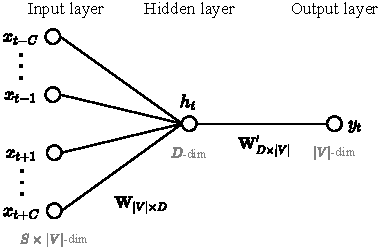
\includegraphics[width=11cm]{thesis/figures/cbow_cropped.pdf}
    \caption{An illustration of the CBOW architecture. The input value $x_{t+k}$ is the one-hot encoded vector of word $w_{t+k}$, where $k \in \enclc{-C, \ldots, -1, 1, \ldots, C}$, $t \in \enclc{1, \ldots, T}$ is training word position and $C$ is the window size. The output of CBOW is a $|V|$-dimensional vector $y_t$ of probabilities for sampling the target word $w_t$.}
    \label{fig:cbow-model}
\end{figure}

More formally, we are considering a sequence of $T$ training words $w_1, w_2, \ldots, w_T$. The words $w_t$ belong to some vocabulary $V$ consisting of $|V|$ unique words, $1 \leq t \leq T$. The models task is to maximize the average log probability of sampling the word $w_t$, given the context words $w_{t-C}, \ldots, w_{t-1}, w_{t+1}, \ldots, w_{t+C}$. The objective of the CBOW model then becomes
\begin{align}
    \frac{1}{T} \sumlim{t=1}{T} \log p(w_t | w_{t-C}, \ldots, w_{t-1}, w_{t+1}, \ldots, w_{t+C}).
    \label{eqn:cbow-objective-function}
\end{align}

Through it is not clear from the original authors of word2vec \cite{mikolov2013a, mikolov2013b}, we typically use two weight matrices, $W$ and $W'$, when setting up the word2vec model \cite{rong2016word2vec}. The first weight matrix, $W$, is a $|V| \times D$ matrix, mapping the input words (we typically represent them using one-hot encodings) to their internal word embeddings, where $|V|$ is the vocabulary size, and $D$ is the number of dimensions in the embedding layer. The second weight matrix, $W'$, is a $D \times |V|$ matrix mapping from the embedding layer to the output prediction. In practice, we use the first weight matrix $W$ as word embeddings, but we note that some models utilize both weight matrices (e.g. GloVe in \cref{sec:glove}).

\paragraph*{Continuous Skip-gram model}\mbox{} \\
The continuous Skip-gram model is very similar to CBOW, and in fact, the Skip-gram model tries to do the opposite; instead of predicting a target word given some context words, it tries to predict context words given some target word. We note that the ordering of the predicted context words does not matter. We illustrate the Skip-gram model in \cref{fig:skip-gram-model}.
\begin{figure}[H]
    \centering
    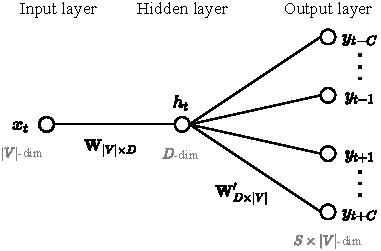
\includegraphics[width=11cm]{thesis/figures/skim-gram_cropped.pdf}
    \caption{An illustration of the Skip-gram architecture. The input value $x_t$ is the one-hot encoded vector of word $w_t$, where $t \in \enclc{1, \ldots, T}$ is training word position and $C$ is the window size. The output values are $|V|$-dimensional vectors $y_{t+k}$ of probabilities for sampling the word $w_{t+k}$, where $k \in \enclc{-C, \ldots, -2, -1, 1, 2, \ldots, C}$. We note that the ordering of the vectors from the output layers does not matter, as we only want to predict that a particular word belongs to its contextual words.}
    \label{fig:skip-gram-model}
\end{figure}

With the Skip-gram model, we also have some target word $w_t$ and context words around it. Let $C$ be the maximal distance from a target word to its contextual words. For each input to the model, we randomly sample a number $R$ in the range $[1, C]$ and denote this as the \textit{context size}. In other words, for each target word $w_t$ we have $R$ context words around it, $w_{t-R}, \ldots, w_{t-1}, w_{t+1}, \ldots, w_{t+R}$. The objective of the Skip-gram model then becomes
\begin{align}
    \frac{1}{T} \sumlim{t=1}{T} \sumlim{-R \leq j \leq R, j \neq 0}{} \log p(w_{t+j} | w_t).
    \label{eqn:skip-gram-objective-function}
\end{align}
More generally, we define the objective of the Skip-gram model as such
\begin{align}
    \frac{1}{T} \sumlim{t=1}{T} \sumlim{w_O \in cw(w_I)}{} \log p(w_O | w_I),
    \label{eqn:skip-gram-objective-function-general}
\end{align}
where $w_I$ is the input word (e.g. target word), $w_O$ is the output word (e.g. context word) and $cw(w_I)$ is a function which returns the context words around input word $w_I$.

Similar to CBOW, the Skip-gram model uses the two matrices $W$ and $W'$ for mapping from input to embedding layer and embedding layer to output respectively. Mikolov et al. report that the Skip-gram model performs better than the CBOW model overall, shown by their experiments in \cites{mikolov2013a}. For this reason, and due to the scope of the thesis, we will focus on the Skip-gram model. For the rest of the thesis, we refer to the weight matrix $W$ when talking about word embeddings of a word2vec model.

\subsubsection{Negative Sampling}
In the Skip-gram model, we typically compute $p(w_O | w_I)$ using the softmax function (see \cref{eqn:softmax-function}). More formally, we define it as
\begin{align}
    p(w_O | w_I)
    &= \frac{\exp{ \left( \trans{v'_{w_O}} v_{w_I} \right) }} {\exp{ \sumlim{k=1}{|V|} \left( \trans{v'_{w_k}} v_{w_I} \right) }},
    \label{eqn:skip-gram-p-function}
\end{align}
where $v_w$ and $v'_w$ are the "input" and "output" vector representations of the word $w$, and $|V|$ is the number of words in the vocabulary. There are some downsides with this formulation, however. In practice, it becomes hard to compute since the summation in the denominator of \cref{eqn:skip-gram-p-function} depends on the number of words in the vocabulary, which is often large ($10^5 - 10^7$ terms).

To deal with the computational requirements of the original Skip-gram model, \cite{mikolov2013b} first show that using \textit{hierarchical softmax}, we end up with a viable strategy. Hierarchical softmax is an efficient way of computing the softmax function; instead of evaluating $|V|$ words to compute the probability in \cref{eqn:skip-gram-p-function}, we only have to evaluate $\log \left( |V| \right)$ words.

As an alternative to hierarchical softmax, Mikolov et al. introduced \textit{negative sampling} in \cite{mikolov2013b}. Negative sampling builds on the concept of distinguishing target words $w_t$ from words randomly sampled from the vocabulary. In particular, we randomly sample words from the vocabulary using the \textit{unigram distribution} raised to the power of $\alpha$. The unigram distribution is a distribution used to sample random words from the vocabulary using the word occurrence counts. \cite{mikolov2013b} claim that by raising the unigram distribution to the power of $\alpha = 3/4$, we get the best result. Furthermore, we refer to this unigram distribution as the noise distribution $P_n(w)$. Note that we can also apply the negative sampling method to CBOW, but we leave these details out.

Before we can explain negative sampling, we define the positive and negative target-context pairs. Given a vocabulary $V$, a target word $w_t$ and the target words contextual words $w_{t-R}, \ldots, w_{t-1}, w_{t+1}, \ldots, w_{t+R}$ for some window size $R$, we define a \textit{positive target-context pair} to be the pair of the target word $w_t$ and a contextual word $w_{t+j}$, $-R \leq j \leq R, j \neq 0$, i.e. the pair $\left( w_t, w_{t+j} \right)$. Furthermore, we define a \textit{negative target-context pair} as the pair of the target word $w_t$ and a word $w_r$, i.e. the pair $\left( w_t, w_r \right)$. We randomly sample the word $w_r$ from the noise distribution $P_n(w)$.

To explain the idea of negative sampling, we look at how we compute the softmax loss, and in particular, how we only use a subset of all the words in the vocabulary. In particular, for each word in the text we are training on, we create a positive target-context pair $\left( w_t, w_{t+j} \right)$, $-R \leq j \leq R, j \neq 0$. Furthermore, we generate $k$ negative target-context pairs for each word, where $k$ is in the range of $5-20$ for small training sets and $2-5$ for big training sets. We let $W_{np} = \left \{ w_i | i \in 1, \ldots, k \right \}$ be the set of $k$ negatively sampled words from the noise distribution $P_n(w)$. With these details in mind, the objective of negative sampling becomes \cite{mikolov2013b, rong2016word2vec}
\begin{align}
    \log \sigma \left( \trans{v'_{w_O}} v_{w_I} \right) + \sumlim{w_i \in W_{np}}{} \log \sigma \left( -\trans{v'_{w_i}} v_{w_I} \right),
    \label{eqn:negative-sampling-obj-func}
\end{align}
where $\sigma$ is the sigmoid function (see \cref{eqn:sigmoid-function}), and $v_t$ and $v'_t$ are the "input" and "output" vector representations of the word $w$. Note that the objective in \cref{eqn:negative-sampling-obj-func} can be seen as a special case of the negative cross-entropy loss function. Furthermore, we replace every $\log p(w_O | w_I)$ in the original Skip-gram objective function of \cref{eqn:skip-gram-objective-function-general} by the objective in \cref{eqn:negative-sampling-obj-func}. As such, we define the objective of the Skip-gram model with negative sampling as
\begin{align}
    \frac{1}{T} \sumlim{t=1}{T} \sumlim{w_O \in cw(w_I)}{} \log \sigma \left( \trans{v'_{w_O}} v_{w_I} \right) + \sumlim{w_i \in W_{np}}{} \log \sigma \left( -\trans{v'_{w_i}} v_{w_I} \right).
    \label{eqn:skip-gram-negative-sampling-objective}
\end{align}
In \cref{eqn:negative-sampling-obj-func}, we see that we only have to compute for $(1 + k)$ words, which is a big improvement over computing for $|V|$ words (assuming that $|V|$ is much larger than $k$). \cites{mikolov2013b} also report that by using negative sampling, we increase the quality of the word embeddings.

\subsubsection{Subsampling of words}
When training a word2vec model, we typically have to train on big text corpora to achieve high-quality word embeddings. However, as the number of training words increases, the discrepancy between rare and frequent words increase as well. When using negative sampling, we are sampling negative target-context pairs from the vocabulary, which depends on the unigram distribution. In English text corpora, words such as "the", "of", "is" can easily occur hundreds of millions of times and usually provide less information than more rare words. For this reason, we apply a simple, yet efficient subsampling scheme to counter the imbalance between rare and frequent words; before we process the text corpora into target-context pairs, we discard each word $w_t$ with a \textit{discard probability} \cite{mikolov2013b, levy-etal-2015-improving}. We define the discard probability as
\begin{equation}
    P_d(w_t) = 1 - \sqrt{\frac{t}{f(w_t)}},
\end{equation}
where $f(w_t)$ is the (relative) frequency of word $w_t$ and $t$ is a chosen threshold, usually around $10^{-5}$.

We note, however, that in the original source code of word2vec \cite[line 407]{Word2vecCCode}, they use a slightly modified formula. We define the modified formula as 
\begin{align}
    P_d(w_t) = \frac{f(w_t) - t}{f(w_t)} - \sqrt{\frac{t}{f(w_t)}}.
    \label{eqn:discard-probability-impl}
\end{align}
Furthermore, we will use subsampling of words when implementing word2vec in \cref{sec:training-and-eval-our-word2vec-impl}, and in particular, we will use \cref{eqn:discard-probability-impl} for computing the discard probability.

\subsubsection{Learning word embeddings for phrases}
\label{sec:learning-word-embeddings-for-phrases}
Phrases are groups of words that occur frequently together, such as "New York" or "programming languages". Naturally, we would like to combine such words into a single token, such that word embedding models can learn them. To learn word embeddings for phrases, \cite[4 Learning Phrases]{mikolov2013b} propose a simple, yet efficient data-driven approach, where they combine phrases using their word counts. In particular, we define the phrase score for two words $w_i$ and $w_j$ as
\begin{align}
    \text{score}(w_i, w_j) = \frac{\text{freq}(w_i, w_j) - \delta}{\text{freq}(w_i) \cdot \text{freq}(w_j)},
    \label{eqn:word2phrase-score}
\end{align}
where $w_i$ and $w_j$ are bigrams, or two neighbouring words, from the vocabulary, $freq()$ returns the how many times the word (or bigram) occurs in the vocabulary and $\delta$ is a hyperparameter for preventing long phrases consisting of infrequent words from appearing. We refer to this phrase-learning procedure as \textit{word2phrase}, as specified by the original source code \cites{Word2phraseCCode}. If the score in \cref{eqn:word2phrase-score} is above the $\delta$ threshold hyperparameter, we accept the bigram into the vocabulary and we replace all occurrences of the two words $w_i$ and $w_j$ where they are next to each other. We use word2phrase to convert phrases into single words when preprocessing data for training our word2vec model in \cref{sec:word2vec-data-preprocessing}.

\subsubsection{Word2vec as an artificial neural network}
\label{sec:word2vec-as-an-ann}
Typically in the literature, word2vec is presented using the \cref{eqn:cbow-objective-function,eqn:skip-gram-p-function,eqn:negative-sampling-obj-func}. However, we explain how to set word2vec up as an artificial neural network (ANN, \cref{sec:artificial-neural-networks}), in the sense that we implement it later in the thesis (see \cref{sec:training-and-eval-our-word2vec-impl}). In particular, we explain how to set up the Skip-gram model with negative sampling as an ANN. This ANN consists of three fully-connected layers of artificial neurons \cite{rong2016word2vec}, and we illustrate it in \cref{fig:word2vec-skip-gram-negative-sampling}. The ANN we explain below acts as a baseline when implementing word2vec in \cref{sec:word2vec-impl-specifics}.

\begin{figure}[ht]
    \centering
    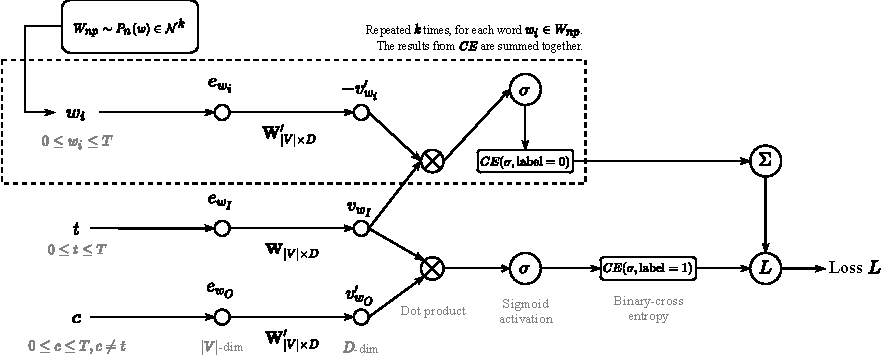
\includegraphics[width=16cm]{thesis/figures/word2vec-sgns_cropped.pdf}
    \caption{The artificial neural network architecture of word2vec Skip-gram model with negative sampling. The inputs to the network are $t$ and $c$, i.e, index of target word $w_t$ and context word $w_c$ in the vocabulary. For each forward pass in the network we sample $k$ word indices from $P_n(w)$. Furthermore, we use the $k$ sampled word indices to compute the negative sampling loss $L$.}
    \label{fig:word2vec-skip-gram-negative-sampling}
\end{figure}

\paragraph*{Input layers}\mbox{} \\
We have two input layers in our ANN; one for the target word $w_t$ and one for the context word $w_{t+j}$, $-R \leq j \leq R, j \neq 0$. The values to the input layers are typically one-hot encoded or represented using an integer corresponding to the index of the word in the vocabulary. For explanation purposes, we use the one-hot encoded representation here, but in our code implementation, we will use the latter one. We denote the input layers to be $\enclc{e_{w_t}}$ for the target word $w_t$ and $\enclc{e_{w_{t+j}}}$ for the context word $w_{t+j}$. Each of the input layers has $|V|$ values, where $|V|$ is the size of the word vocabulary.

\paragraph*{Hidden layer}\mbox{} \\
We have one hidden layer for each input layer in our ANN. To calculate the result from the input layers to its hidden layer, we introduce two $D \times |V|$ weight matrices $W$ and $W'$, where $D$ is the hidden embedding dimension and $|V|$ is the vocabulary size. The $W$ matrix consists of weights related to the target word $w_t$ and can be thought of as the "input to hidden" matrix. The $W'$ matrix consists of weights related to the context word, and unlike the $W$ matrix, it can be thought of as the "hidden to output" matrix from the original introduction to negative sampling. Note that we initialize both $W$ and $W'$ at random. Furthermore, we refer to $W$ and $W'$ as the target and context embedding matrix, respectively.

To map from the input to the hidden layer, we use a linear activation function (i.e. $id(x) = x$) with no bias, leading to more efficient training of bigger datasets. In other words, we simply multiply the embedding matrix (either $W$ or $W'$) with its respective one-hot encoded input vector, resulting in a "look-up" of the embedding vector. To illustrate with an example, imagine if we had the one-hot encoded vector $e_{w_t} = \left( \begin{smallmatrix}
    1\\
    0\\
\end{smallmatrix} \right)$ and the embedding matrix $W = \trans{\left( \begin{smallmatrix}
    1 & 2 & 3\\
    4 & 5 & 6\\
\end{smallmatrix} \right)}$. If the multiply the embedding matrix with the one-hot encoded vector, i.e. $W \cdot e_{w_t}$, we would get $\trans{\left( \begin{smallmatrix}
    1 & 2 & 3\\
\end{smallmatrix} \right)}$, essentially performing a "copy" operation. We let $\enclc{v_{w_t}} = W \cdot \enclc{e_{w_t}}$ be the hidden layer for word $w_t$ and $\enclc{v'_{w_{t+j}}} = W' \cdot \enclc{e_{w_{t+j}}}$ be the hidden layer for word $w_{t+j}$. 

\paragraph*{Output layer}\mbox{} \\
Recall that when we are using negative sampling, we would like to ensure that words in the same context yield similar word embeddings, and that words that are not in the same context (i.e. a target word versus a word sampled from the noise distribution $P_n(w)$) to be dissimilar. From the objective of negative sampling in \cref{eqn:negative-sampling-obj-func}, we see that we use the sigmoid function on the dot product between the "input" and the "output" vectors $v$ and $v'$ (in our setting: $\enclc{v_{w_t}}$ and $\enclc{v'_{w_{t+j}}}$). When we take the dot product, we are essentially computing an unnormalized cosine similarity measure between the vectors (we come back to the use of cosine similarity in \cref{sec:eval-word-embedding-models}). The core idea is to use this dot product similarity measure and convert it into the range of $[0, 1]$ by using the sigmoid function. Particularly, we want similar vectors to have 1 as output from the sigmoid function and dissimilar vectors to have 0 as the output from the sigmoid function. When we compute the loss of the ANN, we generate $k$ samples from the noise distribution $P_n(w)$ such that we can use them for computing the loss of the network.

For each positive target-context pair we have in our data, we create a single sigmoid output plus $k$ sigmoid outputs for each negative word we sample from the noise distribution $P_n(w)$. Thus, we could argue that we have $(k + 1)$ outputs in our network.  We note that, however, our main interest is to learn the internal embedding matrix $W$; we do not use the ANN for predicting whether a certain word is more or less likely to be within its contextual neighbourhood, thus, discarding the output of the network.

Similar to \cite{mikolov2013a}, we update the embedding weights $W$ and $W'$ using the stochastic gradient descent optimizer (see \cref{sec:ann-optimizers}), adjusting all the weights of the embedding matrices during the training of the ANN to minimize the loss in \cref{eqn:skip-gram-negative-sampling-objective}. Furthermore, we use a linearly decreasing learning rate, meaning that we start with some initial learning rate $lr$ and decrease linearly to $lr_{min}$ until we reach the end of training. The linearly decreasing learning rate is also used by \cite{mikolov2013a}.

\subsubsection{Hyperparameters in word2vec}
When training a word2vec model, we have to choose several hyperparameters. In this sub-subsection, we go over all choices of hyperparameters and explain them. We will explain the specific choices of hyperparameters that we use to train a word2vec model in \cref{sec:word2vec-hyperparameter-choices}.

\begin{itemize}
    \item \textbf{min-word-count} \\
        The minimum word count denotes a threshold of how many times a word at least has to occur in a text for it to be in the vocabulary. In the empirical experiments of Mikolov et al, they used 5 as the threshold.
    \item \textbf{max-vocab-size} \\
        The maximum vocabulary size denotes the maximal number of words to have in our vocabulary; we use the top \textbf{max-vocab-size} most common (i.e frequent) words. We may set the maximum vocabulary size to reduce the computational complexity and to remove some less occurring words.
    \item \textbf{batch-size} \\
        Batch size is the number of positive target-context pairs $(w_t, w_{t+j})$ we train on in each training step, i.e. the number of forward passes we perform in our ANN before we do a backwards pass.
    \item \textbf{num-epochs} \\
        The number of epochs denotes the number of times we train on the training data. With word2vec, we typically set this number rather low (e.g. $1-5$), as \cites{mikolov2013a} reports that by training on more data, we require fewer epochs to get comparable or better quality word embeddings.
    \item \textbf{learning-rate} \\
        The learning rate denotes how fast we want our weights to change in our ANN. The original authors of word2vec used 0.025 (i.e. $2.5\%$) as the initial learning rate for their experiments.
    \item \textbf{min-learning-rate} \\
        The minimal learning rate denotes how small the learning rate should be when approaching the end of the training. Mikolov et al. stated that they decreased it linearly, such that it approaches zero at the end of the last training epoch. We note, however, that in the original code of word2vec, they linearly decrease the learning rate to the initial learning rate $lr$ times $0.0001$ (i.e. $0.025 \times 0.0001 = 0.0000025$) \cite[line 398]{Word2vecCCode}.
    \item \textbf{embedding-dim} \\
        The embedding dimension denotes the dimension we want to use for the internal matrices $W$ and $W'$ in our ANN, i.e. the dimensionality of the word embeddings.
    \item \textbf{max-window-size} \\
        Maximum window size denotes the maximal number of words to look for to the left and the right of a target word $w_t$. Mikolov et al. reported that they used $5$ as the window size.
    \item \textbf{num-negative-samples} \\
        The number of negative samples denotes how many negative samples we generate for each positive target-context pair we train on.
    \item \textbf{sampling-factor} \\
        We use the sampling factor as a threshold to randomly discard frequently occurring words in the text corpora. A common value for this is $10^{-5}$.
    \item \textbf{unigram-exponent} \\
        The unigram exponent is which power we raise the noise distribution $P_n(w)$ to (where the noise distribution equals the unigram distribution, in our case). Although there was no theoretical justification for this, Mikolov et al. reported that the value $3/4$ worked the best.
\end{itemize}

\subsection{Other models for learning word embeddings}
\label{sec:other-models-for-learning-word-embeddings}
Creating word embeddings is a task that can be achieved in various ways. In this subsection, we briefly introduce two different models for computing word embeddings. The first model is the Global Vectors (GloVe) \cite{pennington2014glove} model. GloVe learns vector representations for words in a more "explicit" fashion than word2vec for example; we come back to this in \cref{sec:glove}. The second model is the fastText \cite{bojanowski2017enriching} model, which is an extension of the original word2vec Skip-gram model to include sub-word information. Note that we primarily focus on word2vec using Skip-gram with negative sampling in this thesis, and for this reason, we not go into depth when explaining GloVe and fastText. We use word embeddings from pre-trained GloVe and fastText models later in the analysis in \cref{sec:analysis-of-embeddings-topological-polysemy}.

\subsubsection{GloVe}
\label{sec:glove}
\textit{Global Vectors} (GloVe) \cite{pennington2014glove} is a model for learning vector representations for words. In contrast to word2vec, GloVe trains on the word to word co-occurrence counts, and thus, makes efficient use of statistics. In addition to this, the objective of GloVe is more explicit, as opposed to the vector representations word2vec learns, which are merely a by-product of the training. We base this sub-subsection on \cite{pennington2014glove}.

To understand how GloVe works, we first introduce the notion of the \textit{word to word co-occurrence matrix}, which we denote $X$. $X$ is a square matrix where each element $X_{ij}$ represent the number of times word $j$ occurs in the context of word $i$. Following, let $|V|$ denote the number of unique words in the vocabulary and let $X_i=\sumlim{k=1}{|V|} X_{ik}$ be the number of times any word appears in the context of word $i$. Using $X_{ij}$ and $X_i$, we can establish a probabilistic model $P_{ij}$ of how often a given word $j$ falls in the context of word $i$. Finally, we let $P_{ij}=P(j|i)=X_{ij} / {X_i}$. To motivate the use of $P_{ij}$, imagine that we want to investigate the concept of temperatures, which we extract directly from the co-occurrence probabilities. Consider the words $i = \text{sunny}$ and $j = \text{cloudy}$. We can explore relationships of the words $i$ and $j$ by studying the ratios of the co-occurrence probabilities with various other words, $k$. If we set the word $k = \text{hot}$, we expect the ratio $P_{ik} / P_{jk}$ to be large, since intuitively, the word "heat" is more related to the word "sunny" than the word "cloudy". If the word $k$ is set to an unrelated word of both sunny and cloudy, the ratio should be around 1, as both probabilities become rather low. The authors of \cite{pennington2014glove} give an example of studying the ratios of co-occurrence probabilities and is the foundation of how GloVe incorporates word count statistics to learn vector representations.

To learn vector representations of words, Glove uses two weight matrices, which we denote $W=\enclc{w_1, w_2, \ldots, w_{|V|}} \in \R^{|V| \times d}$ and $\Tilde{W}=\enclc{\Tilde{w}_1, \Tilde{w}_2, \ldots, \Tilde{w}_{|V|}} \in \R^{|V| \times d}$, similar to word2vec. That is, the weight matrix $W$ represents the target word embeddings, while $\Tilde{W}$ represent the context word embeddings. Furthermore, the objective function of GloVe consists of a weighted squared loss $J$ and we define it as
\begin{align}
    J = \sumlim{i, j = 1}{|V|} f \enclp{X_{ij}} \enclp{\trans{w_i} \Tilde{w}_j + b_i + \Tilde{b}_j - \log X_{ij}}^2,
    \label{eqn:glove-loss}
\end{align}
where $f$ is a weighting function, $b_i$ is bias for $w_i$ and $\Tilde{b}_j$ is bias for $\Tilde{w}_j$. The authors of GloVe found a particular class of functions for $f$ which was suitable, which we compute as
\begin{align}
    f(x) = \begin{cases}
        \enclp{x / x_{\text{max}}}^\alpha & \mbox{if } x < x_{\text{max}} \\
        1 & \text{otherwise}
    \end{cases},
    \label{eqn:glove-loss-f-function}
\end{align}
where $\alpha$ and $x_{\text{max}}$ are hyperparameters. In the experiments performed in \cite{pennington2014glove}, the authors let $x_{\text{max}}=100$ and $\alpha=3/4$. Furthermore, to train the GloVe model, they iteratively learn the weights over time in a gradient descent fashion, using AdaGrad \cite{Duchi2011} in particular, with an initial learning rate of $0.05$. Lastly, GloVe uses the sum of its weight matrices, i.e. $W + \Tilde{W}$, as the word embeddings, which the authors claim to lead to a minor increase in performance.

\subsubsection{fastText}
\label{sec:fasttext}
\textit{fastText} is an extension the word2vec Skip-gram model with negative sampling \cite{bojanowski2017enriching}. In particular, fastText represent each word using character $n$-grams, i.e. sub-words of length $n$ (e.g. $\textit{que}$ is a $3$-gram of the word $\textit{quest}$). We associate vector representations to each character $n$-gram, and following, we vectorize words using the sum of such representations. By creating vector representations of character $n$-grams, fastText can create representations for words that are not in the training vocabulary. We base this sub-subsection on \cite{bojanowski2017enriching}.

Recall the objective function of the Skip-gram model with negative sampling, which we show in \cref{eqn:skip-gram-negative-sampling-objective}. The authors of fastText generalize it by replacing the dot product between word embeddings with a scoring function $s(w_I, w_O) \mapsto \R$. We generalize \cref{eqn:skip-gram-negative-sampling-objective} using scoring function $s$ and define it as
\begin{align}
    \frac{1}{T} \sumlim{t=1}{T} \sumlim{w_O \in cw(w_I)}{} \log \sigma \left( s(w_I, w_O) \right) + \sumlim{w_i \in W_{np}}{} \log \sigma \left( -s(w_I, w_i) \right),
    \label{eqn:skip-gram-negative-sampling-objective-general}
\end{align}
where $s(w_I, w_O)=\trans{v'_{w_O}} v_{w_I}$ for the Skip-gram model with negative sampling.

As we mention in the introduction of this sub-subsection (see \cref{sec:fasttext}), fastText vectorizes each word $w$ using the vector representation of its character $n$-grams. To indicate the start and end of a word, we use the characters $<$ and $>$, respectively. We do this such that that the model can distinguish between prefixes and suffixes of words. Now, to give an example, let $w=\text{carbon}$ and $n=3$. We represent the word $w$ by character $n$-grams:
\begin{align*}
    \textless\text{ca}, \text{car}, \text{arb}, \text{rbo}, \text{bon}, \text{on}\textgreater,
\end{align*}
in addition to the word itself $\textless\text{carbon}\textgreater$. Note that the $n$-gram $\textless\text{car}\textgreater$, from the word car, is different from the $n$-gram car of the word $w$, due to the prefix and suffix characters. Furthermore, let $\mathcal{G}_w \subset \enclc{g_1, g_2, \ldots, g_G}$ be the set of $n$-grams appearing in word $w$, where $G$ is the total number of $n$-grams of all words in the vocabulary. We associate a vector $z_g$ to each entry $g$ in $\mathcal{G}_w$. The goal of fastText is to represent each word embedding as a sum of its $n$-grams, and consequently, we obtain the scoring function $s$. We define the scoring function $s$ as
\begin{align}
    s(w_I, w_O) = \sumlim{z_g \in \mathcal{G}_{w_I}}{} \trans{z_g} v_{w_O}.
    \label{eqn:fasttext-scoring-function}
\end{align}
This minor change to the scoring function allows the fastText model to share vector representations of $n$-grams between words, and thus, allow to learn more accurate representations for rare words (i.e. words that occur rarely in the training vocabulary).

Similar to the training of word2vec, the authors of fastText use stochastic gradient descent on the objective function in \cref{eqn:skip-gram-negative-sampling-objective-general} with \cref{eqn:fasttext-scoring-function} as scoring function. For more details of the training process, we kindly refer the reader to \cite[p. 3-4]{bojanowski2017enriching}.

\subsection{Evaluating word embedding models}
\label{sec:eval-word-embedding-models}
In typical machine learning projects, we commonly set aside some portion of the data, e.g. the test data set, and then use this data to evaluate the unbiased performance of models. In word embedding models, however, we do not follow this kind of practice. Instead, we evaluate the quality of the word embeddings on test data sets that measure word relatedness, as our interest lies in how well the word embeddings relate to each other. An example of a word relatedness test could be to check whether or not the word \textit{Oslo} is related to \textit{Norway} as the word \textit{Rome} is related to \textit{Italy}. In practice, however, for such word relatedness tests, we do not know the word \textit{Italy} (i.e. we hide it), and we must guess it from the entire vocabulary. By accumulating several word relatedness tests, we can create test sets, which we refer to as \textit{analogy data sets}. More generally, analogy data sets consists of questions to check whether or not a word \textit{A} is related to \textit{B} as \textit{C} is related to \textit{D}. By vectorizing the words, we want the differences between each pair of vectorized words to be roughly equal, and we show this relation as
\begin{align}
    v_{\textit{B}} - v_{\textit{A}} \approx v_{\textit{D}} - v_{\textit{C}}.
    \label{eqn:word-embedding-model-eval-relation}
\end{align}
Solving \cref{eqn:word-embedding-model-eval-relation} for $v_{\textit{D}}$, we get that
\begin{align}
    v_{\textit{D}} \approx v_{\textit{B}} - v_{\textit{A}} + v_{\textit{C}}.
    \label{eqn:word-embedding-model-eval-relation-wrt-d}
\end{align}
Now, since $v_{\textit{D}}$ is "hidden" from the model, we have to find a way of searching for the closest word matching the right-hand-side of \cref{eqn:word-embedding-model-eval-relation-wrt-d}. To do so, we often use cosine similarity, both for analogy tasks and measuring the distance between any two word embeddings. Let $u$ and $v$ be two vectors of the same size. We define the dot product between the vectors $u$ and $v$ as
\begin{align}
    u \cdot v = ||u||\,||v|| \cos\enclp{\theta},
    \label{eqn:u-v-dot-product}
\end{align}
where $||\cdot||$ is the magnitude (length) of the vector and $\cos \enclp{\theta}$ is the cosine of the angle $\theta$ between $u$ and $v$, which we refer to as the \textit{cosine similarity}. By solving for $\cos \enclp{\theta}$ in \cref{eqn:u-v-dot-product}, we get
\begin{align}
    \cos\enclp{\theta} = \frac{u \cdot v}{||u||\,||v||}.
    \label{eqn:cosine-similarity}
\end{align}
Thus, we see that by computing the cosine similarity of two vectors $u$ and $v$, we discard their magnitude, and thus, both vectors both have unit length. The removal of the vector magnitude is important, as we would like to compare vectors using vector addition and subtraction, as motivated by \cref{eqn:word-embedding-model-eval-relation}. Using cosine similarity, we can find the closest matching word embedding $v_{\textit{D}}$ (and associated word \textit{D}) by computing
\begin{align}
    v_{\textit{D}} = \argmax_{v_{\Tilde{\textit{D}}} \in W^*} \enclp{\cos \enclp{v_{\Tilde{\textit{D}}}, v_{\textit{B}} - v_{\textit{A}} + v_{\textit{C}}}},
\end{align}
where $W^*$ are the word embeddings $W$ in which we exclude the word embeddings $v_{\textit{A}}$, $v_{\textit{B}}$ and $v_{\textit{C}}$. It is common to exclude the vectors $v_{\textit{A}}$, $v_{\textit{B}}$ and $v_{\textit{C}}$ from the search, as \cite{mikolov2013a} did in their experiments.

Many machine learning algorithms require us to use Euclidean distance for comparing distances between vectors. To convert from cosine similarity to Euclidean distance, we observe that there is a relationship between the two vectors $u$ and $v$. We show this relationship as
\begin{align}
    ||u - v||_2^2 = \trans{(u - v)} (u - v) = ||u||^2 + ||v||^2 + 2\trans{u}v,
    \label{eqn:eval-word-embeddings-u-v-relationship}
\end{align}
where $||\cdot||_2^2$ is the squared Euclidean distance. Let $||u|| = ||v|| = 1$, i.e the vectors $u$ and $v$ are of unit length, then \cref{eqn:eval-word-embeddings-u-v-relationship} becomes
\begin{align}
    ||u - v||_2^2
    &= \trans{(u - v)} (u - v) \\
    &= 2 + 2\trans{u}v \notag \\
    &= 2(1 + \trans{u}v) \notag \\
    &= 2(1 + \cos \enclp{u, v}). \notag
\end{align}
In other words, we see a clear relationship between the squared Euclidean distance and cosine similarity. Some machine learning algorithms are applicable using dot-product as the distance metric, and by an expansion of \cref{eqn:cosine-similarity}, we see a particular relationship for unit-length vectors $u$ and $v$, namely that
\begin{align}
    \cos\enclp{\theta} = u \cdot v.
\end{align}
Furthermore, by using normalized word embeddings, we may use (squared) Euclidean distance or dot-product to emulate cosine similarity, as we get the same distance ranking by using cosine similarity. Lastly, we define the \textit{cosine distance} to be $(1 - \cos\enclp{\theta})$. We use the cosine distance in algorithms for measuring the distances between word embeddings. Furthermore, we will use cosine similarity when evaluating word embeddings models in \cref{sec:word2vec-model-evaluation}.
\section{Topological data analysis}
\label{sec:topological-data-analysis}
\textit{Topological Data Analysis} (TDA) is a fast growing field of mathematics, providing a set of tools from topology in order to infer underlying features from data \cite{chazal2021introduction}. In this section, we go over the concepts of TDA, such as simplicial complexes or persistence diagrams. Then, we introduce a couple of algorithms which uses concepts from TDA. We base this section on \cites{Edelsbrunner2010}{chazal2021introduction}, we do not if not state otherwise.

\subsection{Simplicial complex}
\label{sec:simplicial-complex}
In computer science, a \textit{graph} is a datatype for describing possibly non-linear and complex relationships between data points. In particular, graphs consist of vertices and edges, where the edges connect the vertices. Edges can also have metadata such as weight and direction. A common graph to use (in the context of computer science) is the $k$-nearest neighbour graph, where vertices are data points and edges represent neighbouring relationships, with distance as weight. A \textit{simplicial complex} is a generalization of graphs and we see its particular usage in TDA, due to its topological properties. Simplicial complexes consist of \textit{$n$-simplices}, where $0$-simplices are similar to vertices, $1$-simplices are similar to edges. The difference between graphs and simplicial complexes occur when we look at $n$-simplices for $n \geq 2$. For example, $2$-simplices form triangles and $3$-simplices form tetrahedrons (i.e. triangular pyramids). We show examples of $n$-simplices in \cref{fig:n-simplices-example}.
\begin{figure}[H]
    \centering
    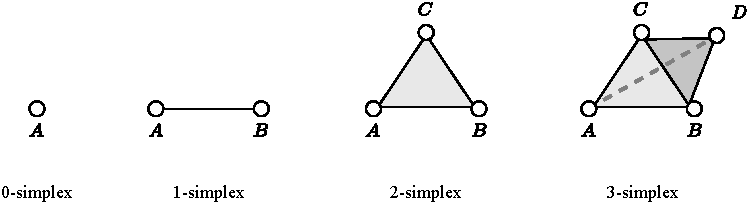
\includegraphics[width=0.9\textwidth]{thesis/figures/n-simplices_cropped.pdf}
    \caption{Building blocks of simplicial complexes, consisting of $n$-simplices.}
    \label{fig:n-simplices-example}
\end{figure}
By combining one or more $n$-simplices, we form simplicial complexes. We illustrate an example of a simplicial complex in \cref{fig:simplicial-complex}.
\begin{figure}[H]
    \centering
    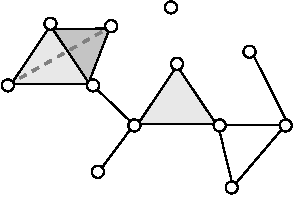
\includegraphics[width=0.5\textwidth]{thesis/figures/simplicial-complex_cropped.pdf}
    \caption{Simplicial complex consisting of $0$-, $1$-, $2$- and $3$-simplices.}
    \label{fig:simplicial-complex}
\end{figure}
There exist several methods for creating simplicial complexes from data. In particular, we look at one such simplicial complex in the next sub-subsection, namely the Vietoris–Rips complex.

\subsubsection{Vietoris–Rips complex}
\label{sec:vietoris-rips-complex}
The \textit{Vietoris–Rips complex} is a simplicial complex that we create from data points using any distance metric. Let $\alpha$ be a \textit{proximity diameter}. We build the Vietoris–Rips complex by forming a simplex for every set of $k$ data points that have distance less than or equal to $\alpha$. That is, if $k$ data points satisfy $d(x_i, x_j) \leq \alpha$ (where $d(x_i, x_j)$ computes the distance between two data points $i$ and $j$), we create a $(k-1)$ simplex for that particular data point (1-simplex for two data points, 2-simplex for three data points, etc.). We illustrate with an example of a Vietoris–Rips complex in \cref{fig:simplicial-complex-rips}.
\begin{figure}[H]
    \centering
    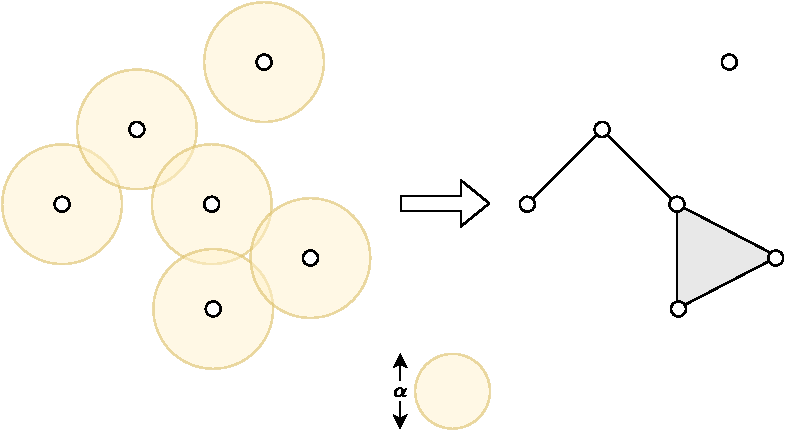
\includegraphics[width=0.7\textwidth]{thesis/figures/simplicial-complex-rips_cropped.pdf}
    \caption{Vietoris–Rips complex on 2-dimensional data with proximity diameter $\alpha$.}
    \label{fig:simplicial-complex-rips}
\end{figure}
By carefully studying the $n$-simplices of a Vietoris–Rips complex, we can observe topological structures such as \textit{loops} (i.e. $2$-simplices) or \textit{holes}  (i.e. $3$-simplices). We show an example of a loop in \cref{fig:simplicial-complex-rips}, where the rightmost data points that the bottom form a 2-simplex. In order to study topological properties of data, it is common to look at varying values of $\alpha$, starting at zero and increasing to infinity. In particular, we use what we call \textit{persistent homology}, which is the study of observing how the topology changes once a threshold (e.g. $\alpha$) increases. In order to easily present and visualize persistent homology, we use persistence diagrams. We look at persistence diagrams in the next subsection.

\subsection{Persistence diagram}
\label{sec:persistence diagram}
In order to present persistent homology of a simplicial complex, we use \textit{persistence diagrams}. Persistence diagrams we look at a range of proximity diameters over multiple persistent \textit{homology dimensions} (or \textit{homology degrees}), where the dimension refer to which $n$-simplices we want to look at (0-dimensional persistent homology observe changes of $0$-simplices, 1-dimensional observe changes of $1$-simplices, etc.). A persistence diagram is 2-dimensional, where the x-axis denotes the birth time and y-axis the death time. Assuming that we want to create a persistence diagram of data points, we let the proximity diameter $\alpha$ start at zero. By gradually increasing $\alpha$, new topological properties appear and old topological properties merge into other properties. In particular, once a topological property is "birthed" (e.g. 1-simplex between two data points), the birth time is noted for the particular data point. A point in the persistence diagram appear once $n$-simplices merge into new $m$-simplices (e.g. three 1-simplex becoming a 2-simplex).

To motivate the use of persistence diagrams, we illustrate with a simple example in \cref{fig:persistence-diagram-example}, where we study the change of 0-dimensional persistent homology. In \cref{fig:persistence-diagram-example}, we see how the persistence diagram changes once we increase the proximity diameter $\alpha$, on a data set consisting of two blobs. In the first row (a), we let $\alpha=0.2$ and we observe that there are only two data points intersecting, thus leading to a single point in the persistence diagram. In the second row (b), we let $\alpha=1.5$ and we observe how the data points in each blob connect to each other, thus leading to several entries in the persistence diagram. For the last row (c), we let $\alpha=4.5$, and we observe that there is a single point and several points on the bottom in the persistence diagram. By looking at the plot on the left, we see how the two blobs intersect and all data points have connections to other data points with distance less or equal to $\alpha$. In addition to this, the last row (c) indicates that we have two clusters in our data, although our data is rather noisy and could be more compact.
\begin{figure}[H]
    \centering
    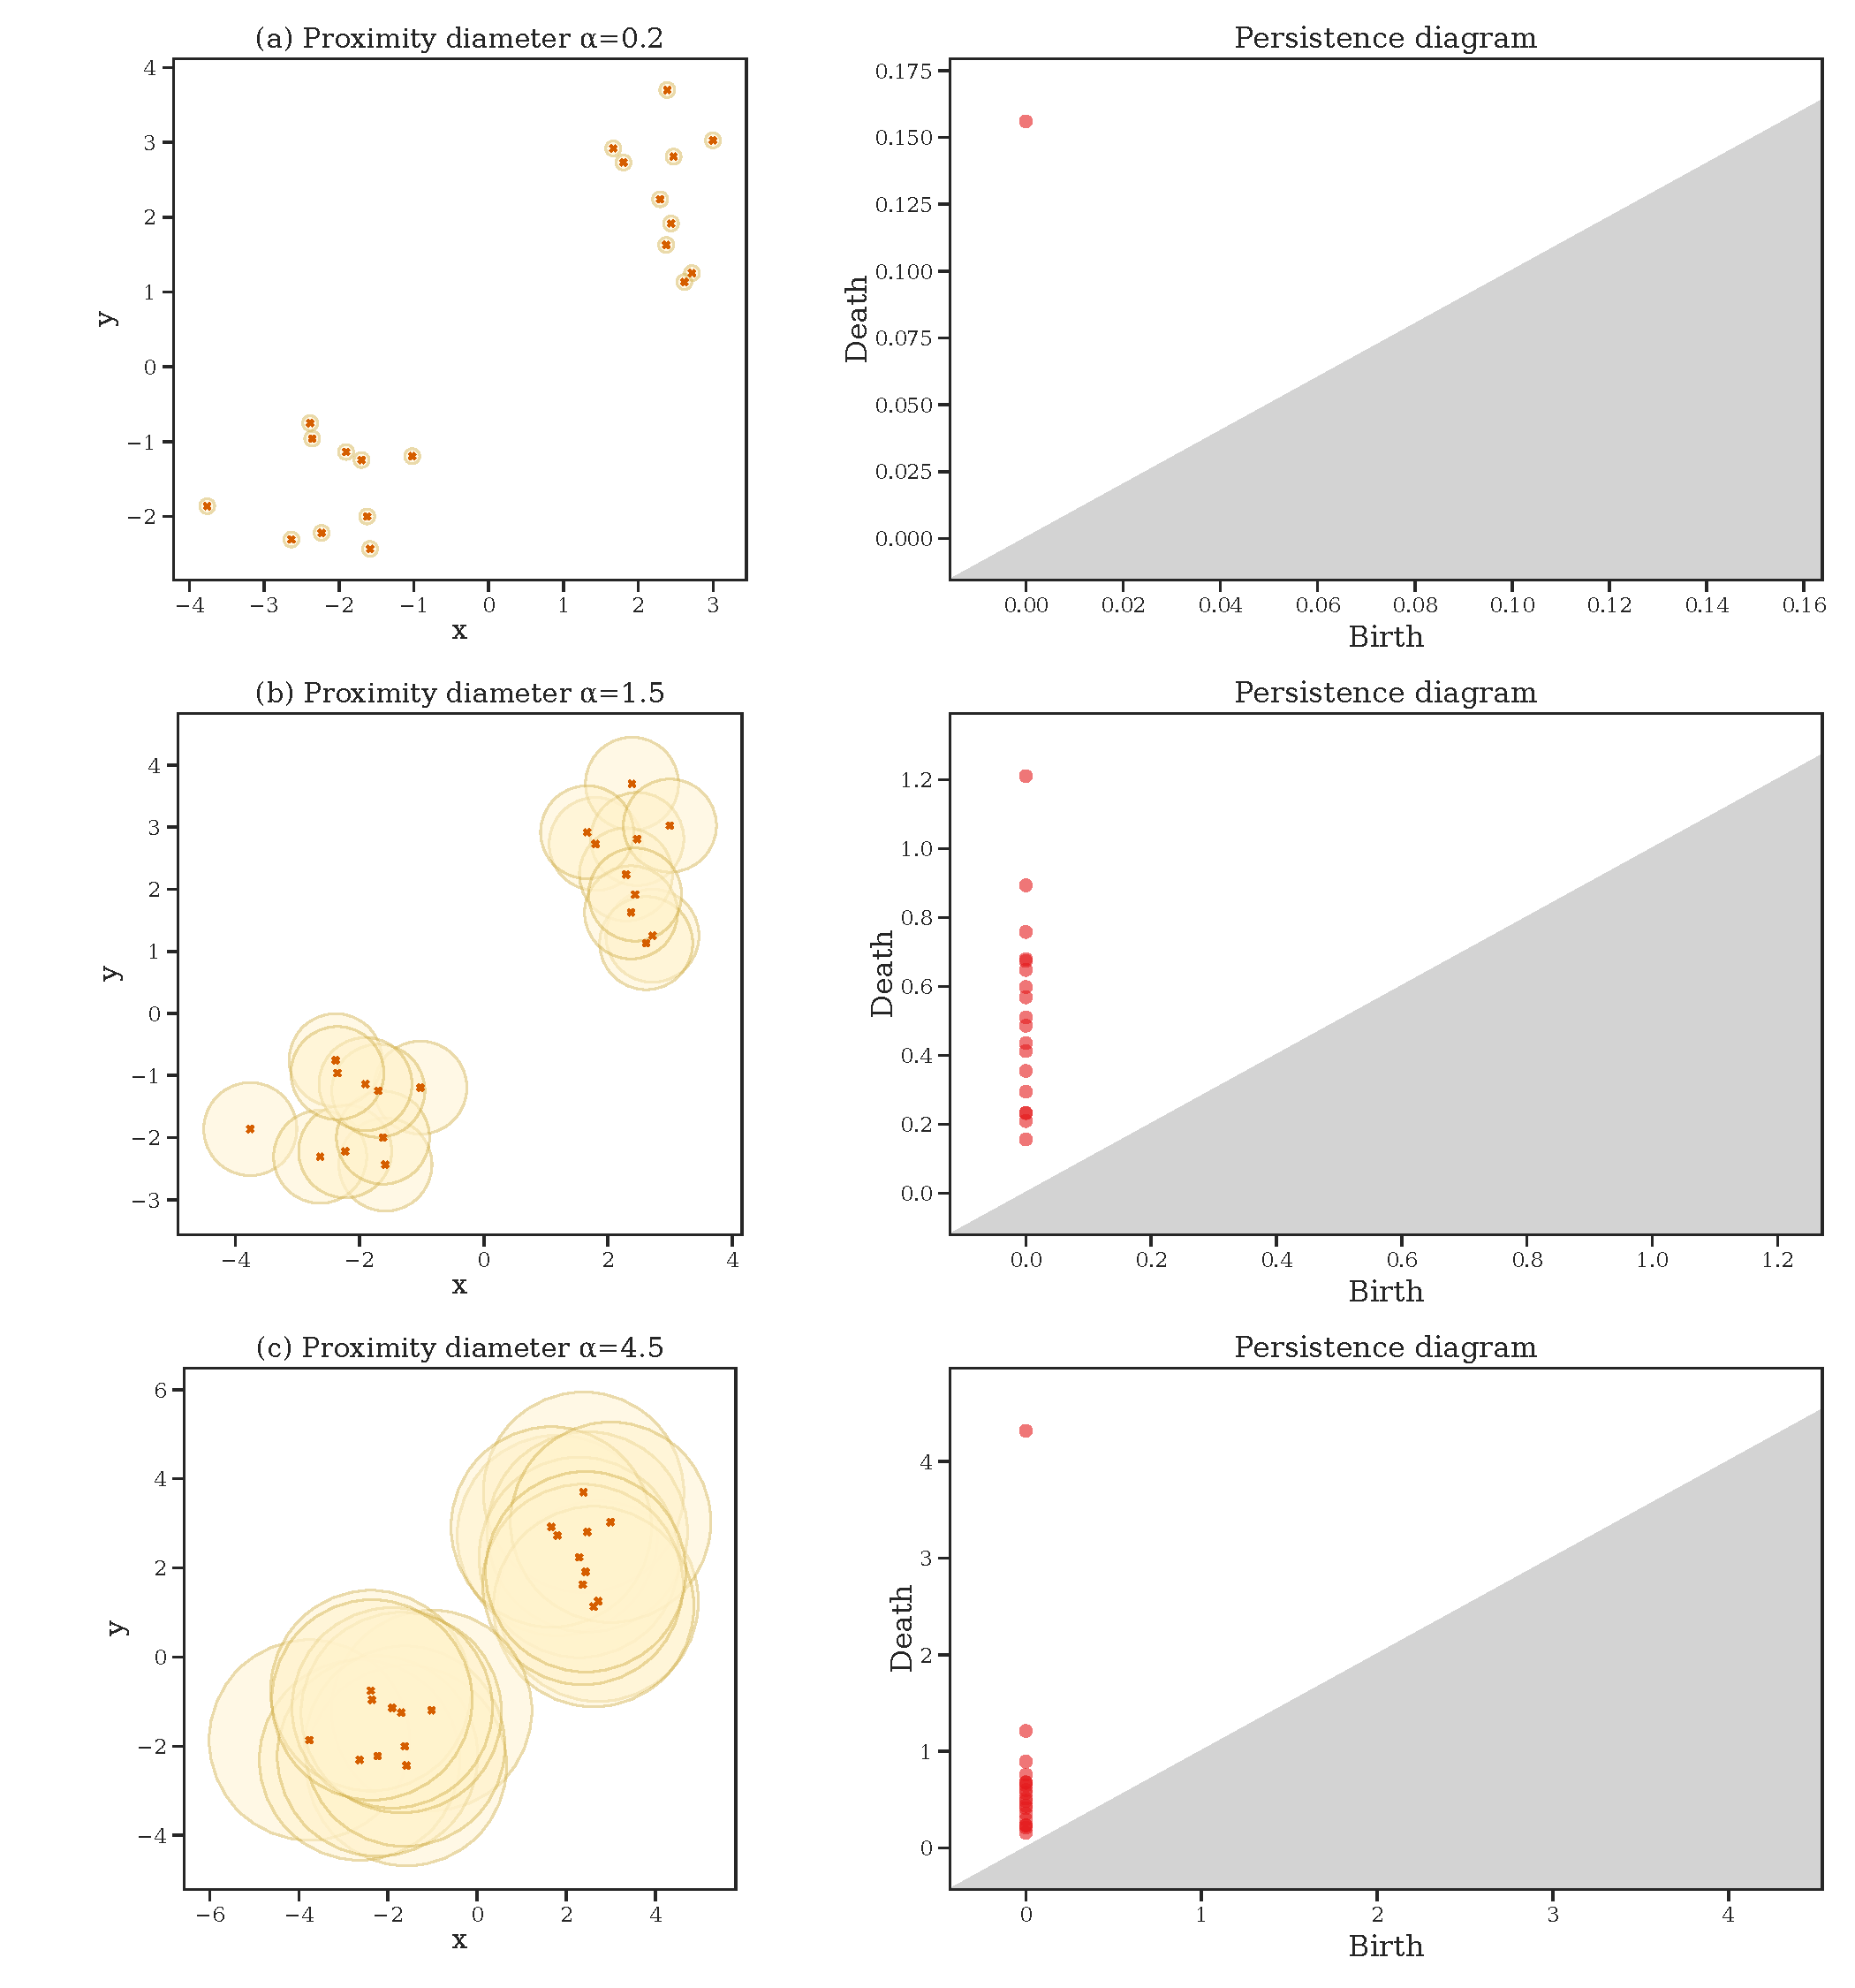
\includegraphics[width=1\textwidth]{thesis/figures/persistence-diagram-example.pdf}
    \caption{Persistence diagrams on different levels of $\alpha$ of a data set consisting of two blobs.}
    \label{fig:persistence-diagram-example}
\end{figure}
An important aspect of machine learning is to predict some quantity given some features. If we want to use the persistence diagrams as features in a model, for instance, a typical approach would be to perform some feature extraction or vectorization first. An example of a vectorization of persistence diagrams are persistence images, which we introduce in the next subsection.

\subsection{Persistence image}
\label{sec:persistence-image}
Many machine leaning tasks require valuable features in order to yield good results. \textit{Persistence images} \cite{adams2016persistence} are vector representations of persistence diagrams. When explaining persistence images, we refer to \cite{adams2016persistence}. Furthermore, we explain the use of persistence images in \cref{sec:analysis-of-embeddings-geometric-anomaly-detection} and when discussing future work in \cref{sec:future-work}.

Let $B = \enclc{\enclp{b_1, d_1}, \enclp{b_2, d_2}, \ldots, \enclp{b_m, d_m}} \in \R^{m \times 2}$ be a persistence diagram in birth-death coordinates. First, we transform $B$ into birth-persistence coordinates, where \textit{persistence} is the difference between death and birth. That is, let $T(B) = \enclc{\enclp{b_1, p_1}, \enclp{b_2, p_2}, \ldots, \enclp{b_m, p_m}} \in \R^{m \times 2}$, where $p_i = b_i - d_i$ for $1 \leq i \leq m$. Following, for each of the point in the the $T(B)$ persistence diagram, we place a probability distribution. A common choice is to use the Gaussian distribution, which we center at each data point respectively. By placing probability distributions on each point, we are able to differentiate between dense and sparse areas. In addition to placing probability distributions on each point, we weight the distributions by the persistence of the point, making more persistent areas more prominent than others. Using the weighted probability distributions, for a particular persistence diagram $B$ we define the persistence surface of $\rho_B$ as
\begin{align}
    \rho_B(z) = \sumlim{u \in T(B)}{} f(u) \phi_u(z),
\end{align}
where $f(u)$ is the persistence weighing function and $\phi_u(z)$ is the probability distribution which we evaluate at point $z$ (e.g. if Gaussian, then we center it at point $u$). Finally, we reduce the persistence surface $\rho_B(z)$ to a discretized representation. In particular, we form an $N \times M$ grid, and for each cell in the grid, we compute the integral of $\rho_B(z)$ over that region and use the result from the integral as value. In other words, this discretization allows us to summarize the persistence surface using less information and we are left with an $N \times M$ matrix which we can for machine learning tasks more easily.

\subsection{Wasserstein distance}
\label{sec:wasserstein-distance}
To compare distances between data points, we commonly use distance metrics (e.g. Euclidean distance). In order to compare differences between any two persistence diagrams $A$ and $B$, we use the $p$\textit{-Wasserstein distance}, which we define as
\begin{align}
    W_p(A, B) = \inf_{\gamma: A \rightarrow B} \enclp{\sumlim{u \in A}{} ||u - \gamma(u)||_{\infty}^{p}}^{1/p},
    \label{eqn:wasserstein-distance}
\end{align}
where $1 \leq p < \infty$ and $\gamma$ ranges over bijections between $A$ and $B$, and $\inf$ is the infimum (greatest lower bound, or similar to "minimum"). If we let $p=\infty$, i.e $W_\infty(A, B)$, we get what we call the \textit{bottleneck distance}. We use the bottleneck distance to compare persistence diagrams as well, but has the disadvantage of only using the maximum distance between any two points over the bijections between $A$ and $B$.

\subsection{Topological polysemy}
\label{sec:topological-polysemy}
Recall the manifold hypothesis, which states that, in general, real-life high-dimensional data tends to live on a low-dimensional sub-manifold embedded within the high-dimensional space \cite[p. 16]{bengio2014representation}. To give an example, imagine that we have gather some data about weight and height of humans. Naturally, we see that as the height increases, the weight increases as well. That is, we have a strong linear relationship (or correlation) between height and weight. We can therefore argue that the manifold dimension of the data is 1, even though the original data has dimension 2. The hypothesis should, in theory, also apply to word embeddings, but the authors of \cite{jakubowski2020topology} argue that word embeddings, should instead, live on a \textit{punched manifold}. By a pinched manifold, we mean a manifold where we "glue" together particular points that are equal in some sense, creating \textit{singular} areas in the manifold. We show an example of a pinched manifold in \cref{fig:pinched-manifold}, where we see an ideal pinched manifold for the word "solution" and four of its meanings as \textit{submanifolds}. For word embeddings, \cite{jakubowski2020topology} claim that these singular areas in the manifold represent polysemous words and that the neighbours of polysemous words share some relation to the polysemous word. In order to identify such polysemous words from word embeddings, \cite{jakubowski2020topology} introduce a topological measure of polysemy (using concepts from persistent homology) that correlates well with the true number of meanings of a word. To explain the topological measure of polysemy, we refer to \cite{jakubowski2020topology}.
\begin{figure}[H]
    \centering
    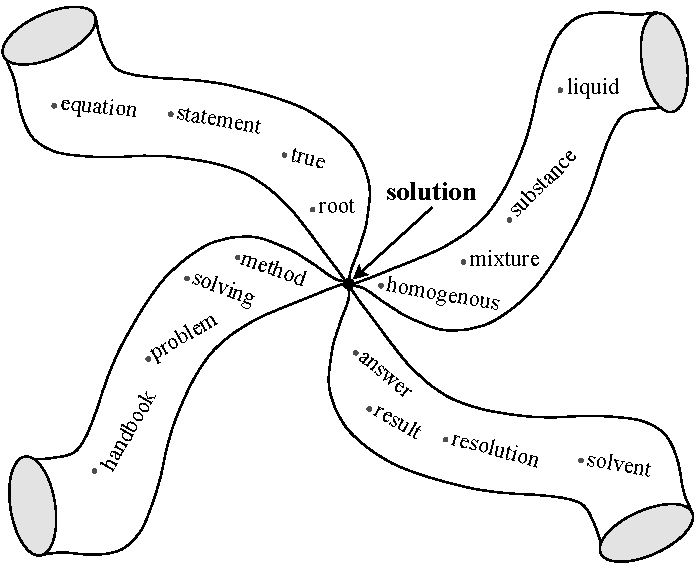
\includegraphics[width=0.7\textwidth]{thesis/figures/pinched-manifold_cropped.pdf}
    \caption{Pinched manifold of the word "solution", showing four of its meanings as submanifolds. This figure is inspired by \cite[Figure 5]{jakubowski2020topology}.}
    \label{fig:pinched-manifold}
\end{figure}

Determining the number of word meanings is a non-trivial task. Consider the word \textit{solution}, which has multiple meanings. In some contexts, the word \textit{solution} can relate to problem solving (e.g. solving a problem in a handbook), while in other contexts, it can be relate to chemistry (e.g. mixture of two or more substances). We call such words \textit{polysemous}, meaning that the word has multiple meanings which can relate to one another. The opposite of a polysemous word is a \textit{monosemous} word, meaning that the word only has one meaning. The motivation behind the topological measure of polysemy, as introduced by \cite{jakubowski2020topology}, stamps from the fact that the number of components of a \textit{punctured neighbourhood} around a word $w$ should reflect the number of word meanings of the word $w$. A punctured neighbourhood of $w$ are neighbouring words of $w$ excluding the word $w$ itself.

Let $W \in \R^{|V| \times d}$ be word embeddings, where $|V|$ is the number of words in the vocabulary and $d$ is the word embedding dimension. We compute the \textit{topological polysemy} $\text{TPS}_n(w)$ by fixing a target word $w$ and a neighbourhood size $n$. We denote the word vector of $w$ as $v_w \in \R^{d}$. To compute $\text{TPS}_n(w)$, we first normalize the word embeddings $W$ such that each vector are of unit length. We denote the normalized word embeddings as $W_\text{norm}$ and the normalized word vector of the target word $w$ as $v_{w_{\text{norm}}}$. Following, we compute the punctured neighbourhood $N_n(w)$, that is, the neighbouring $n$ normalized word vectors around $v_{w_{\text{norm}}}$, excluding $w$ itself. Furthermore, we project the word vectors of $N_n(w)$ to lie at the unit sphere, with $v_{w_{\text{norm}}}$ as the center. We denote this normalized punctured neighbourhood as $N'_n(w)$. In other words, we make the word vector of $w$ to be the origin of a $d$-dimensional sphere and project the neighbouring words of $w$ to lie around it. Lastly, we compute the 0-degree persistence diagram of $N'_n(w)$ and denote it as $PD_n(w)$. $\text{TPS}_n(w)$ is then the 1-Wasserstein distance (\cref{sec:wasserstein-distance}) between $PD_n(w)$ and the empty persistence diagram, also known as the Wasserstein norm. Furthermore, we use topological polysemy later when analysing word embeddings in \cref{sec:analysis-of-embeddings-topological-polysemy} and for prediction of polysemous words in \cref{sec:analysis-of-embeddings-supervised-polysemy-prediction}.

\subsection{Geometric Anomaly Detection}
\label{sec:geometric-anomaly-detection}
The manifold hypothesis forms a foundation of modern data science. Many manifold learning and dimensionality reduction algorithms rely on this assumption in order to find meaningful low-dimensional representations of high-dimensional data. Examples of such algorithms include PCA (\cref{sec:pca}) and UMAP (\cref{sec:umap}). \textit{Geometric Anomaly Detection} (GAD) \cite{stolz2020geometric} is an algorithm for identifying possible points in data which fail to satisfy the manifold hypothesis. Following, we describe the GAD algorithm and give a couple of examples of how it works. We refer to \cite{stolz2020geometric} when explaining the GAD algorithm.

To understand how the GAD algorithm works, we first introduce the motivation behind it. Imagine that we have some data that lies on two submanifolds $P$ and $Q$. We illustrate such a situation in \cref{fig:gad-motivation}. Here we assume that the two submanifolds $P$ and $Q$ are planes which intersect at some point, which we mark by the dotted red line. We place an \textit{annulus} around each data point and infer its topological structure. An annulus is the region between two circles, where the first circle is contained in the other, and both circles share center point. Annuli can also remind us of rings. Formally, each annulus around its respective data point has an inner radius $r$ and outer radius $s$. Depending on where a point is on either of the submanifolds, we observe that a point can have one of three states as seen in \cref{fig:gad-motivation}: (a), (b) or (c). If a point is at the boundary of either submanifolds, i.e. situation (a), we observe that the points falling into the annulus around the data point forms a half circle, as half of the circle does not have any data points in them. If we count the number of topological loops we get zero. If the data point falls nicely into either submanifold, i.e. situation (b), we observe that we get a nice annulus where neighbouring points falling into the annulus around the data point forms a circle. In other words, if a point is on the submanifold, we expect to get exactly one topological loop. For the last situation, i.e. (c), we have a data point which falls between $P$ and $Q$, creating a singularity (or anomaly) in the data. This stamps from the fact that it harder to distinguish which submanifold the particular data point should belong to. If we look at the data points in the annulus around the data point at situation (c), we observe that we get two or more topological loops.
\begin{figure}[H]
    \centering
    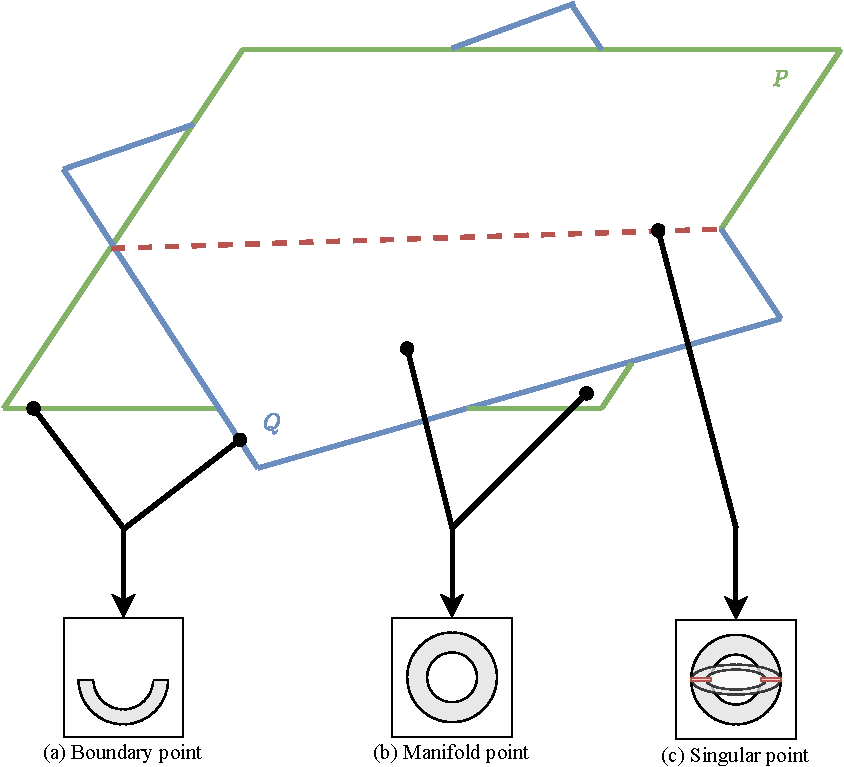
\includegraphics[width=0.8\textwidth]{thesis/figures/geometric-anomaly-detection-motivation_cropped.pdf}
    \caption{Motivation behind the GAD algorithm. Data points belonging to two submanifolds $P$ and $Q$, and depending on where the data points are on the submanifolds, it can have three different states: (a), (b) or (c). The GAD algorithm is particularity interested in finding singular (c) data points between $k$ submanifolds (here: $k=2$). This illustration is inspired by \cite[Figure 1]{stolz2020geometric}.}
    \label{fig:gad-motivation}
\end{figure}

Let $X \in R^{n \times d}$ be data points. The GAD algorithm works as follows: fix two parameters $0 < r < s$, and for each data point $x_i \in X$ place an annulus around it, with inner radius $r$ and outer radius $s$. Determine the data points that fall into the \textit{annular neighbourhood} of $x_i$ and denote this set as $A_y = \enclc{a_1, a_2, \ldots, a_m} \subset X$. That is, the set $A_y$ consists of those points $a_j$ that satisfies $r \leq d(x_i, g_j) \leq s$, where $d(\cdot, \cdot)$ measures the distance between two points (e.g. using Euclidean distance). Then, select a manifold dimension $k$ we would like to investigate, as the GAD algorithm discovers intersections of $(k-1)$ submanifolds. In order to find intersections of $(k-1)$ submanifolds of the annular neighbourhood $A_y$ of $x_i$, we compute the $(k-1)$-dimensional Vietoris–Rips complex of $A_y$, which we denote $VR_{k-1}(A_y)$. Then, for each birth-death coordinate $(b_{k-1}, d_{k-1}) \in VR_{k-1}(A_y)$, we count the number of points that persist longer as the annulus width. We denote this count as $N_y$. Recall that the persistence of points in persistence diagrams can be computed by transforming the persistence diagram into birth-persistence coordinates, where persistence $p_{k-1} = d_{k-1} - b_{k-1}$. We define the annulus width to be the difference between the outer and inner radius, i.e. $w_{A_y} = s - r$. To count $N_y$, we iterate over the points in the persistence diagram and count the number of points that satisfies
\begin{align}
    p_{k-1} > w_{A_y}.
    \label{eqn:gad-ny-condition}
\end{align}
The count $N_y$ is analogous to the number of topological loops that occur in $A_y$, for a particular homology dimension $(k-1)$. If no points satisfy \cref{eqn:gad-ny-condition}, i.e. $N_y=0$, then we classify $x_i$ as a boundary point, similar to the (a) situation in \cref{fig:gad-motivation}. If we have exactly one point that satisfies \cref{eqn:gad-ny-condition}, i.e $N_y=1$, then we classify the point as a boundary point, similar to the (b) situation in \cref{fig:gad-motivation}. If two or more points satisfy \cref{eqn:gad-ny-condition}, i.e. $N_y>1$, then we classify the point as a singular point, similar to the (c) situation in \cref{fig:gad-motivation}. Furthermore, we use GAD for later analysis of word embeddings in \cref{sec:analysis-of-embeddings-geometric-anomaly-detection} and for prediction of polysemous words in \cref{sec:analysis-of-embeddings-supervised-polysemy-prediction}. 
\chapter{Analysis of Word Embeddings}
\label{chap:analysis-of-word-embeddings}
In this chapter, we will use methods from machine learning to analyze word embeddings. Due to the scope of the thesis, we will mainly analyze word embeddings from the word2vec model (\cref{sec:word2vec}) using Skip-gram and negative sampling. We will also run some of the analysis methods on published word embeddings from external papers, in particular in \cref{sec:polysemous-words-prediction}.

Firstly, we will describe how we trained and evaluated our word2vec implementation. In particular, we will explain the data preprocessing steps, the implementation specifics and hyperparameter choices. We will also show how we evaluated our trained word2vec model. Secondly, we will perform cluster analysis on word embeddings to look for deeper structure. In particular, we will compare clustering algorithms trained on word embeddings, using internal cluster validation methods, and investigate the clustering of distinct groups of words. Thirdly, we will look at the application of two methods from topological data analysis on word embeddings. We end the chapter by creating two supervised models for estimating the number of word meanings, using the results from topological data analysis and intrinsic dimension estimation. We train the supervised models and visualize their evaluation results

To perform the analyses in this chapter, we utilized the Python programming language with some key Python packages: \path{numpy} \cite{2020NumPy-Array} (efficient vector and matrix manipulation), \path{scikit-learn} \cite{ScikitLearn2011} and \path{scipy} \cite{2020SciPy-NMeth} (general methods from machine learning), \path{matplotlib} \cite{Matplotlib2007} and \path{seaborn} \cite{seaborn2021} (tools for data visualization), \path{joblib} \cite{joblib2021} (data dumping to file), \path{sharedmem} \cite{sharedmem2020} (parallelization of trivial jobs) and \path{fastdist} \cite{fastdist2021} (fast distance calculations in Python). We ran the analysis code on a machine with two GPUs (GeForce RTX 2080 Ti $\times2$), one CPU (Intel i9-7900X @ 3.30GHz) and 64 GB of RAM. The computer was running an Ubuntu 18.04.5 operating system. In practice, we were only allotted to use a subset of the resources, as it was a shared computer by the research group in machine learning at the University of Bergen. Finally, the code used to perform the analyses is publicly available via GitHub in \cite{Triki2021}.

% Include sections
\section{Training and evaluation of word2vec}
\label{sec:training-and-eval-our-word2vec-impl}
In this section, we will describe how we trained and evaluated our word2vec model. In particular, we will explain the data preprocessing choices we made before training word2vec in \cref{sec:word2vec-data-preprocessing} and details of our implementation of word2vec using the Skip-gram model and negative sampling in \cref{sec:word2vec-impl-specifics}. Finally, we will cover the hyperparameter choices used to train the word2vec model in \cref{sec:word2vec-hyperparameter-choices} and evaluate the performance of the word2vec model using analogy test data sets in \cref{sec:word2vec-model-evaluation}.

\subsection{Data preprocessing}
\label{sec:word2vec-data-preprocessing}
To train a word2vec model, we require a sufficiently large data set (and thus embedding dimensionality) to yield good quality word embeddings \cite{mikolov2013b}. In the empirical experiments of \cite{mikolov2013b}, they used an internal data set based on data from Google News. Since this data set is not publicly available, we instead used dumps from \cite{WikimediaDumps} and performed several preprocessing steps, before training on it. In particular, we used the \textit{enwiki} (short for English Wikipedia) dump from 1st of January 2021 (20210101 on the Wikimedia pages). The dumps from Wikipedia were first downloaded and parsed using the WikiExtractor tool \cite{Wikiextractor2015}. Furthermore, we created a script using Python to merge and process output files from the WikiExtractor tool into a certain number of text files, such that we could train word2vec at ease. To benefit from parallel reading, we let the number of text files equal the number of CPU cores on our machine.

We then proceeded by processing each Wikipedia article. In particular, we performed the following steps:
\begin{enumerate}
    \item We split each article into a list of sentences using the \path{tokenize.sent_tokenize} function from the \path{nltk} Python package \cite{bird2009natural}.
    \item Then, we preprocessed each sentence individually.
    \begin{enumerate}
        \item We first replaced contractions in each sentence (e.g. I'll $\mapsto$ I will, you'd $\mapsto$ you would, etc.) by using the \path{contractions} Python package \cite{contractions-2016}.
        \item Then we split the sentence into a list of words using the \path{word_tokenize} function from \path{nltk}.
        \begin{enumerate}
            \item We replaced capital letters in words by the corresponding small letters (i.e. lower-case representation).
            \item We removed punctuation from words and create new sub-words for each word delimited by punctuation (e.g. out-of-the-box $\mapsto$ out, of, the, box).
            \item At last, we replaced all numbers (including ordinal numbers) with their textual representation, using the \path{num2words} Python package \cite{num2words2014}. For example, the number 10 was replaced by "ten", and the word "21st" was replaced by "twenty-first".
        \end{enumerate}
    \end{enumerate}
    \item With the new processed sentences, we filtered out sentences that had less than \textbf{min\_word\_count} words in them.
    \item Finally, we appended each sentence to an output text file, separated using the newline character (i.e. \textbackslash n).
\end{enumerate}

After processing the Wikipedia articles into files, we combined common phrases into single tokens. In particular, we followed the word2phrase procedure explained in \cref{sec:learning-word-embeddings-for-phrases}, resulting in tokens consisting of words separated by an underscore, e.g. the phrase "New York" becomes "new\_york". We denoted the threshold parameter from word2phrase as \textbf{threshold-word2phrase}. To create longer phrases of words, e.g. trigrams, four-grams or even five-grams, we repeated the word2phrase multiple times. In particular, we denote the number of repetitions as \textbf{num-epochs-word2phrase}, which we chose as a hyperparameter. Furthermore, for each repetition of word2phrase, the threshold parameter $\delta$ is decreased. \cite{mikolov2013b} did not state how they decreased this parameter, however, but by inspection of the source code of word2vec \cite{Word2vecDemoPhrasesCode}, we observed that they started with a threshold of 200, then decreased it to 100 for the second and final repetition. With this in mind, we introduce a threshold decay hyperparameter, denoted \textbf{threshold-decay-word2phrase}, which tells how much the threshold decreases for each repetition of word2phrase.

\subsection{Implementation specifics}
\label{sec:word2vec-impl-specifics}
To implement the word2vec model, we used Python and TensorFlow \cite{tensorflow2015-whitepaper}. In addition to this, we used the \path{numpy} \cite{2020NumPy-Array} package to work with vectors and matrices more easily. In particular, we implemented the Skip-gram model using negative sampling. To do so, we split our implementation into three main Python classes. The first class is the \path{Tokenizer} class, which is responsible for converting text into word indices in vocabulary (e.g. the word "hello" $\mapsto$ 42). The second class is the \path{Word2vecSGNSModel}, which inherits the \path{tf.keras.Model} class from TensorFlow; we created the model via subclassing, as specified in \cite{TensorflowSubclassing2020}. \path{Word2vecSGNSModel} is the model we used to train our ANN. The third and final main class is \path{Word2vec}. It performs training using the \path{Word2vecSGNSModel} and uses \path{Tokenizer} to convert words into integers.

To load the data into the model, we used the \path{tf.data} API, as introduced in TensorFlow 2. The \path{tf.data} API allows us to create flexible and scalable data generators. As mentioned in \cref{sec:word2vec-data-preprocessing}, we want to train our model on dumps from Wikipedia, i.e., several gigabytes of raw text data, and the \path{tf.data} API allows us to exactly this quickly and efficiently. In particular, we used the \path{tf.data.TextLineDataset} class to load multiple text files in parallel and set \path{num_parallel_calls} to \path{tf.data.experimental.AUTOTUNE} wherever we could, such that we parallelize the data generation process as much as possible. We also used \path{prefetch} to prepare the data in parallel while training.

We implemented word2phrase using Python. First, we counted the uni- and bigram word occurrences, and using them, we ran the word2phrase procedure as explained in \cref{sec:learning-word-embeddings-for-phrases} by accepting bigrams into the vocabulary if the score (from \cref{eqn:word2phrase-score}) is greater than the set threshold parameter.

By implementing word2vec ourselves, we learned a few things we did not realize after reading the two papers from Mikolov et al. \cite{mikolov2013a, mikolov2013b}:
\begin{itemize}
    \item Training on big data sets (e.g. dumps from Wikipedia) requires an efficient implementation of the data generator. We first attempted to create a data generator that loaded everything into memory, but it became clear to us that this did not scale well when we later wanted to train on bigger data sets.
    \item The preprocessing of data may drastically change the quality of the word embeddings.
    \item That we have two embedding matrices $W$ and $W'$ corresponding to the input and output of the network. At first, we only had a single embedding matrix, for both the input and the output of the network.
\end{itemize}

\subsection{Hyperparameter choices}
\label{sec:word2vec-hyperparameter-choices}
To train the word2vec model, we based our choices of hyperparameters on the different choices used in models from \cite{mikolov2013a, mikolov2013b}. These hyperparameters can be found in \cref{table:word2vec-hyperparameter-choices}.

\begin{table}[ht]
    \centering
    \begin{tabular}{@{}ll@{}}
    \toprule
    Hyperparameter & Value\\
    \midrule
    \trcolor \textbf{min-word-count} & 5\\
    \textbf{max-vocab-size} & $\infty$ \\
    \trcolor \textbf{batch-size} & 256\\
    \textbf{num-epochs} & 5\\
    \trcolor \textbf{num-epochs-word2phrase} & 2\\
    \textbf{threshold-word2phrase} & 200\\
    \trcolor \textbf{threshold-decay-word2phrase} & 0.5\\
    \textbf{learning-rate} & 0.025\\
    \trcolor \textbf{min-learning-rate} & 0.0000025\\
    \textbf{embedding-dim} & 300\\
    \trcolor \textbf{max-window-size} & 5\\
    \textbf{num-negative-samples} & 5\\
    \trcolor \textbf{sampling-factor} & 0.00001\\
    \textbf{unigram-exponent} & 0.75\\
    \bottomrule
    \end{tabular}
    \caption{Hyperparameters used to train our word2vec model}
    \label{table:word2vec-hyperparameter-choices}
\end{table}

Similar to \cite{mikolov2013b}, we set the minimum word count to 5 and did not restrict the maximum vocabulary size. In other words, we let the vocabulary include words that occur at least 5 times in the training data.

We set the number of repetitions for word2phrase to 2 and the initial threshold to 200, as \cite{mikolov2013b} did in their experiments. Furthermore, we set the threshold decay to 0.5 (i.e. the threshold is halved for each repetition) to use a similar setup.

Neither \cite{mikolov2013a} nor \cite{mikolov2013b} stated which batch-size they used, but by inspecting the source code \cite[line 542]{Word2vecCCode}, we concluded that they used 1 as their batch size, i.e., performing a backward pass for every forward pass in the model. We found, however, that setting the batch size to 256 to be a nice fit for our data, leading to good quality vectors and faster training.

Mikolov et al. used 1 to 4 epochs in their experiments \cite{mikolov2013a, mikolov2013b}, and in the source code of word2vec \cite[line 43]{Word2vecCCode}, they default to 5 epochs. For this reason, we set the number of epochs to 5.

We set the initial and minimum learning rate to 0.025 and 0.000025, respectively, as noted in \cite{mikolov2013a} and the source code of word2vec \cite[lines 44 and 398]{Word2vecCCode}.

Furthermore, we set the embedding dimension to 300, the maximal window size to 5, the number of negative samples to 5, the sampling factor to 0.00001 and the unigram exponent to 0.75, similar to experiments from \cite{mikolov2013b}.

Using the preprocessing steps from \cref{sec:word2vec-data-preprocessing} on our data and the hyperparameters from \cref{table:word2vec-hyperparameter-choices}, we get a vocabulary size of $\sim$4.4 million words and corpus size (i.e number of words used from the \textit{enwiki} data set) of $\sim$2.3 billion words.

\subsection{Model evaluation}
\label{sec:word2vec-model-evaluation}
We trained the word2vec model using data preprocessing steps from \cref{sec:word2vec-data-preprocessing} and hyperparameters from \cref{sec:word2vec-hyperparameter-choices}. Following, we will refer to our trained word2vec model as \textit{SGNS-enwiki} (short for \textbf{S}kip-\textbf{g}ram \textbf{n}egative \textbf{s}ampling-enwiki). To show that the trained word embeddings from the SGNS-enwiki model can be used for word analogy tasks, we evaluated the SGNS-enwiki model using analogy test data sets. The goal of performing these tests is to show that the word embeddings of SGNS-enwiki are comparable to word embeddings from other published (pre-trained) models, in terms of quality.

In particular, we used three analogy test data sets, namely the \textit{Semantic-Syntactic Word Relationship test set} (SSWR), the \textit{Microsoft Research Syntactic Analogies Dataset} (MSR) and the \textit{Phrase Analogy Dataset} (PAD). The SSWR test data set was first introduced in \cite{mikolov2013a}, consists of 8869 semantic and 10675 syntactic questions and is widely used as a test data set. The MSR data set was first introduced in \cite{mikolov-etal-2013-linguistic} and consists of 8000 analogy questions. To evaluate word embedding models trained on phrases (e.g. "New York Times"), \cite{mikolov2013b} introduced the PAD. PAD consists of 3218 analogy questions. It should be noted, however, that there are other common test data sets as well, such as the Bigger analogy test set (BATS) from \cite{gladkova-etal-2016-analogy}.

We compared the results from the evaluation of our word2vec model to models from \cite{mikolov2013a, mikolov2013b, mikolov-etal-2013-linguistic, bojanowski2017enriching}. In particular, we compared to the Skip-gram models from \cite[Table 3]{mikolov2013a} and \cite[Table 6]{mikolov2013a} (denoted \textit{SG 300} and \textit{SG 1000} respectively), the \textit{NEG-15} model from \cite[Table 1 and 3]{mikolov2013b}, the \textit{RNN-1600} model from \cite[Table 2]{mikolov-etal-2013-linguistic} and the \textit{fastText} model from \cite[Table 2]{bojanowski2017enriching}.

The results are shown in \cref{table:word2vec-eval-sswr,table:word2vec-eval-msr,table:word2vec-eval-pad}. A dash (--) denotes that the model has not been evaluated on the particular subset/data set, and \textbf{bold} values indicate the best value. Values represent accuracies and are in percentages.
\begin{table}[H]
    \centering
    \begin{tabular}{@{}cccc@{}}
    \toprule
    & \multicolumn{3}{c}{SSWR} \\ \cmidrule(l){2-4}
    \multirow{-2}{*}{Model} & Semantic & Syntactic & Average \\ \midrule
    \trcolor
    SG 300 & 55 & 59 & 57 \\
    SG 1000 & 66.1 & 65.1 & 65.6 \\
    \trcolor
    NEG-15 & 61 & 61 & 61 \\
    RNN-1600 & -- & -- & -- \\
    \trcolor
    fastText & \textbf{77.8} & \textbf{74.9} & \textbf{76} \\
    SGNS-enwiki & 65.8 & 67.3 & 66.6 \\
    \bottomrule
    \end{tabular}
    \caption{Comparison of empirical results using the SSWR word analogy test data set.}
    \label{table:word2vec-eval-sswr}
\end{table}
\begin{table}[H]
     \centering
    \begin{tabular}{@{}ccccc@{}}
    \toprule
    & \multicolumn{4}{c}{MSR} \\
    \cmidrule(l){2-5} 
    \multirow{-2}{*}{Model} & Adjectives & Nouns & Verbs & Average \\
    \midrule
    \trcolor
    SG 300 & -- & -- & -- & \textbf{56} \\
    SG 1000 & -- & -- & -- & -- \\
    \trcolor
    NEG-15 & -- & -- & -- & -- \\
    RNN-1600 & 23.9 & 29.2 & \textbf{62.2} & 39.6 \\
    \trcolor
    fastText & -- & -- & -- & -- \\
    SGNS-enwiki & \textbf{43.1} & \textbf{62.5} & 59.1 & 54.9 \\
    \bottomrule
    \end{tabular}
    \caption{Comparison of empirical results using the MSR word analogy test data set.}
    \label{table:word2vec-eval-msr}
\end{table}
\begin{table}[H]
    \centering
    \begin{tabular}{@{}cc@{}}
    \toprule
    & PAD \\
    \cmidrule(l){2-2}
    \multirow{-2}{*}{Model} & Average \\
    \midrule
    \trcolor
    SG 300 & -- \\
    SG 1000 & -- \\
    \trcolor
    NEG-15 & 42 \\
    RNN-1600 & -- \\
    \trcolor
    fastText & -- \\
    SGNS-enwiki & \textbf{53.7} \\
    \bottomrule
    \end{tabular}
    \caption{Comparison of empirical results using the PAD word analogy test data set.}
    \label{table:word2vec-eval-pad}
\end{table}

From \cref{table:word2vec-eval-sswr}, we see that our word2vec model is fairly competitive in terms of accuracy on the SSWR analogy test data set. The fastText model, however, is the most accurate model on this test data set, being approximately 10\% more accurate, on average. The same story goes for the results from the MSR test data set, as seen in \cref{table:word2vec-eval-msr}, where SGNS-enwiki performs pretty well, falling short for the SG 300 on average. Lastly, from \cref{table:word2vec-eval-pad} we see that SGNS-enwiki outperforms the NEG-15 model. We note that we had a lot of missing data for this evaluation, as all models had not been evaluated for every (subset of the) test data set. This evaluation, however, indicates that SGNS-enwiki understands syntactic and semantic relationships between words.

To gain further insight into how the vector representations learned by SGNS-enwiki are, we inspected the nearest neighbours of words. In \cref{table:word2vec-nearest-neighbours-words} we show a sample of such comparison, using the 5 nearest neighbouring words (also some phrases) for each query word. We used cosine similarity to find the neighbouring words, excluding the query word from the search.
\begin{table}[H]
    \centering
    \begin{tabular}{@{}ll@{}}
    \toprule
    Query word & Neighbouring words \\ \midrule
    \trcolor
    Apple        & Apple Inc., Blackberry, Apple computer, OneScanner, released Xsan \\
    Phone      & Phones, mobile phone, cell phone, cellphone, phone calls \\
    \trcolor
    Water   & Fresh water, drinking water, water pumped, salinated, untreated water \\
    Sunny      & Windy, dry sunny, warm sunny, cool, Lee Hany Lee \\
    \trcolor
    Book      & Books, book entitled, Tarcher Penguin, author, foreword \\ \bottomrule
    \end{tabular}
    \caption{Nearest 5 neighbouring words for some query words, using our word2vec model.}
    \label{table:word2vec-nearest-neighbours-words}
\end{table}
From \cref{table:word2vec-nearest-neighbours-words}, we see the ability of SGNS-enwiki to identify related words to the query word.

We visualize the ability of SGNS-enwiki to identify underlying concepts of the language and relationships between them in \cref{fig:sgns-enwiki-word-to-word-relations-pca-2d}, using a 2-dimensional PCA (\cref{sec:id-estimation-lpca}) embedding of words representing countries/capitals and comparative adjectives (e.g. good $\rightarrow$ better $\rightarrow$ best). From \cref{fig:sgns-enwiki-word-to-word-relations-pca-2d}, we observe the ability of the SGNS-enwiki model to learn underlying concepts, such as what capital means and how comparative adjectives behave. In addition to this, we also observe some clustering occurring in both plots. In particular, we observe that Scandinavian countries and capitals are more clustered to the top of \cref{fig:sgns-enwiki-word-to-word-relations-pca-2d} (a), and words related to temperatures are more clustered to the right of \cref{fig:sgns-enwiki-word-to-word-relations-pca-2d} (b).
\begin{figure}[H]
   \centering
   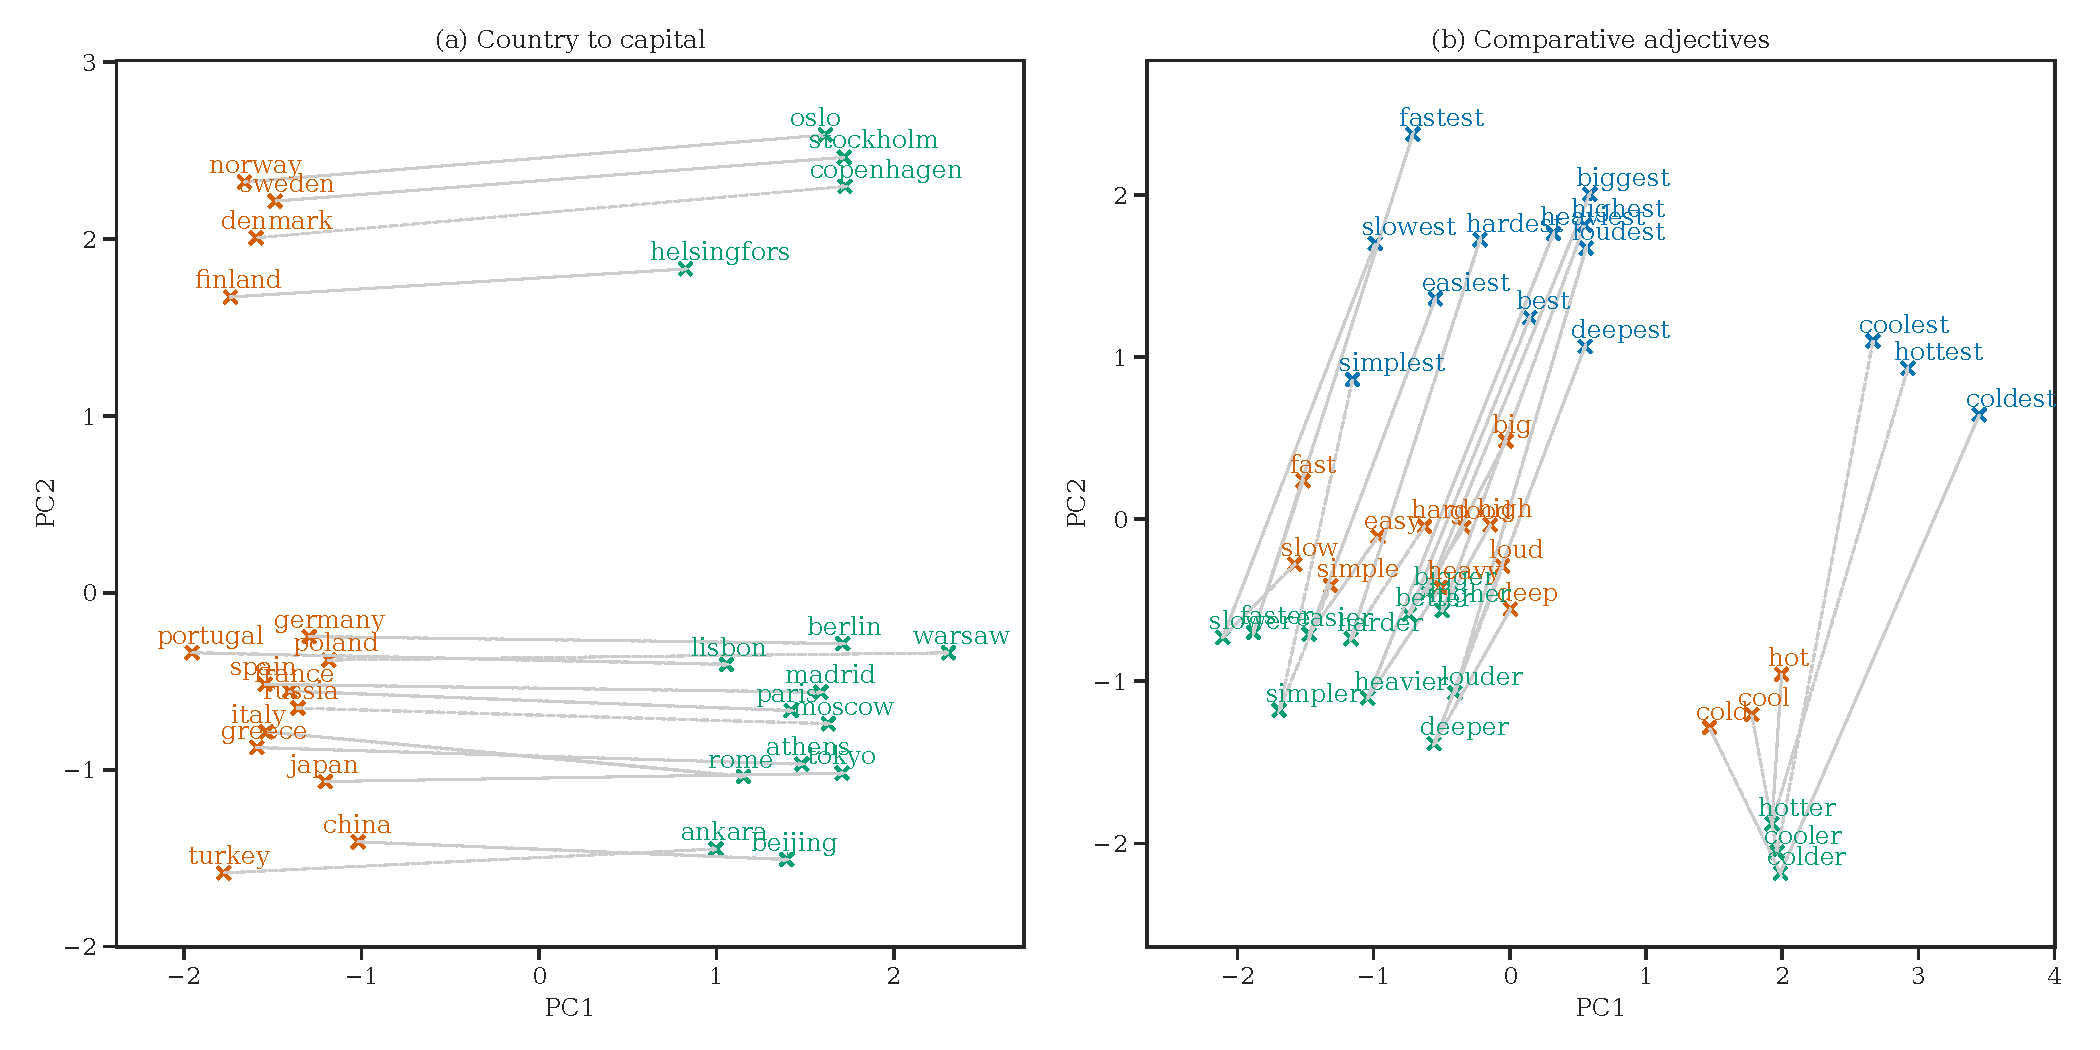
\includegraphics[width=\textwidth]{thesis/figures/word-to-word-relationships-pca-2d.pdf}
 \caption{2-dimensional PCA projection of the word embeddings of SGNS-enwiki of some countries and their capital cities (a) and comparative adjectives (b). This figure is inspired by \cite[Figure 2]{mikolov2013b}.}
 \label{fig:sgns-enwiki-word-to-word-relations-pca-2d}
\end{figure}

Due to the apparent clustering occurring in both plots from \cref{fig:sgns-enwiki-word-to-word-relations-pca-2d}, we will investigate the notion of clustering further. To deepen our understanding of the underlying structure of the SGNS-model, we will in the next section perform cluster analysis of its word embeddings. In particular, we will use multiple clustering algorithms and internal cluster validation methods to find the most suitable clustering algorithm and the number of clusters.
\section{Word clustering}
\label{sec:analysis-of-word-embeddings-word-clustering}
In this section, we will apply cluster analysis on the word embeddings of the SGNS-enwiki, in order to search for deeper structures within the data. In particular, we will compare clustering algorithms on the word embeddings of the SGNS-enwiki in \cref{sec:comparing-clustering-algorithms}, and following, we will look at clustering of distinct groups of words in \cref{sec:clustering-word-groups}.

\subsection{Comparing clustering algorithms}
\label{sec:comparing-clustering-algorithms}
In this subsection, we compare clustering algorithms on the word embeddings of the SGNS-enwiki. Due to the large number of words in the vocabulary of the SGNS-enwiki (roughly 4.4 million, see \cref{sec:word2vec-hyperparameter-choices} for more details), we restrict the analysis to the 10000 most common (i.e most frequently occurring) words. This way, we speed up the computation by reducing the computational requirement, but should still get a reasonable result, as the most common words yield good quality vector representations (more data $\rightarrow$ better vectors).

To perform the cluster analysis, we use all clustering algorithm from \cref{sec:clustering-algorithms}, except for Spectral clustering (\cref{sec:spectral-clustering}), as it was too computationally expensive for it to run. In particular, we used the following algorithms: k-means clustering (\cref{sec:k-means-clustering}), mini-batch k-means clustering (\cref{sec:mini-batch-k-means-clustering}), k-medoids clustering (\cref{sec:k-medoids-clustering}), GMMs (\cref{sec:gmm-clustering}), hierarchical clustering (agglomerative) (\cref{sec:hierarchical-clustering}), HDBSCAN (\cref{sec:hdbscan-clustering}) and ToMaTo (\cref{sec:tomato-clustering}). We used the \path{scikit-learn} \cite{ScikitLearn2011} and \path{hdbscan} \cite{mcinnes2017hdbscan} Python packages to perform clustering. Furthermore, we trained each of the clustering algorithms using a grid-search manner, i.e. by trying all combinations of hyperparameters. \cref{table:hyperparameters-clustering-algorithms} shows the hyperparameters used to train each clustering algorithm. By forming a grid of hyperparameters for each clustering algorithm, we get a rough sense for the best set of hyperparameters. For the initial grid-search, we used the same number of clusters for all the algorithms that allows us to specify the number of clusters. Let \path{n_clusters_range}=2, 3, 4, 5, 10, 50, 100, 150, 200, 300, 400, 500, 750, 1000, 1500, 2000, 3000, 4000, 5000, 6000, 7000, 8000 be the range of cluster numbers used for the initial grid-search. We let \path{n_clusters_range} range from 2 to 8000 clusters, using varying step sizes, to investigate the effect of the number of clusters for each algorithm, where it was applicable. To train the clustering algorithm, we use the standard word embeddings if the algorithm supports cosine similarity (or distance) and normalized word embeddings if the algorithm requires Euclidean distances. After training the clustering algorithms, we validated them using the internal cluster validation methods from \cref{sec:cluster-validation}. In particular, we used the mean Silhouette Coefficient (SC)) (\cref{sec:silhouette-coefficient}), the Davies-Bouldin Index (DBI) (\cref{sec:davies-bouldin-index}) and the Caliński-Harabasz Index (CHI) (\cref{sec:calinski-harabasz-index}). We used the \path{scikit-learn} Python package to perform internal clustering validation.
\begin{table}[H]
    \centering
    \begin{tabular}{@{}lll@{}}
    \toprule
    Clustering algorithm                           & Hyperparameters & Values \\
    \midrule
    \trcolor K-means clustering & \path{n_clusters} & \path{n_clusters_range} \\
    \multirow{2}{*}{Mini-batch k-means clustering} & \path{n_clusters} & \path{n_clusters_range} \\
                                                   & \path{batch_size} & 100 \\
    \trcolor K-medoids clustering & \path{n_clusters} & \path{n_clusters_range} \\
    GMM clustering & \path{n_components} & \path{n_clusters_range} \\
    \trcolor & \path{n_clusters} & \path{n_clusters_range} \\
    \trcolor \multirow{-2}{*}{Agglomerative clustering} & \path{linkage} & \path{single}, \path{average}, \path{complete}, \path{ward} \\
    \multirow{2}{*}{HDBSCAN} & \path{min_cluster_size} & 2, 4, 8, 16, 32, 64 \\
                             & \path{min_samples} & 1, 2, 4, 8, 16, 32, 64\\
    \trcolor                         & \path{density_type} & \path{DTM}, \path{logDTM}, \path{KDE}, \path{logKDE} \\
    \trcolor \multirow{-2}{*}{ToMATo} & \path{k} & 2, 3, \ldots, 10, 20, \ldots, 50, 100, \ldots, 250 \\
    \bottomrule
    \end{tabular}
    \caption{Hyperparameters of clustering algorithms for cluster analysis.}
    \label{table:hyperparameters-clustering-algorithms}
\end{table}

We visualize the result from the initial grid-search in \cref{fig:cluster-analysis-comparison-internal-cluster-validation}. From \cref{fig:cluster-analysis-comparison-internal-cluster-validation}, we see that agglomerative clustering algorithm performs the best (close to k-means clustering) and k-medoids clustering  performs the worst. For this reason, we will now focus on the agglomerative clustering algorithm and search for the best set of hyperparameters, being the linkage criterion and number of clusters.
\begin{figure}[H]
    \centering
    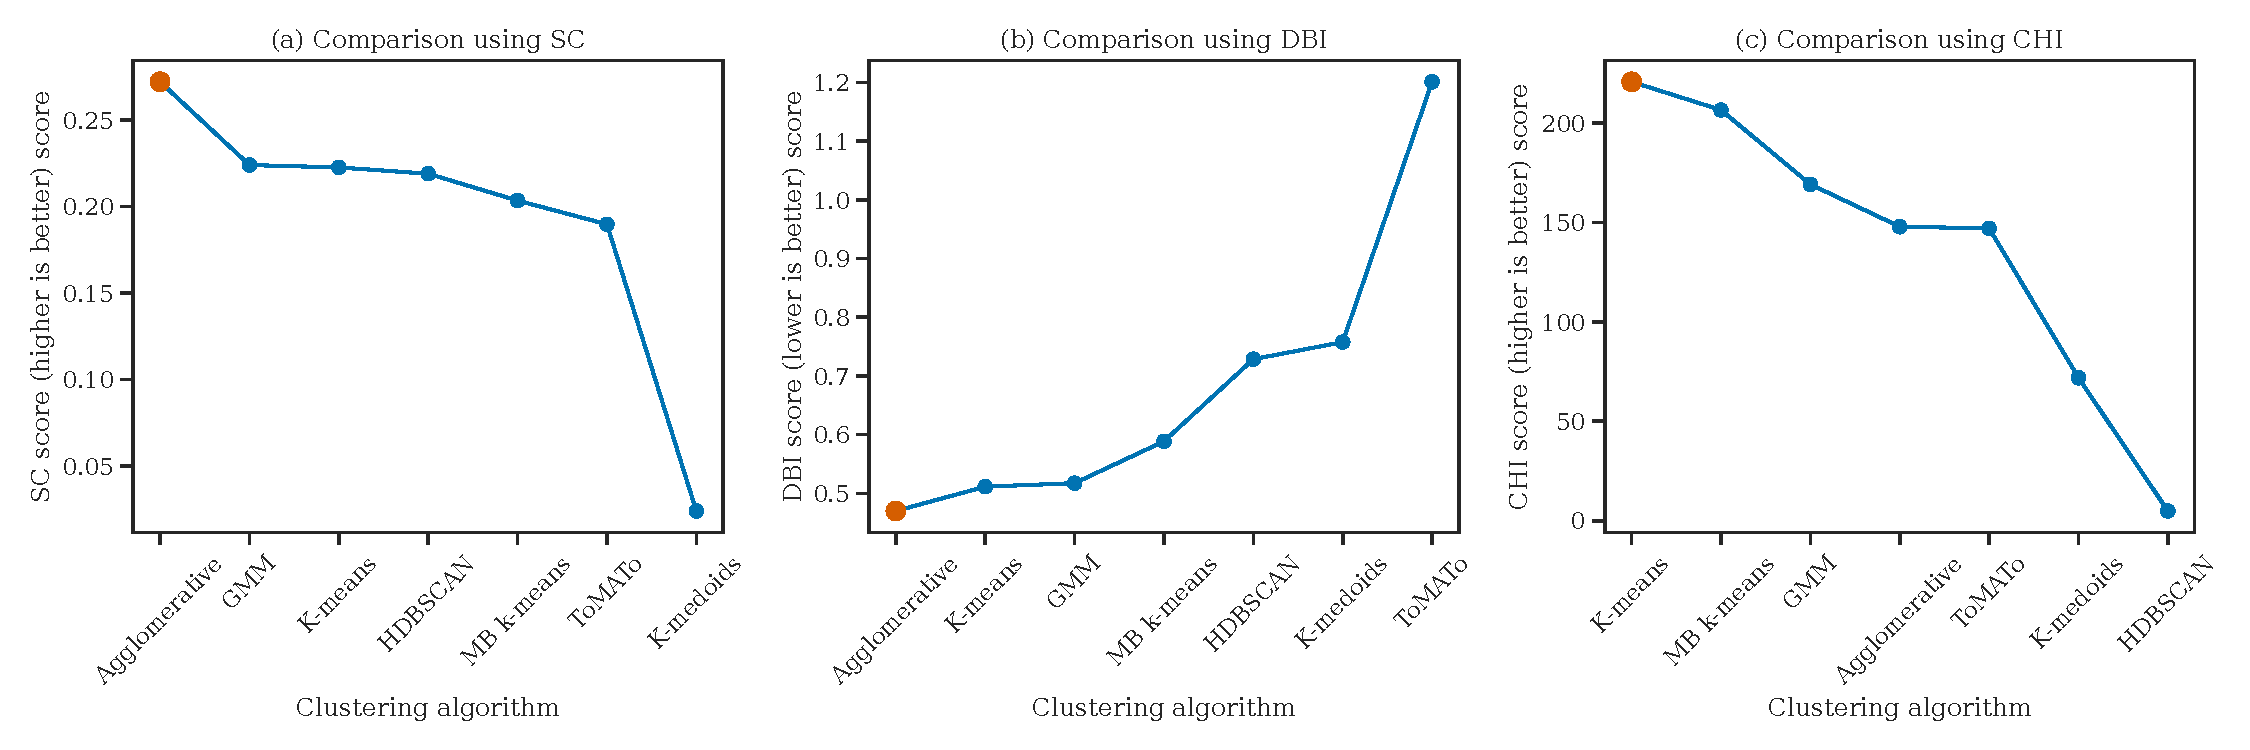
\includegraphics[width=\textwidth]{thesis/figures/cluster-analysis-comparison-internal-cluster-validation.pdf}
    \caption{Comparison of clustering algorithms trained on word embeddings from SGNS-enwiki, ranked by internal cluster validation methods. The red dot in each plot denotes the most optimal value.}
    \label{fig:cluster-analysis-comparison-internal-cluster-validation}
\end{figure}

In order to find the best set of hyperparameters using the agglomerative clustering algorithm, we first visualize its results from the initial grid search in \cref{fig:cluster-analysis-agglomerative-internal-cluster-validation}. From \cref{fig:cluster-analysis-agglomerative-internal-cluster-validation}, first notice that by using the single linkage criterion, we get relatively poor results. The remaining criterions, average, complete and ward, perform more or less the same over all internal clustering validation methods, with the ward criterion being slightly ahead of the rest. By inspecting the best value for the number of clusters for each internal cluster validation method in \cref{fig:cluster-analysis-agglomerative-internal-cluster-validation}, we noticed that the DBI (b) and the CHI (c) gave misleading results, while the SC (a) were more meaningful. In particular, the DBI prefers to have the largest number of clusters, that is, 8000 clusters. We inspected the clusters and observed that 6350 of the words are in its own cluster of size 1. This means that the DBI is not particularly well suited for choosing the number of clusters, as it prefers to have the most clusters. This is also illustrated by looking at the plot in the middle (b) of \cref{fig:cluster-analysis-agglomerative-internal-cluster-validation}. Using the CHI, we observe that it prefers to have the least number of clusters, namely 2. We inspected this result, and noticed that in the first clusters, there were only a single word, while the second cluster had the remaining 9999 words. In other words, this means that the CHI is also not particularly well suited for choosing the number of clusters. Finally, using the SC (a), we observe that the preferred number of clusters lie around 3000 to 6000. We inspected the number of clusters as preferred by average, complete and ward linkage clustering and concluded that they made sense, as there were more variety in the cluster sizes and the number of clusters having the specific each cluster sizes. This indicates that the most preferable number of clusters (using SC) should lie in this range (3000 to 6000), and following, we will narrow down the search for the best number of clusters. For the next experiment, we will not include the single linkage clustering criterion, as it performed poorly.
\begin{figure}[H]
    \centering
    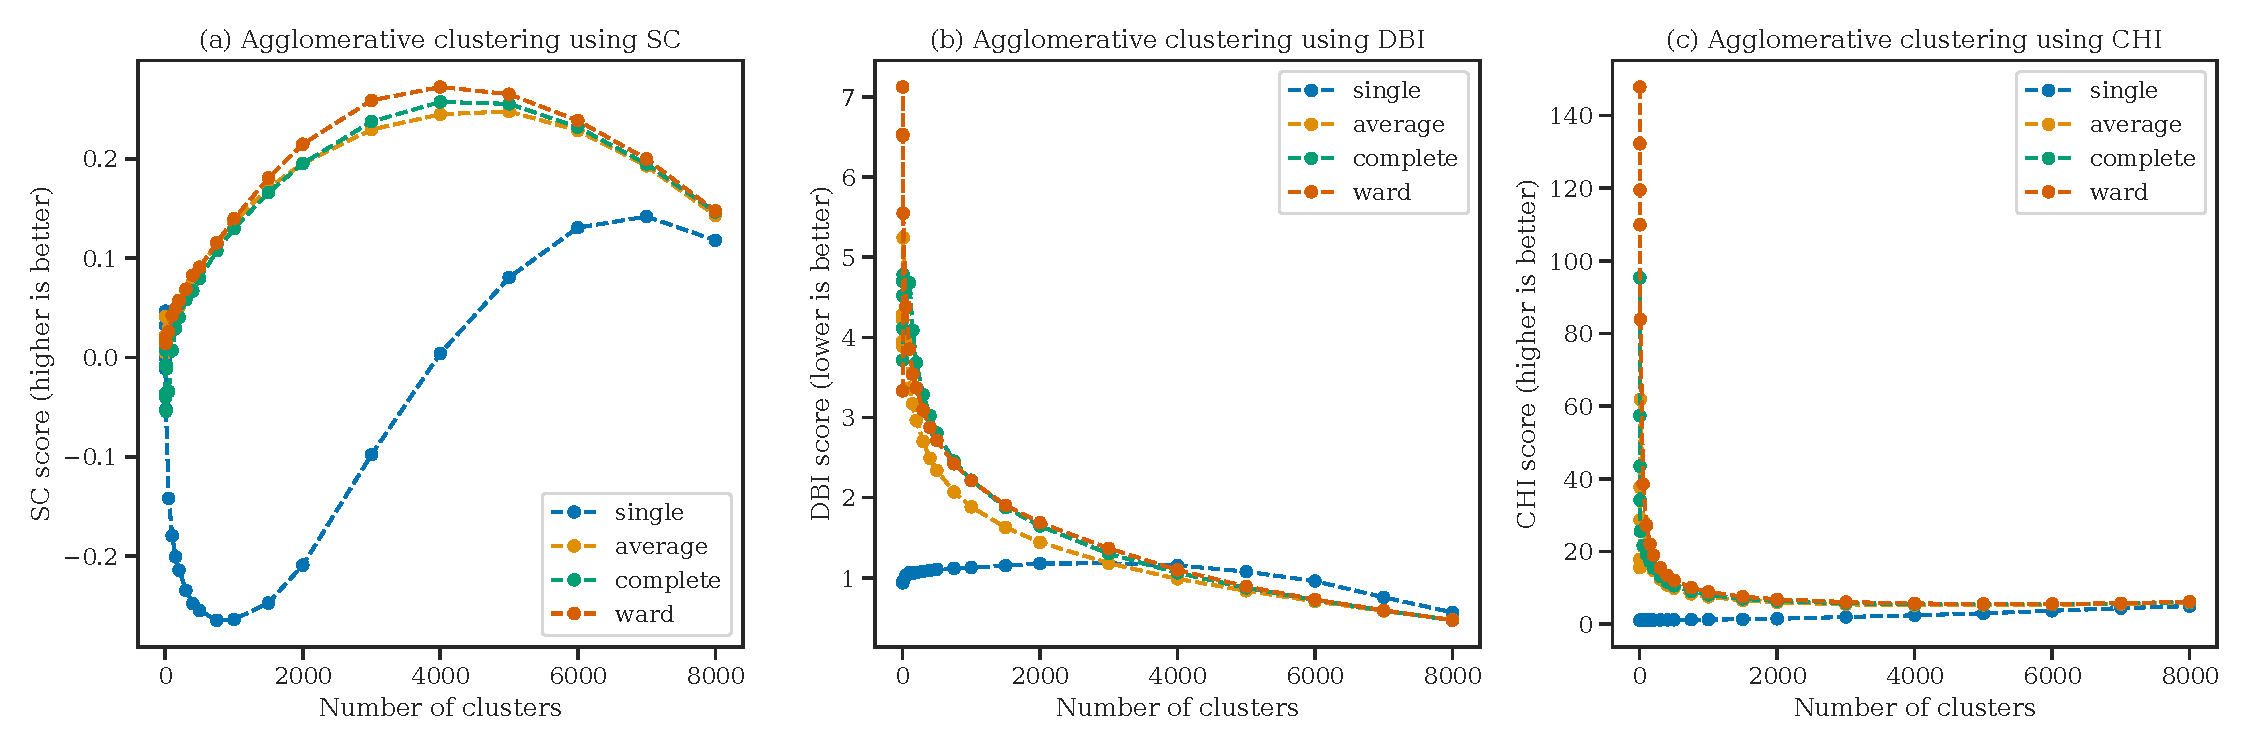
\includegraphics[width=\textwidth]{thesis/figures/cluster-analysis-agglomerative-internal-cluster-validation.pdf}
    \caption{Internal cluster validation results using agglomerative clustering on word embeddings from SGNS-enwiki.}
    \label{fig:cluster-analysis-agglomerative-internal-cluster-validation}
\end{figure}

By narrowing the search to the range 3000 to 6000 clusters, we find the best number of clusters for each criterion, using agglomerative clustering. The narrowed search for number of clusters is shown in \cref{fig:cluster-analysis-agglomerative-internal-cluster-validation-narrow}, and we observe that ward linkage clustering with 4104 clusters result in the best clustering of the 10000 most common words from the SGNS-enwiki model.
\begin{figure}[H]
    \centering
    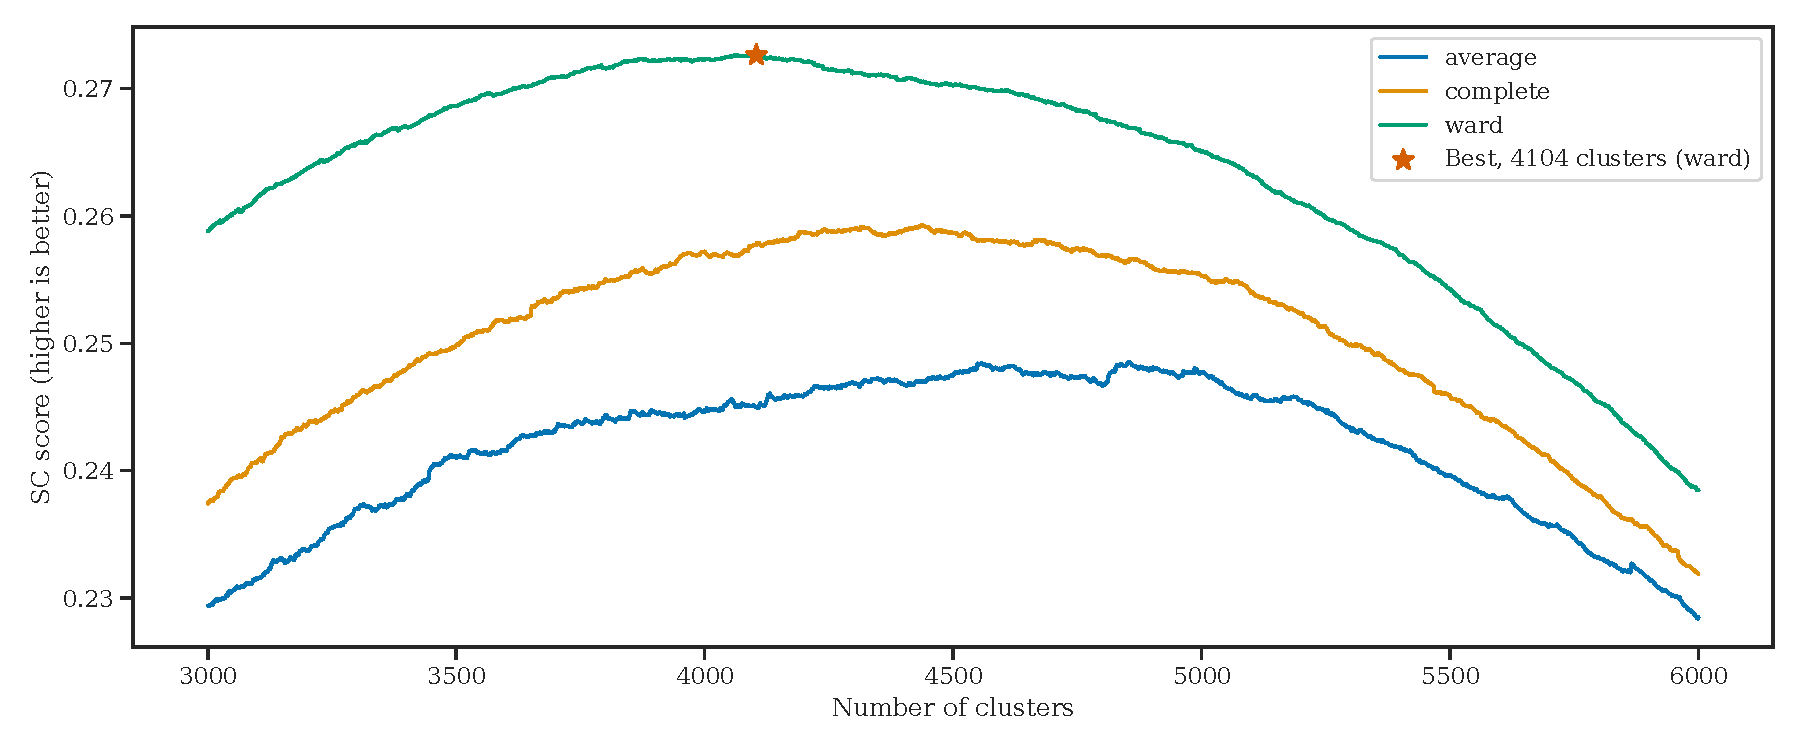
\includegraphics[width=\textwidth]{thesis/figures/cluster-analysis-agglomerative-internal-cluster-validation-narrow.pdf}
    \caption{Number of clusters search using agglomerative clustering and SC, on the range of 3000 to 6000 clusters. Here we see that ward linkage criterion results in the highest SC score.}
    \label{fig:cluster-analysis-agglomerative-internal-cluster-validation-narrow}
\end{figure}

To further gain knowledge of what the best clustering using agglomerative clustering on the word embeddings from SGNS-enwiki, we investigate the words falling into the 4104 clusters, with agglomerative clustering and ward criterion. In particular, we look at the 10 largest and smallest clusters. For the smallest clusters, we look at clusters of size 2 or more, to ensure we do not have clusters consisting of single words. In the top 10 largest clusters, we mostly see names such as "Smith", "Wilson" or "Taylor" being clustered into the same cluster. We also see words representing numbers being clustered together, e.g. "forty-five", "thirty-two" or "fifty-one", and family related words being clustered together, e.g. "father", "son" and "brother". The top 10 smallest clusters mostly consist of words that are strongly related to one another, such as "Adam" and "Noah", "card" and "cards", or "interior" and "exterior". We visualize some of the largest and smallest clusters in \cref{fig:cluster-analysis-agglomerative-2d-umap-top-clusters}, using a 2-dimensional UMAP (\cref{sec:umap}) embedding. To create the UMAP embedding, we used the \path{umap-learn} Python package \cite{mcinnes2018umap-software}, and let \path{n_neighbors=15} and \path{min_dist=0.1}. From \cref{fig:cluster-analysis-agglomerative-2d-umap-top-clusters}, we see that the clusters are widely spread all over the UMAP embedding. In addition to this, the UMAP embedding suggests that there are more clusters throughout the word embeddings, which the clustering algorithms simply were unable to pick up (when evaluated using internal cluster validation methods). We will investigate this further, and in the next subsection, we will look at clustering of distinct word groups. In particular, we will see if bigger sets of words cluster together in the UMAP embedding, suggesting that the word embeddings contains deeper structure.
\begin{figure}
    \centering
    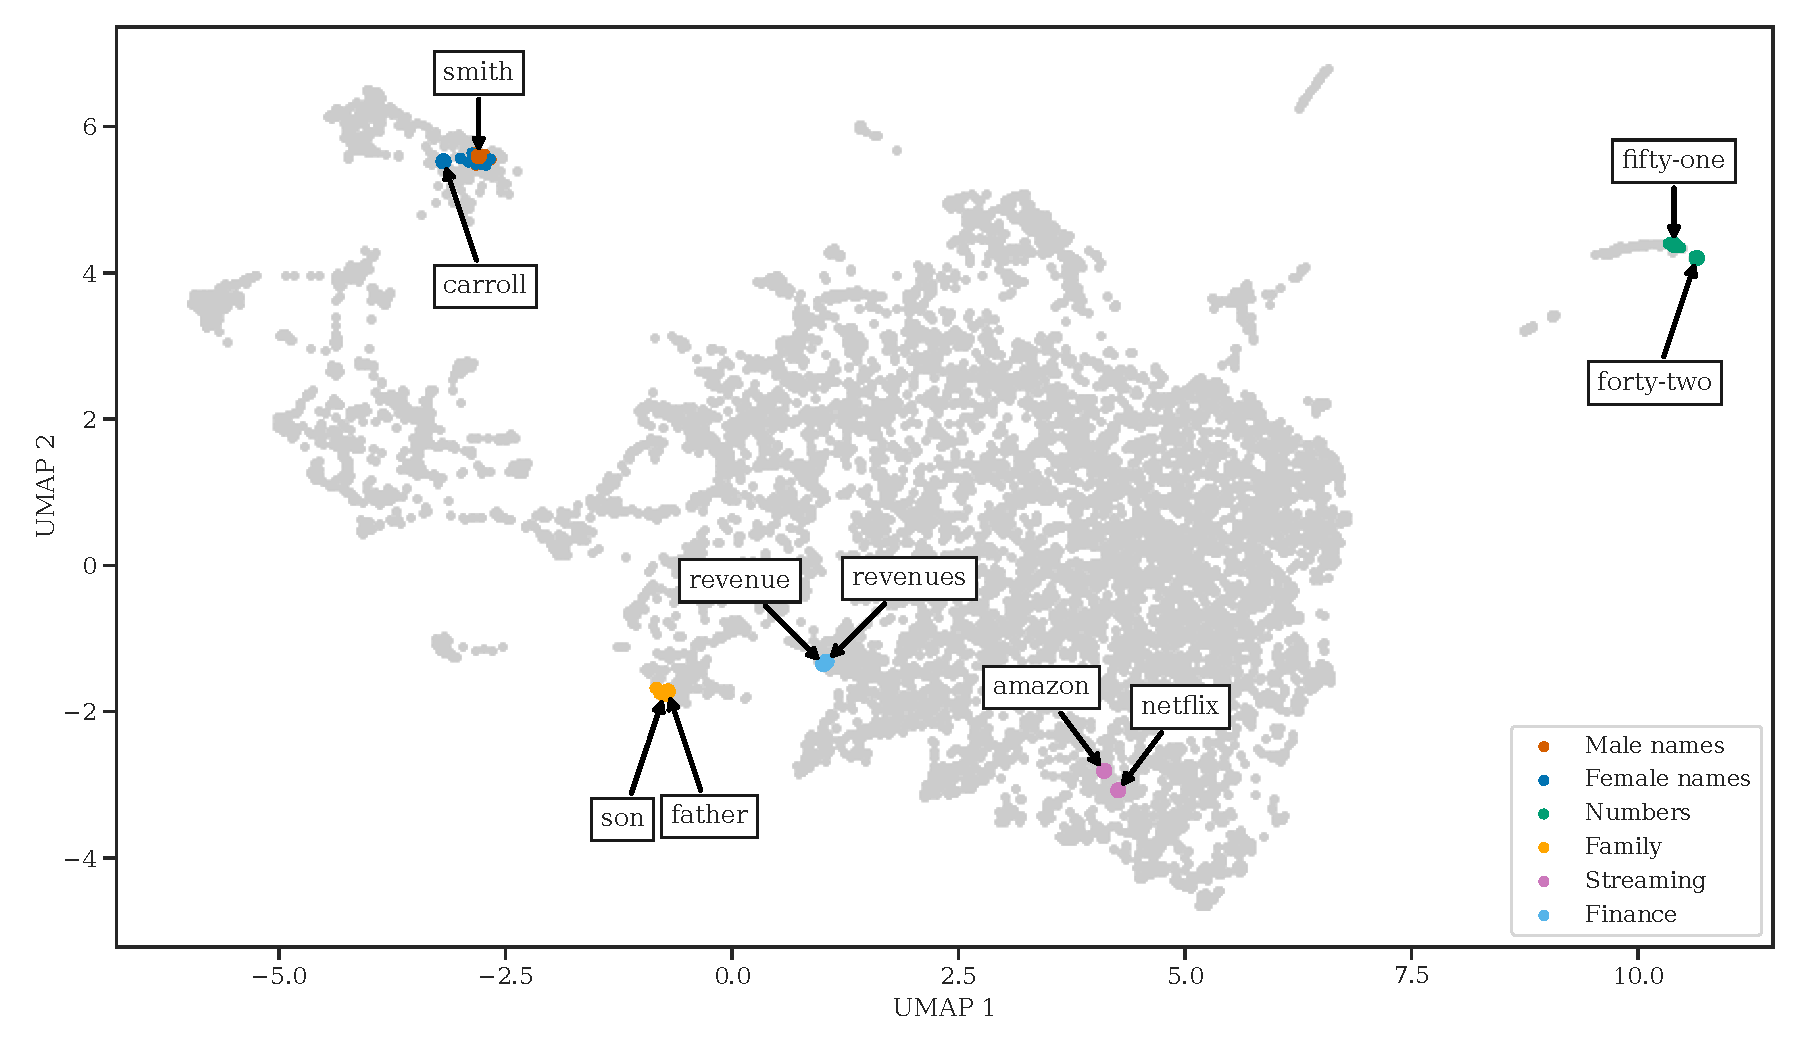
\includegraphics[width=\textwidth]{thesis/figures/cluster-analysis-agglomerative-2d-umap-top-clusters.pdf}
    \caption{2-dimensional UMAP embedding of the 10000 most common words from the SGNS-enwiki model, with some of the largest/smallest clusters outlined.}
    \label{fig:cluster-analysis-agglomerative-2d-umap-top-clusters}
\end{figure}

\subsection{Clustering word groups}
\label{sec:clustering-word-groups}
In this subsection, we will investigate the effect of clustering in the 2-dimensional UMAP embedding of the 10000 most common words of the SGNS-enwiki model, using distinct groups of words. In particular, we will cluster words related to countries/capitals, numbers, names (fore- and surnames) and food. Prior to performing the clustering, we first prepare the data to be used for the analysis. The countries/capitals data was retrieved from \cite{GeoNames}, where we used their API in order to fetch countries and its capital, resulting in 217 pairs of countries and capitals that were in the SGNS-enwiki vocabulary. The number data was generated by converting numbers to its string representation. We converted the numbers from zero to one trillion, resulting in 105 number related words. The forenames data was retrieved from \cite{SSABabyNames}, where we used the top 1000 baby names from 2019. The surnames data was retrieved from \cite{CensusSurnames}, and we used the top 1000 surnames from 2010. Finally, the food data was retrieved from \cite{FoodIngredientList}, where we used the 250 most common ingredient words. We visualize the largest clusters of word groups falling into the 10000 most common words from the SGNS-enwiki word embeddings, embedded into a 2-dimensional UMAP embeddings in \cref{fig:word-cluster-all-groups}. From \cref{fig:word-cluster-all-groups}, we observe that there are two well separated clusters forming in the UMAP embedding, namely the names and numbers word groups. The countries and food groups are more spread out in the embedding.
\begin{figure}[H]
    \centering
    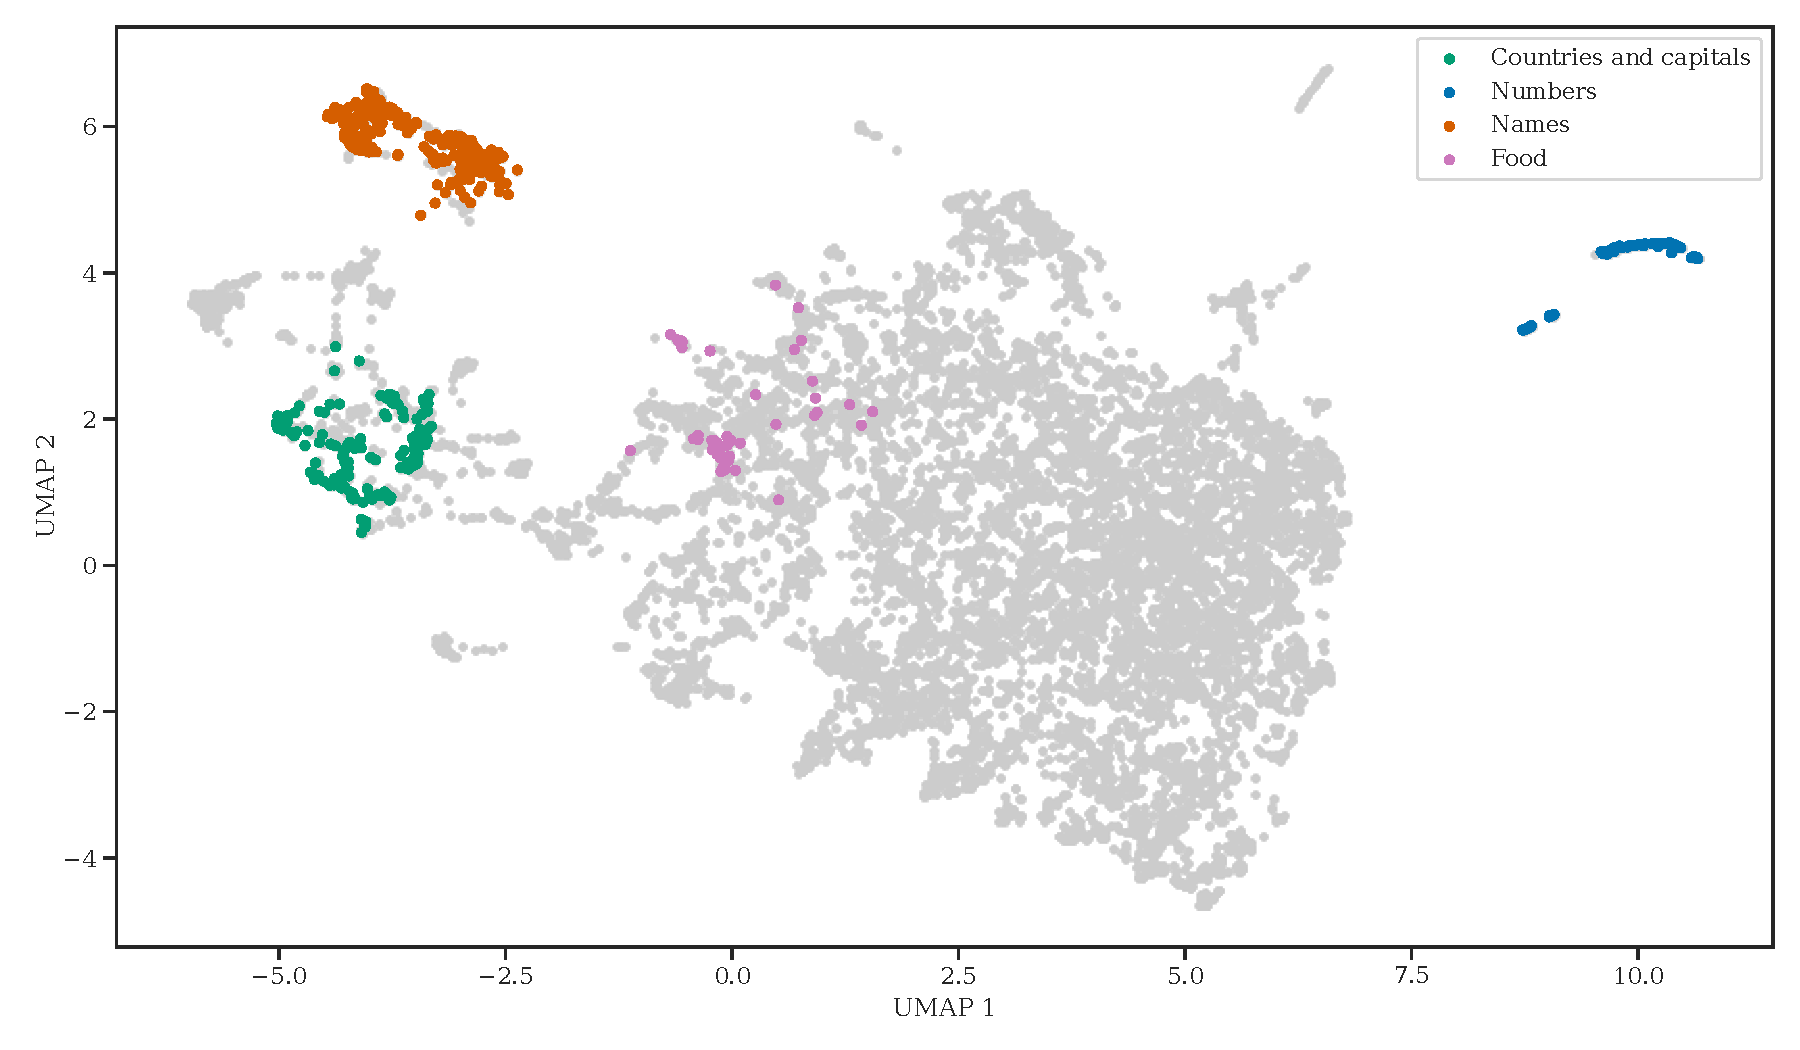
\includegraphics[width=\textwidth]{thesis/figures/word-cluster-all-groups.pdf}
    \caption{2-dimensional UMAP embedding of the 10000 most common words from the SGNS-enwiki model, with word groups outlined.}
    \label{fig:word-cluster-all-groups}
\end{figure}

Note that, in \cref{fig:word-cluster-all-groups}, we have outlined the largest clusters of the word groups, and discarded words falling out of the largest clusters. By including words that are outside the largest clusters, we saw that, in particular, the names word group is spread throughout the word embedding, as the data we used contained fore- and surnames of common words, such as "joy", "page" or "good". We illustrate this behaviour in \cref{fig:word-cluster-all-groups-emphasis-plots}, where we outline the four different word groups. From \cref{fig:word-cluster-all-groups-emphasis-plots}, we see that the country and capital words (a) are mostly clustered to the middle left, with some capitals falling out of the bigger cluster. The "Stanley" and "Hamilton" capital cities are also used as names, indicated by the names (c) plot. For the numbers, we observe that most number related words are clustered to the right, clearly separated from the rest of the words. However, we also observe that words such as "million", "billion" and "trillion" are clustered together outside the numbers cluster to the right. By inspection, we observed that the "million", "billion" and "trillion" words were in fact close to other financial words, such as "banks", "wealth" or "economics". For the names (c), we see that the fore- and surnames are clustered to the top right, but also spread throughout the UMAP embedding. We also observe a small cluster of woman names forming, containing the names "Diana" and "Isabella". Lastly, we see that food related words (d) are slightly clustered around the words "egg" and "cheese", but also slightly spread around the UMAP embedding. An interesting observation is the word "apple", which is both a fruit and a technology company. In this case, the word apple refers to the company Apple Inc., as we also saw earlier in \cref{table:word2vec-nearest-neighbours-words}.
\begin{figure}[H]
    \centering
    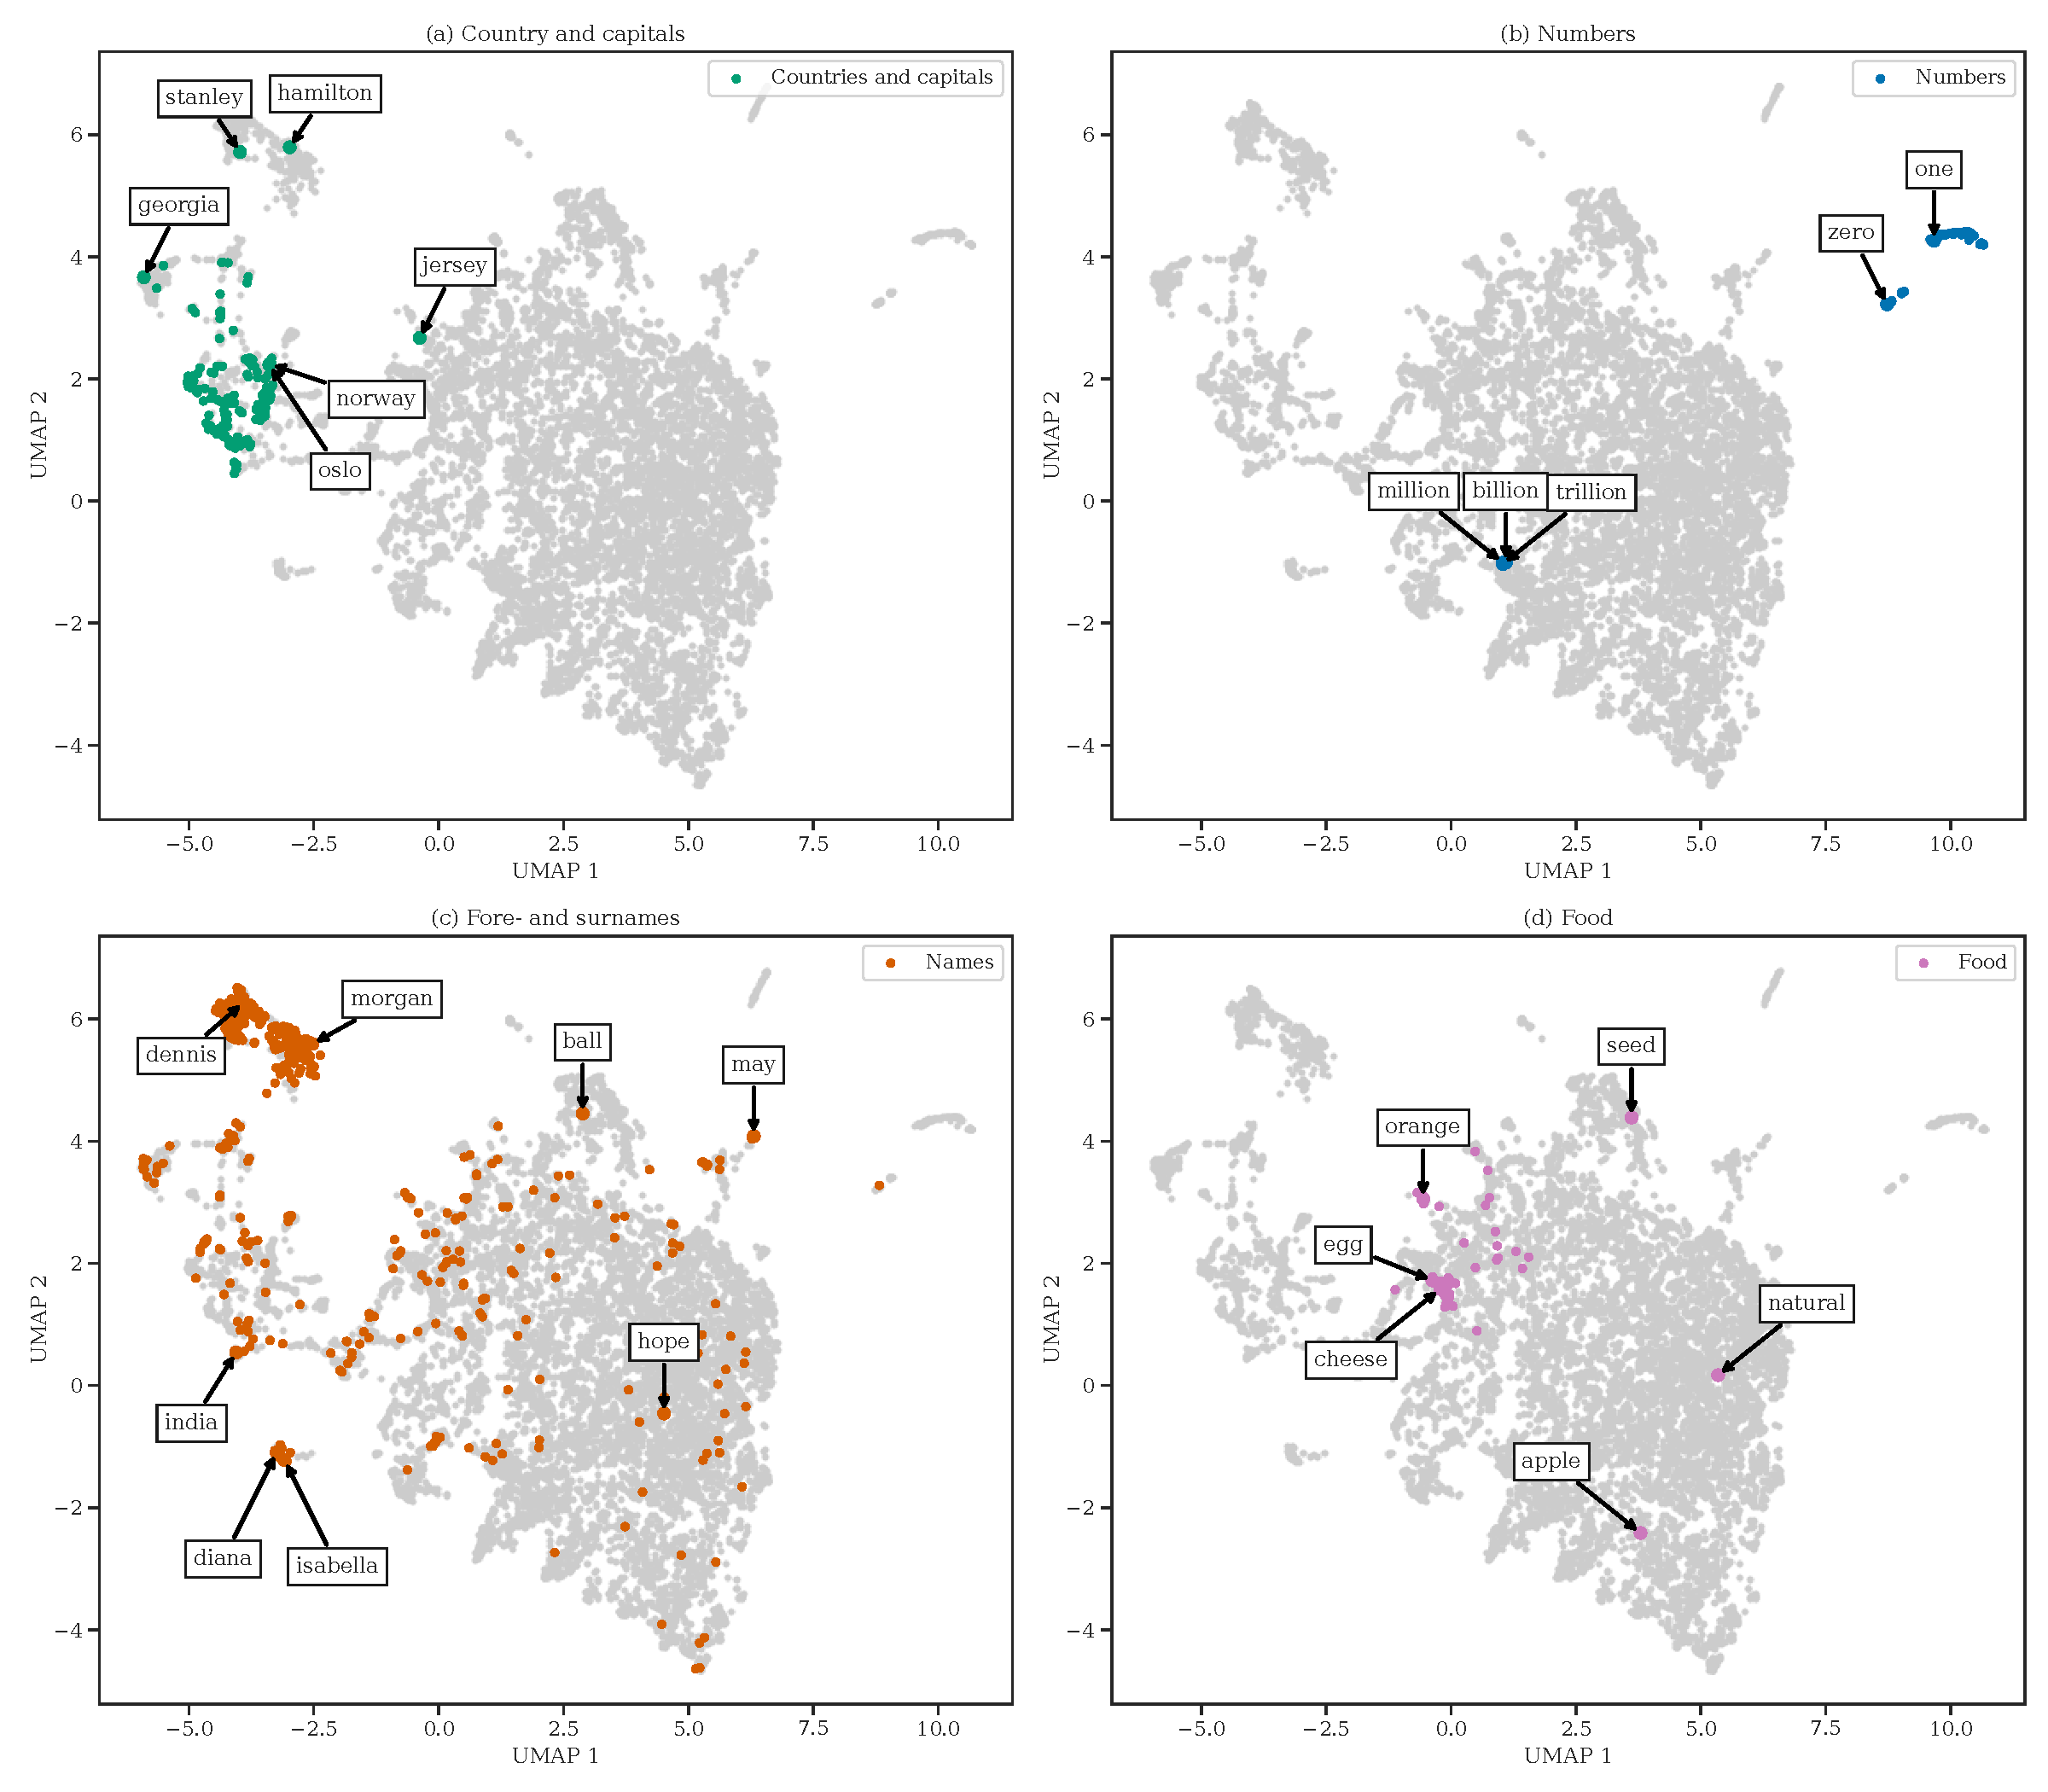
\includegraphics[width=\textwidth]{thesis/figures/word-cluster-all-groups-emphasis-plots.pdf}
    \caption{2-dimensional UMAP embeddings of the 10000 most common words from the SGNS-enwiki model. Here we see four plots, where in each plot we have outlined the four different word groups.}
    \label{fig:word-cluster-all-groups-emphasis-plots}
\end{figure}

We will now further analyze two of the word groups to further develop our understanding of the word embeddings. In particular, we will perform cluster analysis of the word embeddings of countries/capitals and numbers, where we will use clustering algorithms to cluster the words. We will use the same clustering algorithms specified in \cref{sec:comparing-clustering-algorithms}, in addition to Spectral clustering. In order to visualize the results, we will use dimensionality reduction algorithms to create 2-dimensional embeddings. We will also use latitude/longitude coordinates of countries in order to visualize the clustering results using countries/capitals word embeddings.

We analyze the countries and capital word groups separately, as we choose to either identify a country by its name or its capital. Starting with the country word group, we perform cluster analysis. The result of the cluster analysis is summarized in \cref{fig:cluster-analysis-country-word-group-internal-cluster-validation}. There we see a similar result to the result shown in \cref{fig:cluster-analysis-comparison-internal-cluster-validation}, namely that agglomerative clustering is the preferred choice of clustering algorithm.
\begin{figure}[H]
    \centering
    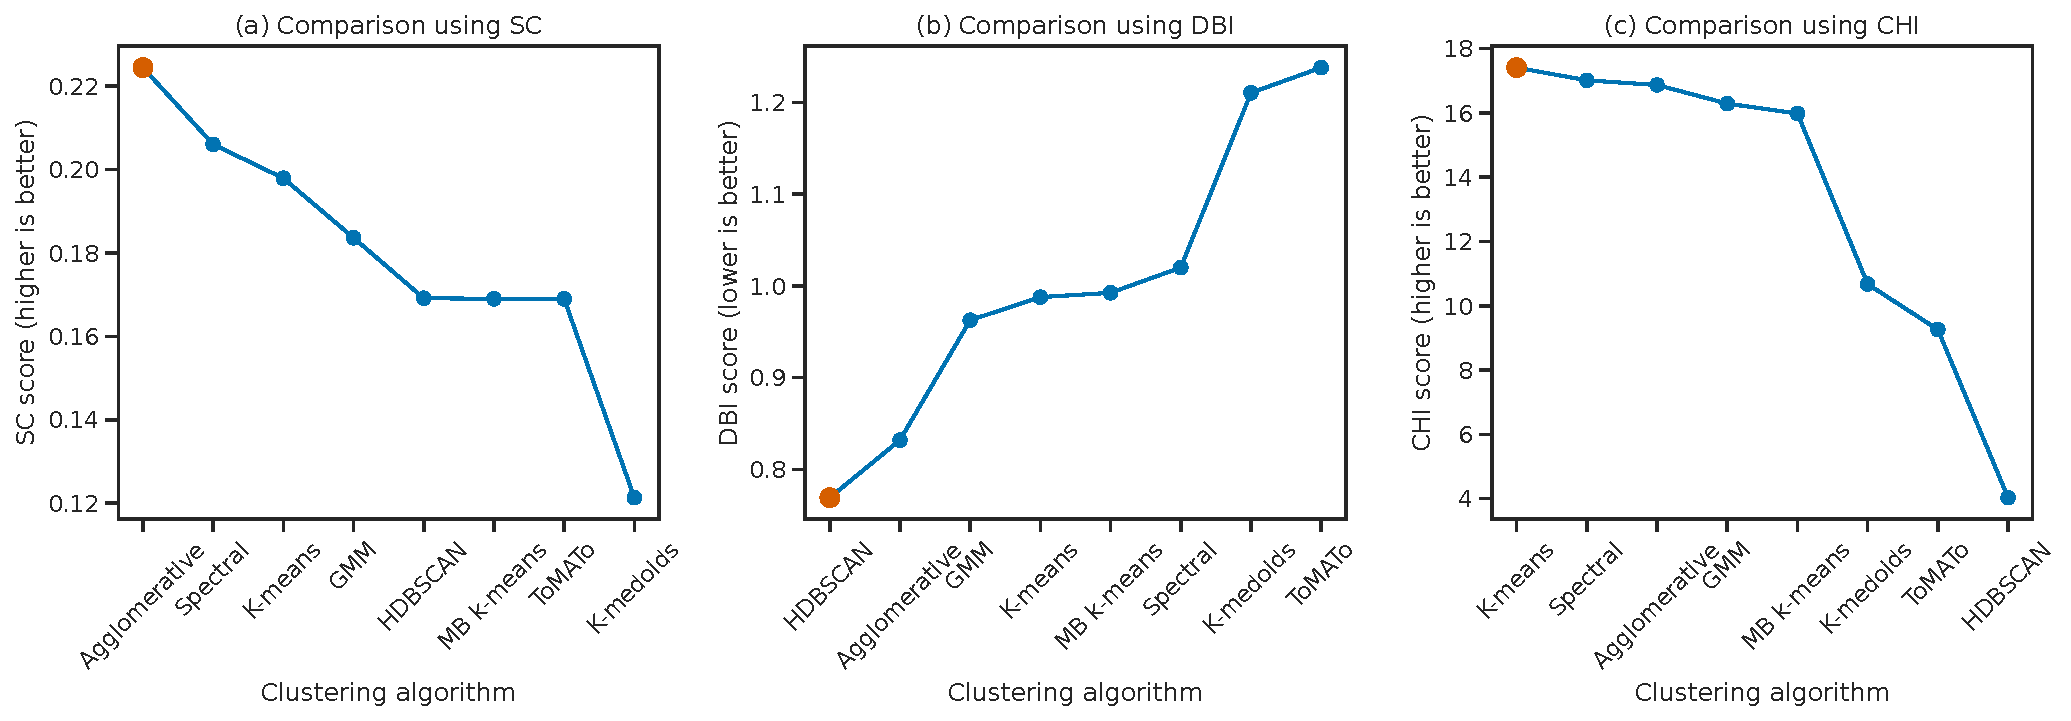
\includegraphics[width=\textwidth]{thesis/figures/cluster-analysis-country-word-group-internal-cluster-validation.pdf}
    \caption{Comparison of clustering algorithms trained on country word embeddings from SGNS-enwiki, ranked by internal cluster validation methods. The red dot in each plot denotes the most optimal value.}
    \label{fig:cluster-analysis-country-word-group-internal-cluster-validation}
\end{figure}

Following, we inspected the scores from the DBI and CHI methods and observed a similar pattern to the analysis from \cref{sec:comparing-clustering-algorithms}, namely that DBI prefers every word to be in its own cluster and CHI prefers to have the smallest number of clusters (i.e. 2). For this reason, we mainly focus on the results using SC. Using agglomerative clustering, we visualize its result in \cref{fig:cluster-analysis-agglomerative-country-word-group-internal-cluster-validation}. From \cref{fig:cluster-analysis-agglomerative-country-word-group-internal-cluster-validation}, we see similar results to \cref{fig:cluster-analysis-agglomerative-internal-cluster-validation}, namely that ward criterion gives the best clustering when using agglomerative clustering.
\begin{figure}[H]
    \centering
    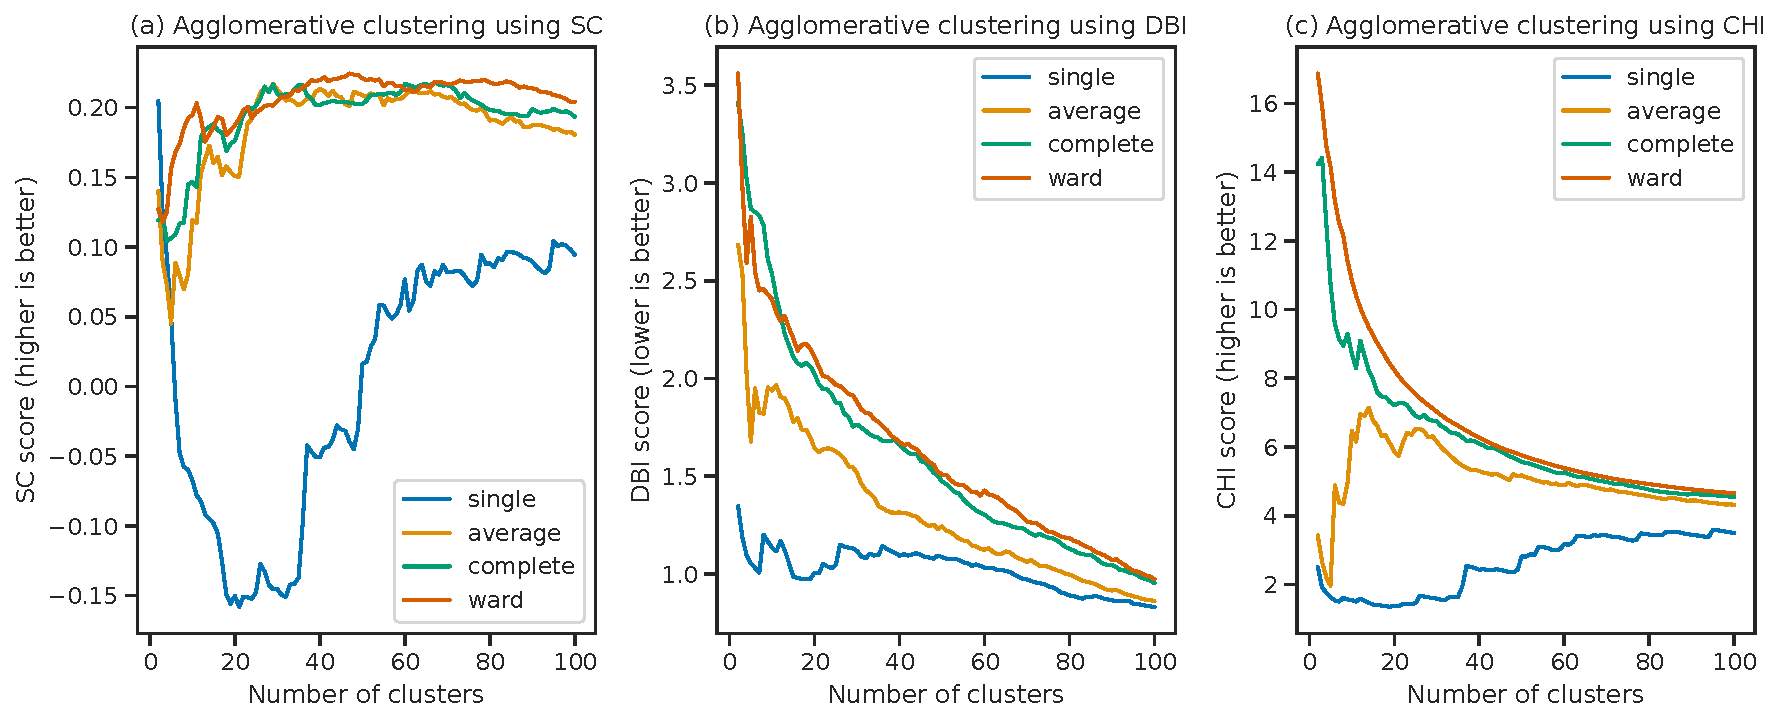
\includegraphics[width=\textwidth]{thesis/figures/cluster-analysis-agglomerative-country-word-group-internal-cluster-validation.pdf}
    \caption{Internal cluster validation results using agglomerative clustering on country word embeddings from SGNS-enwiki.}
    \label{fig:cluster-analysis-agglomerative-country-word-group-internal-cluster-validation}
\end{figure}

The best clustering using SC with agglomerative clustering and ward criterion resulted in 47 clusters. We visualize this result using latitude/longitude coordinates of each country by emphasizing the five largest clusters in \cref{fig:cluster-analysis-agglomerative-country-word-group-top-clusters}. From \cref{fig:cluster-analysis-agglomerative-country-word-group-top-clusters}, we see that the top 5 largest clusters are clustered together in the same continent.
\begin{figure}[H]
    \centering
    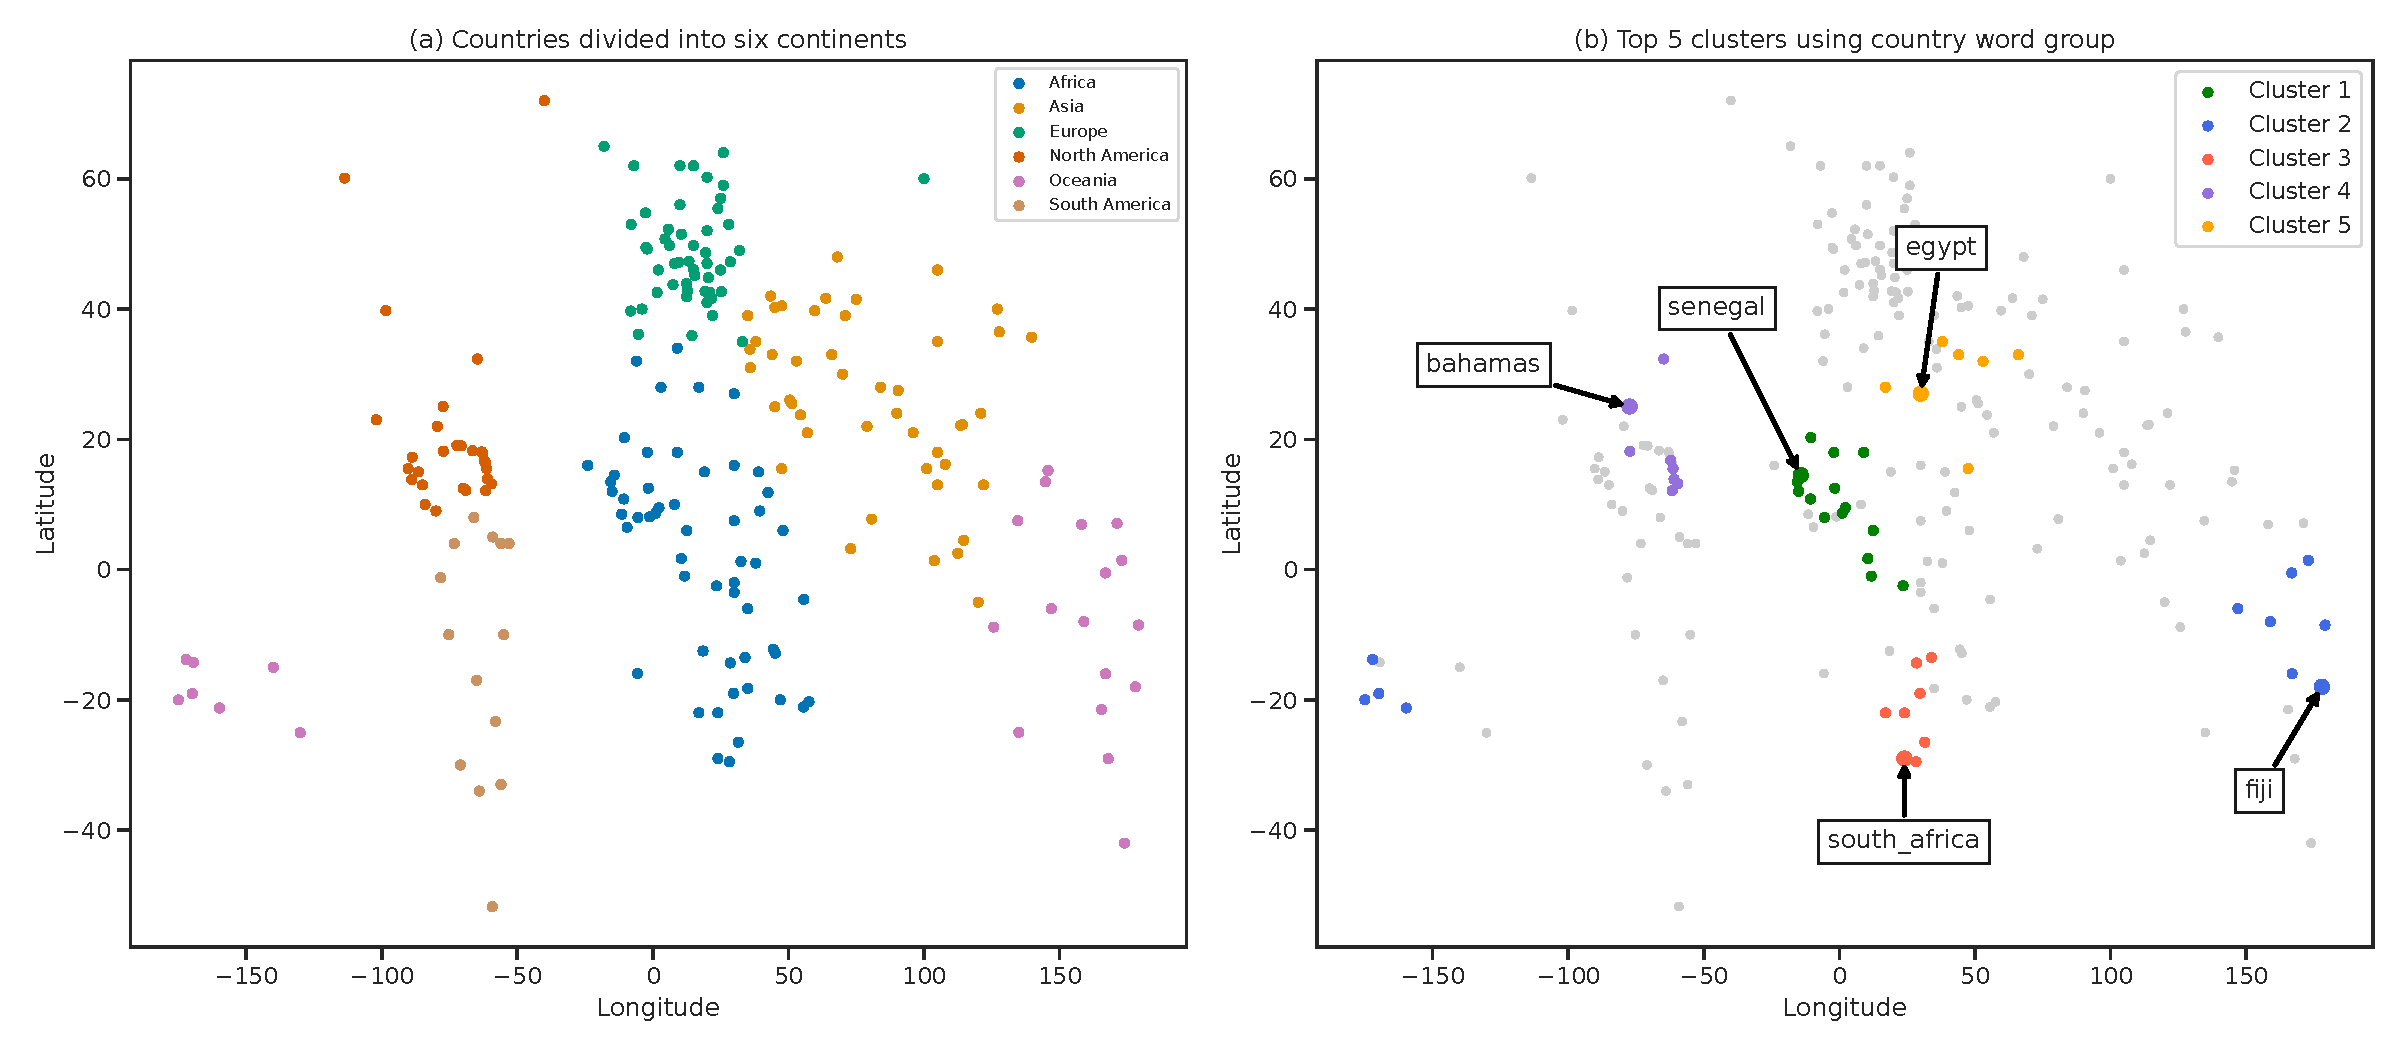
\includegraphics[width=\textwidth]{thesis/figures/cluster-analysis-agglomerative-country-word-group-top-clusters.pdf}
    \caption{Comparison of countries clustered into their respective continents (a) versus top 5 largest clusters from clustering of country word embeddings from SGNS-enwiki using agglomerative clustering and ward criterion. Here we can see that the top 5 largest clusters using agglomerative clustering correlate well with the continent of the respective countries.}
    \label{fig:cluster-analysis-agglomerative-country-word-group-top-clusters}
\end{figure}

Furthermore, we repeat the cluster analysis using capital to identify each country. That is, we use the word embeddings of the capital words instead of the previously used country word embeddings. The result of the cluster analysis is summarized in \cref{fig:cluster-analysis-country-capitals-word-group-internal-cluster-validation}. There we see a similar result to the result shown in both \cref{fig:cluster-analysis-comparison-internal-cluster-validation} and \cref{fig:cluster-analysis-country-word-group-internal-cluster-validation}, namely that agglomerative clustering is the preferred choice of clustering algorithm.
\begin{figure}[H]
    \centering
    \includegraphics[width=\textwidth]{thesis/figures/cluster-analysis-country-capitals-word-group-internal-cluster-validation.pdf}
    \caption{Comparison of clustering algorithms trained on capital word embeddings from SGNS-enwiki, ranked by internal cluster validation methods. The red dot in each plot denotes the most optimal value.}
    \label{fig:cluster-analysis-country-capitals-word-group-internal-cluster-validation}
\end{figure}

We inspected the scores from the DBI and CHI methods, and similar to the results from \cref{sec:comparing-clustering-algorithms} and the cluster analysis using country word embeddings, we saw that DBI prefers every word to be in its own cluster and CHI prefers to have the smallest number of clusters (i.e. 2). This further strengthens the motivation to use SC over the other methods, and we mainly focus on the results using SC. Using agglomerative clustering, we visualize the results using capital word embeddings in \cref{fig:cluster-analysis-agglomerative-country-capitals-word-group-internal-cluster-validation}. From \cref{fig:cluster-analysis-agglomerative-country-capitals-word-group-internal-cluster-validation}, we see similar results to \cref{fig:cluster-analysis-agglomerative-internal-cluster-validation} and \cref{fig:cluster-analysis-agglomerative-country-word-group-internal-cluster-validation}, namely that ward criterion gives the best clustering when using agglomerative clustering.
\begin{figure}[H]
    \centering
    \includegraphics[width=\textwidth]{thesis/figures/cluster-analysis-agglomerative-country-capitals-word-group-internal-cluster-validation.pdf}
    \caption{Internal cluster validation results using agglomerative clustering on capital word embeddings from SGNS-enwiki.}
    \label{fig:cluster-analysis-agglomerative-country-capitals-word-group-internal-cluster-validation}
\end{figure}

The best clustering using SC with agglomerative clustering and ward criterion resulted in 21 clusters. We visualize this result using latitude/longitude coordinates of each country by emphasizing the five largest clusters in \cref{fig:cluster-analysis-agglomerative-country-capitals-word-group-top-clusters}. From \cref{fig:cluster-analysis-agglomerative-country-capitals-word-group-top-clusters}, we see that we get larger clusters than by using country word embeddings in \cref{fig:cluster-analysis-agglomerative-country-word-group-top-clusters}. Furthermore, we observe that in plot (b) the first cluster (green) consists of capitals where the countries are Spanish talking, as outlined by the "Madrid" (Spain), "Mexico City" (Mexico) and "Santiago" (Chile) boxes. The second cluster (blue) in plot (b) also correlates well with the Oceanic continent of plot (a), while the third (red) and forth (purple) clusters of plot (b) seem to capture the African continent very well (Dakar is the capital of Senegal and Pretoria is one of the capitals of South Africa). The last cluster (yellow) consists of capitals from Eastern Europe, as well as some Asian capitals. This concludes the cluster analysis of country and capital word embeddings, and furthermore, we will perform cluster analysis of words related to numbers.
\begin{figure}[H]
    \centering
    \includegraphics[width=\textwidth]{thesis/figures/cluster-analysis-agglomerative-country-capitals-word-group-top-clusters.pdf}
    \caption{Comparison of countries clustered into their respective continents (a) versus top 5 largest clusters from clustering of capital word embeddings from SGNS-enwiki using agglomerative clustering and ward criterion. From plot (b) we can see that Spanish speaking countries are clustered together in the first cluster (green), while the other clusters are well clustered with regards to the continent of its country.}
    \label{fig:cluster-analysis-agglomerative-country-capitals-word-group-top-clusters}
\end{figure}

We perform cluster analysis of number word embeddings in a similar manner to the cluster analysis of country/capital word embeddings. First, we compare clustering algorithms using internal cluster validation methods, as shown in \cref{fig:cluster-analysis-numbers-word-group-internal-cluster-validation}. From \cref{fig:cluster-analysis-numbers-word-group-internal-cluster-validation}, we see that, overall, the agglomerative clustering algorithm is the best clustering algorithm, when evaluated using internal validation methods.
\begin{figure}[H]
    \centering
    \includegraphics[width=\textwidth]{thesis/figures/cluster-analysis-numbers-word-group-internal-cluster-validation.pdf}
    \caption{Comparison of clustering algorithms trained on number word embeddings from SGNS-enwiki, ranked by internal cluster validation methods. The red dot in each plot denotes the most optimal value.}
    \label{fig:cluster-analysis-numbers-word-group-internal-cluster-validation}
\end{figure}

Furthermore, we use the agglomerative clustering algorithm. To find its best criterion and number of clusters, we first visualize its results in \cref{fig:cluster-analysis-agglomerative-numbers-word-group-internal-cluster-validation}. From \cref{fig:cluster-analysis-agglomerative-numbers-word-group-internal-cluster-validation}, we see that SC (a) prefers complete linkage criterion with 2 clusters, DBI (b) prefers single linkage criterion with 6 clusters and CHI (c) prefers ward linkage criterion with 3 clusters. In other words, we here see a different behaviour of the internal cluster validation methods than in \cref{sec:comparing-clustering-algorithms} and the country/capital cluster analysis, namely that SC prefers the least amount of clusters, DBI does not prefer the most amount of clusters and CHI does not prefer the least amount of clusters.
\begin{figure}[H]
    \centering
    \includegraphics[width=\textwidth]{thesis/figures/cluster-analysis-agglomerative-numbers-word-group-internal-cluster-validation.pdf}
    \caption{Internal cluster validation results using agglomerative clustering on number word embeddings from SGNS-enwiki.}
    \label{fig:cluster-analysis-agglomerative-numbers-word-group-internal-cluster-validation}
\end{figure}

To understand which internal clustering validation method from \cref{fig:cluster-analysis-agglomerative-numbers-word-group-internal-cluster-validation} performs the best, we visualize the result using the best clustering of each of them in three subplots, as show in \cref{fig:cluster-analysis-agglomerative-numbers-word-group-internal-cluster-validation-best-2d-pca}. From \cref{fig:cluster-analysis-agglomerative-numbers-word-group-internal-cluster-validation-best-2d-pca}, we see that it is not entirely clear how to cluster the number word embeddings.
\begin{figure}[H]
    \centering
    \includegraphics[width=\textwidth]{thesis/figures/cluster-analysis-agglomerative-numbers-word-group-internal-cluster-validation-best-2d-pca.pdf}
    \caption{Comparison of the best result given by internal cluster validation methods using agglomerative clustering on number word embeddings from SGNS-enwiki. Here we see that it is not clear which clustering is the best.}
    \label{fig:cluster-analysis-agglomerative-numbers-word-group-internal-cluster-validation-best-2d-pca}
\end{figure}

We further investigated the structure of the 2-dimensional PCA embedding of the number words, and noticed an interesting relationship. This relationship is illustrated in \cref{fig:ordered-number-word-embeddings-2d-pca} and shows that if we assign an increasing label from the smallest and to the largest number, we see the color of the label gradually increasing from the smallest label color to the largest label color. In other words, there seems to be an underlying sequential relationship to the word embeddings. Furthermore, this suggests that the underlying structure of number word embeddings may contain information which we have not been able to find yet.
\begin{figure}[H]
    \centering
    \includegraphics[width=\textwidth]{thesis/figures/ordered-number-word-embeddings-2d-pca.pdf}
    \caption{2-dimensional PCA embedding of the 105 number word embeddings, where each word embedding have an increasing label assigned to it. Here we see that as we increase the number, we see a possible underlying sequential relationship.}
    \label{fig:ordered-number-word-embeddings-2d-pca}
\end{figure}
\section{Polysemous words prediction}
\label{sec:polysemous-words-prediction}
In this section, we try to predict whether or not a word is polysemous, given its word vector. We will, first, apply methods from topological data analysis to word embeddings. In particular, we will investigate the notion of topological polysemy in \cref{sec:analysis-of-embeddings-topological-polysemy} and geometric anomaly detection in \cref{sec:analysis-of-embeddings-geometric-anomaly-detection}. We use topological polysemy to attempt to estimate the number of meanings of a word, given its word vector; we would like to see if the $\text{TPS}_n(w)$ score actually measures polysemy. In addition to this, we would like to see if singular word vectors, as identified by geometric anomaly detection, are polysemous as well. Following, we compute the estimated intrinsic dimension of word embeddings and compare the results with the number of word meanings in \cref{sec:analysis-of-embeddings-intrinsic-dimension-estimation}. Finally, we propose supervised models to predict the number of word meanings in \cref{sec:analysis-of-embeddings-supervised-polysemy-prediction}.

\subsection{Topological polysemy}
\label{sec:analysis-of-embeddings-topological-polysemy}
In this subsection, we apply topological polysemy (\cref{sec:topological-polysemy}) to the word embeddings from SGNS-enwiki. We will also train another word2vec model using the same training data used by \cite{jakubowski2020topology} and apply topological polysemy to its word embeddings. We refer to this word2vec model as the \textit{SGNS-semeval} model. Furthermore, we compare the results to topological polysemy applied to word embeddings from pre-trained models, namely the fastText model (\textit{fastText.TPS.300d}) used in experiments of \cite{jakubowski2020topology}, the \textit{GoogleNews-vectors-negative300} (shortened to \textit{GoogleNews300}) word embeddings from \cite{GoogleCodeArchiveWord2vec}, the \textit{glove.840B.300d} word embeddings from \cite{GloVeProject2014} and the English (\textit{fastText.en.300d}) word embeddings from \cite{grave2018learning}. The fastText.TPS.300d model was kindly given in private communication with one of the authors of topological polysemy \cite{ZibrowiusPrivComs2021}.

The authors of topological polysemy, \cite{jakubowski2020topology}, trained a fastText model on training data from the \textit{SemEval-2010 Task 14: Evaluation Setting for Word Sense Induction \& Disambiguation Systems} \cite{manandhar-klapaftis-2009-semeval}. The training data from the SemEval task consists of several sentences related to 100 polysemous words (50 nouns and 50 verbs). The SemEval data set also includes the number of true meanings (also called \textit{gold standard} or \textit{GS}) for each of the 100 polysemous words, as perceived by humans. In private communication with one of the authors of topological polysemy \cite{ZibrowiusPrivComs2021}, they stated that they used a fastText model with vector dimensionality of 300, and to process the training data, they removed all punctuation and replaced capital letters by the corresponding small letters. To compare with the $\text{TPS}_n(w)$, the authors use the 100 polysemous words, words from the SemEval training data which has a \textit{WordNet} \cite{fellbaum1998} entry and all words in SemEval training data. WordNet is a lexical database of the English language. In particular, it allows for querying nearly any word from the English language and and returns the \textit{synsets} of the word. Synsets of a query word $w$ is a collection of words which have similar meaning as the word $w$. In other words, by querying a word in WordNet, we can get the number of meanings of a word, as perceived by WordNet. Furthermore, the Pearson correlation coefficient \cite{James2013} is computed between $\text{TPS}_n(w)$ and GS, the number of synsets for WordNet words and the word frequency as they appear in the SemEval training data, respectively. The authors show that there is a moderate (positive) correlation between $\text{TPS}_n(w)$ and GS at $n \in \enclc{40, 50, 60}$, a decreasing correlation between $\text{TPS}_n(w)$ and the number of synsets for WordNet words and no correlation between $\text{TPS}_n(w)$ and word frequencies. In our implementation of topological polysemy, we utilized multiprocessing and the ScaNN \cite{scann2020} approximate nearest neighbour algorithm to speed up the computation. ScaNN was chosen because it performs well when applied to word embeddings, as shown in \cite{AnnBenchmarks2021}. We used the \path{ripser} \cite{ctralie2018ripser} Python package to compute Vietoris–Rips complexes. \textbf{TODO}: Ripser or Gudhi?

We trained the SGNS-semeval model using the training data from the SemEval task and the hyperparameters used to train the SGNS-enwiki model from \cref{sec:word2vec-hyperparameter-choices}. This resulted in a vocabulary size of $\sim$122K words and corpus size of $\sim$67 million for the SGNS-enwiki model. Following, we will compare the results from the experiments of \cite{jakubowski2020topology} by computing topological polysemy at varying levels of $n$ using the word embeddings of SGNS-enwiki and SGNS-semeval. Finally, we compare the results using the SGNS-enwiki and SGNS-semeval word embeddings to the word embeddings of the fastText.TPS.300d, GoogleNews300, glove.840B.300d and fastText.en.300d models.

The results of computing topological polysemy at varying levels of $n$ using the word embeddings of SGNS-enwiki and SGNS-semeval are shown in \cref{table:tps-n-correlation-sgns-enwiki,table:tps-n-correlation-sgns-semeval}. From \cref{table:tps-n-correlation-sgns-enwiki}, we see that the correlation between $\text{TPS}_n$ and GS is rather stable with respect to $n$. In particular, we notice that the correlation between $\text{TPS}_n$ and GS is negative, suggesting a relationship in the opposite direction of the results from \cite[Table 1]{jakubowski2020topology}. Nonetheless, we see a decreasing correlation when comparing $\text{TPS}_n$ versus the number of WordNet synsets for each word, and a negligible correlation between $\text{TPS}_n$ and word frequencies of the top 10000 most common words. Furthermore, from \cref{table:tps-n-correlation-sgns-semeval}, we observe a decreasing negative correlation (towards zero) between $\text{TPS}_n$ and GS, meaning that the SGNS-semeval model performs worse than the SGNS-enwiki model on this particular task. This may indicate that by training SGNS-semeval on a smaller vocabulary than the vocabulary of SGNS-enwiki we get worse results. Furthermore, we see a a decreasing correlation between $\text{TPS}_n$ and the number of WordNet synsets and a negligible correlation between $\text{TPS}_n$ and word frequencies of the top 10000 most common words. Although the negative correlation between $\text{TPS}_n$ and the number of WordNet synsets is larger for the SGNS-semeval model than the SGNS-enwiki model, it is still not particularly large. In addition to this, we are considering a lot fewer words when computing the correlation in the SGNS-semeval model than the SGNS-enwiki model (see sample size).
\begin{table}[H]
    \centering
    \begin{tabular}{@{}rrrr@{}}
    \toprule
    $n$ & $\text{TPS}_n$ vs. GS & $\text{TPS}_n$ vs. synsets & $\text{TPS}_n$ vs. frequency \\
    \midrule
    \trcolor 10  & -0.353        & -0.077             & \textbf{-0.043}               \\
    40  & \textbf{-0.383}        & -0.181             & -0.041               \\
    \trcolor 50  & -0.380        & -0.190             & -0.041               \\
    60  & -0.381        & -0.196             & -0.040               \\
    \trcolor 100 & -0.380        & \textbf{-0.205}             & -0.033               \\
    \midrule
    \textit{sample size} & 98 & 144 412 & 10 000 \\
    \bottomrule
    \end{tabular}
    \caption{Correlations between $\text{TPS}_n$ and the number of word meanings as perceived by humans (GS), the number of WordNet synsets and the word frequencies of the top 10000 most common words from the SGNS-enwiki model. \textbf{Bold} values indicate the largest (absolute) correlation.}
    \label{table:tps-n-correlation-sgns-enwiki}
\end{table}
\begin{table}[H]
    \centering
    \begin{tabular}{@{}rrrr@{}}
    \toprule
    $n$ & $\text{TPS}_n$ vs. GS & $\text{TPS}_n$ vs. synsets & $\text{TPS}_n$ vs. frequency \\
    \midrule
    \trcolor 10  & \textbf{-0.300}        & -0.248             & 0.102                \\
    40  & -0.201        & -0.300             & \textbf{0.120}                \\
    \trcolor 50  & -0.194        & -0.304             & 0.116                \\
    60  & -0.169        & -0.306             & 0.110                \\
    \trcolor 100 & -0.130        & \textbf{-0.310}             & 0.098                \\
    \midrule
    \textit{sample size} & 100 & 62 111 & 10 000 \\
    \bottomrule
    \end{tabular}
    \caption{Correlations between $\text{TPS}_n$ and the number of word meanings as perceived by humans (GS), the number of WordNet synsets and the word frequencies of the top 10000 most common words from the SGNS-semeval model. \textbf{Bold} values indicate the largest (absolute) correlation.}
    \label{table:tps-n-correlation-sgns-semeval}
\end{table}

To further broaden our understanding of the results from computing topological polysemy of the word embeddings of the SGNS-enwiki and the SGNS-semeval model, we plot $\text{TPS}_n(w)$ against the GS, the number of WordNet synsets and word frequencies, as shown in \cref{fig:tps-n-correlation-sgns-enwiki,fig:tps-n-correlation-sgns-semeval}. For each plot, we let $n$ be equal to the most optimal value for each column in \cref{table:tps-n-correlation-sgns-enwiki,table:tps-n-correlation-sgns-semeval}. From \cref{table:tps-n-correlation-sgns-enwiki}, we see a similar situation to the results from \cite[Figures 8 and 9]{jakubowski2020topology}, namely that in plot (a) we see an indication of a linear relationship between $\text{TPS}_n(w)$ and the SemEval gold standard and in plot (b) we see a clear trend between $\text{TPS}_n(w)$ and the number of synsets in WordNet. In plot (c) it is clear that there is no apparent relationship between $\text{TPS}_n(w)$ and the word frequencies. Following, we see a similar situation appearing in \cref{table:tps-n-correlation-sgns-enwiki}. These results suggest that, even by computing $\text{TPS}_n(w)$ of the SGNS-enwiki word embeddings, which has a vocabulary much larger than in the experiments of \cite{jakubowski2020topology}, we are unable to use $\text{TPS}_n(w)$ alone for predicting the number of word meanings, as given by the number of WordNet synsets.
\begin{figure}[H]
    \centering
    \includegraphics[width=\textwidth]{thesis/figures/tps-n-correlation-sgns-enwiki.pdf}
    \caption{Topological polysemy $\text{TPS}_n(w)$ of the word embeddings of SGNS-enwiki plotted against the GS (a), the number of WordNet synsets (b) and word frequencies (c). Plots are inspired by \cite[Figures 8 and 9]{jakubowski2020topology}.}
    \label{fig:tps-n-correlation-sgns-enwiki}
\end{figure}
\begin{figure}[H]
    \centering
    \includegraphics[width=\textwidth]{thesis/figures/tps-n-correlation-sgns-semeval_2010_task_14.pdf}
    \caption{Topological polysemy $\text{TPS}_n(w)$ of the word embeddings of SGNS-semeval plotted against the GS (a), the number of WordNet synsets (b) and word frequencies (c). Plots are inspired by \cite[Figures 8 and 9]{jakubowski2020topology}.}
    \label{fig:tps-n-correlation-sgns-semeval}
\end{figure}

Following, we compare the results of computing $\text{TPS}_n(w)$ of the word embeddings of the SGNS-enwiki and SGNS-semeval models to the word embeddings of the fastText.TPS.300d, GoogleNews300, glove.840B.300d and fastText.en.300d models. The $\text{TPS}_n(w)$ results of using the fastText.TPS.300d model are shown in \cref{table:tps-n-correlation-fasttext-tps-word-embeddings}, and using the GoogleNews300, glove.840B.300d and fastText.en.300d models are shown in \cref{table:tps-n-correlation-external-word-embeddings}. We do not compute the correlation between $\text{TPS}_n(w)$ and word frequencies in \cref{table:tps-n-correlation-fasttext-tps-word-embeddings,table:tps-n-correlation-external-word-embeddings}, since we do not have the data available. In addition to this, it is unlikely that $\text{TPS}_n(w)$ and word frequencies have anything in common, as show in the previous results using the SGNS-enwiki and SGNS-semeval models, as well as by the experiments of \cite{jakubowski2020topology}. From \cref{table:tps-n-correlation-fasttext-tps-word-embeddings}, we see similar results to the experiments of \cite{jakubowski2020topology}, namely that we get a modest, positive correlation when comparing $\text{TPS}_n(w)$ to the SemEval gold standard, and that we get a decreasing correlation when comparing $\text{TPS}_n(w)$ to the number of WordNet synsets. We note, however, that we do not get the exact same correlation results as \cite{jakubowski2020topology}; this could be affected by the use of ScaNN to approximate the nearest neighbours. Furthermore, from \cref{table:tps-n-correlation-external-word-embeddings} we see that the GoogleNews300 models yields particularly high values when comparing $\text{TPS}_n(w)$ to the SemEval gold standard, while the remaining models are modest at best. We also observe that when comparing $\text{TPS}_n(w)$ to the number of WordNet synsets, we do not get high correlation scores. This further suggests that by only increasing the vocabulary of the word embedding model, we are not able to model the number of WordNet synsets very well, by only using the $\text{TPS}_n(w)$ scores. Additionally, the correlation results shown in \cref{table:tps-n-correlation-external-word-embeddings} indicate that the $\text{TPS}_n(w)$ scores are behaving rather inconsistent across the data sets, and it is not clear if $\text{TPS}_n(w)$ measures polysemy of words.
\begin{table}[H]
    \centering
    \begin{tabular}{@{}rrr@{}}
    \toprule
    $n$ & $\text{TPS}_n$ vs. GS & $\text{TPS}_n$ vs. synsets \\
    \midrule
    \trcolor 10 & 0.131	& \textbf{0.135} \\
    40 & 0.395 & 0.066 \\
    \trcolor 50 & \textbf{0.416} & 0.053 \\
    60 & 0.363 & 0.043 \\
    \trcolor 100 & 0.301 & 0.020 \\
    \midrule
    \textit{sample size} & 100 & 62 049 \\
    \bottomrule
    \end{tabular}
    \caption{Correlations between $\text{TPS}_n$ and the number of word meanings as perceived by humans (GS) and the number of WordNet synsets from the fastText.TPS.300d model. \textbf{Bold} values indicate the largest (absolute) correlation.}
    \label{table:tps-n-correlation-fasttext-tps-word-embeddings}
\end{table}
\begin{table}[H]
    \centering
    \begin{tabular}{ccccccc}
    \toprule
    \multicolumn{1}{c}{\multirow{2}{*}{$n$}} & \multicolumn{2}{c}{GoogleNews300}    & \multicolumn{2}{c}{glove.840B.300d}              & \multicolumn{2}{c}{fastText.en.300d}             \\
    \cmidrule(l){2-7} 
    \multicolumn{1}{c}{}                   & \makecell[tc]{$\text{TPS}_n$ vs.\\GS} & \makecell[tc]{$\text{TPS}_n$ vs.\\synsets} & \makecell[tc]{$\text{TPS}_n$ vs.\\GS} & \makecell[tc]{$\text{TPS}_n$ vs.\\synsets} & \makecell[tc]{$\text{TPS}_n$ vs.\\GS} & \makecell[tc]{$\text{TPS}_n$ vs.\\synsets} \\ \midrule
    \trcolor 10           & \textbf{-0.446}  & -0.095       & -0.103  & 0.008        & -0.240  & \textbf{0.114}        \\
    40           & \textbf{-0.446}  & -0.166       & \textbf{-0.125}  & -0.039       & \textbf{-0.289}  & 0.110        \\
    \trcolor 50           & -0.436  & -0.174       & -0.053  & -0.044       & -0.199  & 0.108        \\
    60           & -0.428  & -0.180       & -0.023  & -0.048       & -0.150  & 0.105        \\
    \trcolor 100          & -0.417  & \textbf{-0.193}       & -0.053  & \textbf{-0.058}       & -0.105  & 0.099        \\
    \midrule
    \makecell[tc]{\textit{sample}\\\textit{size}} & 100 & 207 119 & 100 & 249 352 & 100 & 230 175 \\
    \bottomrule
    \end{tabular}
    \caption{Correlations between $\text{TPS}_n$ and the number of word meanings as perceived by humans (GS), and the number of WordNet synsets from the GoogleNews300, glove.840B.300d and fastText.en.300d models. \textbf{Bold} values indicate the largest (absolute) correlation.}
    \label{table:tps-n-correlation-external-word-embeddings}
\end{table}

To compare how well the various word embedding models agree on the $\text{TPS}_n(w)$, we will create a correlation matrix by comparing $\text{TPS}_n(w)$ and the SemEval gold standard. Using a correlation matrix, we summarize the results nicely and further deepen our understanding of the results. By majority vote, we will let $n=40$ when comparing $\text{TPS}_n(w)$ and the SemEval gold standard. The correlation matrix is shown in \cref{fig:correlation-matrix-tps-vs-gs}. From \cref{fig:correlation-matrix-tps-vs-gs}, we see that the SGNS-enwiki, SGNS-semeval and GoogleNews300 models yield similar $\text{TPS}_{40}(w)$ results. We also note that the fastText.TPS.300d model either yield no correlation (approximately equal to zero) or negative correlations, when compared to the other models.
\begin{figure}[H]
    \centering
    \includegraphics[width=0.8\textwidth]{thesis/figures/correlation-matrix-tps-vs-gs.pdf}
    \caption{Correlation matrix between for comparing word embedding models on correlations between $\text{TPS}_{40}(w)$ and the SemEval gold standard. High (absolute) values indicate that the two models are similar in terms of scoring using $\text{TPS}_{40}(w)$.}
    \label{fig:correlation-matrix-tps-vs-gs}
\end{figure}

To deepen the understanding, we visualize the similarity of the SGNS-enwiki, SGNS-semeval and GoogleNews300 models in \cref{fig:tps-vs-gs-top-3-correlation-word-embedding-models}, where we can see linear relationships appearing. These results suggest that the SGNS-enwiki, SGNS-semeval and GoogleNews300 models agree on how to score using $\text{TPS}_{40}(w)$.
\begin{figure}[H]
    \centering
    \includegraphics[width=\textwidth]{thesis/figures/tps-vs-gs-top-3-correlation-word-embedding-models.pdf}
    \caption{$\text{TPS}_{40}(w)$ scores plotted against each other using the SGNS-enwiki, SGNS-semeval and GoogleNews300 models.}
    \label{fig:tps-vs-gs-top-3-correlation-word-embedding-models}
\end{figure}

Following, we look at the three negative correlations from \cref{fig:correlation-matrix-tps-vs-gs} and visualize the negative relationships in \cref{fig:tps-vs-gs-top-3-negative-correlation-word-embedding-models}. From \cref{fig:tps-vs-gs-top-3-negative-correlation-word-embedding-models}, we see negative relationships appearing, although it is less significant than the positive relationships seen in \cref{fig:tps-vs-gs-top-3-correlation-word-embedding-models}.
\begin{figure}[H]
    \centering
    \includegraphics[width=\textwidth]{thesis/figures/tps-vs-gs-top-3-negative-correlation-word-embedding-models.pdf}
    \caption{$\text{TPS}_{40}(w)$ scores plotted against each other using the fastText.TPS.300d, GoogleNews300, fastText.en.300d and SGNS-enwiki models.}
    \label{fig:tps-vs-gs-top-3-negative-correlation-word-embedding-models}
\end{figure}

We have now looked at the effect of computing $\text{TPS}_n(w)$ at varying levels of $n$ using various word embeddings. We saw that, even by decreasing/increasing the vocabulary size of the word embedding models, the $\text{TPS}_n(w)$ score did not improve significantly. In all our experiments (except using the fastText.TPS.300d model), the correlation between $\text{TPS}_n(w)$ and the SemEval gold standard were always negative, while in the experiments of \cite{jakubowski2020topology}, they got a moderate, positive correlation. This suggests that the topological polysemy scoring could be affected by choice of word embedding model (i.e. choosing fastText over word2vec) and the fact that the model used in \cite{jakubowski2020topology} was trained on a data set which is strongly related to the 100 polysemous words. In other words, it could seem that the measure of topological polysemy does not work well, for a general word embedding model.

To deepen our understanding of how the $\text{TPS}_n(w)$ is computed, we will perform an experiment by computing $\text{TPS}_n(w)$ of a custom data set. The custom data set consists of sampled data points of two spheres which share one intersection point. We denote this data set as \textit{2Spheres-$d$}, where $d$ represents the dimensionality of the spheres. In particular, we let $d \in \enclc{2, 3, 4, 5, 10, 20, 50, 300}$. To ensure that the dimensionality of the \textit{2Spheres-$d$} data set is similar to the dimensionality of word embeddings, we let the dimensionality of the space be equal to 300, i.e. \textit{2Spheres-$d$} $\in \R^{300}$. In other words, if $d$ was less than 300, we simply add zeros to the remaining dimensions to fill up to 300. For each sphere in \textit{2Spheres-$d$}, we generate 1000000 points on the sphere in $\R^d$. We sort the points by distance to the intersection point and further split the points into 20 intervals, i.e. chunks of 100000 data points for each sphere. Next, we sample 1000 points from each interval, leading to 20000 points for each sphere. The motivation for sampling from distance sorted intervals is to reduce the effect of the curse of dimensionality, namely that it becomes harder to measure the distance between points in high (e.g. 300) dimension. For the sake of simplicity, we let $n=50$ when computing the topological polysemy. We illustrate the result of computing $\text{TPS}_{50}$ of 2Spheres-$2$ and 2Spheres-$3$ in \cref{fig:two-spheres-2d-3d-tps-scores}. From \cref{fig:two-spheres-2d-3d-tps-scores}, we see that for both 2Spheres-$2$ and 2Spheres-$3$, the $\text{TPS}_{50}$ is at its highest (yellow color) around the intersection point between the two spheres (see plots (b) and (d)). In addition to this, at the intersection point between the two spheres, the $\text{TPS}_{50}$ score is low. These two observations suggest that, for low values of $d$, $\text{TPS}_{50}$ fails to identify the singular point, but rather manages to identify the area around it. We will now look at how the $\text{TPS}_{50}$ score behaves for $d \in \enclc{4, 5, 10, 20, 50, 300}$.
\begin{figure}[H]
    \centering
    \includegraphics[width=\textwidth]{thesis/figures/two-spheres-2d-3d-tps-scores.pdf}
    \caption{Plots of the 2Spheres-$2$ and 2Spheres-$3$ data sets, with $\text{TPS}_{50}$ as labels.}
    \label{fig:two-spheres-2d-3d-tps-scores}
\end{figure}

We visualize the result of computing $\text{TPS}_{50}$ for 2Spheres-$d$ for $d \in \enclc{4, 5, 10, 20, 50, 300}$ in \cref{fig:two-spheres-distance-to-int-point-vs-tps-scores}, by plotting the distance to intersection point between the spheres against the $\text{TPS}_{50}$ score. From \cref{fig:two-spheres-distance-to-int-point-vs-tps-scores}, we see that as the dimension of the spheres increases, the "peak" of $\text{TPS}_{50}$ shown in plot (a) diminishes. The diminishing effect comes due to the curse of dimensionality (\cref{fig:curse-of-dimensionality}), namely that in high dimensional space, all distances become very similar (as seen in plot (f)). In other words, for high dimensional spheres, it becomes very hard to identify the intersection point using $\text{TPS}_{50}$, as the distances become similar, and $\text{TPS}_{50}$ is unable to identify areas around the intersection point, as we saw happened in lower dimensions (\cref{fig:two-spheres-2d-3d-tps-scores}). It should be noted, however, that for high values of $d$, the intersection point has a $\text{TPS}_{50}$ score which generally is higher than all other values of $\text{TPS}_{50}$. Finally, we argue that these results shown in \cref{fig:two-spheres-distance-to-int-point-vs-tps-scores} may indicate that the topological measure of polysemy may suffer when applied to high-dimensional (e.g. 300) data.
\begin{figure}[H]
    \centering
    \includegraphics[width=\textwidth]{thesis/figures/two-spheres-distance-to-int-point-vs-tps-scores.pdf}
    \caption{Distance to intersection point between spheres plotted against $\text{TPS}_{50}$ score for 2Spheres-$d$, $d \in \enclc{4, 5, 10, 20, 50, 300}$.}
    \label{fig:two-spheres-distance-to-int-point-vs-tps-scores}
\end{figure}

We repeated the experiment of computing topological polysemy ($\text{TPS}_{50}$ in particular) of two spheres using a noisy version of the 2Spheres-$d$ data set, which we called the \textit{2SpheresNoisy-$d$} data set. The motivation for adding some noise to the spheres data set was to emulate some real-word effect, namely that data sets are usually not uniformly distributed in practice. In particular, the 2SpheresNoisy-$d$ data set was created by perturbing the 2Spheres-$d$ data set by adding Gaussian noise at every data point. We used Gaussians with zero mean and variance equal to 0.1 to create the noise. Following, we first computed the $\text{TPS}_{50}$ score of the 2SpheresNoisy-$2$ and 2SpheresNoisy-$3$ data sets. The results of are shown in \cref{fig:two-spheres-noisy-2d-3d-tps-scores}, where we see that in the 2-dimensional case (a), the $\text{TPS}_{50}$ scores are high (i.e. yellow color) and we are unable to identify the intersection point between the spheres. Moreover, we see in the plots on the bottom (c and d) of \cref{fig:two-spheres-noisy-2d-3d-tps-scores} that the $\text{TPS}_{50}$ scores are mediocre at best, and we are unable to identify the intersection point between the spheres. The results shown in \cref{fig:two-spheres-noisy-2d-3d-tps-scores} tells us that if we perturb the data set by adding noise, it becomes harder to identify singular points in lower dimensions ($d \in \enclc{2, 3}$), when compared to the $\text{TPS}_{50}$ results using 2Spheres-$d$, as shown in \cref{fig:two-spheres-2d-3d-tps-scores}.
\begin{figure}[H]
    \centering
    \includegraphics[width=\textwidth]{thesis/figures/two-spheres-noisy-2d-3d-tps-scores.pdf}
    \caption{Plots of the 2SpheresNoisy-$2$ and 2SpheresNoisy-$3$ data sets, with $\text{TPS}_{50}$ as labels.}
    \label{fig:two-spheres-noisy-2d-3d-tps-scores}
\end{figure}

Following, we visualize the result of computing $\text{TPS}_{50}$ for 2SpheresNoisy-$d$ for $d \in \enclc{4, 5, 10, 20, 50, 300}$ in \cref{fig:two-spheres-noisy-distance-to-int-point-vs-tps-scores}, by plotting the distance to intersection point between the spheres against the $\text{TPS}_{50}$ score. In \cref{fig:two-spheres-noisy-distance-to-int-point-vs-tps-scores}, we see a similar situation appearing when compared to the results using 2Spheres-$d$ in \cref{fig:two-spheres-distance-to-int-point-vs-tps-scores}. In particular, we observe that as we increase the dimensionality of the spheres towards 300, the distances to the intersection point become more or less the same, and it is hard to differentiate between the intersection point and regular points on the two spheres. We note, however, that in the last plot (f) in \cref{fig:two-spheres-noisy-distance-to-int-point-vs-tps-scores}, we see that the $\text{TPS}_{50}$ score is significantly larger than the rest of the $\text{TPS}_{50}$ scores, meaning that it could be possible to identify the intersection point using its $\text{TPS}_{50}$ score in this case, but we argue that this might be due to a random effect of the 2SpheresNoisy-300 data set.
\begin{figure}[H]
    \centering
    \includegraphics[width=\textwidth]{thesis/figures/two-spheres-noisy-distance-to-int-point-vs-tps-scores.pdf}
    \caption{Distance to intersection point between spheres plotted against $\text{TPS}_{50}$ score for 2SpheresNoisy-$d$, $d \in \enclc{4, 5, 10, 20, 50, 300}$.}
    \label{fig:two-spheres-noisy-distance-to-int-point-vs-tps-scores}
\end{figure}

The measure of topological polysemy will further be used in the supervised polysemy prediction experiments of \cref{sec:analysis-of-embeddings-supervised-polysemy-prediction}, where we create a model for predicting whether or not a word is polysemous. Next, we will look at Geometric Anomaly Detection, and in particular, how it performs when applied to word embeddings.

\subsection{Geometric Anomaly Detection}
\label{sec:analysis-of-embeddings-geometric-anomaly-detection}
In this subsection, we will apply the Geometric Anomaly Detection (GAD) (\cref{sec:geometric-anomaly-detection}) algorithm to the word embeddings from the SGNS-enwiki model. In particular, we will show the relationship between how GAD categorizes word embeddings into groups and whether or not a word is polysemous. Prior to this, we will motivate the use of GAD by visualizing GAD applied to the 3-dimensional \textit{Henneberg surface} data set, as used in the experiments of \cite{stolz2020geometric}. To implement GAD, we used similar packages to the ones used to implement topological polysemy in \cref{sec:analysis-of-embeddings-topological-polysemy}, namely the ScaNN \cite{scann2020} approximate nearest neighbour algorithm, to speed up the nearest-neighbour computation, and \path{ripser} \cite{ctralie2018ripser} Python package, to compute Vietoris–Rips complexes. We also included an option to use Ripser++ \cite{zhang2020ripserplusplus} (Ripser "plus plus") instead of \path{ripser}, a GPU accelerated version of \path{ripser}, but we would that the GPU overhead was too large and it was faster just to use the regular \path{ripser} Python package. 

Next, we apply GAD to the Henneberg surface data set, using the same hyperparameters used by \cite{stolz2020geometric}; we let the inner annulus radius equal 1.5, outer annulus radius equal 2 and the manifold dimension $k$ equal 2. The result is visualized in \cref{fig:gad-henneberg-3d}, and we see how GAD groups data points to the manifold, boundary and singular groups. In the 3-dimensional Henneberg surface data set, there are four 2-dimensional surfaces which intersect, as shown by the plot to the right (b) of \cref{fig:gad-henneberg-3d}, where the GAD algorithm correctly identified them (singular points). In addition to the singular points, the boundary points are also nicely shown in in both plots (a) and (b).
\begin{figure}[H]
    \centering
    \includegraphics[width=\textwidth]{thesis/figures/gad-henneberg-3d.pdf}
    \caption{2D and 3D projections of the Henneberg surface data set, labeled with the data point groups from the GAD algorithm. This figure is inspired by \cite[Figure 3]{stolz2020geometric}.}
    \label{fig:gad-henneberg-3d}
\end{figure}

Following, we visualize the Henneberg surface data set with the $\text{TPS}_{50}$ score computed for each point. As shown in \cref{fig:gad-henneberg-3d-tps-50}, we see that the measure of topological polysemy fails to identify the singular data points, which we expect to have a relatively high $\text{TPS}_{50}$ score. In particular, the $\text{TPS}_{50}$ score is relatively high for points on the manifold, and lower for the boundary and singular points.
\begin{figure}[H]
    \centering
    \includegraphics[width=\textwidth]{thesis/figures/gad-henneberg-3d-tps-50.pdf}
    \caption{2D and 3D projections of the Henneberg surface data set, labeled with the $\text{TPS}_{50}$ score for each point.}
    \label{fig:gad-henneberg-3d-tps-50}
\end{figure}

We now apply GAD to the word embeddings from the SGNS-enwiki model. In particular, we will compute GAD of the words which have a WordNet entry, similar to the word embeddings used in the SGNS-enwiki experiments with topological polysemy in \cref{sec:analysis-of-embeddings-topological-polysemy}. Since we do not know a good set of annulus radii parameters to use when computing GAD of the WordNet SGNS-enwiki word embeddings, we will instead default to a $k$-nearest neighbour approach, where we let the inner annulus radius equal to the distance to the $s$ nearest neighbour of each word, and similarly for the outer annulus radius, which we set equal to the distance to the $t$ nearest neighbour of each word. To compute GAD of the WordNet SGNS-enwiki word embeddings, we used the parameters $s=25$ and $t=500$. The number of words in each GAD group is shown in \cref{table:number-of-words-gad-polysemous-sgns-enwiki-wordnet}. From \cref{table:number-of-words-gad-polysemous-sgns-enwiki-wordnet}, we see that the number of polysemous WordNet words that fall into the singular group is particularly low; only 344 of 48880. In addition to this, we see that the number of words being categorized as "boundary" words is high. These two observations suggest that our inner and outer annulus radius, as well as the manifold dimension $k$, were not set correctly for we are working with. Keep in mind that the intrinsic dimensionality of the word embeddings are most likely higher than $k=2$, but due to the computational cost of setting $k > 2$ (due to Vietoris–Rips complex creation), we will not set $k$ greater than 2 in this thesis.
\begin{table}[H]
    \centering
    \begin{tabular}{@{}lcccl@{}}
    \toprule
    \multicolumn{1}{c}{}       & \multicolumn{3}{c}{GAD group}  & \multicolumn{1}{l}{} \\ \cmidrule(lr){2-4}
    \multicolumn{1}{c}{}       & Manifold & Boundary & Singular & \textit{Sum}                  \\ \midrule
    \trcolor Number of monosemous words            & 4 640     & 86 731    & 4 161     & 95 532                \\
    Number of polysemous words & 634      & 47 902    & 344      & 48 880                \\ \midrule
    \trcolor \textit{Sum}                        & 5 274     & 134 633   & 4 505     & 144 412 \\ \bottomrule
    \end{tabular}
    \caption{Number of mono- and polysemous words in each GAD group, when applied to the WordNet SGNS-enwiki word embeddings.}
    \label{table:number-of-words-gad-polysemous-sgns-enwiki-wordnet}
\end{table}

Furthermore, we visualize the result using a 2-dimensional UMAP embedding of the 10000 most common words of the the WordNet SGNS-enwiki word embeddings, labeled using the GAD groups, as seen in \cref{fig:gad-umap-2d-10k-most-common-wordnet-enwiki-words}. From \cref{fig:gad-umap-2d-10k-most-common-wordnet-enwiki-words}, we see that only a single word has been categorized as singular (the word "branch"), some words are categorized as manifold and the rest are categorized as boundary. The fact that most words are categorized as boundary further strengthens our hypothesis that the hyperparameters used to compute GAD are not correct. We also observe that \cref{fig:gad-umap-2d-10k-most-common-wordnet-enwiki-words} differs a whole lot from GAD applied to the Henneberg surface data set (\cref{fig:gad-henneberg-3d}), which could indicate bad hyperparameterization.
\begin{figure}[H]
    \centering
    \includegraphics[width=0.8\textwidth]{thesis/figures/gad-umap-2d-10k-most-common-wordnet-enwiki-words.pdf}
    \caption{2-dimensional UMAP embedding of the 10000 most common words from the WordNet SGNS-enwiki word embeddings. The words are labeled using its GAD group.}
    \label{fig:gad-umap-2d-10k-most-common-wordnet-enwiki-words}
\end{figure}

We will investigate the effect of using different sets of hyperparameters when computing GAD of word embeddings in \cref{sec:analysis-of-embeddings-supervised-polysemy-prediction}, where we will create supervised models for predicting whether or not a word is polysemous. Next, we will investigate algorithms for estimating the intrinsic dimensionality of word embeddings, and how it correlates with the actual number of word meanings.

\subsection{Intrinsic dimension estimation}
\label{sec:analysis-of-embeddings-intrinsic-dimension-estimation}
In this subsection, we will look at intrinsic dimension (ID) estimation algorithms (\cref{sec:intrinsic-dimension-estimation}) and apply them to word embeddings. In particular, we will apply ID estimation algorithms to the WordNet SGNS-enwiki word embeddings, used in experiments in \cref{sec:analysis-of-embeddings-topological-polysemy} and \cref{sec:analysis-of-embeddings-geometric-anomaly-detection}. We show the relationship between the estimated ID and the number of WordNet word meanings. To demonstrate the relationship between estimated ID and number of WordNet word meanings, we will use the LPCA (\cref{sec:id-estimation-lpca}), TWO-NN (\cref{sec:id-estimation-twonn}) and TLE (\cref{sec:id-estimation-tle}) algorithms. For each algorithm, we compute the estimated local intrinsic dimension by using the 200 nearest neighbour of each word. We plot the estimated IDs versus the number of WordNet word meanings in \cref{fig:intrinsic-dimension-estimation-vs-wordnet-synsets}, and we observe a similar behaviour shown in \cref{fig:tps-n-correlation-sgns-enwiki} and \cref{fig:tps-n-correlation-sgns-semeval}, namely that we see a clear trend when plotted against the number of WordNet word meanings. We also see that, the different ID estimation algorithms yield different results; LPCA estimates ID up to 120, while TWO-NN and TLE estimates ID up to 50 and 60. This result suggest that, we can not simply rely on a single estimate of the ID, it could be useful to use multiple ID estimates, as they are measured differently (see \cref{sec:intrinsic-dimension-estimation} for more details).
\begin{figure}[H]
    \centering
    \includegraphics[width=\textwidth]{thesis/figures/intrinsic-dimension-estimation-vs-wordnet-synsets.pdf}
    \caption{Estimated IDs plotted against number of word meanings, using LPCA, TWO-NN and TLE ID estimation algorithms.}
    \label{fig:intrinsic-dimension-estimation-vs-wordnet-synsets}
\end{figure}

We have now shown the relationship between estimated ID and number of word meanings. In the next section, we will create supervised models for predicting whether or not a word is polysemous. We will use multiple sets of hyperparameters and all ID estimation algorithms specified in \cref{sec:intrinsic-dimension-estimation}, as well the topological polysemy (\cref{sec:analysis-of-embeddings-topological-polysemy}) and Geometric Anomaly Detection (\cref{sec:analysis-of-embeddings-geometric-anomaly-detection}) algorithms.

\subsection{Supervised polysemy prediction}
\label{sec:analysis-of-embeddings-supervised-polysemy-prediction}
In this subsection, we propose two supervised models to predict the number of word meanings. As we have seen in the previous subsections (\cref{sec:analysis-of-embeddings-topological-polysemy}, \cref{sec:analysis-of-embeddings-geometric-anomaly-detection} and \cref{sec:analysis-of-embeddings-intrinsic-dimension-estimation}), the number of word meanings seem to be more or less correlated with topological polysemy, Geometric Anomaly Detection (GAD) and intrinsic dimension (ID) estimation. For this reason, we propose two supervised model using lasso regression (\cref{sec:lasso-regression}) and logistic regression (\cref{sec:logistic-regression}), incorporating the results from topological polysemy, GAD and ID estimation. We chose to use lasso regression, because it has feature importance packed in the model. The feature importance part is important for us, because we would like to try multiple configurations of hyperparameters for each algorithm used to create the training data. The logistic regression model is trained using $\ell_1$-penalty, which allows the model to perform feature importance as well. The lasso regression model tries to predict the number of word meanings, while the logistic regression model performs binary prediction of whether or not a word is polysemous. We also attempted to create a multi-class (e.g. 1 meaning, 2 meanings, etc.) model using multinomial logistic regression, but it became apparent that the problem was too hard and we decided not to follow up with those experiments. Furthermore, we denote the lasso regression model as \textit{WME-enwiki} (short for \textbf{W}ord \textbf{M}eaning \textbf{E}stimation-enwiki) and the logistic regression model as \textit{BWME-enwiki} (short for \textbf{B}inary \textbf{W}ord \textbf{M}eaning \textbf{E}stimation-enwiki). Next, we will describe the creation of training data used for both supervised models, before going into detail of the training and evaluation process.

To create the training data used in the WME- and BWME-enwiki models, we used the word embeddings from the SGNS-enwiki model. In particular, we used the word embeddings that have a WordNet entry, resulting in 144 412 words. We denote these word embeddings as the WordNet SGNS-enwiki word embeddings. The number of word meanings (i.e. number of WordNet symsets) are used as labels $y$ for the WME-enwiki model, while the BWME-enwiki model have binary labels, $y=0$ if the word have exactly one word meaning, and $y=1$ if the word has two or more meanings.

To create the features of the training data, we first compute topological polysemy $\text{TPS}_n(w)$ of the WordNet SGNS-enwiki word embeddings. We compute $\text{TPS}_n(w)$ at for varying $n=10, 20, 30, \ldots, 250$ (step size of 10, leading to 25 values of $n$) and use them as features in the data. In addition to this, we compute the maximum, average and standard deviation of the birth values of the zero-degree persistence diagram computed by $\text{TPS}_n(w)$, leading to 3 additional features for each $\text{TPS}_n(w)$. In total, we get 25 (values of $n$) $\times$ 4 = 100 features from topological polysemy.

Following, we compute GAD of the WordNet SGNS-enwiki word embeddings. To compute GAD, we use the $k$-nearest neighbour version, similar to the experiments of \cref{sec:analysis-of-embeddings-geometric-anomaly-detection}; we let the inner annulus radius equal the distance to the $s$-nearest neighbour and the outer annulus radius equal the distance to the $t$-nearest neighbour. By using the $k$-nearest neighbour version of GAD, we are also in more control of how long it takes to compute GAD (setting the radius manually can lead to big and difficult computations of the Vietoris–Rips complex, since some areas are more dense than others). The different choices of $s$ and $t$ are shown in \cref{table:supervised-polysemy-prediction-gad-configurations}, and leads to 23 different configurations of the inner and outer annulus $k$-nearest neighbours. We let the manifold dimension $k$ equal 2 for all words, even though the local intrinsic dimension for each word is likely higher than 2. This was done to make the GAD computation feasible within the computational resources at hand; we will revisit the manifold dimension choice when discussing future work in \cref{chap:conclusion-and-future-work}. For each configuration used in GAD, we create one feature for each GAD group (manifold, boundary and singular) by using one-hot encodings; e.g. if a word is categorized as manifold, then its value is equal to 1 and the rest are set to zero. In other words, we are left with 23 (configurations) $\times$ 3 (GAD groups) = 69 features from GAD. We also attempted to vectorize the persistence diagrams created by GAD using persistence images (\cref{sec:persistence-image}), but it quickly led to far too many features as we used each pixel in the images as a separate feature, and we were unable to train the WME- and BWME-enwiki models efficiently. We will revisit the use of persistence images when discussing future work in \cref{chap:conclusion-and-future-work}.
\begin{table}[H]
    \centering
    \begin{tabular}{@{}cc@{}}
    \toprule
    \multicolumn{1}{l}{Inner annulus, $s$-nearest neighbour} & \multicolumn{1}{l}{Outer annulus, $t$-nearest neighbour} \\
    \midrule
    \trcolor 25 & 250 \\
    25 & 500 \\
    \trcolor 25 & 750 \\
    25 & 1000 \\
    \midrule
    \trcolor 50 & 250 \\
    50 & 500 \\
    \trcolor 50 & 750 \\
    50 & 1000 \\
    \midrule
    \trcolor 100 & 1000 \\
    100 & 1250 \\
    \trcolor 100 & 1500 \\
    100 & 1750 \\
    \trcolor 100 & 2000 \\
    \midrule
    150 & 1000 \\
    \trcolor 150 & 1250 \\
    150 & 1500 \\
    \trcolor 150 & 1750 \\
    150 & 2000 \\
    \midrule
    \trcolor 200 & 1000 \\
    200 & 1250 \\
    \trcolor 200 & 1500 \\
    200 & 1750 \\
    \trcolor 200 & 2000 \\
    \bottomrule
    \end{tabular}
    \caption{Configurations of $s$ (inner annulus nearest neighbour) and $t$ (outer annulus nearest neighbour) for computing GAD of the WordNet SGNS-enwiki word embeddings.}
    \label{table:supervised-polysemy-prediction-gad-configurations}
\end{table}

Furthermore, we estimate the local ID of all WordNet SGNS-enwiki word embeddings, using the ID estimator algorithms in \cref{sec:intrinsic-dimension-estimation}. More precisely, we used the LPCA (\cref{sec:id-estimation-lpca}), KNN (\cref{sec:id-estimation-knn}), TWO-NN (\cref{sec:id-estimation-twonn}), MLE (\cref{sec:id-estimation-mle}) and TLE (\cref{sec:id-estimation-tle}) algorithms. For each of the algorithms, we formed a $k$-nearest neighbourhood around each word and estimated the local ID of the neighbourhood. We used the following values for $k$: 25, 50, 100, 150 and 200. The estimated local ID of each word is used as a feature in the training data, leading to 5 (algorithms) $\times$ 5 (hyperparameter sets) = 25 features from ID estimation. We used the \path{scikit-dimension} Python package \cite{scikitdimension2020} to estimate the local IDs.

In total, the training data has 100 (from topological polysemy) + 69 (from GAD) + 25 (from ID estimation) = 194 features. Following, we split the training data into three new distinct data sets (\cref{sec:train-val-test-splits}): training-, test- and SemEval test data sets. The new training data set consist of 95\% random words of the original training data set, where the 100 SemEval-2010 Task 14 target words (\cref{sec:analysis-of-embeddings-topological-polysemy}) are excluded. The test data set consist consist of 5\% random words of the original training data set, where the 100 SemEval-2010 Task 14 target words are excluded. The test data set will be used to evaluate the performance of the WME- and BWME-enwiki models. The SemEval test data set consist of the 100 SemEval-2010 Task 14 target words, and will be used to evaluate the performance using the WME-enwiki model, as well. We would like to emphasize that the training and test data sets do not have overlapping words, as we do not want to be training on words from the test data sets. The training data set consists of 137 098 words, test data set consists of 7 216 words and the SemEval test data set consist of 98 words (as 2 of the words are out of the SGNS-enwiki vocabulary). For each data set, we transform the features by removing the mean and scaling to unit variance, as we do not want the WME- and BWME-enwiki models to be affected by different means and variances across the features. For the SemEval test data set, we use the SemEval gold standard to be the number of word meanings, while for the training and test data set we use the number of WordNet synsets as the number of word meanings.

Following, we trained the WME- and BWME-enwiki models using $k$-fold cross validation (\cref{sec:cross-validation}). We found $k=20$ to work well with out data, meaning that we use 6 855 words random validation for each fold in the cross-validation. For the WME-enwiki model, we cross-validated over 10000 values for $\lambda$, starting from $\lambda=0.0000001$ to $\lambda=0.01$. We found the most optimal value for the WME-enwiki model to be $\lambda=0.0000291$. For the BWME-enwiki model, we cross-validated over 10000 values for $\lambda$, starting from $\lambda=0.00001$ to $\lambda=0.01$. We found the most optimal value for the BWME-enwiki model to be $\lambda=0.000692$. To perform the cross-validation we used the \path{LassoCV} and \path{LogisticRegressionCV} classes from \path{scikit-learn} for the WME- and BWME-enwiki models, respectively. We used the sensitivity metric (\cref{sec:sensitivity}) to score the folds from the BWME-enwiki cross validation, as the sensitivity is intuitively the ability of the model to find all the polysemous words. For the WME-enwiki model, we used the default scoring of the \path{LassoCV} class. Results from training the WME-enwiki model is shown in \cref{fig:wme-enwiki-correlation-result}, where we see a weak correlation between the predicted number of word meanings and the number of WordNet synsets for both the training (a) and test data sets (b). The last plot (c) shows that the model is unable to predict the number of word meanings for the SemEval data set, which is not surprising, since we have trained using the number of WordNet synsets. We note, however, that we see clear trends in all plots.
\begin{figure}[H]
    \centering
    \includegraphics[width=\textwidth]{thesis/figures/wme-enwiki-correlation-result.pdf}
    \caption{Predicted number of word meanings plotted against number of WordNet synsets and SemEval gold standard, using the WME-enwiki model.}
    \label{fig:wme-enwiki-correlation-result}
\end{figure}

By looking at the values of the coefficients of the WME-enwiki model, we see how the model prioritizes certain features over others. We visualize the top 10 most important features in \cref{fig:wme-enwiki-feature-importances}. From \cref{fig:wme-enwiki-feature-importances} we see that the features from topological polysemy for high values of $n$ are the most relevant for the model. The MLE and TLE intrinsic dimension estimators are also relatively relevant for high values of the $k$-nearest neighbour. The features from GAD are not in the top 10 most important features.
\begin{figure}[H]
    \centering
    \includegraphics[width=\textwidth]{thesis/figures/wme-enwiki-top-10-feature-importances.pdf}
    \caption{Feature importances for the top 10 most important features of the WME-enwiki model.}
    \label{fig:wme-enwiki-feature-importances}
\end{figure}

To investigate the feature importances for the TPS, GAD and ID estimator features, we visualize its top 10 most important features in \cref{fig:wme-enwiki-feature-importances-tps-gad-estimated-ids}. From \cref{fig:wme-enwiki-feature-importances-tps-gad-estimated-ids}, we see that the $\text{TPS}_{250}$ features are especially relevant, show in (a). The GAD features from (b) show that whether or not a word is classified as a boundary or singular word is important, while whether or not a word is on the manifold is not as relevant. Lastly, we see that the MLE and TLE ID estimator methods yield important features for various values of $n$. It should be noted, that the feature importance shown in (a) and (c) are more important than the features shown in (b), as noted by the x-axis scales.
\begin{figure}[H]
    \centering
    \includegraphics[width=\textwidth]{thesis/figures/wme-enwiki-top-10-feature-importances-tps-gad-estimated-ids.pdf}
    \caption{Feature importance of the top 10 TPS, GAD and ID estimator features, using the WME-enwiki model.}
    \label{fig:wme-enwiki-feature-importances-tps-gad-estimated-ids}
\end{figure}

Some of the features from the WME-enwiki model were also set to zero, meaning that they are not used in the model. In particular, 48 of 194 features were set to zero, and most of them were various configurations of GAD which did not yield any interesting result (e.g. all words classified as boundary words). We have now looked at the result from training of the WME-enwiki model, and in particular, looked at its performance when predicting the number of word meanings and which features were important to the model. Next, we will look at the results from the training of the BWME-enwiki model. Results from training the BWME-enwiki model is shown in \cref{fig:bwme-enwiki-confusion-matrices}, where we see the result of predicting number of word meanings on the training (a) and test (b) data sets using confusion matrices (\cref{sec:confusion-matrix}). From \cref{fig:bwme-enwiki-confusion-matrices}, we get a sensitivity of 0.393 on the train data sets (a), meaning that the model is able to identify 39.3\% of the polysemous words. The test sensitivity (b) shows that the model is able to identify 39.4\% of all the unseen polysemous words. These results indicate that the model is unable to efficiently predict whether or not a word is polysemous, as we ideally would like the sensitivity on both the training and test sets to be at least 0.5 (or 50\%).
\begin{figure}[H]
    \centering
    \includegraphics[width=\textwidth]{thesis/figures/bwme-enwiki-confusion-matrices.pdf}
    \caption{Confusion matrices for predicting the number of word meanings, using the BWME-enwiki model. The first confusion matrix (a) shows the result on the training data set, while the second confusion matrix (b) shows the result on the test data set.}
    \label{fig:bwme-enwiki-confusion-matrices}
\end{figure}

To deepen our understanding of which words the BWME-enwiki model has a harder time with, we look at the misclassified polysemous test words. Of the 1484 words the BWME-enwiki model predicted to be monosemous, we report the top 10 most common misclassified test words, namely the following words: "time", "age", "returned", "italian", "chicago", "gold", "tower", "jones", "unable" and "opposition". From these words, we do not see any particular pattern. Furthermore, we visualize the misclassified polysemous test words in \cref{fig:bwme-enwiki-umap-misclassified-polysemous-words}, where we see a 2-dimensional UMAP embedding of the words from the test data set, emphasizing the misclassified polysemous words. In \cref{fig:bwme-enwiki-umap-misclassified-polysemous-words}, we do not see any particular pattern either.
\begin{figure}[H]
    \centering
    \includegraphics[width=\textwidth]{thesis/figures/bwme-enwiki-umap-misclassified-polysemous-words.pdf}
    \caption{2-dimensional UMAP embedding of the test data set evaluated on the BWME-enwiki model, emphasizing the misclassified polysemous words.}
    \label{fig:bwme-enwiki-umap-misclassified-polysemous-words}
\end{figure}

Next, we will investigate the feature importance in the BWME-enwiki model, by looking at the coefficient values. The feature importance of the BWME-enwiki model is shown in \cref{fig:bwme-enwiki-feature-importances}, where we can see the top 10 most important features. From \cref{fig:bwme-enwiki-feature-importances}, we see a similar pattern to the top 10 features importances from the WME-enwiki model, namely that the TPS features (for varying $n$) are most important, followed by the features from the ID estimator models.
\begin{figure}[H]
    \centering
    \includegraphics[width=\textwidth]{thesis/figures/bwme-enwiki-top-10-feature-importances.pdf}
    \caption{Feature importances for the top 10 most important features of the BWME-enwiki model.}
    \label{fig:bwme-enwiki-feature-importances}
\end{figure}

Furthermore, we look at the top 10 feature importances for the TPS, GAD and ID estimator features separately, as shown in \cref{fig:bwme-enwiki-feature-importances-tps-gad-estimated-ids}. From \cref{fig:bwme-enwiki-feature-importances-tps-gad-estimated-ids}, we see that the TPS features in plot (a) illustrate that high values of $n$ are generally more important than lower values. The GAD features (b) show a different situation to the top 10 features importances for GAD using the WME-enwiki model; whether or not a point is categorized as singular is important for predicting whether or not a word is polysemous, and the rest of the GAD categories are less important. One interesting finding is that the GAD singular features importances were negative (see plot (b)); we expected them to be positive, as it would make sense for them to be a positive contribution to whether or not a word is polysemous. Lastly, we see that the TLE and TLE ID estimator models yield important features for high neighbourhood values. Similar to the feature importances shown in \cref{fig:wme-enwiki-feature-importances-tps-gad-estimated-ids}, we note the fact that the feature importance shown in (a) and (c) are more important than the features shown in (b), as noted by the x-axis scales.
\begin{figure}[H]
    \centering
    \includegraphics[width=\textwidth]{thesis/figures/bwme-enwiki-top-10-feature-importances-tps-gad-estimated-ids.pdf}
    \caption{Feature importance of the top 10 TPS, GAD and ID estimator features, using the BWME-enwiki model.}
    \label{fig:bwme-enwiki-feature-importances-tps-gad-estimated-ids}
\end{figure}

We have now explained how we trained and evaluated two supervised models for predicting the number of word meanings and whether or not a word is polysemous. Next, we will conclude the thesis and discuss ideas for future work.
\chapter{Conclusion and Future Work}
\label{chap:conclusion-and-future-work}
In this chapter, we conclude the thesis and discuss ideas for future work. In particular, we conclude with the results from the analysis of word embeddings from \cref{chap:analysis-of-word-embeddings} in \cref{sec:conclusion} and then move on explaining what we would have done if we had more time and ideas for future work in \cref{sec:future-work}.

% Include sections
\section{Conclusion}
\label{sec:conclusion}
To conclude the thesis, we obtain meaningful clusters of word embeddings when we apply them to clustering algorithms and validate the result using internal cluster validation methods. Additionally, topological polysemy does not seem to measure the polysemy of words efficiently and consistently. We note that the topological polysemy method is a relatively new idea, and it requires more work to find out more about the algorithm and its results. In the next chapter, we will discuss our ideas for future work related to this thesis.
\section{Future work}
\label{sec:future-work}
TODO

% Include more chapters as required.
%%=========================================
\renewcommand{\glossarypreamble}{\footnotesize}
\printglossary[style=super, type=\glsdefaulttype] \let\cleardoublepage\clearpage
\printglossary[style=super, type=\acronymtype]
% Include more appendices as required.
%%=========================================
\clearpage
\DeclareRobustCommand{\VAN}[3]{#3}
\addcontentsline{toc}{chapter}{Bibliography}
\bibliographystyle{apalike}
\bibliography{generators/refs}
\appendix
\titleformat{\chapter}[display]
  {\normalfont\large\bfseries}% <- font for label "Appendix A", default \huge
  {\chaptertitlename\ \thechapter}
  {20pt}
  {\large}% <- font for title, default \Huge

\chapter{Generated code from Protocol buffers}

\begin{lstlisting}[caption={Source code of something},label=Listing]
System.out.println("Hello Mars");
\end{lstlisting}
\end{document}